%!TEX TS-program = xelatex
\documentclass{Dissertate}
%commands and settings
\newcommand*{\ATLASLATEXPATH}{latex/}
\usepackage{\ATLASLATEXPATH atlasunit}
\usepackage{\ATLASLATEXPATH Xhh4b-defs}

%other use packages
\RequirePackage{booktabs}
%\usepackage{multirow,bigdelim}
%\usepackage{bm}
%\usepackage{dcolumn}
\usepackage{xspace}
\usepackage{rotating}
\usepackage{subcaption}
%\usepackage{bbding}
%\usepackage{notoccite}
%\usepackage{lineno}
%\usepackage{fancyvrb}

\begin{document}

% the front matter
%!TEX root = ../dissertation.tex
% Some details about the dissertation.
\title{A Tale of two Higgs: Search for pair production of Higgs bosons in the $b\bar{b}b\bar{b}$ final state using proton--proton collisions at $\sqrt{s} = 13$\,\TeV{} with the ATLAS detector}
\author{Baojia Tong}

%If you have one advisor
\advisor{Melissa Franklin}
\committeeInternalOne{Howard Georgi}
\committeeInternalTwo{Masahiro Morii}

%If you are coadvised
%\coadvisorOne{Delightful Researcher}
%\coadvisorTwo{Equally D. Researcher}
%\committeeInternal{Person Inside}

% Everyone has an External committee member; I don't
%\committeeExternal{Person Outside}

% ... about the degree.
\degree{Doctor of Philosophy}
\field{Physics}
\degreeyear{2018}
\degreeterm{Spring}
\degreemonth{May}
\department{Physics}

% ... about the candidate's previous degrees.
\pdOneName{B.S.}
\pdOneSchool{California Institute of Technology}
\pdOneYear{2012}

\pdTwoName{M.A.}
\pdTwoSchool{Harvard Univeristy}
\pdTwoYear{2014}
\maketitle
\copyrightpage
\setstretch{1.2}
\abstractpage
\tableofcontents
\listoffigures
\listoftables
\dedicationpage
\acknowledgments
\doublespacing

% include each chapter...
%%!TEX root = ../dissertation.tex
\section{Preintroduction}
\label{Preintroduction}

Naive ambition dies easily.

%I understand perfectly that this is supposed to be a thesis and a formal piece of writing. However, I wish, that unlike the other hundres of thesis produced by graduate students every year, once a while a younger physics student, or someone remotely interested in physics, could pick up my thesis and enjoy reading the stories. So all of the chapters will be devided into a formal part and an informal part. In the formal part, it will be as accurate as possible, describing the physical objects, methods, results and interpretations; in the informal part, the reader will find discussions, intuitions, stories, and my personal feelings. I hope you like reading my thesis, and find it to be not only a scientific document but also a piece of shitty art.

\setcounter{chapter}{-1}  % start chapter numbering at 0
%!TEX root = ../dissertation.tex
\begin{savequote}[75mm]
It was the best of times, it was the worst of times, it was the age of wisdom, it was the age of foolishness, it was the epoch of belief, it was the epoch of incredulity, it was the season of Light, it was the season of Darkness, it was the spring of hope, it was the winter of despair, we had everything before us, we had nothing before us, we were all going direct to Heaven, we were all going direct the other way. In short, the period was so far like the present period, that some of its noisiest authorities insisted on its being received, for good or for evil, in the superlative degree of comparison only.
\qauthor{Charles Dickens}
\end{savequote}

\chapter{Introduction}
\label{introduction}

\paragraph{}
In 2012, the Higgs boson was discovered by the ATLAS and CMS experiments at the LHC. 
The particle physics community faced a period just like at the beginning of \textit{A Tale of Two Cities}.
The Higgs discovery completes the Standard Model and leaves very few experimental clues for physics beyond the Standard Model at the LHC.
But with the LHC's increase in collision energy, it is a great time to search for beyond the Standard Model physics.
The newly discovered Higgs boson can be used as a tool in these searches.
Higgs boson pair production is particularly interesting.
While having a low cross-section in the Standard Model, new physics can modify its production in multiple ways. 
In particular, two Higgs bosons can be produced through heavy particle resonances
which give clear signatures at collider experiments.

\paragraph{}
This search focuses on the dominant \hbb~ decay mode to search for two Higgs bosons production. 
The ``resolved'' analysis is used for \hh~ systems in which the Higgs bosons have Lorentz boosts low enough that four $b$-jets can be reconstructed. 
The ``boosted'' analysis is used for those \hh~ systems in which the Higgs bosons have higher Lorentz boosts, which prevents the Higgs boson decay products from being resolved in the detector as separate \bjets. 
Instead, each Higgs boson candidate consists of a single large-radius jet, and $b$-decays are identified using smaller-radius jets built from charged-particle tracks.
The two analyses are complementary in their acceptance, each employing a unique technique to reconstruct the Higgs boson.
This thesis focuses on the boosted analysis due to its greater sensitivity to heavy resonance signals.

\paragraph{}
The dataset for the boosted analysis corresponds to $36.1$ $\mathrm{fb}^{-1}$ data collected in 2015 and 2016. 
The results are obtained using the resolved analysis for a resonance mass between $260$~\GeV\ and $1400$~\GeV, and the boosted analysis between $800$~\GeV\ and $3000$~\GeV. 
The main background is multijet production, which is estimated from data; the sub-leading background is \ttbar, which is estimated using both data and simulation. 
The two analyses employ orthogonal selections, and a statistical combination is performed in the mass range where they overlap.
The final discriminants are the four-jet and two-jet invariant mass distributions in the resolved and boosted analyses, respectively. 
Limits are set for the following benchmark signals: a spin-2 graviton decaying into Higgs bosons, a scalar resonance decaying into two Higgs bosons, and SM non-resonant Higgs boson pair production.
In the boosted analysis, the improvements with respect to the preceding ATLAS analysis comes from an additional signal region and novel background estimation techniques. 
%~\cite{EXOT-2015-11}. 

\paragraph{}
This thesis begins by discussing the status of di-Higgs searches. 
Chapter 1 gives an overview of double Higgs production in the Standard Model and beyond. 
Chapter 2 presents details regarding the Large Hadron Collider and the ATLAS experiment. 
Chapter 3 discusses reconstruction of physics objects. 
Chapter 4 lists the dataset and simulation samples. 
Chapter 5 shows the event selection.
Chapter 6 discusses the background estimation in details.
Chapter 7 presents the systematic uncertainties.
Finally, the results are shown in Chapter 8.
A brief summary and outlook is presented in the conclusion.
Many detailed plots and supporting material are shown in the appendices.


% There are two types of analysis in particle physics. The first one is measurement, which yields a observable with an uncertainty. 
% This could either improve our current knowledge, or show some inconsistency. 
% The other type is search, which generally assumes some new physics model and try to justify in data wether the new model is justified in some observables. 
% A successful search turns the subject into a measurement, yet a null search result will set a new limit for a given physics model.

%!TEX root = ../dissertation.tex
\begin{savequote}[75mm]
Knowledge knows no bounds.
\qauthor{Creator}
\end{savequote}

\chapter{Motivation for searches beyond the Standard Model}
%\newthought{There's something out there that we don't know.} 

\section{The Standard Model and the Higgs Boson}
\paragraph{}
The Standard Model(SM) is the best description of the microscopic world ~\cite{Griffiths,Tully,Pdg,Schwartz}. 
The SM consists of three generations of leptons ($e$, $\mu$, $\tau$, $\nu_e$, $\nu_{\mu}$, $\nu_{tau}$) and quarks ($u$, $d$, $c$, $s$, $t$, $b$).
They all interact via the weak force. In addition, the charged leptons and quarks interact through the EM force and the quarks also interact through the strong force.
The SM also has the force mediators. EM force mediates through the photon $\gamma$, the strong force meidates through the gluon $g$, and the weak force mediates through $W^{\pm}$ and $Z$ bosons.
The SM predicts everything except the particle's mass, shown in Figure ~\ref{fig:SM}, which are measured experimentally.

\begin{figure}[h!]
  \centering
  \captionsetup{justification=centering}
  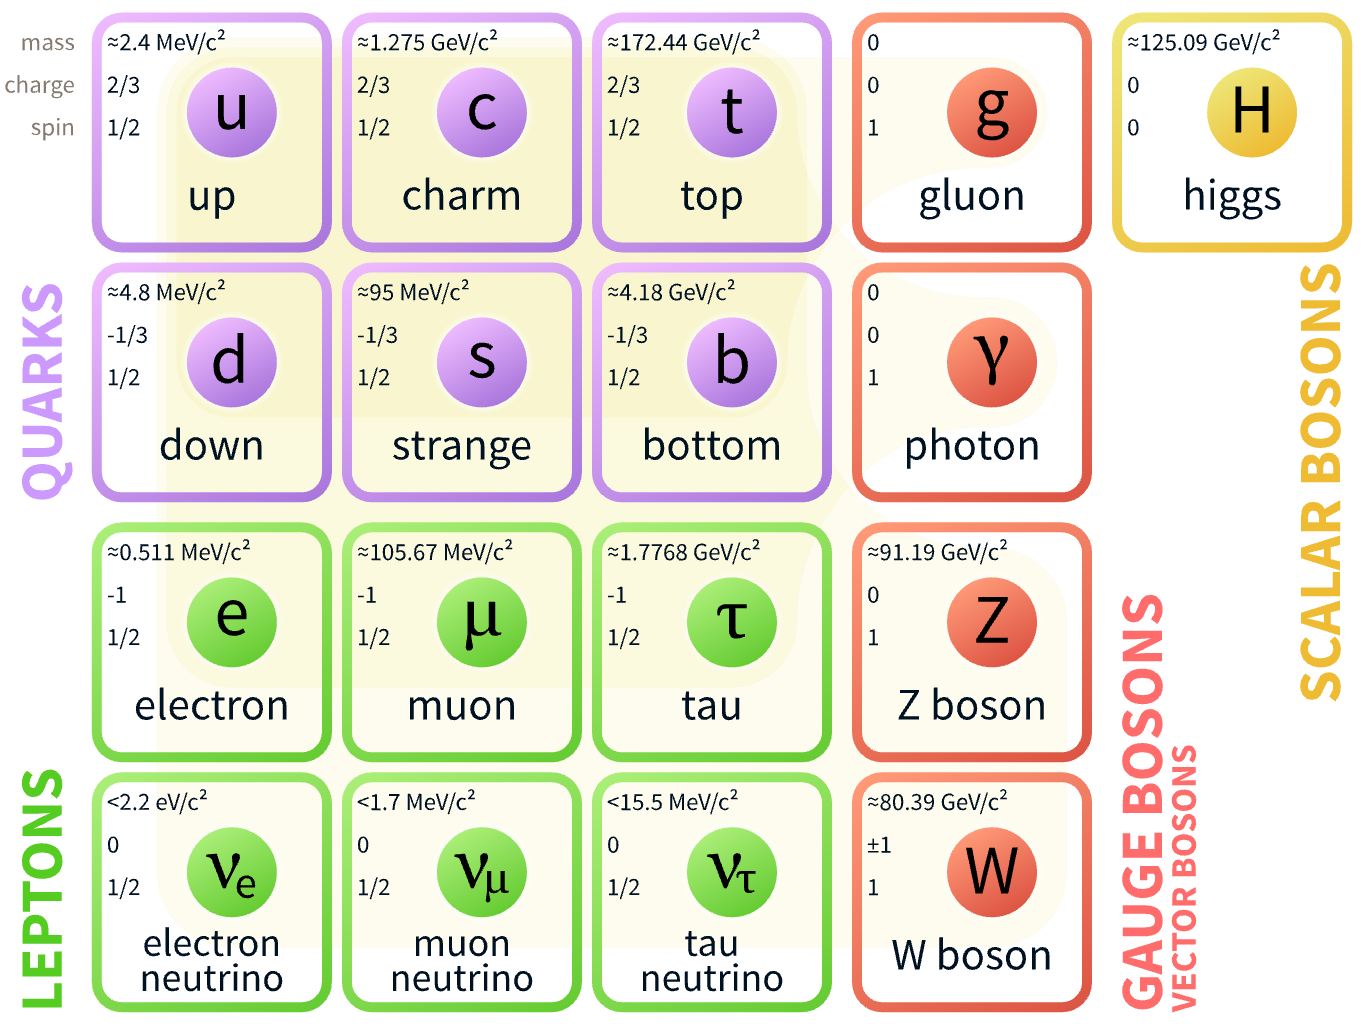
\includegraphics[width=0.6\textwidth]{figures/theory/SM}
  \caption{Fermions and bosons of the Standard Model and their properties~\cite{Pdg}.}
  \label{fig:SM}
\end{figure}

\paragraph{}
However, in SM, due to the gauge invriance under $SU(2)_{L}$, fermions have to be massless in order to have pure left handed states. 
The bosons must also be massless as required by the gauge principle. 
The Higgs mechanism introduces a scalr Higgs field with nonzero vaccum expectation values, which impledes and interacts with the propagation of gague bosons and fermions, hence gives them valid mass terms~\cite{Tully}. 
This broken symmetry of the Standard Model predicts the extra particle degree of freedom as the Higgs boson. The terms inside the Higgs potential are shown in equation~\ref{eqn:higgspotential}.

Include a shape.

\begin{equation}
\label{eqn:higgspotential}
V(\phi_{h}) = \lambda \nu^2 \phi_{h} ^2  + \lambda \nu \phi_{h} ^3  + \frac{1}{4}\lambda \phi_{h} ^4 
\end{equation}

where $\nu$ corresponds to the vaccum expectation value of the field, determined to be around $246$ \GeV.
The first term gives the Higgs mass, $m_h$, as $ \sqrt{2\lambda}\nu$, measured to be $125.09 \pm 0.24$ \GeV. 
The second term provives an $hhh$ vertex, which corresponds to the trilinear coupling of the Higgs boson. 
This means that a two Higgs production (di-Higgs) can happen through a single Higgs even within the Standard Model.

\section{Di-Higgs in the Standard Model}
\paragraph{}
There is much literature about modifications of Higgs self coupling. Using the SM measurements and their precisions, we can constrain the self coupling parameter to an order of magnitude, see \href{https://arxiv.org/abs/1702.07678}{note}.


\section{Di-Higgs in Beyond the Standard Model Physics}


\section{Di-Higgs Decay and search perspectives}

\paragraph{}
Di-Higgs decay is the combination of single Higgs decays. The partile width for Higgs to fermions and bosons (one of them is off-shell) at tree level are shown in equation~\ref{eqn:higgswidth}~\cite{Djouadi}: 

\begin{equation}
\label{eqn:higgswidth}
\begin{array}{cc}
\Tau(h\to f\bar{f} ) = \frac{N_c \sqrt{2} G_{F} m_{f}^2 m_h}{8 \pi} \\
\Tau(h\to VV^{*} ) = \frac{1}{\pi^2} \int_{0}^{M_H^2} \frac{dq_1^2 M_V \Gamma_V}{(q_1^2-M_V^2)^2 + M_V^2\Gamma_V^2} \int_0^{(M_H - q_1)^2} \frac{dq_2^2 M_V \Gamma_V}{(q_2^2-M_V^2)^2 + M_V^2\Gamma_V^2} \frac{\sqrt{2} \delta_v G_{F} m_h^3}{32\pi} \sqrt{\lambda(q_1^2, q_2^2; m_h^2)} [\lambda(q_1^2, q_2^2; m_h^2) + 12\frac{q_1^2q_2^2}{m_h^2}]
%\Tau(h\to WW ) = \frac{2 \sqrt{2} G_{F} m_{W}^2 m_h}{32 \pi} \frac{\sqrt{1 - x_W}}{x_W^2} (3x_W^2 - 4x_w + 4) \\ %only for on shell
%\Tau(h\to ZZ ) = \frac{\sqrt{2} G_{F} m_{z}^2 m_h}{32 \pi} \frac{\sqrt{1 - x_z}}{x_z^2} (3x_z^2 - 4x_z + 4)
\end{array}
\end{equation}
where $N_c$ is the number os colors, $m_f$ is the fermion mass, $G_{F}$ is the Fermi constant. Hence, given the measured Higgs mass, tthe larges brancing ratio is to the \bbbar. Although there is no direct coupling between $h$ and \gg~ at tree level, this decay can happen through W or top loops.

%\paragraph{}CMS latest search result on di-Higgs is also included \href{https://arxiv.org/pdf/1708.08249.pdf}{here}.%Theory
%!TEX root = ../dissertation.tex
\begin{savequote}[75mm]
Pain teaches lessons no scholar can.
% A man who procrastinates in his choosing will inevitably have his choice made for him by circumstance.
% \qauthor{Hunter S. Thompson}
\end{savequote}

\chapter{LHC and ATLAS}
\paragraph{}
The Large Hadron Collider (LHC) is a proton-proton ($pp$) collider at the European Organization for Nuclear Research (CERN) laboratory in Geneva, Switzerland~\cite{LHCPaper}.  ATLAS (A Toroidal LHC ApparatuS), CMS (the Compact Muon Solenoid), ALICE (A Large Ion Collider Experiment), and LHC$b$ (Large Hadron Collider beauty experiment) ~\cite{ATLASPaper, CMSPaper, LHCbPaper, ALICEPaper} are the four main experiments. They are located at the Interaction points(IPs) of the accelerator. Figure~\ref{fig:LHC} shows a schematic of the LHC ring and its experiments. 

\begin{figure}[htbp!]
  \centering
  \captionsetup{justification=centering}
  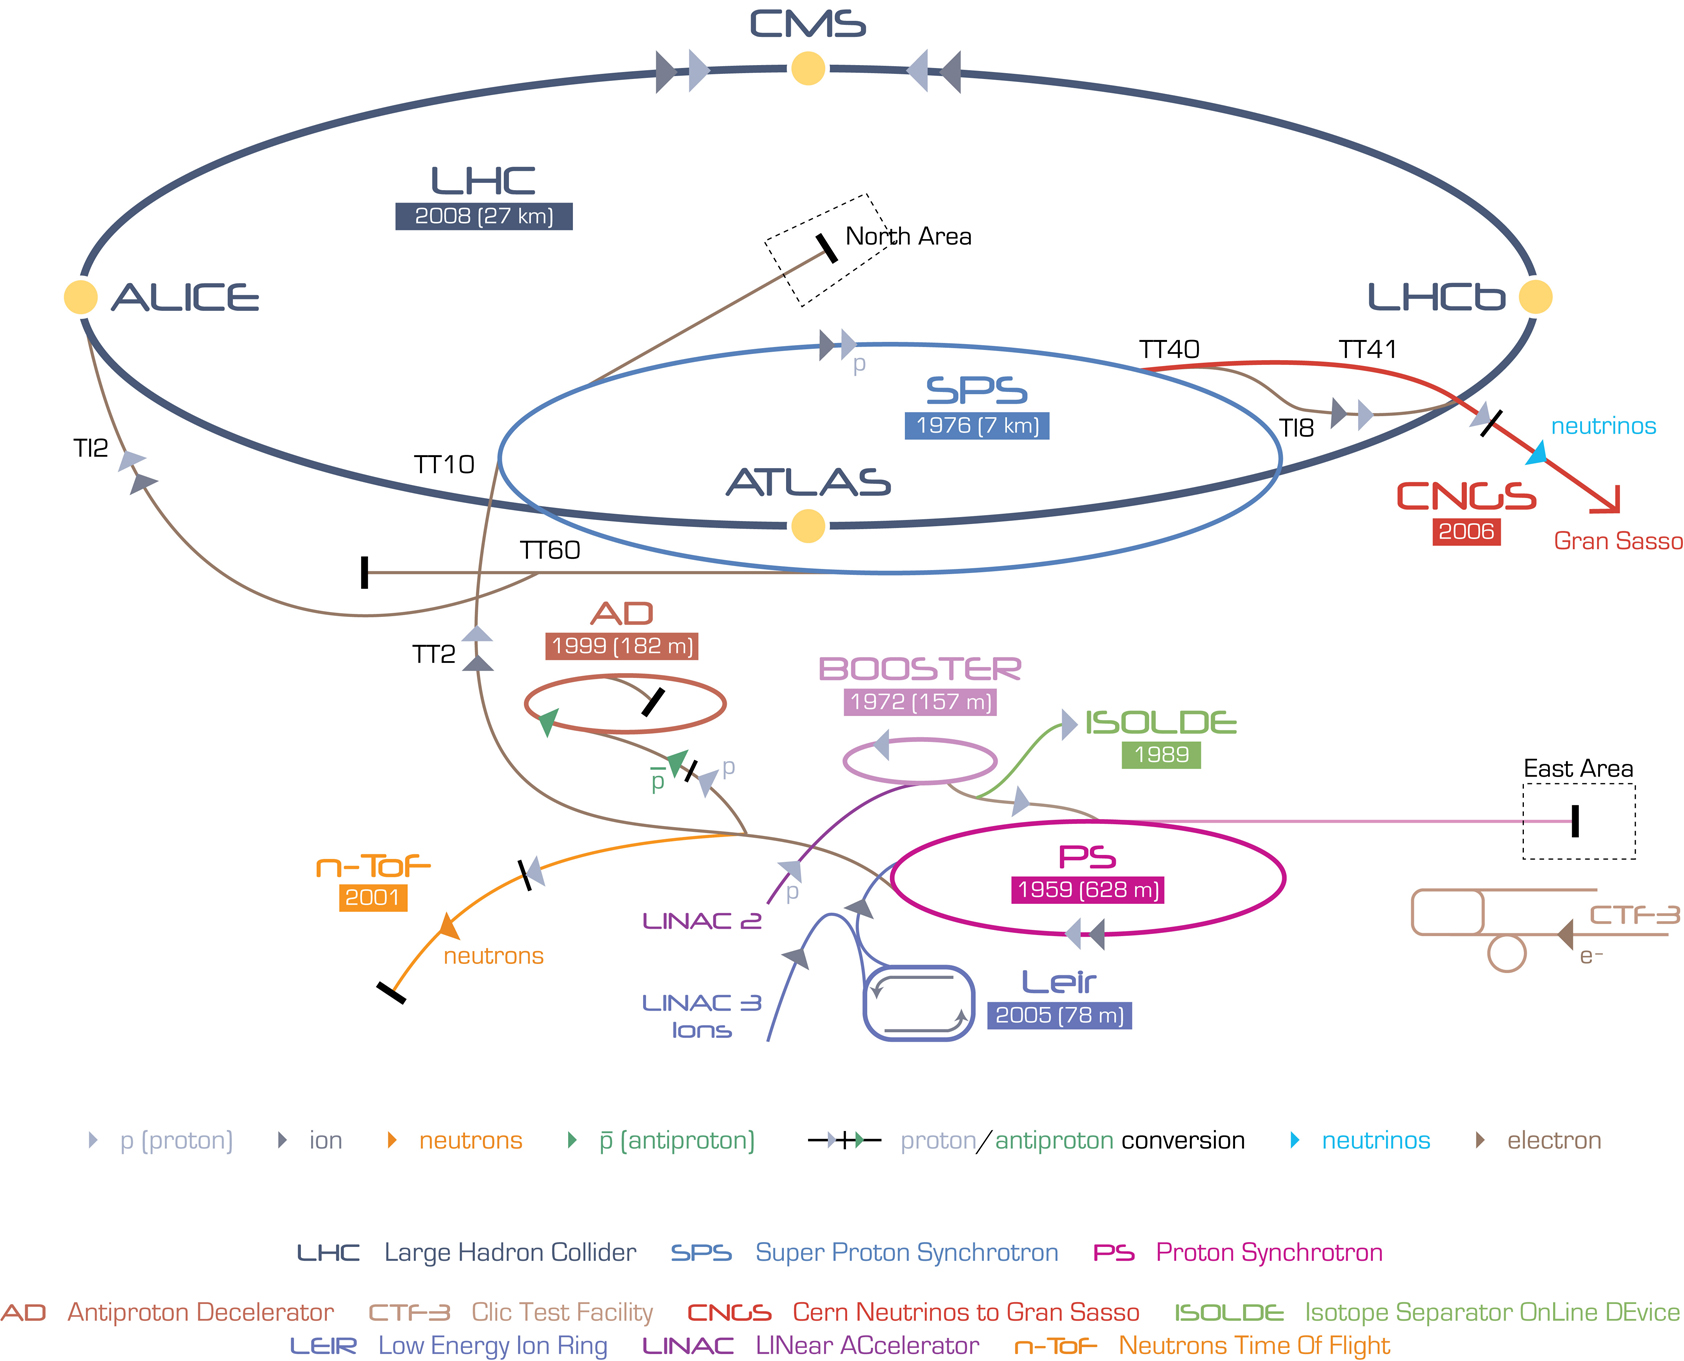
\includegraphics[width=0.6\textwidth]{figures/detector/Cern-Accelerator-Complex.jpg}
   \caption{A schematic view of the LHC ring~\cite{LHCReview}. LINAC2, Booster, PS, SPS, and LHC accelerate the protons in order. Four main experiments are located at interaction points along the ring. ATLAS and CMS are general purpose experiments, while ALICE focuses on heavy ion collisions and LHC$b$ is dedicated to $B$ physics.}
  \label{fig:LHC}
\end{figure}

\section{The Large Hadron Collider}
\label{sec:LHC}
\paragraph{}
Protons accelerated around the LHC originate in a red bottle of hydrogen gas. 
The whole acceleration, taking around 25 minutes, is accomplished in multiple steps:
\begin{itemize}
\item Electrons are stripped from the hydrogens to create protons;
\item A linear particle accelerator, Linac 2, accelerates the protons to $50$ \MeV; 
\item The Proton Synchrotron Booster (PSB) accelerates the protons to $1.4$ \GeV;
\item The Proton Synchrotron (PS) accelerates the protons to $25$ \GeV; 
\item The Super Proton Synchrotron (SPS) accelerates the protons to $450$ \GeV;
\item The $16.7$ kilometers LHC accelerates the protons to the final \TeV~ energies. 
%The LHC uses 1232 Niobium Titanium magnetic dipole for steering the protons. The magnets are cooled by superfluid helium to $1.9$ Kelvin, and can generate $8.33$ Tesla magnetic field.
\end{itemize}

\paragraph{}
The instantaneous luminosity, $L$ ($m^{-2}s^{-1}$), at the LHC is defined in Eq\ref{Ch2:eq-lumi} ~\cite{LHCReview}:
%
\begin{equation}
\label{Ch2:eq-lumi}
L = \frac{n_b N_b^2 f_{\rm rev} \gamma_r}{4\pi \epsilon_n \beta^*} F
\end{equation}
%
In the above Eq\ref{Ch2:eq-lumi}:
\begin{itemize}
	\item $n_b$ is the number of bunches per beam; %$n_b$ cannot be too large due to potential beam loss damages on the accelerator and detector; %Nominally, $2808$ proton bunches.
	\item $N_b$ is the number of protons per bunch;  
	\item $f_{\rm rev}$ is the proton revolution frequency;
	\item $\gamma_r$ is the relativistic Lorentz factor for the protons;
	\item $\epsilon_n$ is the normalized transverse beam emittance, or the average beam spread length;
	\item $\beta^*$ is the transverse beam size; $\sigma_{\rm beam} = \sqrt{\epsilon \cdot \beta}$; %affected by focusing magnets;
	\item $F$ is a reduction factor for the angle beams are colliding. %; smaller crossing angles could cause larger spread in the longitudinal direction.
\end{itemize}

\paragraph{} 
In $pp$ collisions, the rate of a certain physics process is $R_{\rm phy} = L\sigma$, where $\sigma$ ($m^2$) the cross section.
The instantaneous luminosity can also be written as the ratio of the rate of inelastic collisions to the inelastic cross section $\sigma_{\rm inel}$ ~\cite{lumi-paper}:
\begin{equation}
\label{Ch2:eq-lumi2}
L = \frac{R_{\rm inel}}{\sigma_{\rm inel}} = \frac{\mu n_b f_{\rm rev}}{\sigma_{\rm inel}}
\end{equation}
where, $\mu$ is the number of interactions per bunch crossing. 
At each bunch crossing, the collisions without the highest center of mass energy are called ``pileup" interactions.

\begin{table}[]
\centering
\caption[LHC nominal and operational parameters]{LHC nominal~\cite{LHCPaper} and operational parameters in 2015~\cite{LHC_2015} and 2016~\cite{LHC_2016}.}
\begin{tabular*}{\textwidth}{@{\extracolsep{\fill}}llll}
\hline
Parameter [unit]   & Nominal design value & 2015 Operating value  & 2016 Operating value\\
\hline\hline
Beam Energy [TeV]  & $7$  & $6.5$  & $6.5$  \\
Peak L [$10^{34} \text{cm}^{−2}~\text{s}^{-1}$]   & $1$ &   $0.5$  & $1.25$           \\
Bunch spacing [ns]             &      $25$  &  $25$ &      $25$ \\
$f_{\rm rev}$ [kHz]    &     $11245$  & $11245$  & $11245$ \\
$n_b$  [$10^{11}$ p/bunch]   & $1.15$ &  $1.15$ & $1.12$\\
$N_b$  [bunch]         & $2808$   &      $1825$ &      $2220$\\
$\epsilon_n$  [mm mrad]        & $3.5$ &  $3.5$  & $2$\\
$\beta^*$   [cm]         & $55$  &   $40$  & $40$\\
$F$        &      $0.84$  & $0.84$  &  $0.59$ \\
$\langle \mu \rangle$ & $19$ & $13$ & $41$ \\ \hline
\hline            
\end{tabular*}
\label{Ch2:tab-lhc}
\end{table}

\paragraph{}
The main parameters of the LHC beam and performance are shown in Table~\ref{Ch2:tab-lhc}. 
The target peak instantaneous luminosity for both the ATLAS and CMS experiments is $L=10^{34}~\text{cm}^{-2}\text{s}^{-1}$~\cite{LHCPaper}, which has already been exceeded in 2016. 
This is partly due to the improved $\beta^*$ and $F$.
The number of ``pileup" interactions also increases, shown in Figure~\ref{fig:Mu_2015_2016}. 

\begin{figure}[htbp!]
  \centering
  \captionsetup{justification=centering}
  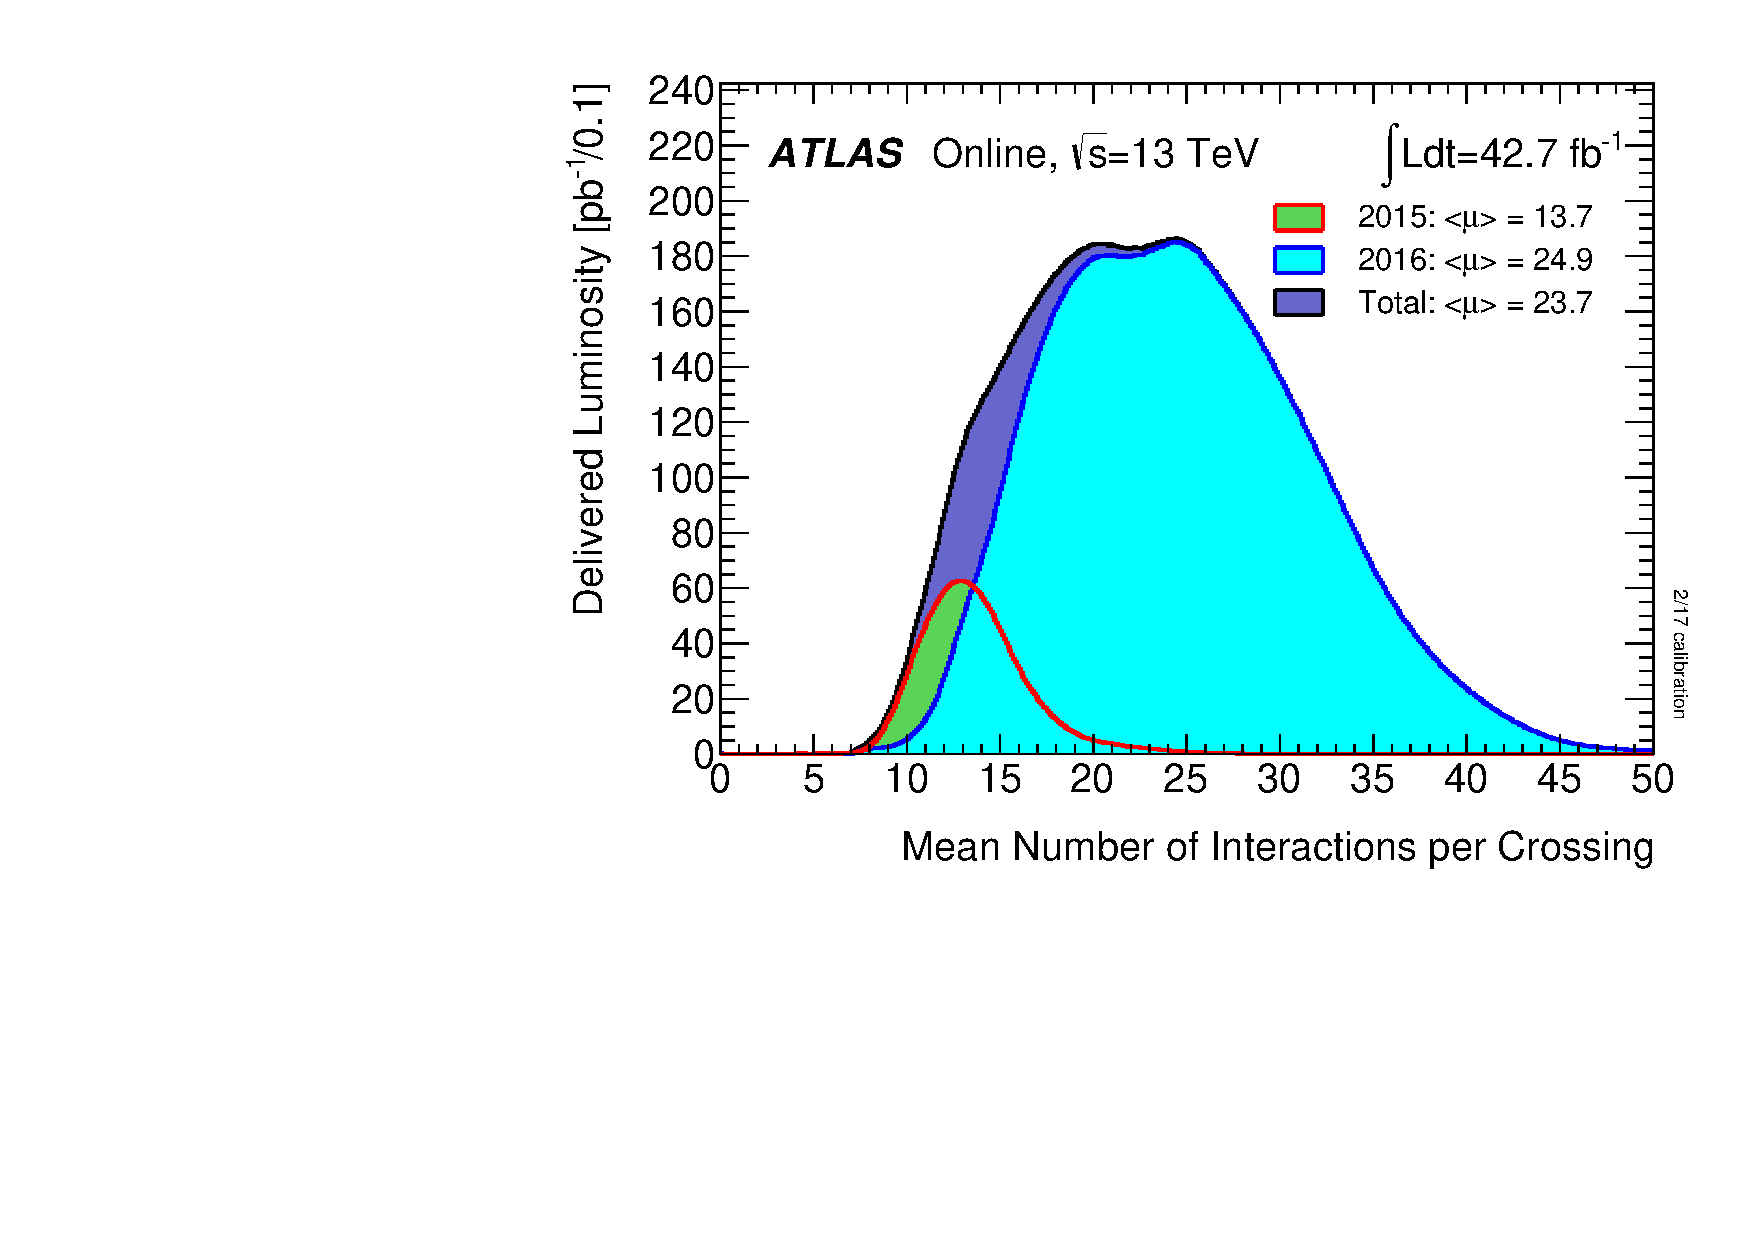
\includegraphics[width=0.5\textwidth,angle=-90]{figures/detector/Mu_2015_2016}
   \caption{The luminosity-weighted distribution of the mean number of interactions per crossing for the 2015 and 2016 $pp$ collision data at $13$ \TeV center-of-mass energy.~\cite{Lumi_Run2}}
  \label{fig:Mu_2015_2016}
\end{figure}
%At the nominal LHC conditions, the beam energy is about 360 MegaJoules, and the LHC in total consumes 115 MegaWatt of power.


\section{A Toroidal LHC ApparatuS}
\label{sec:ATLAS}

\paragraph{}
The ATLAS experiment~\cite{PERF-2007-01} at the LHC is a general-purpose particle detector with a near $4\pi$ coverage in solid angle and a forward-backward symmetric cylindrical geometry. 
The ATLAS detector (Figure~\ref{fig:ATLAS}) consists of an inner tracking detector (ID) surrounded by a $2.3$ m diameter thin superconducting solenoid providing a 2T axial magnetic field, electromagnetic (EM) and hadronic calorimeters, and a muon spectrometer (MS). Three extra air-core toroid magnets generate the magnetic field in the MS. 
%with $1.5$ to $5.5 ~\textrm{T} \cdot\textrm{m}$ of bending power at $0<|\eta|<1.4$ and approximately $1$ to $7.5 ~\textrm{T} \cdot\textrm{m}$ in the endcap region of $1.6 < |\eta| < 2.7$.

\begin{figure}[htbp!]
  \centering
  \captionsetup{justification=centering}
  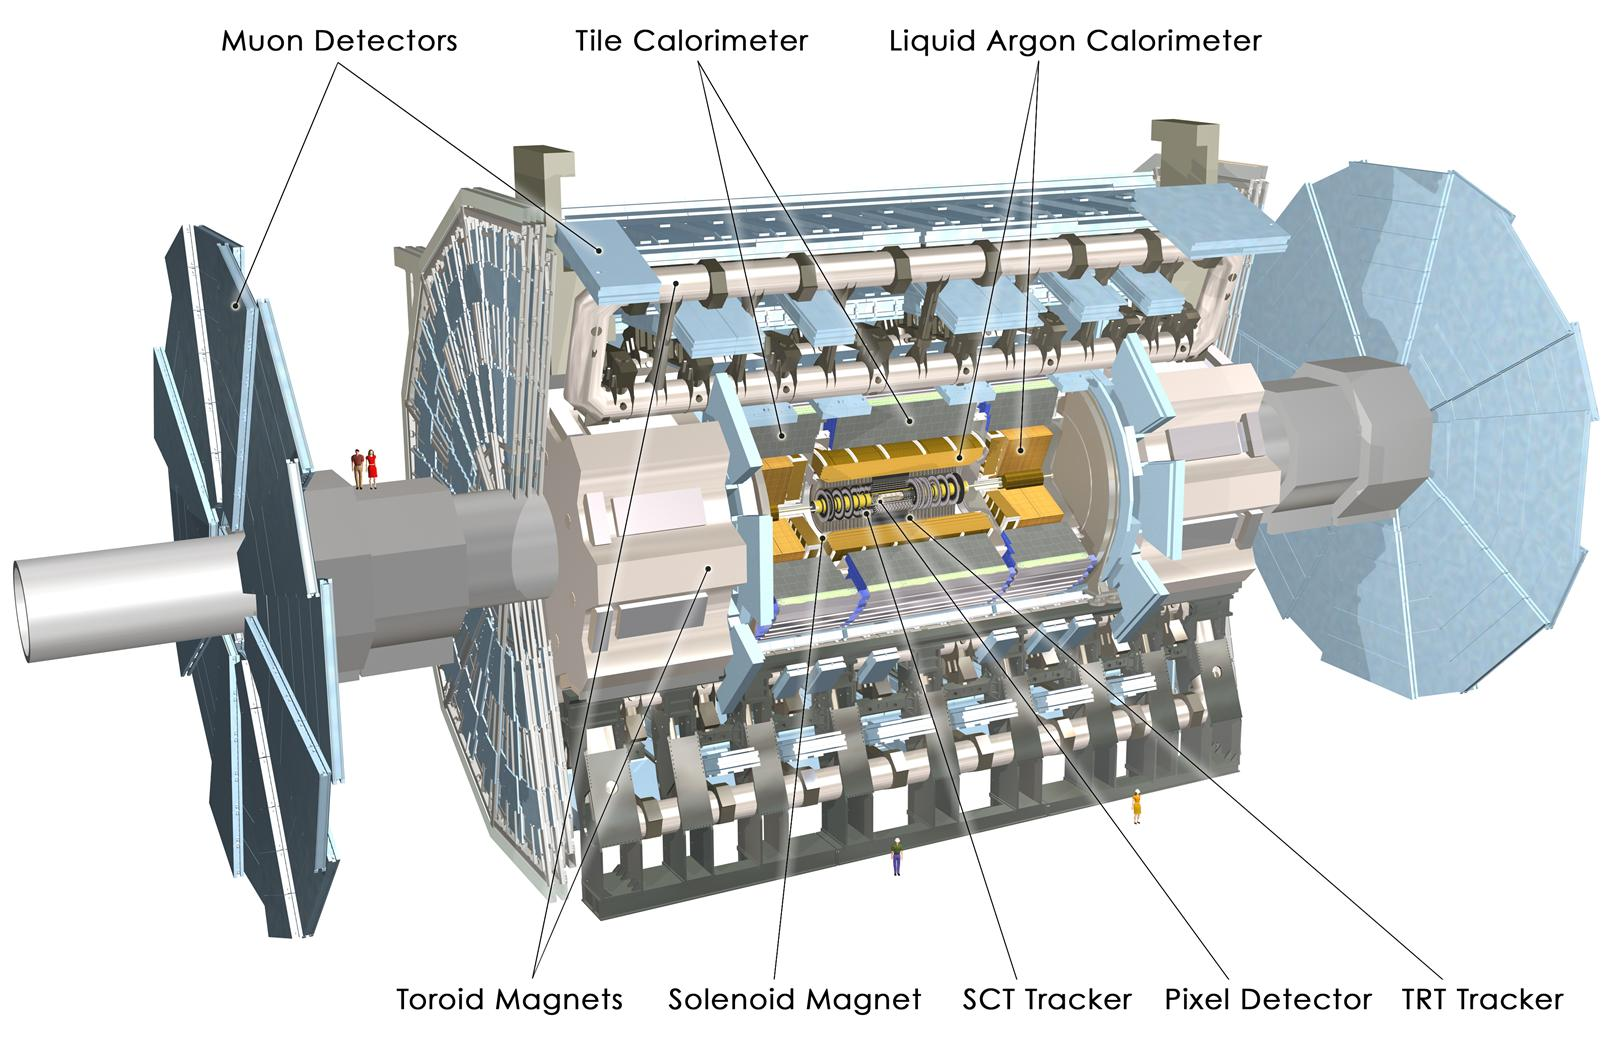
\includegraphics[width=0.7\textwidth]{figures/detector/ATLAS.jpg}
   \caption{A detailed computer-generated image of the ATLAS detector and it's systems.}
  \label{fig:ATLAS}
\end{figure}

%%%%%%%%%%%%%%
\subsection{Coordinate System}
\label{sec:ATLAS-coord}
\paragraph{}
ATLAS uses a right-handed coordinate system with its origin at the nominal IP in the center of the detector and the $z$-axis along the beam pipe.
The positive $x$-axis points from the IP to the center of the LHC ring, the positive $y$-axis points towards the sky, and the $z$-axis points straight(like bridges) towards the Geneva airport(A side), back from the Charlie's pub in France(C side).
Cylindrical coordinates $(r,\phi)$ are used in the transverse plane, $\phi$ being the azimuthal angle around the $z$-axis.
The pseudorapidity is defined in terms of the polar angle $\theta$ as $\eta = -\ln \tan(\theta/2)$. $\eta$ the massless approximation of rapidity $y = \frac{1}{2} \ln \frac{E + p_{z}}{E - p_{z}}$.
$\theta$ is the angle parameterizing special relativity's boosts along the $z$-axis. 
%Most hadron productions are roughly constant in $\eta$, and for two massless particles traveling in different directions, their difference in $\Delta \eta$ is invariant. 
The angular distance is measured in units of $\Delta R = \sqrt{(\Delta\eta)^{2} + (\Delta\phi)^{2}}$.

\paragraph{}
The region with $|\eta| < 1.5$ is called ``central". It consists of the ``barrel" elements, surrounding the beam line cylindrically. For $|\eta| > 1.5$, the region is called ``endcap", and the detector elements are arranged as disks perpendicular to the beam line. At high $|\eta| > 2.5$, the region is referred to as ``forward".

%%%%%%%%%%%%%%
\subsection{Inner Detector}
\paragraph{}
The ID covers the pseudorapidity range $|\eta| < 2.5$.
It consists of three parts: silicon pixel (PIXEL), silicon microstrip (SCT), and straw-tube transition-radiation tracking (TRT) detectors. 
An additional pixel detector layer (IBL) ~\cite{Capeans:1291633}, positioned at a mean radius of $3.3$ cm, is used in the Run-2 data-taking and improves the identification of $b$-jets~\cite{ATL-PHYS-PUB-2015-022}. 
A $10$\GeV~ charged particle in the barrel region expect $1$ IBL hits, $3$ PIXEL hits, $8$ SCT hits and $36$ TRT hits.
Figure~\ref{fig:Det_ID_rz} ~\cite{Aaboud:2017pjd} shows the $R$-$z$ distribution of the material for a quadrant of the barrel region PIXEL and SCT. 
Figure~\ref{fig:Det_ID_xy} shows the distribution of hadronic-interaction vertex candidates in $|\eta|<2.4$ and $|z|<400$ mm for $13$\TeV~ data.
The ID is important for track reconstruction and heavy flavor $b$-tagging. 

%\paragraph{}
%The ID is designed to provide charged particle momentum measurement with $\sigma_{p_{T}}/p_{T} \sim 0.05\% p_{T} \oplus 1\%$ and vertex reconstruction.
%Because of this, each detector proves measurement accuracies of the order $10 \mu\rm m$ in $R$-$\phi$ and $100 \mu\rm m$ in $z$.
%The intensity of a particle beam decreases exponentially in radiation length. $I(x) = I_0 e^{-x/X_0}$, where $I$ is the intensity, $x$ is the distance traveled, and $X_0$ is the radiation length.

\begin{figure}[htbp!]
\centering
\captionsetup{justification=centering}
    \begin{subfigure}[b]{0.6\textwidth}
        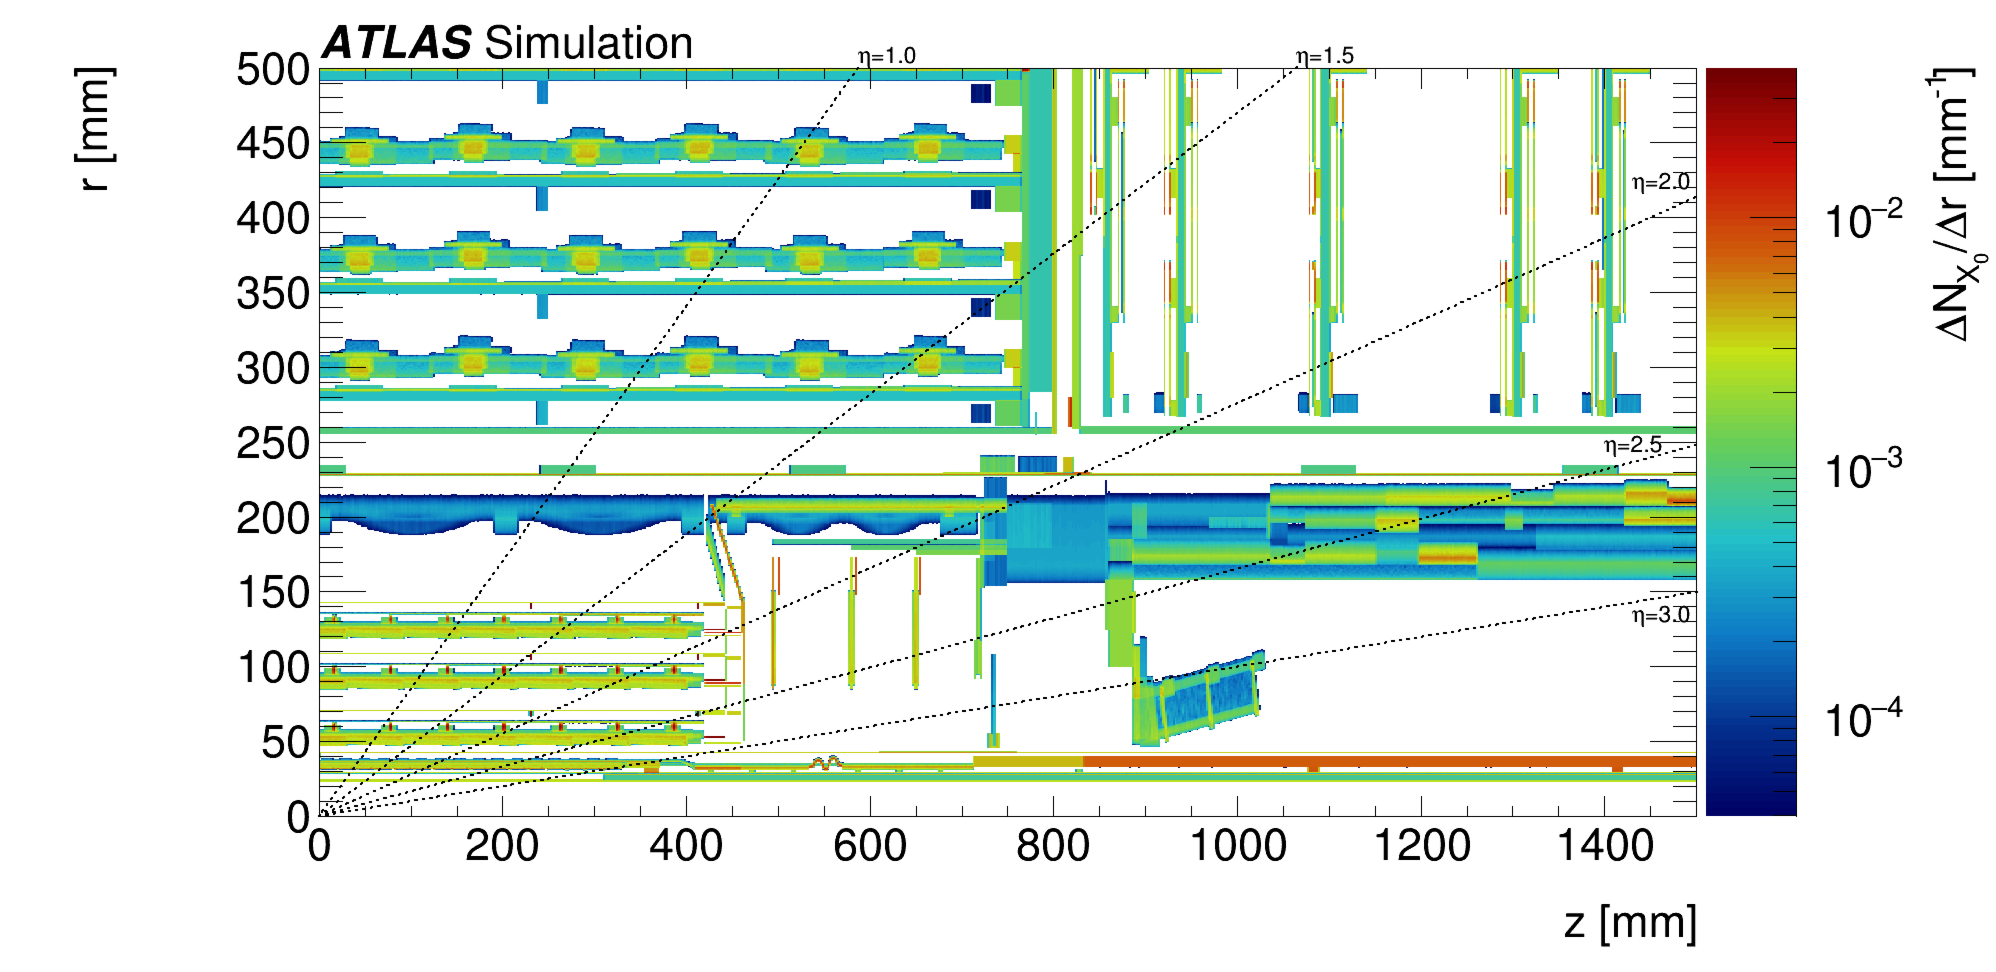
\includegraphics[width=\textwidth]{figures/detector/ID_rzmap}
        \caption{The $R$-$z$ distribution of material's differential number of radiation lengths, $\frac{\Delta N_{X_0}}{\Delta r}$}
        \label{fig:Det_ID_rz}
    \end{subfigure}
    \quad
    \begin{subfigure}[b]{0.3\textwidth}
        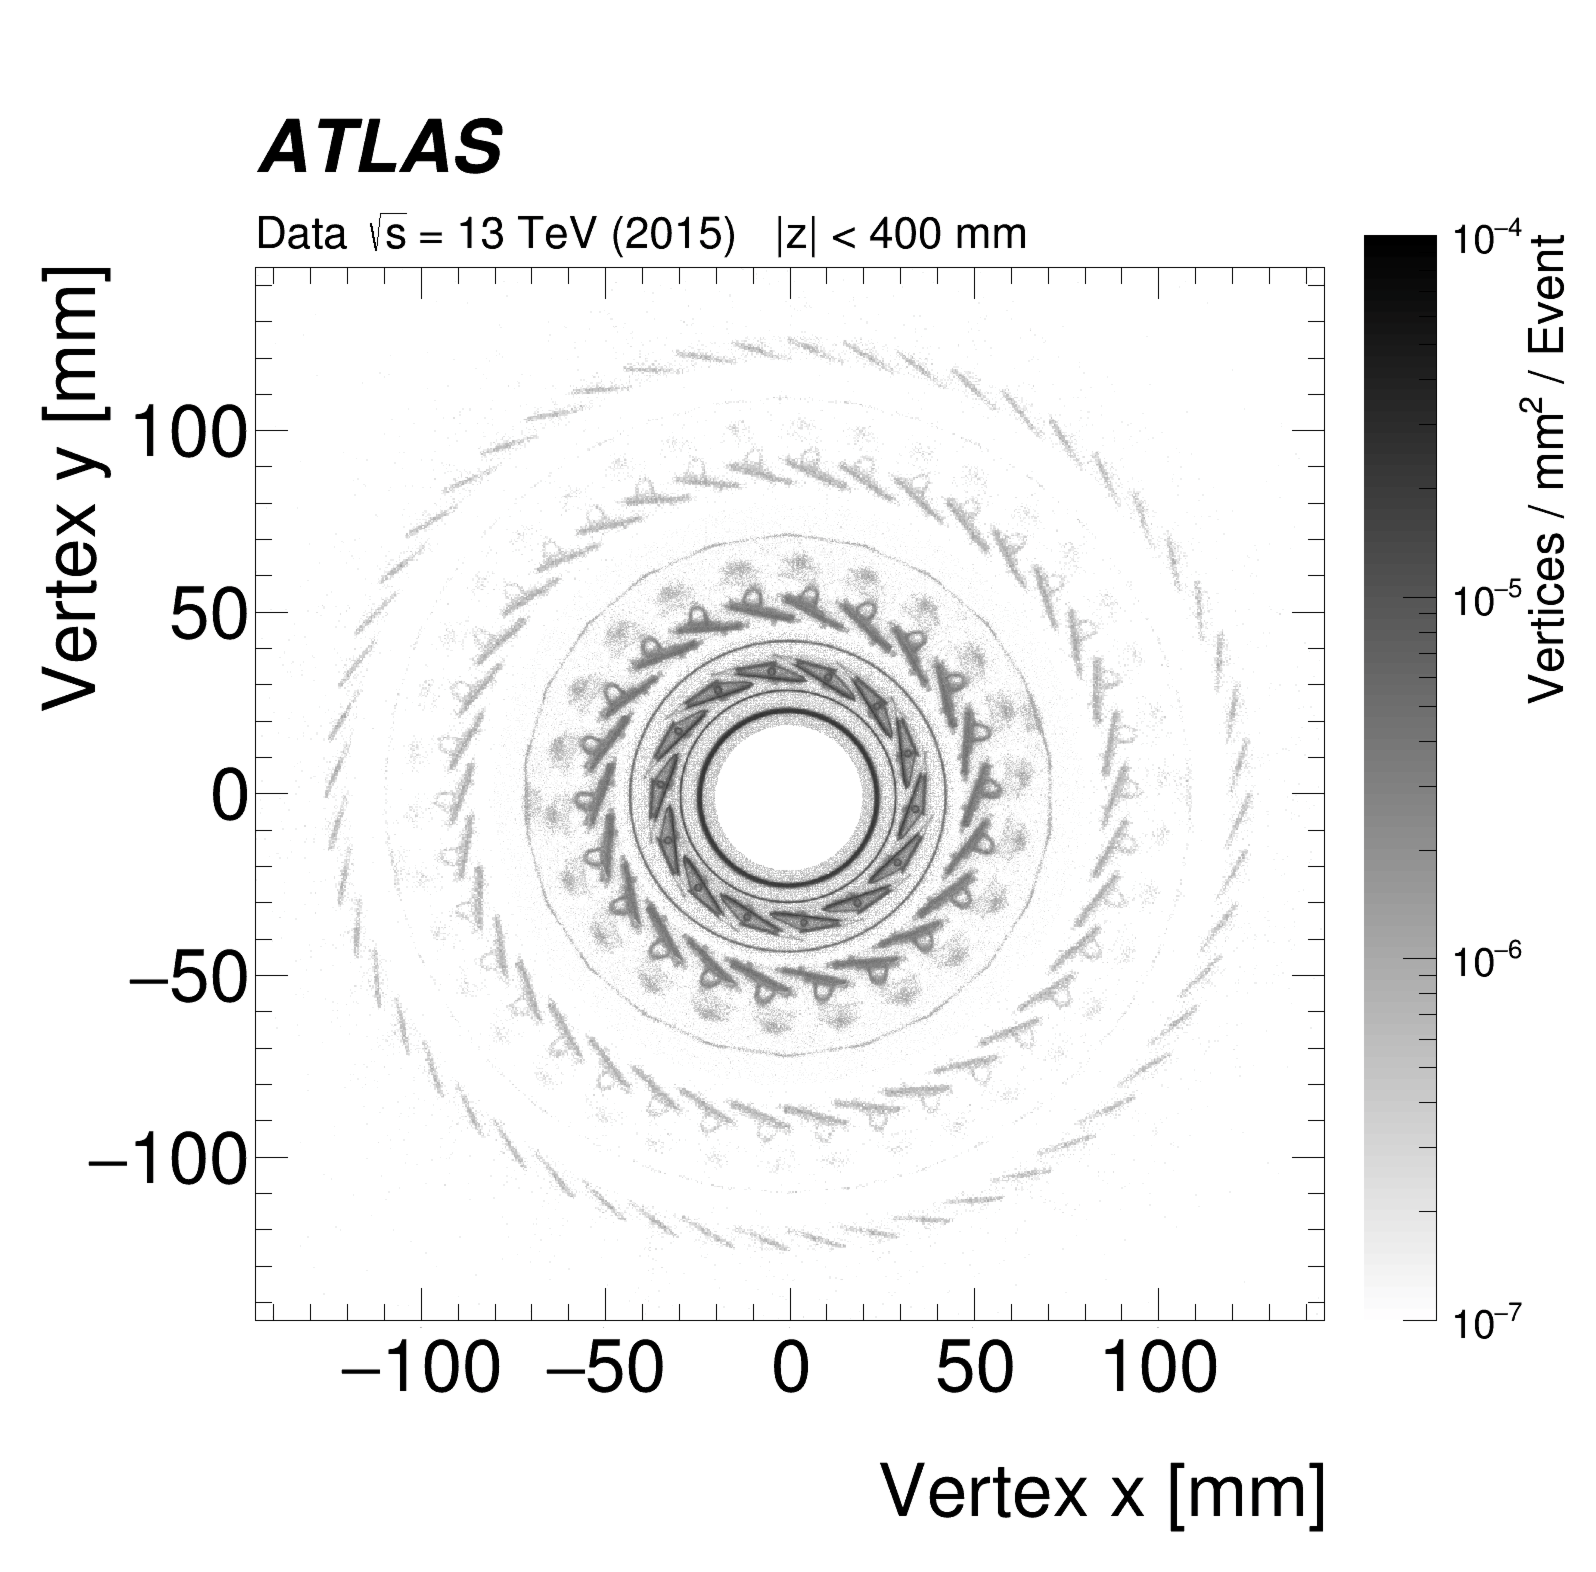
\includegraphics[width=\textwidth]{figures/detector/ID_data_map_XY}
        \caption{Distribution of hadronic-interaction vertex candidates}
        \label{fig:Det_ID_xy}
    \end{subfigure}
\caption{Gemoetry of IBL, PIXEL and SCT detectors in Run2.}
\label{fig:Det_ID}
\end{figure}

%Material of ATLAS Inner Detector for Run 2 of the LHC. \href{https://cds.cern.ch/record/2260595/files/PERF-2015-07-002.pdf}{note}.
%%%%%%%%%%%%%%
\subsection{Calorimeter}
\paragraph{}
The Lead/liquid-argon (LAr) finely segmented sampling calorimeters provide EM energy measurements. 
A steel/scintillator-tile hadronic calorimeter covers the central pseudorapidity range ($|\eta| < 1.7$).
The endcap and forward regions are instrumented with copper/tungsten and LAr calorimeters for both the EM and hadronic energy measurements up to $|\eta| = 4.9$. The calorimeters also provide basic EM/Hadronic trigger information, with fast analogue summing in coarse granularity.
The calorimeters are important for measuring the energy of the Higgs boson decay productions.

%\paragraph{}
%EM calorimeter (ECal) is designed to have $>22$ radiation lengths in the barrel and $> 24$ in the endcap. 
%It provides EM measurement with $\sigma_E/E = 10\%/\sqrt{E} \oplus 0.7\%$. The hadronic calorimeter (HCal) has approximately $9.7$ interaction length in the barrel and $10$ in the endcap. 
%HCal provides hadronic measurement with $\sigma_E/E = 50\%/\sqrt{E} \oplus 3\%$ in the Barrel and Endcap regions, and $\sigma_E/E = 100\%/\sqrt{E} \oplus 10\%$  in the forward region.

%%more plots: https://twiki.cern.ch/twiki/bin/view/AtlasPublic/LArCaloPublicResults2015

%%%%%%%%%%%%%%
\subsection{MuonSpectrometer}

\begin{figure}[htbp!]
\centering
\captionsetup{justification=centering}
    \begin{subfigure}[b]{0.5\textwidth}
        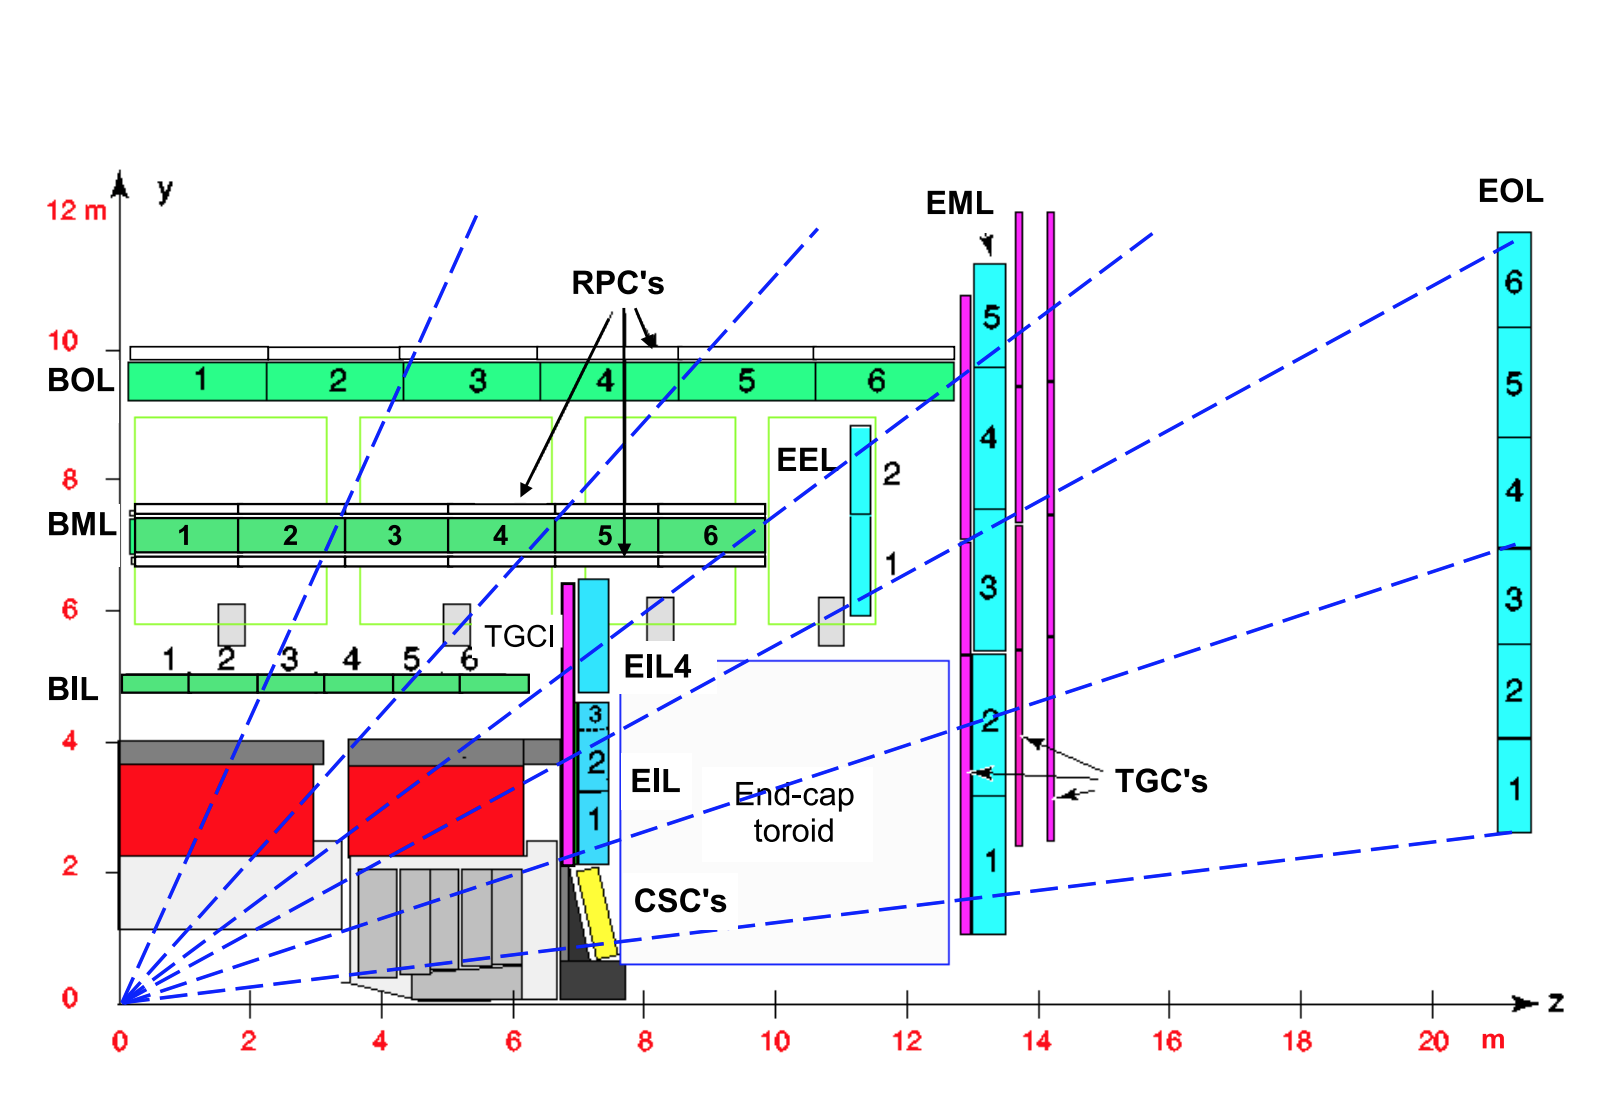
\includegraphics[width=\textwidth]{figures/detector/MS_rz}
        \caption{Cross-section of the muon system in $R$-$z$ plane. Numbers indicate different $\eta$ stations. For MDT letters, B means barrel, and E means endcap. I stands for inner, M for middle, O for outer, and E for extra.}
        \label{fig:MS_rz}
    \end{subfigure}
    \quad
    \begin{subfigure}[b]{0.3\textwidth}
        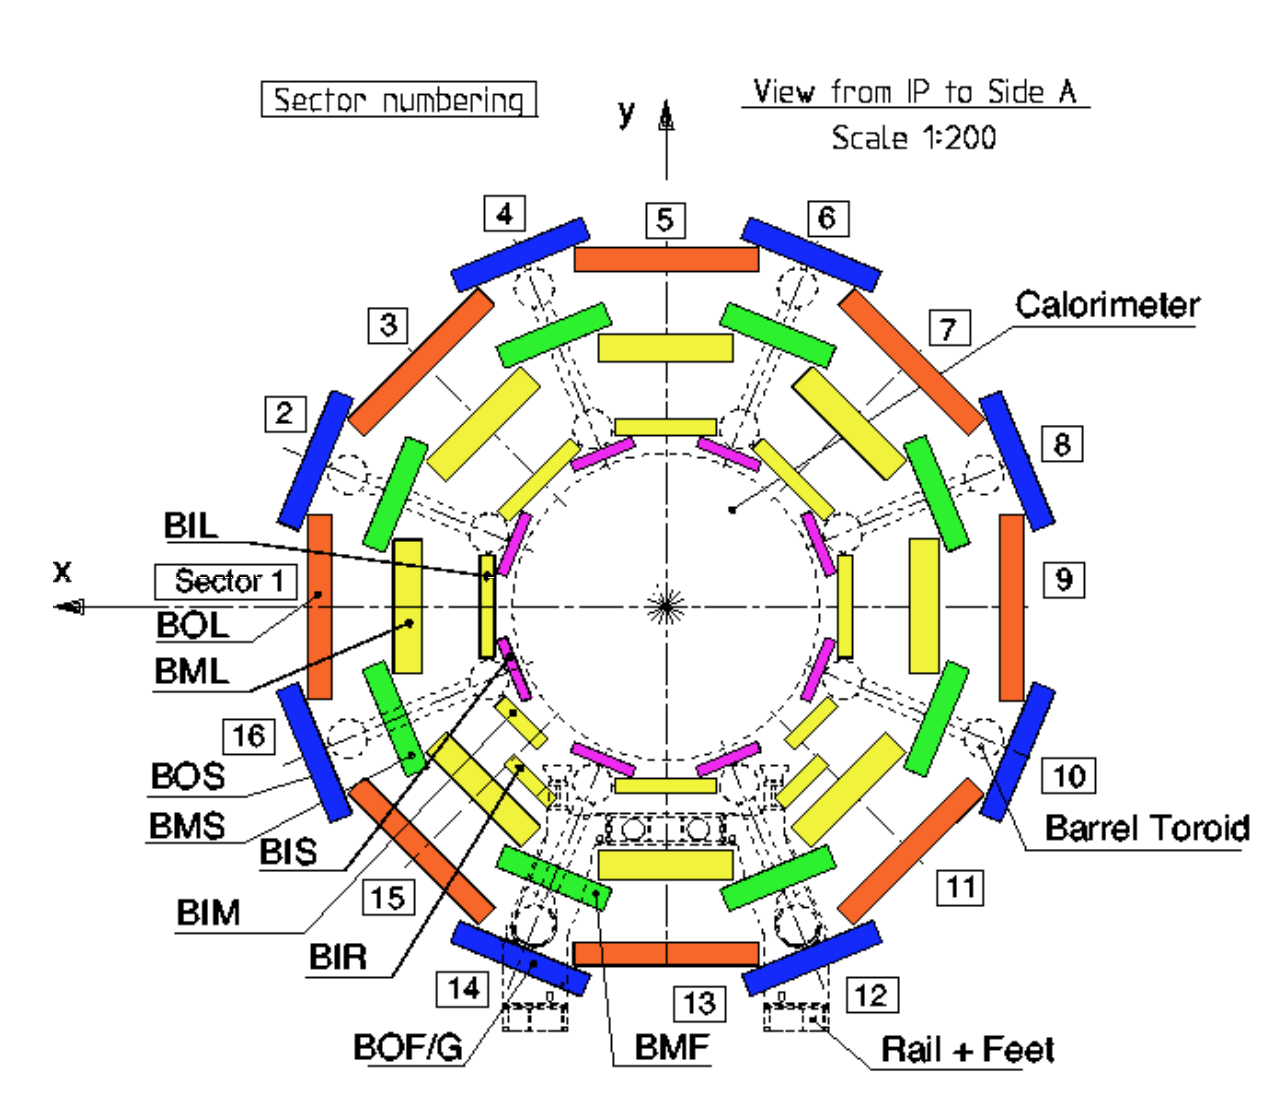
\includegraphics[width=\textwidth]{figures/detector/MS_phi}
        \caption{Cross-section of the barrel muon system in $x$-$y$ plane. Numbers indicate different $\phi$ stations. Last L means large sectors and last S means small sectors.}
        \label{fig:MS_phi}
    \end{subfigure}
\caption{The overall layout of the ATLAS MuonSpectrometer.}
\label{fig:Det_MS}
\end{figure}

\paragraph{}
The muon spectrometer (Figure~\ref{fig:Det_MS}) is the largest component of the ATLAS detector.
It surrounds the calorimeters and includes three large superconducting air-core toroids. 
The field integral of the toroids ranges between 2 and 6 T/m for most of the detector. Because of this bending power, the MS measures Muon momentum stand-alone, with $\sigma_{p_{T}}/p_{T} \sim 10\%$ at $p_{T} = 1$\TeV. 
Muon Drift Tubes (MDT) and Cathode Strip Chambers (CSC) provide precision tracking. 
%Each MDT has $80\,\mu\textrm{m}$ single hit spacial resolution, with an alignment precision of $30\,\mu\textrm{m}$.
Resistive Plate Chambers (RPC) in the barrel and Thin Gap Chambers (TGC) provide triggering, with $1.5$-$5$ ns timing resolution. 

%%%%%%%%%%%%%%
\subsection{Trigger and Data Acquisition}
\paragraph{}
A dedicated trigger system is used to select events~\cite{ATLAS-TRIGGER}.
The first-level trigger (L$1$) is implemented in hardware and uses the calorimeter and muon detectors to seed regions of interest (RoI) and reduce the accepted event rate to $100$ kHZ.
This is followed by a software-based high-level trigger (HLT) that reduces the accepted event rate to $1$ kHZ on average. 
To avoid high rates for certain triggers, the triggers are often prescaled, which means some accepted events get rejected. 
For example, a prescale of two means only every second event passing all trigger conditions gets accepted. 

\paragraph{}
Over 2015 and 2016, both the LHC and the ATLAS performed outstandingly ~\cite{Lumi_Run2}. The total data recording efficiency for ATLAS is around $92\%$, shown in Figure~\ref{fig:Lumi}.

\begin{figure}[htbp!]
\centering
\captionsetup{justification=centering}
	\hspace{-2cm}
    \begin{subfigure}[b]{0.35\textwidth}
        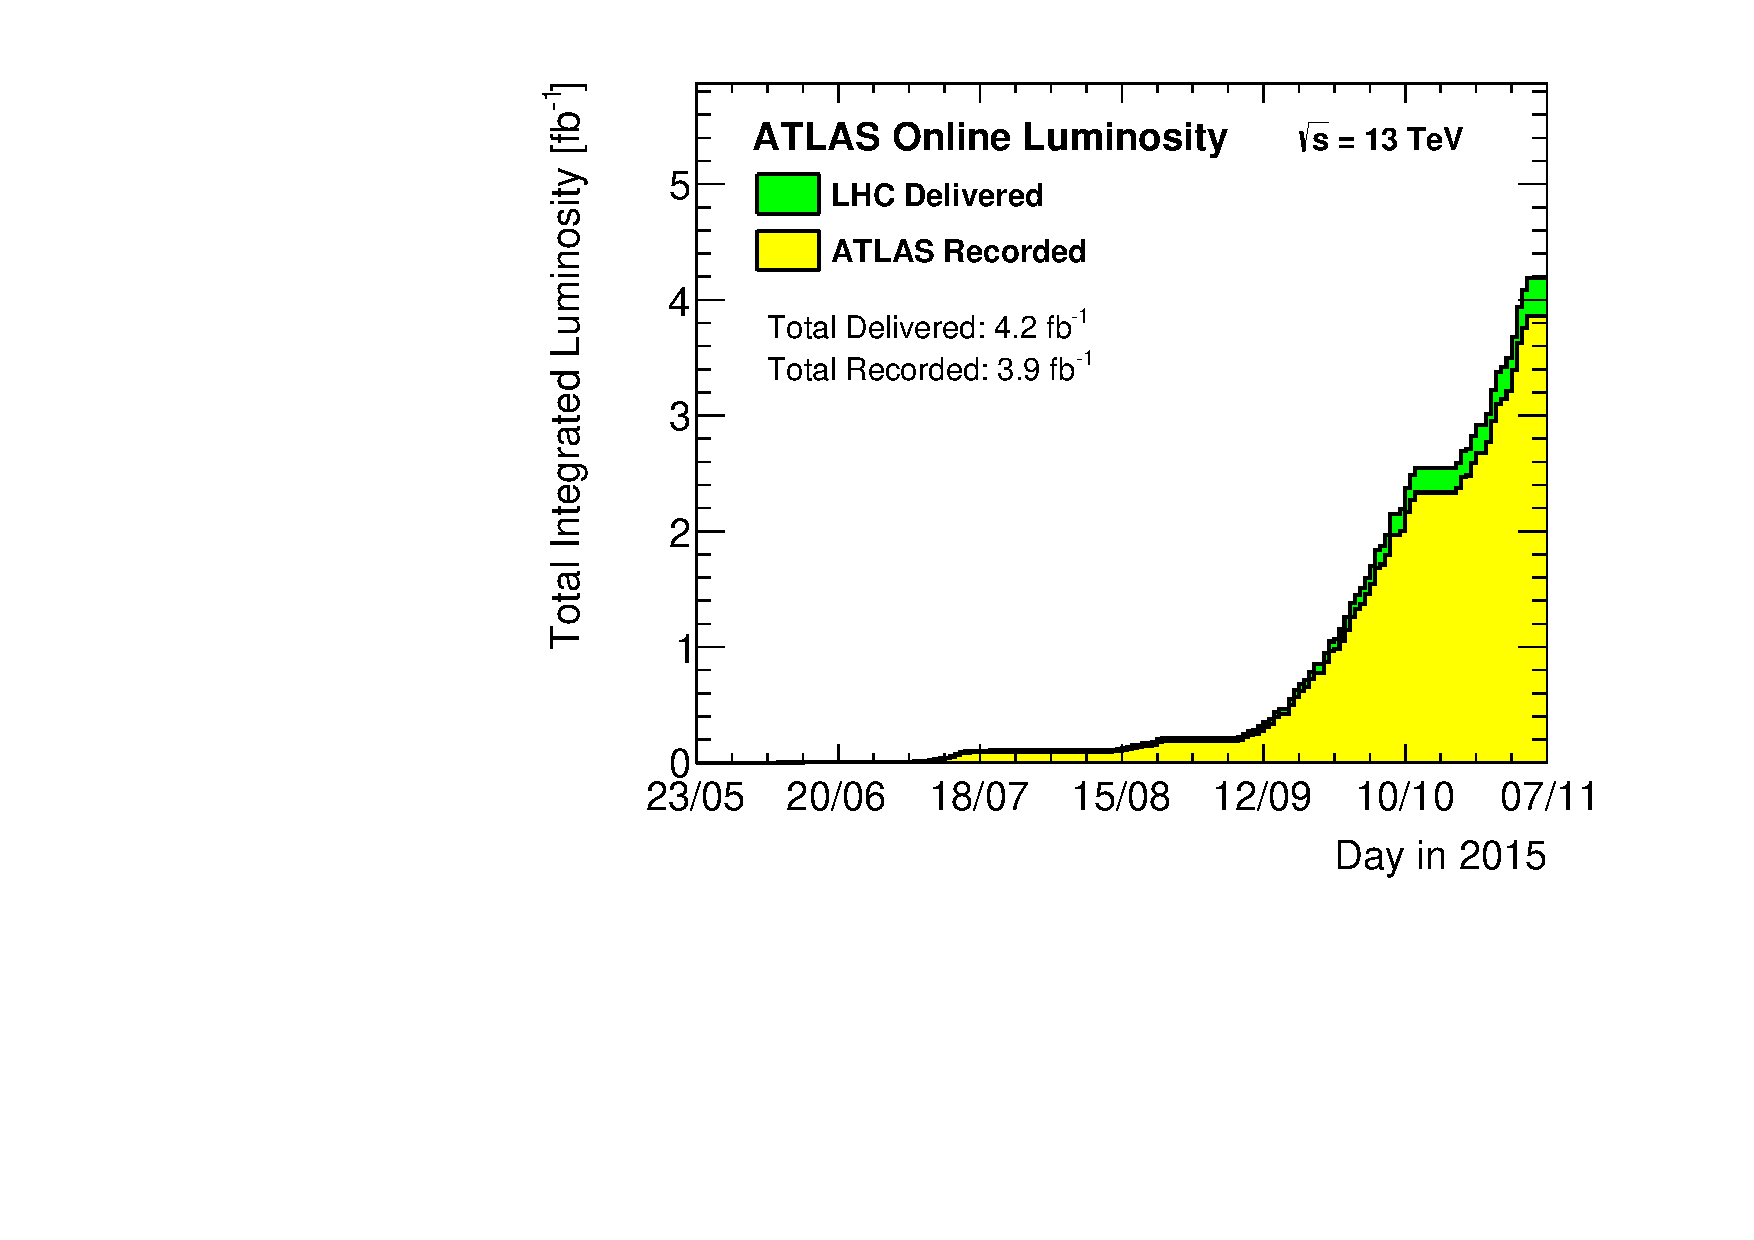
\includegraphics[width=\textwidth,angle=-90]{figures/detector/Lumi_2015}
        \caption{2015}
        \label{fig:Lumi_2015}
    \end{subfigure}
    \quad
    \quad
    \quad
    \quad
    \begin{subfigure}[b]{0.35\textwidth}
        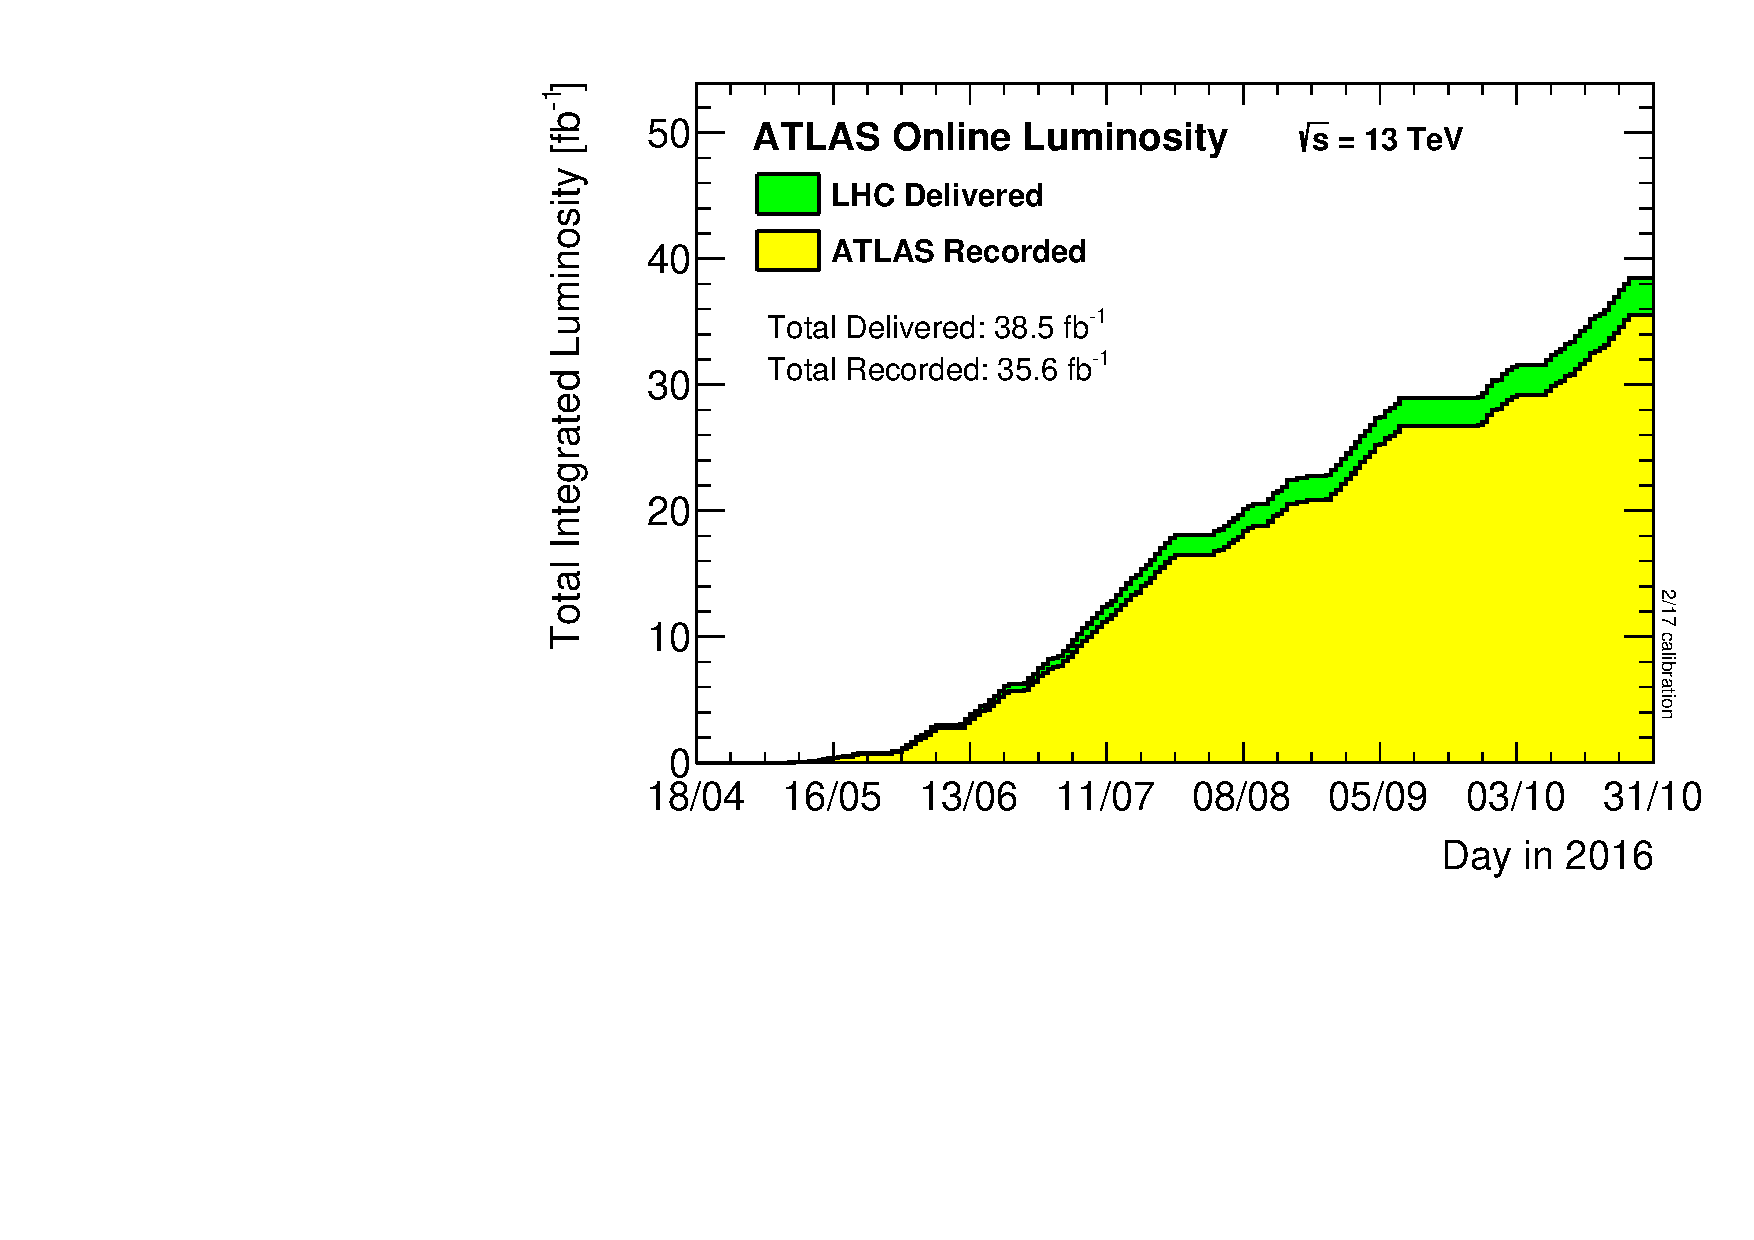
\includegraphics[width=\textwidth,angle=-90]{figures/detector/Lumi_2016}
        \caption{2016}
        \label{fig:Lumi_2016}
    \end{subfigure}
\caption{Cumulative luminosity vs. time delivered to (green) and recorded by ATLAS (yellow) during stable beams for $pp$ collisions at $13$ \TeV centre-of-mass energy.}
\label{fig:Lumi}
\end{figure}

% \paragraph{}
% For further trigger information, see \href{http://atlas.web.cern.ch/Atlas/GROUPS/PHYSICS/PAPERS/TRIG-2016-01/}{2015 note} and \href{https://cds.cern.ch/record/2242069/files/ATL-DAQ-PUB-2017-001.pdf}{2016 updates}.





%LHC, ATLAS
%!TEX root = ../dissertation.tex
\begin{savequote}[75mm]
Ugliness is in a way superior to beauty because it lasts.
\qauthor{Serge Gainsbourg}
\end{savequote}
%%%%%%%%%%%%%%
\chapter{Data and Simulation}%Reco
%!TEX root = ../dissertation.tex
\begin{savequote}[75mm]
Ugliness is in a way superior to beauty because it lasts.
\qauthor{Serge Gainsbourg}
\end{savequote}
%%%%%%%%%%%%%%
\chapter{Data and Simulation}
%\subsection{Dataset}

\paragraph{}
The studies presented in this note are based on the 2015 and 2016 dataset at $\sqrt{s}=13$~TeV recorded by the ATLAS experiment~\cite{detPaper}. Jet triggers were used to select the data (details below). The analysis also ran over the 2015 and the 2016 debug stream, in which no events that pass the full event selection were found. The 2015 dataset corresponds to a total integrated luminosity of 3.2\, fb$^{-1}$, and the 2016 dataset corresponds to a total integrated luminosity of 32.9\, fb$^{-1}$. The total luminosity is 36.1\, fb$^{-1}$.

\paragraph{}
The analysis is based on EXOT8 derivations of the xAOD, the contents of which can be found at \href{https://svnweb.cern.ch/trac/atlasoff/browser/PhysicsAnalysis/DerivationFramework/DerivationFrameworkExotics/trunk/share/EXOT8.py}{DerivationFrameworkExotics/EXOT8}. The 20.7.8.7 derivation cache was used in the analysis, which corresponds to \texttt{DerivationFrameworkExotics-00-03-86} and $p$-tags \texttt{p2950}. The boosted slimming keeps events with at least two large-$R$ jets with \pt~$>$200 GeV. 
%In the derivationt here is another cut requiring there are at least two trackjets with MV2c10 score greater than -10. Because there is no pT cut, this requirement is almost always passed--events doesn't pass this hints the large-R jet has one and only one tracking activities, which is also probably a good idea to keep it out. However, this should be modified in the future.

\paragraph{}
The studies presented currently in the main context of this note are extended to incorporate 2016 data. In this note, the reconstruction of both the 2015 and 2016 datasets are performed using software release 20.7. Simulated data samples from the mc15c campaign are be used, corresponding to $p$-tags \texttt{p2952-p2949}.
% to look up derivation tag info:
% > grep Exotics /cvmfs/atlas.cern.ch/repo/sw/software/x86_64-slc6-gcc48-opt/20.1.8/AtlasDerivation/20.1.8.5/AtlasDerivationRelease/cmt/requirements
% https://twiki.cern.ch/twiki/bin/viewauth/AtlasProtected/DerivationProductionTeam#Info_on_AtlasDerivation_caches_a

\paragraph{}
The 2015 data sets from release 20.7 that are currently used in this analysis are:
\noindent
\\
{\scriptsize
\verb|data15_13TeV.periodD.physics_Main.PhysCont.DAOD_EXOT8.grp15_v01_p2950|\\
\verb|data15_13TeV.periodE.physics_Main.PhysCont.DAOD_EXOT8.grp15_v01_p2950|\\
\verb|data15_13TeV.periodF.physics_Main.PhysCont.DAOD_EXOT8.grp15_v01_p2950|\\
\verb|data15_13TeV.periodG.physics_Main.PhysCont.DAOD_EXOT8.grp15_v01_p2950|\\
\verb|data15_13TeV.periodH.physics_Main.PhysCont.DAOD_EXOT8.grp15_v01_p2950|\\
\verb|data15_13TeV.periodJ.physics_Main.PhysCont.DAOD_EXOT8.grp15_v01_p2950|
}

\paragraph{}
The current 2016 data sets are:
\noindent
\\
{\scriptsize
\verb|data16_13TeV.periodA.physics_Main.PhysCont.DAOD_EXOT8.grp16_v01_p2950|\\
\verb|data16_13TeV.periodB.physics_Main.PhysCont.DAOD_EXOT8.grp16_v01_p2950|\\
\verb|data16_13TeV.periodC.physics_Main.PhysCont.DAOD_EXOT8.grp16_v01_p2950|\\
\verb|data16_13TeV.periodD.physics_Main.PhysCont.DAOD_EXOT8.grp16_v01_p2950|\\
\verb|data16_13TeV.periodE.physics_Main.PhysCont.DAOD_EXOT8.grp16_v01_p2950|\\
\verb|data16_13TeV.periodF.physics_Main.PhysCont.DAOD_EXOT8.grp16_v01_p2950|\\
\verb|data16_13TeV.periodG.physics_Main.PhysCont.DAOD_EXOT8.grp16_v01_p2950|\\
\verb|data16_13TeV.periodI.physics_Main.PhysCont.DAOD_EXOT8.grp16_v01_p2950|\\
\verb|data16_13TeV.periodK.physics_Main.PhysCont.DAOD_EXOT8.grp16_v01_p2950|\\
\verb|data16_13TeV.periodL.physics_Main.PhysCont.DAOD_EXOT8.grp16_v01_p2950|
}


\clearpage
\subsection{Simulated signal and background samples}
\paragraph{}
All MC samples used in this analysis are produced with full simulation, with additional \pileup interactions in each simulated event 
modeled by adding multiple soft $pp$ collisions
generated by \Pythia~8.165~\cite{pythia8} with the MSTW2008 LO PDF and AU2 tune~\cite{MC12AU2}.  After event generation and the addition of \pileup, 
the response of the ATLAS detector to particles
passing through the detector elements is simulated with the GEANT4 toolkit~\cite{Geant4,simulation}
and events are reconstructed using the same software used to reconstruct events in data.
%Simulation events are further corrected to reproduce the amount of pileup produced in the data, using the standard ATLAS pileup reweighting tool~\cite{pileuptwiki}.

\subsubsection{Signal MC production}
%A non-resonant SM signal sample has been generated using aMC@NLO. These \ggtofourb events are generated at NLO, using the exact form factors for the top loop taken from HPAIR~\cite{PhysRevD.58.115012,Plehn199646}. The sample is:
%\begin{Verbatim}[fontsize=\scriptsize]
%mc15_13TeV.342619.aMcAtNloHerwigppEvtGen_UEEE5_CTEQ6L1_CT10ME_hh_4b.merge.DAOD_EXOT8.e4419_s2608_r6869_r6282_p2454.
%\end{Verbatim}

%The gluon-fusion production cross-section used is evaluated at NNLO+NNLL in QCD \cite{LHCHXSWGHH}: $\sigma(pp\rightarrow hh\rightarrow b\bar{b}b\bar{b})~=~12.7\pm1.6$\,fb, where the uncertainty term includes the effects of uncertainties in the renormalization and factorization scale, PDFs, $\alpha_S$, effects of finite $m_t$ in loops and $Br\left(H\rightarrow b\bar{b}\right)$.
%, summed with the NLO predictions for vector-boson-fusion, top-pair-associated and vector-boson-associated production from Ref.~\cite{1401.7340}. The resulting cross-section is $\sigma(pp\rightarrow hh\rightarrow b\bar{b}b\bar{b}) = 3.6\pm0.5$\,fb, where the uncertainty term includes the effects of uncertainties in the renormalization and factorization scale, PDFs, $\alpha_S$ and $Br\left(H\rightarrow b\bar{b}\right)$.

\paragraph{}
Two benchmark resonant signal models are considered: a spin-2 graviton within a Bulk Randall-Sundrum Kaluza-Klein model and a spin-0 heavy neutral Higgs boson within a 2HDM model. 

\paragraph{}
The Bulk RS KK graviton signal samples have been generated for 20 mass points from 300 to 3000\,GeV using the \Madgraph generator\cite{MG5aMCatNLO} with the NNPDF2.3 LO PDF~\cite{Ball:2012cx} and the A14 tune \cite{ATL-PHYS-PUB-2014-021}, and hadronic showers are produced in \Pythia8.  For all signal samples, the Higgs mass has been set to 125.0 GeV. The cross-section times branching ratio values are reported in Tables \ref{tab:signal_c10_xsec} and \ref{tab:signal_c20_xsec}, setting $c \equiv k/\bar{M}_P$ to 1.0 and 2.0, respectively.  The names of signal datasets are listed in Appendix~\ref{app:signal-samples}. Concerning the level of freedom in his model, Kaustubh Agashe~\cite{Agashe} suggested that $c$ cannot be increased much beyond two.

\paragraph{}
For signal kinematic distributions, see Appendix~\ref{app:signal-dist}.
%\Figref{signal-samples} shows the RSG mass for the simulated signal points.  The larger intrinisc width of the RS graviton resonance for $c=2$ can be seen, as the width increases as the square of the coupling (see \Eref{RSwidth}). The cross-section times branching ratio values for the 2HDM samples are reported in Table \ref{tab:signal_2hdm_xsec}.

\begin{table}[htbp]
\begin{center}
\begin{tabular}{c | c | c | c | c | c}
\hline
   DSID  &  $m_{G_{KK}}$ (GeV)   &  $\Gamma_{G_{KK}}$  (GeV) &   $\sigma \times$ BR($G_{KK}\to hh$) (fb) &  BR($G_{KK}\to hh$) & $N_{events}$ \\
\hline
 301488  & 300 & 8.365 & 1319.9 $\pm$ 1.0 & 0.90 & 79000 \\
301490 & 500 &18.43 & 892.4 $\pm$ 0.6 & 6.43 & 93400\\ 
301491 & 600 & 26.08 & 410.4 $\pm$ 0.3 & 6.95 & 99000\\ 
301492 & 700 & 33.65 & 201.48 $\pm$ 0.15 & 7.19 & 54000\\ 
301493 & 800 & 41.06 & 105.49 $\pm$ 0.07 & 7.33 & 70000\\ 
301494 & 900 & 48.30 & 58.35 $\pm$ 0.04 & 7.41 & 85000\\ 
301495 & 1000 & 55.40 & 33.68 $\pm$ 0.02 & 7.47& 100000\\ 
301496 & 1100 & 62.38 & 20.23 $\pm$ 0.01 & 7.51 & 99000\\
301497 & 1200 & 69.27 & 12.54 $\pm$ 0.01 & 7.54 & 99000\\
301498 & 1300 & 76.09 & 7.979 $\pm$ 0.005 & 7.56 & 19000\\
301499 & 1400 & 82.84 & 5.201 $\pm$ 0.004 & 7.58 & 98600 \\
301500 & 1500 & 89.54 & 3.450 $\pm$ 0.002 & 7.59 & 99000\\
301501 & 1600 & 96.20 & 2.336 $\pm$ 0.002 & 7.60 & 99000\\
301502 & 1800 & 109.4 & 1.116 $\pm$ 0.001 & 7.62 & 15000\\
301503 & 2000 & 122.5 & $0.5559 \pm 3\times10^{-4}$ & 7.63 & 88800\\
301504 & 2250 & 138.8 & $0.2486 \pm 2\times10^{-4}$ & 7.64 & 99000\\
301505 & 2500 & 155.0 & $0.1158 \pm 1\times10^{-4}$ & 7.65 & 60000\\
301506 & 2750 & 171.1 & $0.05585 \pm 4\times10^{-5}$ & 7.66 & 58600\\
301507 & 3000 & 187.2 & $0.02772 \pm 2\times10^{-5}$ & 7.66 & 78000\\
\hline
\end{tabular}
\caption{Cross-section times branching ratio for RS graviton samples with $c \equiv k/\bar{M}_P = 1.0$ 
as a function of the graviton mass.}
\label{tab:signal_c10_xsec}
\end{center}
\end{table}

\begin{table}[htbp]
\begin{center}
\begin{tabular}{c | c | c | c | c | c}
\hline
   DSID  &  $m_{G_{KK}}$ (GeV)   &  $\Gamma_{G_{KK}}$  (GeV) &   $\sigma \times$ BR($G_{KK}\to hh$) (fb) &  BR($G_{KK}\to hh$) & $N_{events}$ \\
\hline
301508 & 300 & 33.46 & 9997 $\pm$ 11 & 0.90 & 90000\\
301509 & 400 & 45.22 & 8560 $\pm$ 7 & 4.99 & 60000\\
301510 & 500 & 73.74 & 3755 $\pm$ 3 & 6.43 & 100000\\
301511 & 600 & 104.3 & 1657 $\pm$ 1 & 6.95 & 98800\\
301512 & 700 & 134.6 & 789.9 $\pm$ 0.6 & 7.19 & 99000\\
301513 & 800 & 164.2 & 404.3 $\pm$ 0.3 & 7.33 & 99000\\
301514 & 900 & 193.2 & 219.3 $\pm$ 0.2 & 7.41 & 100000\\
301515 & 1000 & 221.6 & 125.1 $\pm$ 0.1 & 7.47 & 100000\\
301516 & 1100 & 249.5 & 74.19 $\pm$ 0.05 & 7.51 & 58600\\
301517 & 1200 & 277.1 & 45.48 $\pm$ 0.003 & 7.54 & 74000\\
301518 & 1300 & 304.4 & 28.72 $\pm$ 0.02 & 7.56 & 100000\\
301519 & 1400 & 331.4 & 18.55 $\pm$ 0.001 & 7.58 & 73800\\
301520 & 1500 & 358.2 & 12.27 $\pm$ 0.001 & 7.59 & 99000\\
301521 & 1600 & 384.8 & 8.254 $\pm$ 0.005 & 7.60 & 100000\\
301522 & 1800 & 437.7 & 3.913 $\pm$ 0.003 & 7.62 & 93400\\
301523 & 2000 & 490.1 & 1.951 $\pm$ 0.001 & 7.63 & 60000\\
301524 & 2250 & 555.2 & 0.8703 $\pm$ 0.0006 & 7.64 & 100000\\
301525 & 2500 & 620.0 & 0.4070 $\pm$ 0.0003 & 7.65 & 84000\\
\hline
\end{tabular}
\caption{Cross-section times branching ratio for RS graviton samples with $c \equiv k/\bar{M}_P = 2.0$ 
as a function of the graviton mass.}
\label{tab:signal_c20_xsec}
\end{center}
\end{table}

\paragraph{}
The heavy Higgs boson samples have been generated for the same 20 mass points from 300 to 3000\,GeV using the \Madgraph generator\cite{MG5aMCatNLO} with the 
CT10 PDF set. Hadronic showers are produced in \herwigpp using CTEQ6L1 and the UEEE5 event tune. 
For all signal samples, the Higgs boson mass has been set to 125.0 GeV. The width of the heavy Higgs boson, $\Gamma_H$, has been set to 1 GeV. This is because the width is dependent on 2HDM parameters. In Run-1, limits were set based on parameterised signal mass distributions with a representative range of widths.
\paragraph{}
To illustrate the properties of the $H$, a phase-space point \cba = 0.2, \tanb = 1 has been chosen within a Type-2 2HDM. The heavy Higgs boson partners' ($H, A, H^{\pm}$) masses are set such that $m_H = m_A = m_{H^{\pm}}$. The potential parameter that mixes the two Higgs doublets, $m_{12}$, is fixed such that $m_{12}^2 = m_A^2\tanb/(1+\tan^2\beta)$. This phase-space point has not been excluded by coupling measurements of the observed SM-like Higgs boson and is on the cusp of the observed 95\% C.L. exclusion of the Run 1 \Htohhb analysis. The relevant 2HDM properties are obtained from the HBSM group's ntuple for $\sqrt{s} = 13$\,TeV, version 1.6.3 \cite{HBSMNtuple}. They are reported in Table \ref{tab:signal_2hdm_xsec}.

\begin{table}[h]
\begin{center}
\begin{tabular}{c | c | c | c | c | c}\hline
DSID & $m_H$ (GeV) & $\Gamma_H$ (GeV) & $\sigma\times$Br($H\to hh \to b\bar{b}$) (pb) &  BR($H\to hh$) & $N_{\rm{events}}$\\\hline
343394 & 260 & 0.378 & 0.852 				& 0.489 &  -  \\
343395 & 300 & 0.961 & 0.925 				& 0.647 &  - \\
343396 & 400 & 5.84 & 0.522 				& 0.398 &  - \\
343397 & 500 & 15.2 & 0.211 				& 0.348 &  - \\
343398 & 600 & 26.0 & $9.96\times10^{-2}$ 	& 0.377 &  - \\
343399 & 700 & 38.9 &$ 5.02597\times10^{-2}$ & 0.418 &  - \\
343400 & 800 & 54.5 & $2.6561\times10^{-2}$ & 0.458 &  - \\
343401 & 900 & 73.2 & $1.45677\times10^{-2}$ & 0.494 &  - \\
343402 & 1000 & 95.6 & $8.24653\times10^{-3}$ & 0.525 &  - \\
343403 & 1100 & 122 & $4.79918\times10^{-3}$ & 0.552 &  - \\
343404 & 1200 & 154 & $2.86249\times10^{-3}$ & 0.575 &  - \\
343405 & 1300 & 190 & $1.74553\times10^{-3}$ & 0.594 &  - \\
343406 & 1400 & 232 & $1.08577\times10^{-3}$ & 0.610 &  - \\
343407 & 1500 & 280 & $6.87569\times10^{-4}$ & 0.624 &  - \\
\hline
\end{tabular}
\caption{Heavy Higgs boson properties for Type-2 2HDM with \cba = 0.2 and \tanb = 1. \BrHhh, \Brhbb and $\Gamma_H$ are parameter-dependent. The MC samples were generated with $\Gamma_H = 1$\,GeV.}
\label{tab:signal_2hdm_xsec}
\end{center}
\end{table}
 
%\begin{figure}[ht!]
%\begin{center}
%   %\includegraphics[angle=270, width=0.45\textwidth]{figures/truth_plots/masses_RSG_c10.pdf}
%   %\includegraphics[angle=270, width=0.45\textwidth]{figures/truth_plots/masses_RSG_c20.pdf}
%\caption{RSG signal mass points for $c=1.0$ (left) and $c=2.0$ (right).}
%\label{fig:signal-samples}
%\end{center}
%\end{figure}

\clearpage
\subsubsection{Background simulation}
\paragraph{}
While the dominant QCD multijet background (about 90\% of the total) was estimated in data, a \Pythia~\cite{pythia8} dijet sample was used to understand the physical processes contributing to this background and characteristics of the event selection. The usefulness of this background sample is limited by the generated number of events, given the high background rejection factors of the analysis selection. The dijet samples are listed below.
\\ \\
\noindent
{\scriptsize
\verb|mc15_13TeV.361020.Pythia8EvtGen_A14NNPDF23LO_jetjet_JZ0W.merge.DAOD_EXOT8.e3569_s2576_s2132_r7725_r7676_p2949|\\
\verb|mc15_13TeV.361021.Pythia8EvtGen_A14NNPDF23LO_jetjet_JZ1W.merge.DAOD_EXOT8.e3569_s2576_s2132_r7725_r7676_p2949|\\
\verb|mc15_13TeV.361022.Pythia8EvtGen_A14NNPDF23LO_jetjet_JZ2W.merge.DAOD_EXOT8.e3668_s2576_s2132_r7725_r7676_p2949|\\
\verb|mc15_13TeV.361023.Pythia8EvtGen_A14NNPDF23LO_jetjet_JZ3W.merge.DAOD_EXOT8.e3668_s2576_s2132_r7725_r7676_p2949|\\
\verb|mc15_13TeV.361024.Pythia8EvtGen_A14NNPDF23LO_jetjet_JZ4W.merge.DAOD_EXOT8.e3668_s2576_s2132_r7725_r7676_p2949|\\
\verb|mc15_13TeV.361025.Pythia8EvtGen_A14NNPDF23LO_jetjet_JZ5W.merge.DAOD_EXOT8.e3668_s2576_s2132_r7725_r7676_p2949|\\
\verb|mc15_13TeV.361026.Pythia8EvtGen_A14NNPDF23LO_jetjet_JZ6W.merge.DAOD_EXOT8.e3569_s2608_s2183_r7725_r7676_p2949|\\
\verb|mc15_13TeV.361027.Pythia8EvtGen_A14NNPDF23LO_jetjet_JZ7W.merge.DAOD_EXOT8.e3668_s2608_s2183_r7725_r7676_p2949|\\
\verb|mc15_13TeV.361028.Pythia8EvtGen_A14NNPDF23LO_jetjet_JZ8W.merge.DAOD_EXOT8.e3569_s2576_s2132_r7772_r7676_p2949|\\
\verb|mc15_13TeV.361029.Pythia8EvtGen_A14NNPDF23LO_jetjet_JZ9W.merge.DAOD_EXOT8.e3569_s2576_s2132_r7772_r7676_p2949|\\
\verb|mc15_13TeV.361030.Pythia8EvtGen_A14NNPDF23LO_jetjet_JZ10W.merge.DAOD_EXOT8.e3569_s2576_s2132_r7772_r7676_p2949|\\
\verb|mc15_13TeV.361031.Pythia8EvtGen_A14NNPDF23LO_jetjet_JZ11W.merge.DAOD_EXOT8.e3569_s2608_s2183_r7772_r7676_p2949|\\
\verb|mc15_13TeV.361032.Pythia8EvtGen_A14NNPDF23LO_jetjet_JZ12W.merge.DAOD_EXOT8.e3668_s2608_s2183_r7772_r7676_p2949|
}

%\Figref{pdgid-bg} demonstrates that the dominant multijet background is principally composed events arising from gluons (which then split to $b\bar{b}$), with less than 1 part per mille arising from light quarks or direct b-quark production.

%\begin{figure}[ht!]
%\begin{center}
%   %\includegraphics[angle=270, width=0.5\textwidth]{figures/truth_plots/dijet_pdgId_4b_boosted.png}
%\caption{PDG values of a multijet background as well as various RS graviton signal samples.  The QCD background is primarily composed
%of jets arising from gluons (PDG ID = 21).}
%\label{fig:pdgid-bg}
%\end{center}
%\end{figure}

\paragraph{}
The \ttbar\ background is modeled using large all-hadronic and non-all-hadronic decay mode samples that have both been generated with \Powheg~\cite{powheg} and showered with \Pythia~\cite{pythia8}. The top mass in both samples is set to 172.5 GeV. Samples inclusive in $m_{tt}$ are listed here:
\\ \\
\noindent
{\scriptsize
\verb|mc15_13TeV.410000.PowhegPythiaEvtGen_P2012_ttbar_hdamp172p5_nonallhad.merge.DAOD_EXOT8.e3698_s2608_s2183_r7725_r7676_p2949|\\
\verb|mc15_13TeV.410007.PowhegPythiaEvtGen_P2012_ttbar_hdamp172p5_allhad.merge.DAOD_EXOT8.e4135_s2608_s2183_r7725_r7676_p2949|
}

The prediction of the \ttbar\ MC samples are normalized to the NNLO+NLL predicted inclusive \ttbar\ cross-section of
1821.87 pb multiplied by the all-hadronic branching ratio of 0.457 and non-all-hadronic of 0.543 as appropriate~\cite{TTbarXSec}. 

In order to keep statistical fluctuations small across the dijet mass spectrum, especially for large values of $m_{tt}$, additional \ttbar samples are generated in slices of \ttbar invariant mass. Those samples are listed in Table \ref{tab:tt}. The cross-section of the \ttbar process is normalized to NNLO+NNLL in QCD, as calculated by \textsc{Top++} 2.0 \cite{Czakon:2011xx}. The \POWHEG \textsc{hdamp} parameter \cite{ATL-PHYS-PUB-2014-005} is set to the top mass, taken as $m_{t} = 172.5$~GeV. Overlap with the inclusive ttbar samples is removed by a cut on the truth value of $m_{tt}$ at the analysis level.
 
\begin{table}[!htb]
\begin{small}
\begin{center}
\begin{tabular}{|c|l|c|c|c|c|r|}
        \hline
        DS ID & Process & Generator & $\sigma\times\text{BR}$ [nb] & $k$-factor & $\epsilon_{\text{filter}}$ & Events \\ \hline		
303722	& all-had \ttbar, $1.1 < m_{t\bar{t}} < 1.3$~TeV & \POWHEG + \PYTHIA6	&	$0.69625$ & 1.0 & 0.003958 &  513000 \\
303723	& all-had \ttbar, $1.3 < m_{t\bar{t}} < 1.5$~TeV & \POWHEG + \PYTHIA6	&	$0.69624$ & 1.0 & 0.001634 &  226000 \\
303724	& all-had \ttbar, $1.5 < m_{t\bar{t}} < 1.7$~TeV & \POWHEG + \PYTHIA6	&	$0.69622$ & 1.0 & 0.000723 &  100000 \\
303725	& all-had \ttbar, $1.7 < m_{t\bar{t}} < 2.0$~TeV & \POWHEG + \PYTHIA6	&	$0.69624$ & 1.0 & 0.000438 &  71000 \\
303726	& all-had \ttbar, $2.0 < m_{t\bar{t}} < 14$~TeV & \POWHEG + \PYTHIA6	&	$0.69624$ & 1.0 & 0.000259 &  44000 \\

301528	& nonall-had \ttbar, $1.1 < m_{t\bar{t}} < 1.3$~TeV & \POWHEG + \PYTHIA6	&	$0.69625$ & 1.0 & 0.00471933 &  544000 \\
301529	& nonall-had \ttbar, $1.3 < m_{t\bar{t}} < 1.5$~TeV & \POWHEG + \PYTHIA6	&	$0.69625$ & 1.0 & 0.00194400 &  229000 \\
301530	& nonall-had \ttbar, $1.5 < m_{t\bar{t}} < 1.7$~TeV & \POWHEG + \PYTHIA6	&	$0.69623$ & 1.0 & 0.00086308 &  99000 \\
301531	& nonall-had \ttbar, $1.7 < m_{t\bar{t}} < 2.0$~TeV & \POWHEG + \PYTHIA6	&	$0.69624$ & 1.0 & 0.00051910 &  74000 \\
301532	& nonall-had \ttbar, $2.0 < m_{t\bar{t}} < 14$~TeV & \POWHEG + \PYTHIA6	&	$0.69625$ & 1.0 & 0.00030919 &  44000 \\
\hline

\end{tabular}
\caption{\ttbar samples used in the analysis. The dataset ID, MC generator, production cross-sections,
$k$-factor, filter efficiency and total number of generated events are shown.}
\label{tab:tt}
\end{center}
\end{small}
\end{table}


%A reweighting is applied to both \ttbar\ samples to correct the top quark \pt\ spectra to be in agreement with the unfolded $\sqrt{s}=7$ TeV measurement as prescribed by the HSG5 group in the $h\rightarrow bb$ analysis~\cite{TopPt}.
%
%The overall \ttbar\ normalization is derived in a data-driven approach and the MC shape is validated in a \ttbar-enriched region, 
%as will be described in the background estimation sections of the resolved (Section~\ref{sec:datadriventtbar}) and boosted (Section~\ref{sec:boosted-ttbar}) analysis descriptions.
%as will be described in  Section~\ref{ttbar}, and the MC shape is validated in a \ttbar-enriched region as will be described in Section~\ref{ttbar}.

%A very small fraction of the background arises from $Z$ + jets events. A simulation sample generated with \Pythia for the resolved SM $Z\rightarrow bb$ cross section
%measurement~\cite{ZtobbMeasurement} is used to model this contribution for this analysis:
%\\ \\
%\noindent
%\texttt{\scriptsize
%mc12\_8TeV.147179.Pythia8\_AU2CTEQ6L1\_Zjets\_Ztobb\_BSubstruct\_pT\_160\_260.merge.NTUP\_COMMON.e1592\_s1499\_s1504\_r4168\_r3549\_p1654\\
%mc12\_8TeV.147180.Pythia8\_AU2CTEQ6L1\_Zjets\_Ztobb\_BSubstruct\_pT\_260.merge.NTUP\_COMMON.e1592\_s1499\_s1504\_r4168\_r3549\_p1654 
%}
%\\
%
%\noindent
%Here, a generator-level filter was applied using Cambridge-Aachen $R=1.2$ jets in two mutually exclusive 
%regions of pT phase space, with each sample containing 3 million events.  Events in the lower \pt\ sub-sample are filtered 
%with the requirement that the leading CA jet satisfies $160 <\pt< 260$~GeV 
%and events in the higher \pt\ sub-sample are filtered requiring that the leading CA jet
%has $\pt > 260$~GeV. These samples expected
%to cover our analysis phase space, as any other contributions would be much
%smaller, ie: have less b-tags in the final state and/or have a
%smaller cross section, or would not fall under our selection acceptance with a high \pt\ threshold applied.
%The event yield in the $Z$+jets MC sample is scaled to
%the \Pythia predicted cross-section, but after scaling the cross-section
%with a k-factor of 2.02/1.25 = 1.62, determined as the ratio of the \PowPythia
%NLO+PS cross-section for boosted $Z\rightarrow b\bar{b}$~production ($Z~\pt>$~200~GeV) to that
%predicted by this \Pythia sample (see~\cite{ZtobbMeasurement}). 


\section{Data}
\label{sec:data}
\paragraph{}
This analysis uses 2015 and 2016 LHC $pp$ collision datasets at $\sqrt{s} = 13$~\TeV~ recorded by the ATLAS experiment. Data were collected during stable beam conditions and when all relevant detector systems were functional. A Good Run List (GRL) is generated after gathering on-line and off-line data quality reviews of the dataset after reconstruction. Typically, any $> 10\%$ defect in any detector subsystem makes the corresponding Lumiblocks (LB) fail the GRL requirement. The integrated luminosity of the 2015 dataset passing the GRL is 3.2~\ifb, and the 2016 dataset passing the GRL is 32.9~\ifb. These values are $82\%$ and $92\%$ of the data ATLAS recorded respectively, as shown in Figure~\ref{fig:Lumi}.

\paragraph{}
In the resolved analysis, a combination of three $b$-jet triggers is used:
\begin{itemize}
	\item ``2b4j'': this trigger requires two $b$-tagged jets and two non-$b$-tagged jets, all with \pt$>35$~\GeV. This trigger is most sensitive for resonance mass between $260$\GeV and $500$\GeV.
	\item ``2b3j'': this trigger requires two $b$-tagged jets with \pt$>55$~\GeV, and one non-$b$-tagged jet with \pt$>100$~\GeV. This trigger is efficient for resonance mass above $600$\GeV.
	\item ``1b1j'': this trigger requires one $b$-tagged jet with \pt$>225$~\GeV.
\end{itemize}
%Events are required to have either one $b$-tagged jet with transverse momentum \pt$>225$~\GeV, or two $b$-tagged jets, either both satisfying \pt$>35$~\GeV~ or both satisfying \pt$>55$~\GeV, with different requirements on the $b$-tagging. Some triggers require additional non-$b$-tagged jets. 
Due to a change in the on-line $b$-tagging algorithm between 2015 and 2016, the two datasets are treated independently until they are combined in the final statistical analysis. 
After the resolved selection described later, this combination of triggers is estimated to be $65\%$ efficient for simulated signals with mass above $280$~\GeV~, rising to $95\%$ efficiency for resonance masses greater than $600$ \GeV, as shown in Figure~\ref{fig:data_restrig}.

\begin{figure}[htbp!]
\centering
\captionsetup{justification=centering}
	\hspace{-3cm}
    \begin{subfigure}[b]{0.28\textwidth}
        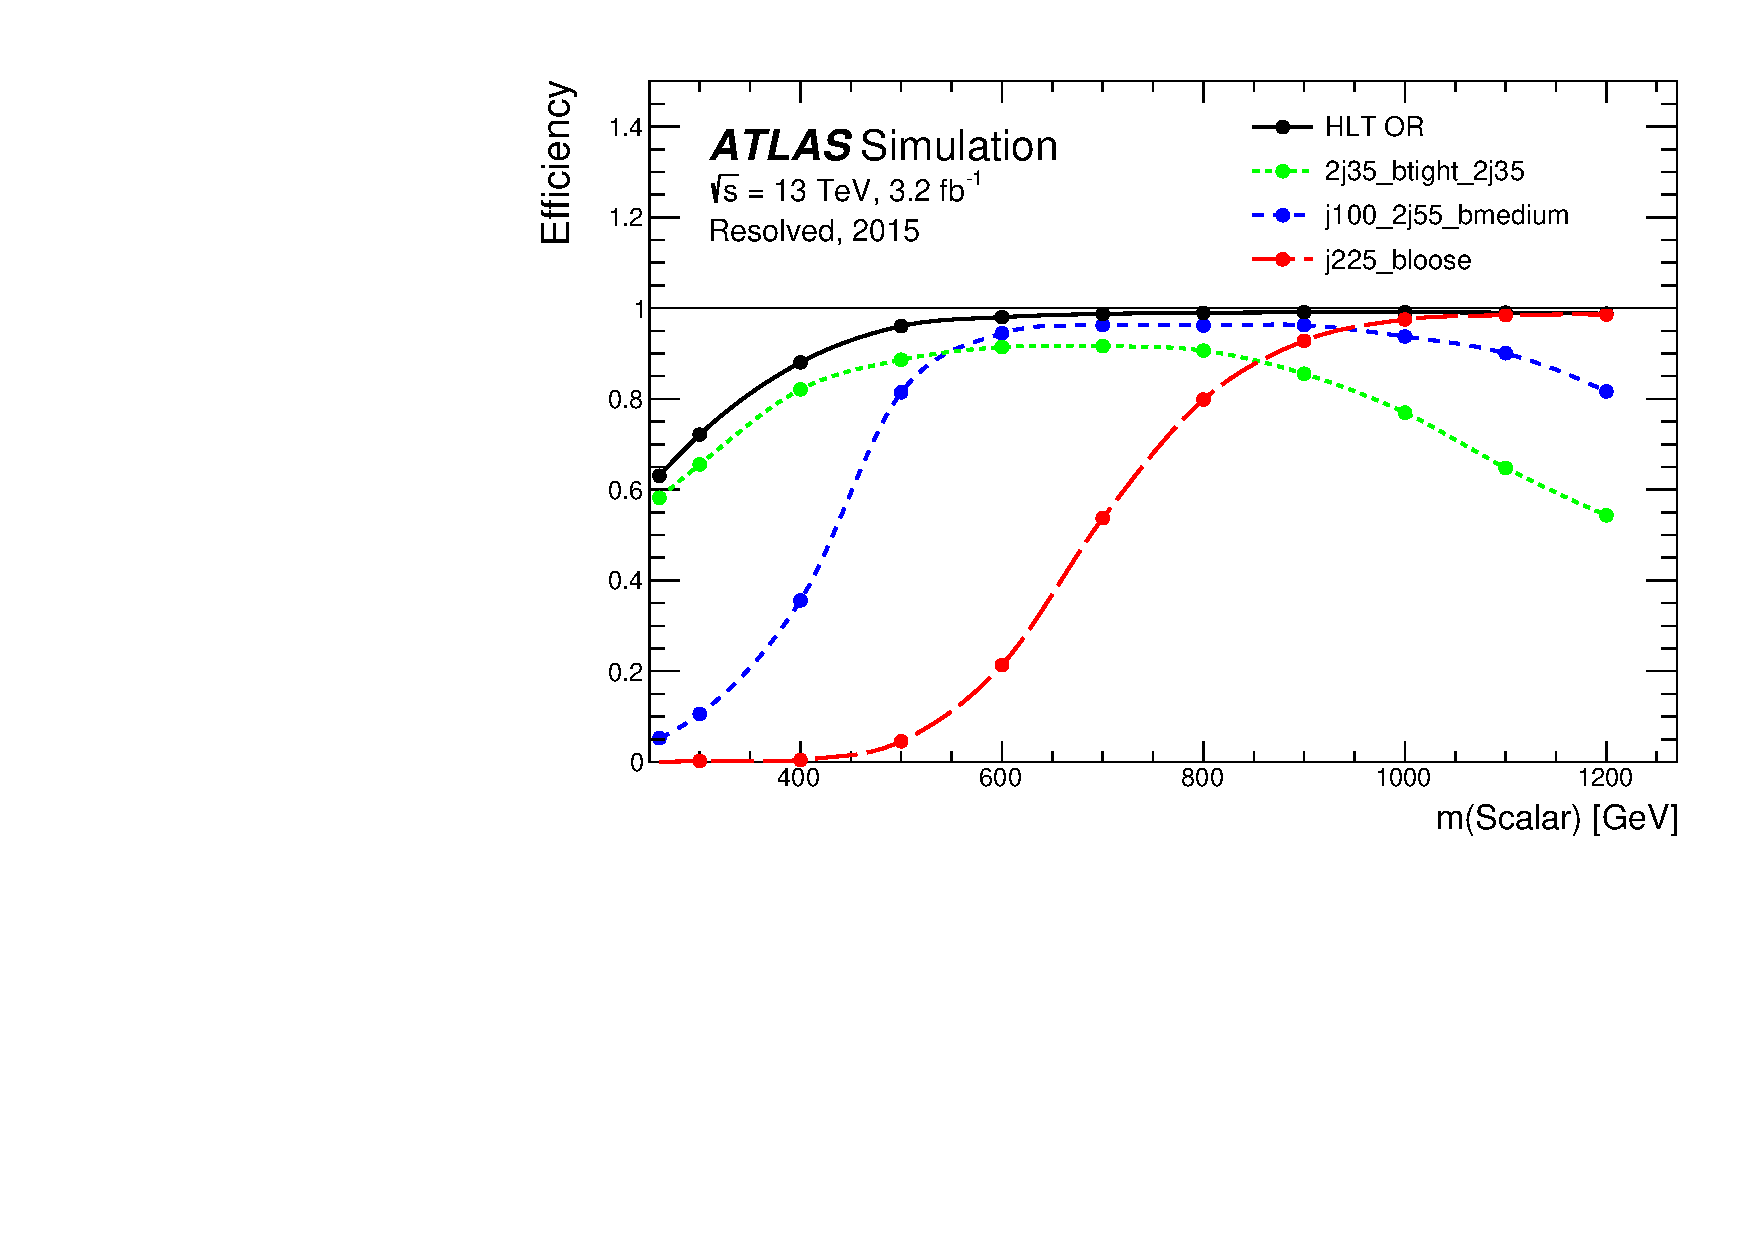
\includegraphics[width=\textwidth,angle=-90]{figures/resolved/extra_plots/trigEff_2015_NWS_passSignal_HLT}
        \caption{2015}
        \label{fig:data_restrig_2015}
    \end{subfigure}
    \quad \quad \quad \quad \quad \quad
    \begin{subfigure}[b]{0.28\textwidth}
        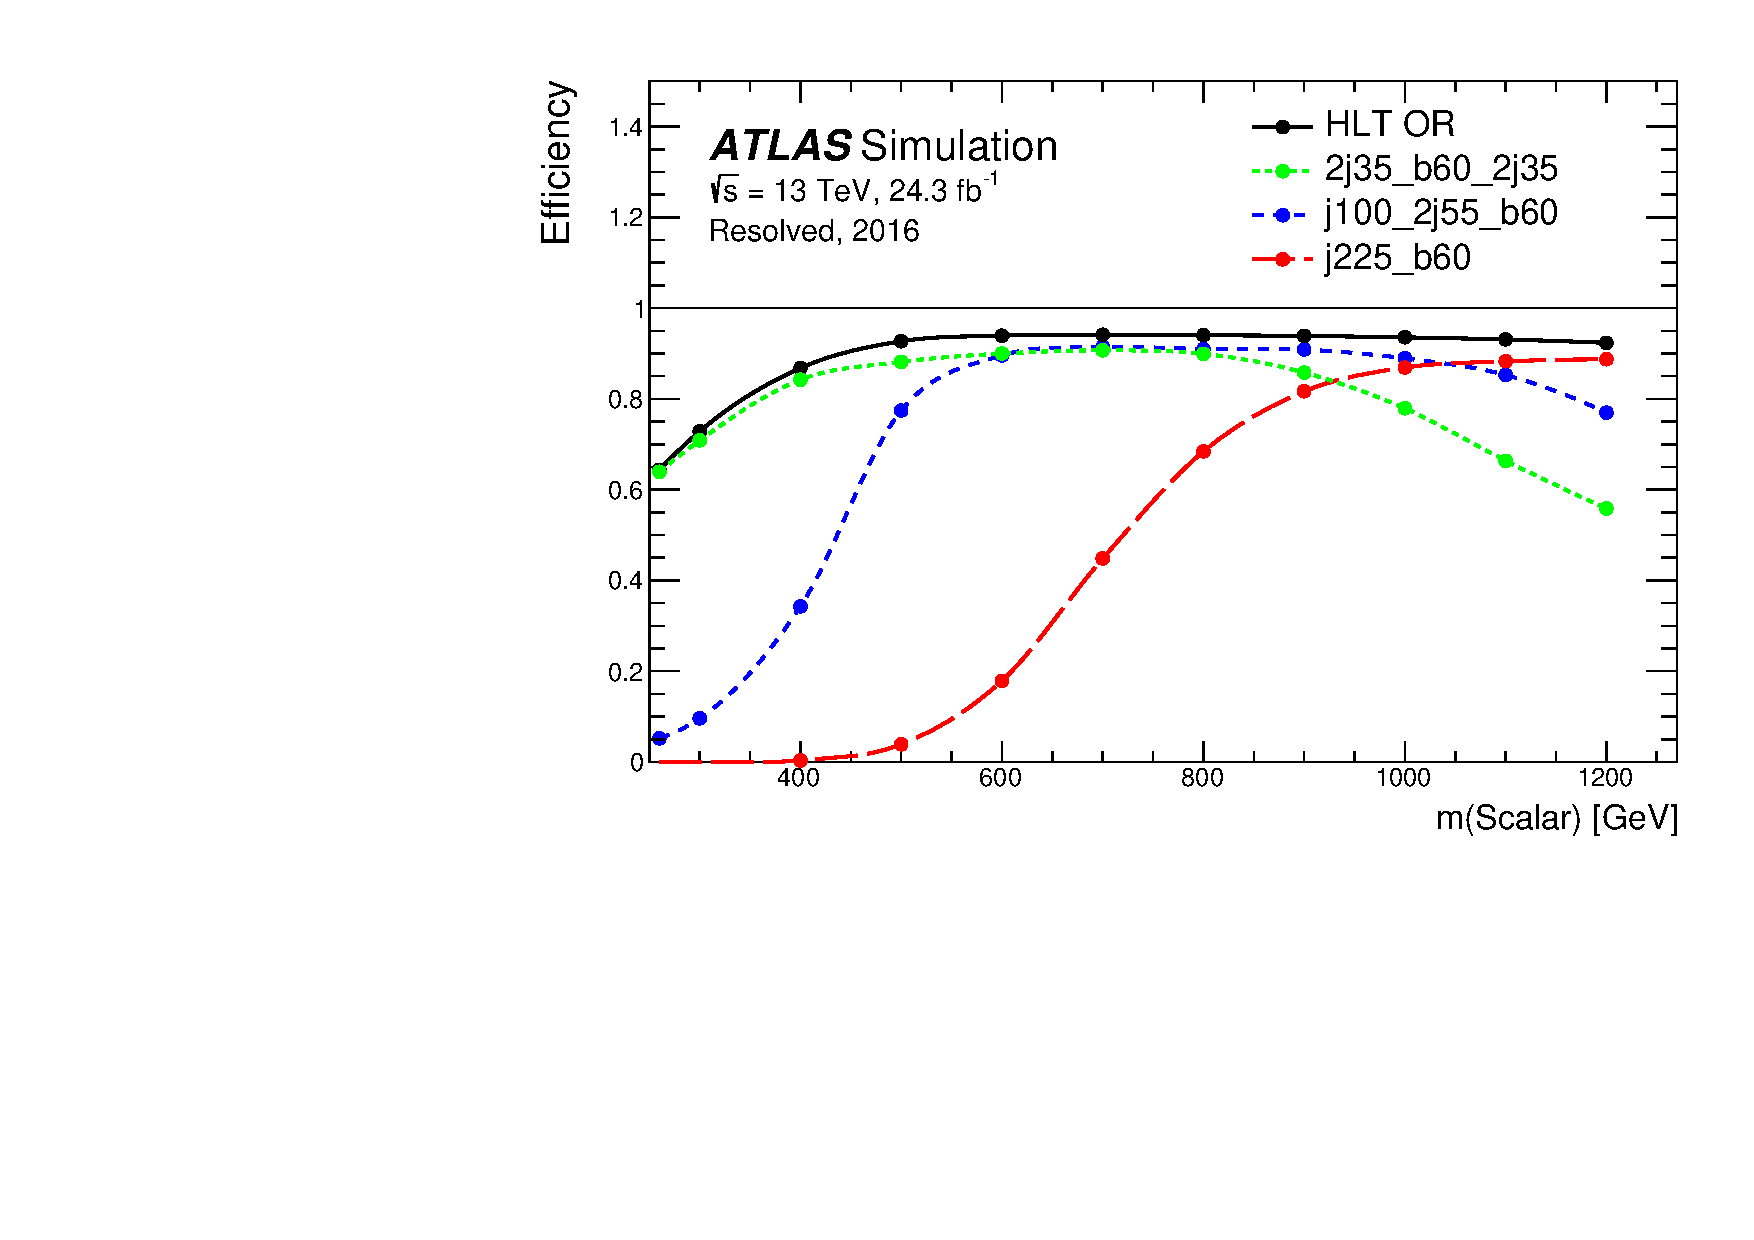
\includegraphics[width=\textwidth,angle=-90]{figures/resolved/extra_plots/trigEff_2016_NWS_passSignal_HLT}
        \caption{2016}
        \label{fig:data_restrig_2015}
    \end{subfigure}
\caption{Trigger efficiencies following the full resolved analysis selection as a function of the resonance signal mass. The efficiencies of the triggers used in 2015 and 2016 are shown. In both graphs, the green line shows the efficiency of the ``2b4j'' trigger; the blue line represents the ``2b3j'' trigger; the red line represents the ``1b1j'' trigger. The 2016 triggers are less efficient due to a bug in the online primary vertex reconstruction.}
\label{fig:data_restrig}
\end{figure}

\paragraph{}
During 2016 data-taking, a fraction of the data was affected by a bug.
The movement of the beam spot was not accounted for in the on-line vertex reconstruction.
This reduced the efficiency of the algorithms used to identify $b$-jets.
That fraction of data is not used and this reduces the integrated luminosity of the 2016 dataset for the resolved analysis to $24.3$ \ifb.

\paragraph{}
In the boosted analysis, events were selected from the 2015 dataset using a trigger that required a single anti-$k_t$ jet with radius parameter $R=1.0$ and with \pt~$>360$~\GeV. In 2016, a similar trigger was used but with a higher threshold of \pt~$>420$~\GeV. The efficiency of these triggers is 100\% for simulated signals passing the jet requirements as described later, so the 2015 and 2016 datasets were combined into one dataset. 

\paragraph{}
The data is further skimmed into the Derived Analysis Object Data (DAOD). The ATLAS off-line software 20.7.8.7 derivation cache is used, with version $p$-tags \textit{p2950}. The boosted slimming keeps events with at least two large-\R jets with \pt~$>200$ \GeV. The final input data file has name format: $dataYR\_13TeV.periodPR.physics\_Main.PhysCont.DAOD\_EXOT8.grpYR\_v01\_p2950$, where YR is $15$ and PR is DEFGHJ for 2015 data, and YR is $16$ and PR is ABCDEFGIKL for 2016 data.


\section{MC}
\paragraph{}
All Monte Carlo (MC) samples used in this analysis are produced with full simulation.
For all simulated samples, charm-hadron and bottom-hadron decays were handled by {\textsc{EvtGen}} 1.2.0~\cite{EvtGen}. 
To simulate the impact of multiple low momentum $pp$ interactions that occur within the same or nearby bunch crossings, minimum-bias events generated with \pythia~8~\cite{Sjostrand:2006za} using the A2 set of tuned parameters~\cite{MC12AU2} were overlaid on the hard-scatter event.
This pile-up effect is simulated with a $\mu$ of $25$.
Although this is different from the pile-up level in data, it has little effect on the analysis and the pile-up reweighting is not adopted.
%https://twiki.cern.ch/twiki/bin/view/AtlasProtected/AtlasProductionGroupMC15c#Pileup_for_samples_with_small_nu
The detector response was simulated with GEANT~4~\cite{Agostinelli:2002hh, Aad:2010ah} and the events were processed with the same reconstruction software as that used for the data.  
Simulated data samples from the ATLAS MC15c campaign are be used, corresponding to $p$-tags \textit{p2952-p2949}.

\section{Signal}
\paragraph{}
In all signal samples, the mass of the Higgs boson ($m_H$) was set to 125~\GeV. 
The signal MC contains truth information, such as the two Higgs and the b quark four-momenta before detector interactions. 
This enables a $\Delta R$ truth matching between the reconstructed objects and the Higgs.

\paragraph{}
SM non-resonant production of Higgs boson pairs via the gluon--gluon fusion process was simulated at NLO with \texttt{MG5\_aMC@NLO}, using form factors for the top-quark loop from HPAIR~\cite{PhysRevD.58.115012, Plehn199646}. 
The simulated events are reweighted to reproduce the \mhh~ spectrum obtained~\cite{Borowka:2016ehy, Borowka:2016ypz}. 
This spectrum is calculated at NLO in QCD while fully accounting for the top-quark mass. 
Interference effects between di-Higgs resonant production and SM non-resonant di-Higgs production are not included in the simulated samples. 
%The cross section times branching ratio to the \fourb\ final state is $11.3^{+0.9}_{-1.0}$~fb~{\cite{Borowka:2016ehy}.
%The uncertainty includes the effects due to renormalization and factorization scales, PDF set, $\alpha_{\mathrm{S}}$, and the \hbb\ branching ratio. 

\paragraph{}
Signal \Gtohhb\ events were generated at leading order (LO) with \texttt{MG5\_aMC@NLO}~2.2.2~\cite{MGaMCatNLO} interfaced with \pythia~8.186 for parton-showering, hadronization and underlying-event simulation. 
The NNPDF2.3 LO parton distribution function (PDF) set~\cite{Ball:2012cx} was used for both \texttt{MG5\_aMC@NLO} and \pythia. 
The A14 set of tuned underlying-event parameters was used. 
These signal samples were generated with $\kMPl = 1$ or $2$.
Relative to the resonance mass, widths of the graviton signals range from 3\% (at low mass) to 13\% (at the highest mass) for $\kMPl=1$, and $6\%$ to $25\%$ for $\kMPl=2$.
The graviton samples were normalized using fixed cross sections~\cite{carvalho}.

\paragraph{}
Signal 2HDM Scalar \tohhb\ events were generated at LO in QCD with \texttt{MG5\_aMC@NLO}~2.2.3 interfaced with \textsc{Herwig++}~\cite{Bahr:2008pv} for parton-showering, hadronization and simulation of the underlying event. CT10~\cite{Lai:2010vv} PDF sets were used for \texttt{MG5\_aMC@NLO} and CTEQ6L1~\cite{cteq6l1} for \textsc{Herwig++}.
The UE-EE-5-CTEQ6L1 set of tuned underlying-event parameters \cite{Seymour:2013qka} was used. 
The scalar signals were generated with a width of $1$~\GeV, which represent generic narrow-width scalar signals. 
Because the width and branching ratios depend on 2HDM parameters, each mass point generated with this fixed width corresponds to a different point in the 2HDM parameter phase space.
%No specific model was considered for computing the scalar signal cross sections.
%For the evaluation of theoretical uncertainties in the signal modeling, samples were produced with variations of the factorization and renormalization scales, PDF sets (following the prescription from Ref.~\cite{pdfs}) and shower generator. For the latter, scalar (spin-2) samples were produced that are interfaced to \PYTHIA~8.186 rather than \textsc{Herwig++} (and vice versa).

\paragraph{}
Resonant signal samples for the scalar and $\kMPl=1$ models were produced in $10$~\GeV\ steps between $260$ and $300$~\GeV, in $100$~\GeV\ steps up to $1600$~\GeV, in $200$~\GeV\ steps up to $2000$~\GeV, and in $250$~\GeV\ steps up to $3000$~\GeV. Signal samples for the $\kMPl=2$ model were produced with the same spacings but omitting the masses of $270$~\GeV, $290$~\GeV\ and $2750$~\GeV\ due to the larger generated width. Unless specified, the MC signal sample used as benchmark is $\kMPl=1$ \Grav, due to its width is medium among the three signal models.

\subsection{Backgrounds}
\paragraph{}
A very small fraction of the background arises from $Z$ + jets events. The $Z$+jets sample was generated using \pythia~8.186 with the NNPDF2.3 LO PDF set.

\paragraph{}
The \ttbar\ background is modeled using large all-hadronic and non-all-hadronic samples that have both been generated with \powhegbox\ v1~\cite{Alioli:2010xd} using the CT10 PDF set. 
The parton shower, hadronization, and the underlying event were simulated using \pythia~6.428 with the CTEQ6L1 PDF set and the corresponding Perugia 2012 set of tuned underlying-event parameters~\cite{Skands:2010ak}.
The $t$-quark mass in both samples is set to $172.5$ \GeV~.
Higher-order corrections to the \ttbar\ cross section were computed with Top++~2.0~\cite{Czakon:20142930}. These incorporate NNLO corrections in QCD, including re-summation of NNLL soft gluon terms.
The \ttbar\ MC samples are normalized to the NNLO+NLL predicted inclusive \ttbar\ cross-section of
$1821.87$ pb multiplied by the all-hadronic branching ratio of $0.457$ and non-all-hadronic of $0.543$.

\paragraph{}
In order to minimize statistical fluctuations across the dijet invariant mass spectrum, especially for large values of $m_{tt}$, additional \ttbar~ samples are generated in slices of \ttbar~ invariant mass. The cross-section of the \ttbar~ process is normalized to NNLO+NNLL in QCD, as calculated by \textsc{Top++} 2.0. Overlap with the inclusive \ttbar~ samples is removed by a fixed cut on the truth value of $m_{tt}$ at $1100$ \GeV.

\paragraph{}
A \pythia~ dijet sample is used to understand the multi-jet background and characteristics of the event selection. This MC sample is generated without a heavy flavor filter, hence is limited by the total generated number of events, given the high background rejection factors of the analysis selection.











%Data, MC
%!TEX root = ../dissertation.tex
\begin{savequote}[75mm]
You gotta have a swine to show you where the truffles are.
\qauthor{Edward Albee}
\end{savequote}

\chapter{Event Selection}
\label{sec:selection}

\begin{figure}[h!]
  \centering
  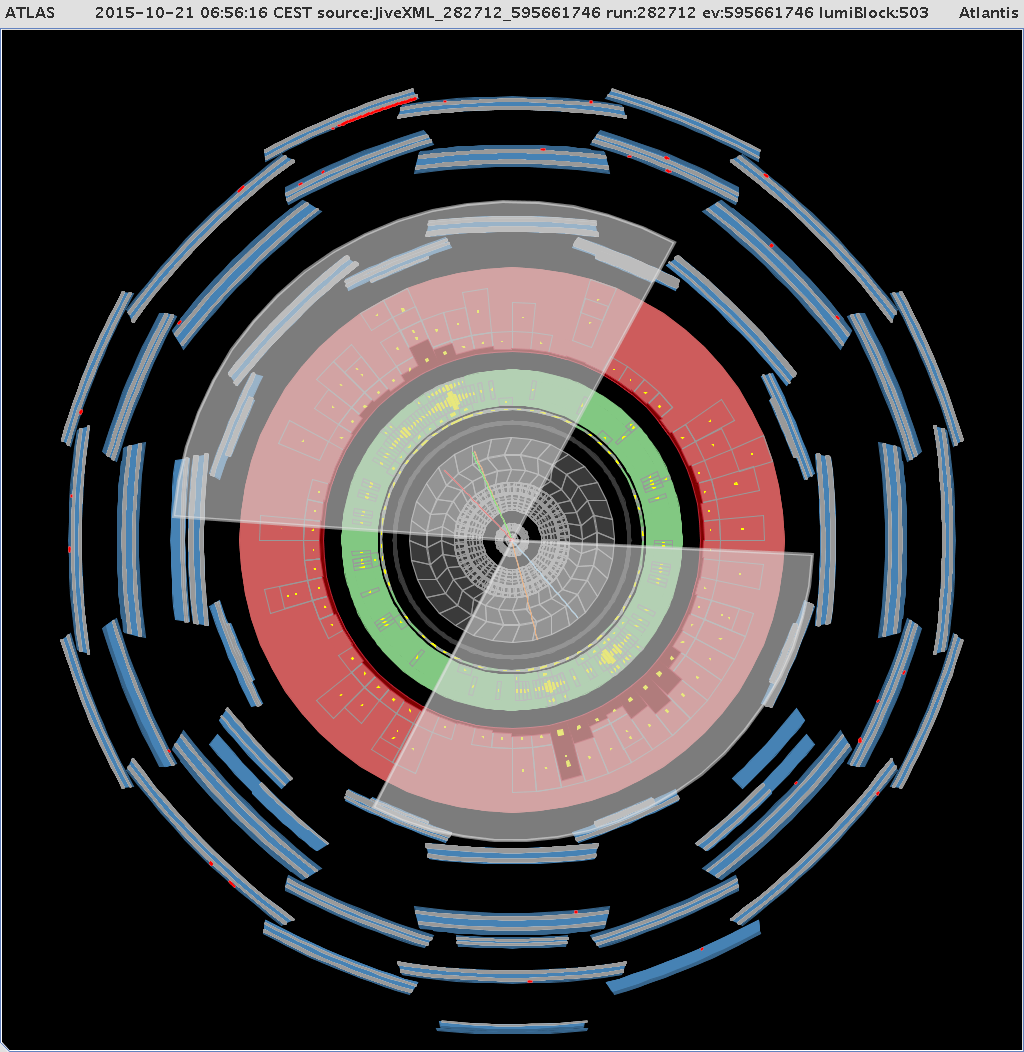
\includegraphics[width=0.7\textwidth]{figures/theory/JiveXML_282712_595661746-YX-2018-04-16-20-50-34}
  \caption{2015 ATLAS boosted di-Higgs event candidate's event display. The data is taken in run 282712, lumiblock 503 and has event number 595661746. ID is in grey, ECAL is in green, HCAL is in red and MS is in blue. Only tracks with \pt $>25$ \GeV are shown. Jets are gray cones, and ID tracks are colored lines in the ID. There are $2b$ tagged tracks within in each of the large-\R jets. The one large-\R jet has $119$ \GeV mass and $543$ \GeV \pt, and the other one has $127$ \GeV mass and $413$ \GeV \pt. The $\Delta R$ between the two large-\R jet is $3.54$ and the invariant mass of the two large-\R jets is $1336$ \GeV. }
  \label{fig:event_display}
\end{figure}

\paragraph{}
An example of \Xtohhb~ boosted event is shown in Figure~\ref{fig:event_display}. This chapter explains how this event is selected as a \Xtohhb~ candidate.

\section{Data Cleaning}
\label{evt-sel:cleaning}
\paragraph{}
The following data cleaning requirements are made:
\begin{itemize}
\item Events with problems in SCT/TileCal/LAr are removed.
%\item Events that are affected by the recovery procedure for single event upsets in the SCT are removed.
\item Events that fail the jet cleaning procedure are removed. This is designed to exclude jets caused by detector noise, non-collision backgrounds and cosmic rays. 
\item Incomplete events are removed.
\end{itemize}
% \paragraph{}
% Jets with $p_T<60$~\GeV\, $|\eta|<2.4$, and with a large fraction of their energy arising from pile-up interactions are suppressed using tracking information. 
% Events that pass a ``medium'' jet vertex tagger working point, corresponding to a 92\% efficiency for jets at the EM scale with $20<p_T<60$~\GeV, are retained in the analysis. 
% Quality criteria are applied to the jets, and events with jets consistent with noise in the calorimeter or non-collision backgrounds are vetoed~\cite{jetcleanATLAS}.
\paragraph{}
The analysis also runs over the debug stream, which contains events recorded that couln't be reconstructed online due to CPU time constrains. No event passing the full signal selection is found.


%%%%%%%%%%%%%%%%%%%%%%%%%%%%%%%%%%%%%%%%%%%%%%%%%%%%%%%%%%%%%%%%%%%%%%%%%%%%%%%%%%%%%%%%%%
\section{Trigger}
\label{evt-sel:trig}
\paragraph{}
%See \href{https://arxiv.org/pdf/1611.09661.pdf}{6.4.3} 
Events in data and MC are required to pass the lowest unprescaled large-\R jet trigger: \\
\verb|HLT_j360_a10_lcw| in 2015 and \verb|HLT_j420_a10_lcw| in 2016. 
The triggered jets are topo-cluster jets with local calibration weights and pile-up subtraction.
They are seeded by the lowest unprescaled L1 jet trigger, \texttt{L1\_J100}. 
LCW cluster trigger is chosen, because the other option, reclusted large-\R jet trigger, has slower turn-on in multi-jet events. 
Other options such as the lowest unprescaled HT trigger, \verb|HLT_ht1000|, has a much slower turn-on compared to large-\R jet triggers.
Another trigger option is \verb|HLT_4j100|, but because of the boosted jets merging, the trigger efficiency decreases rapidly as the signal mass increases. 
The results are shown in Figure~\ref{fig:boosted-trigger-HLT}.

\begin{figure}[htbp!]
\begin{center}
  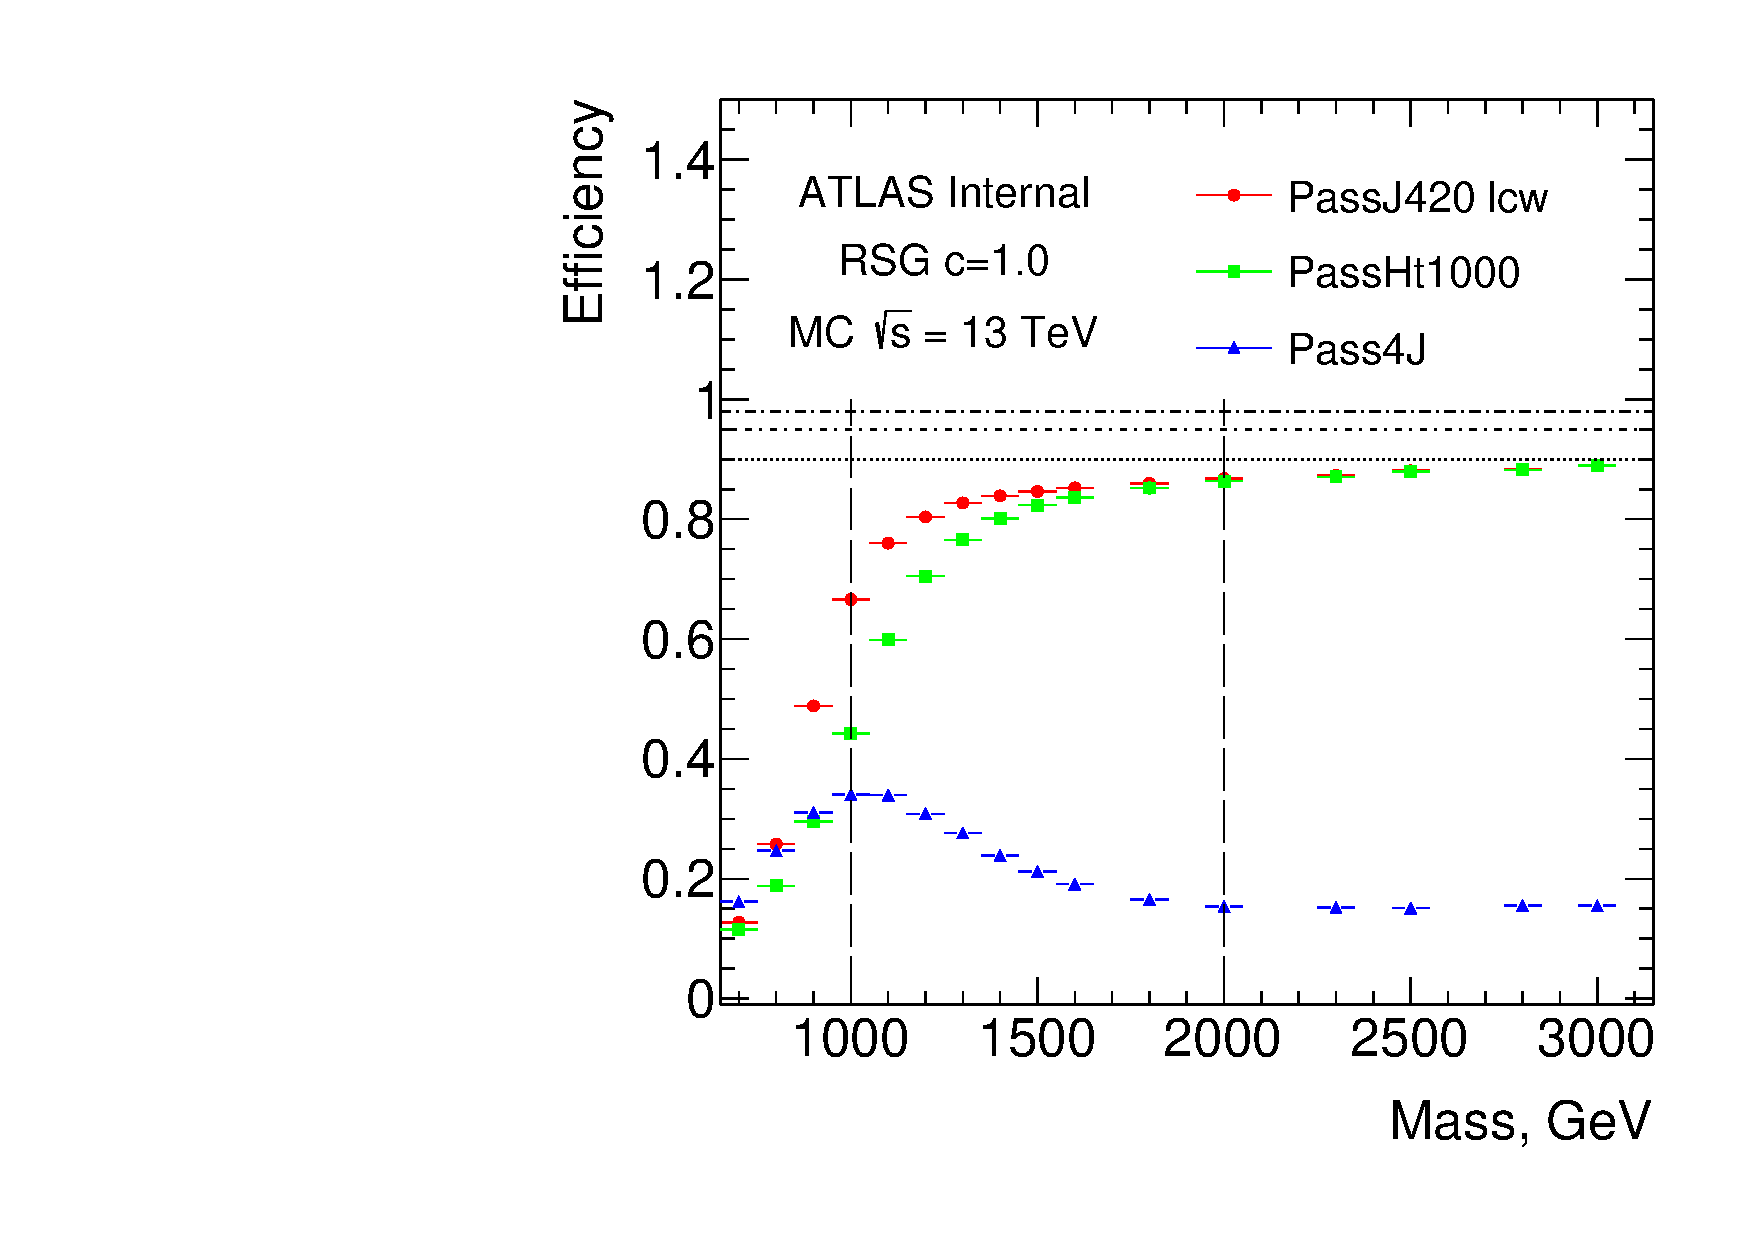
\includegraphics[width=0.45\textwidth,angle=-90]{figures/boosted/Trigger/app_trig_b77_Efficiency_PreSel.pdf}
  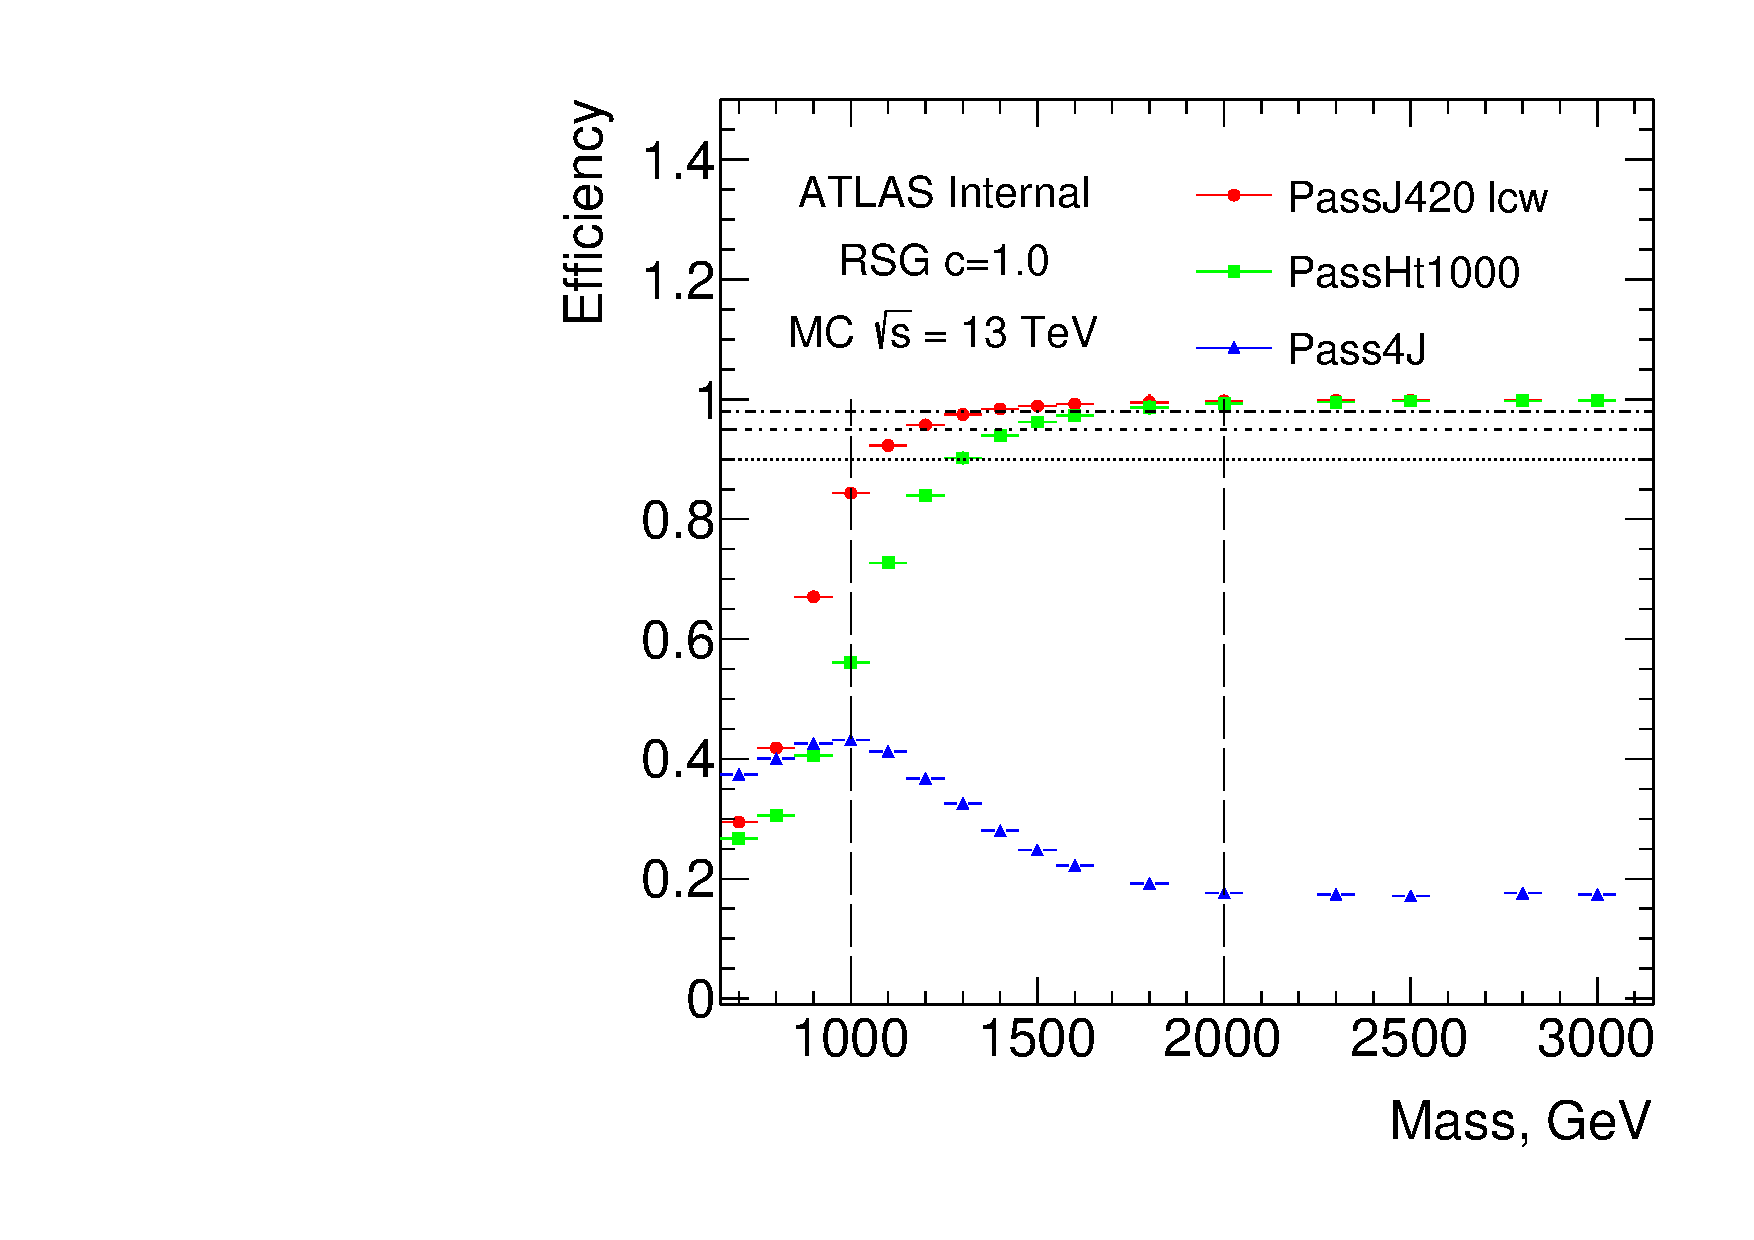
\includegraphics[width=0.45\textwidth,angle=-90]{figures/boosted/Trigger/app_trig_b77_Efficiency_All.pdf}
  %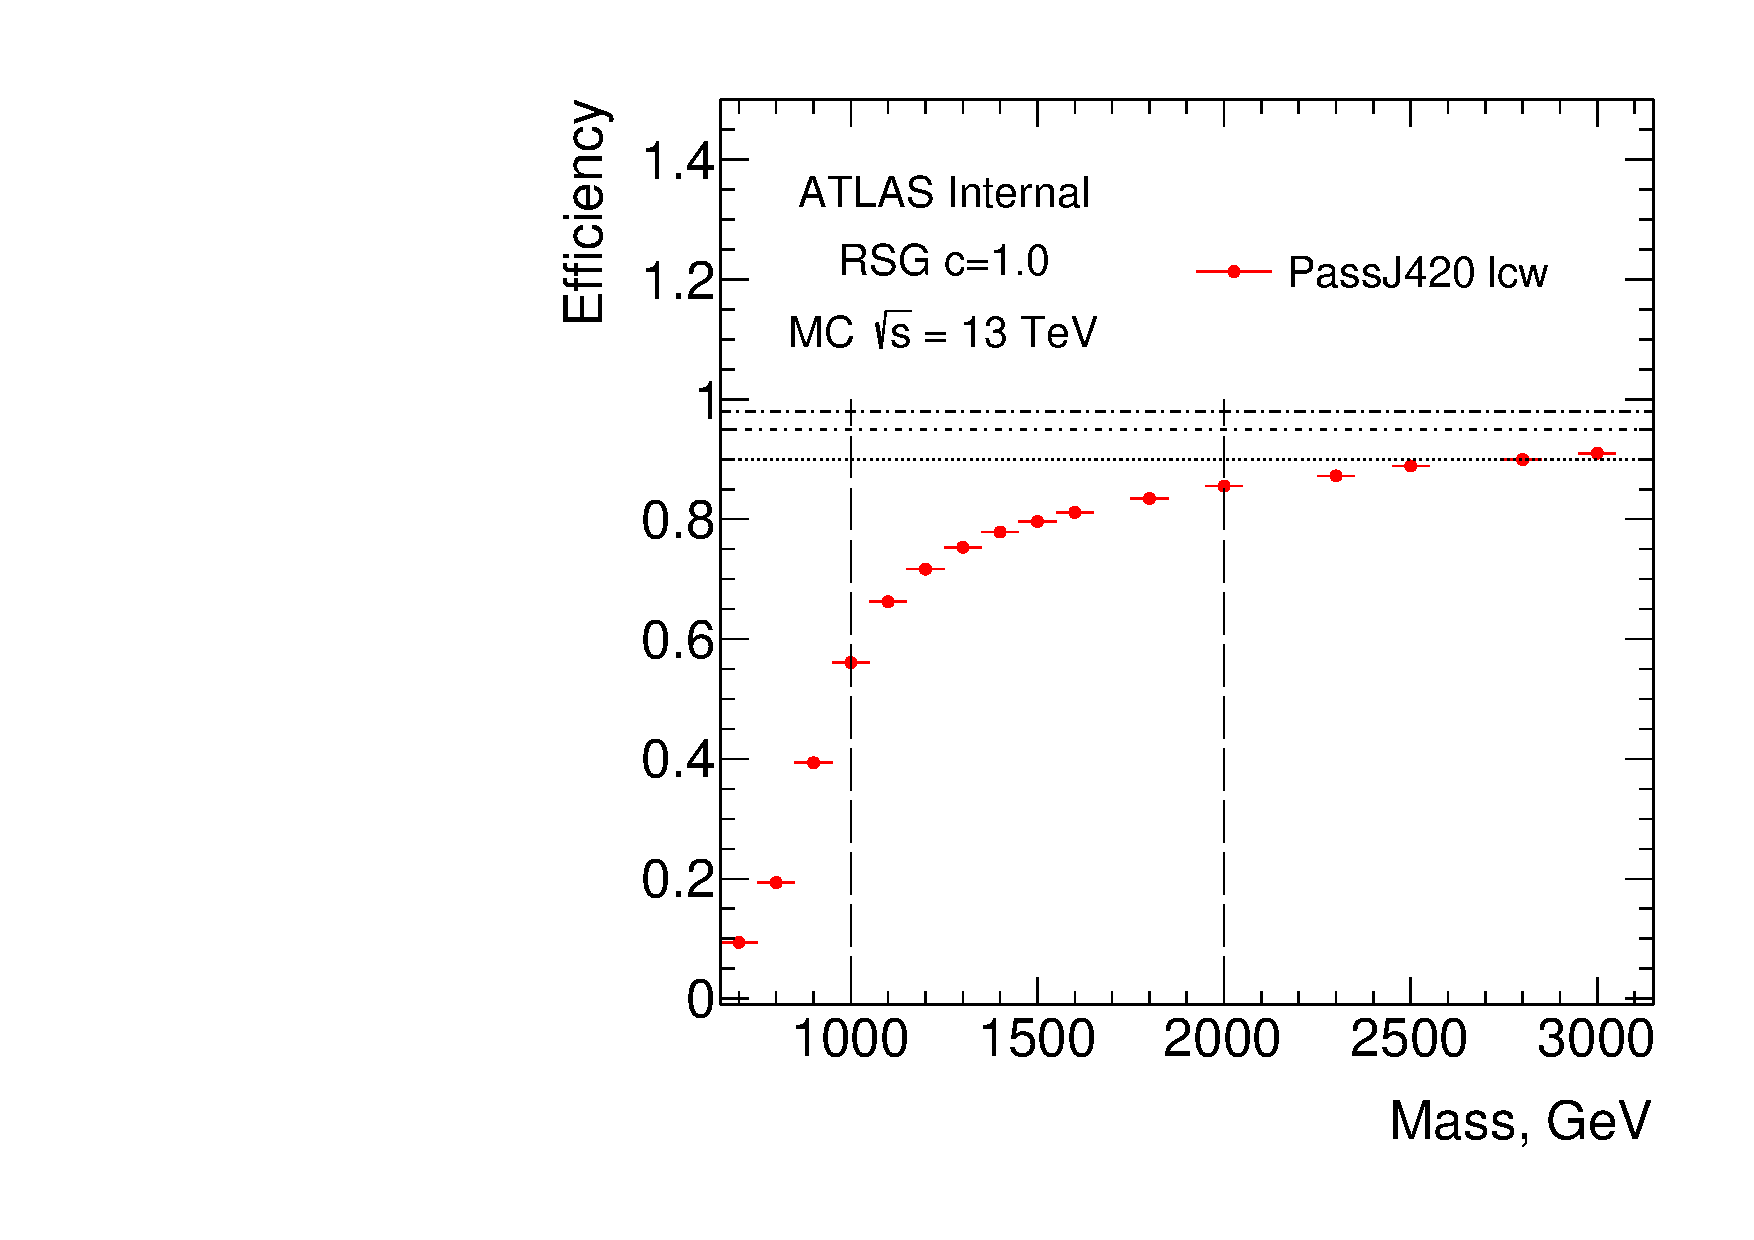
\includegraphics[width=0.45\textwidth,angle=-90]{figures/boosted/Trigger/trig_Moriond_Efficiency_PreSel.pdf}
  %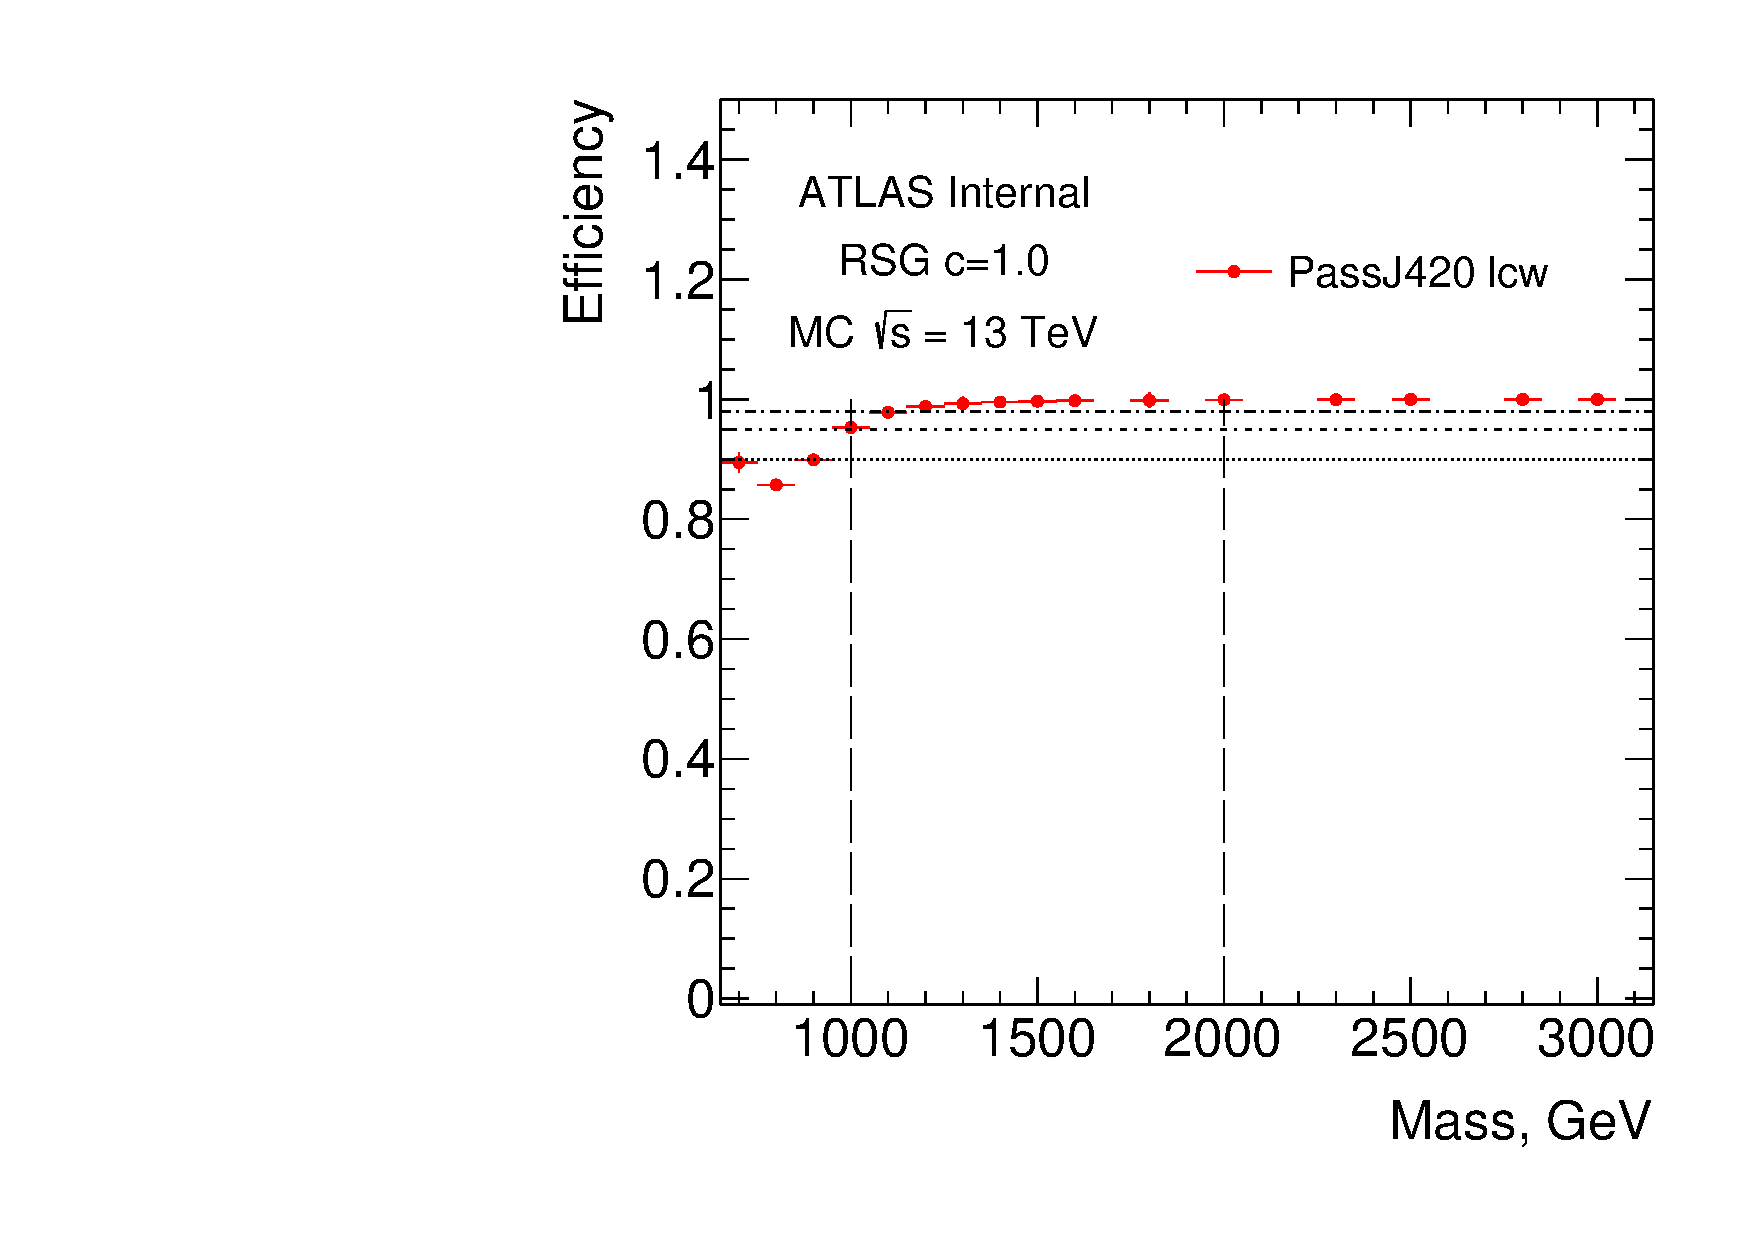
\includegraphics[width=0.45\textwidth,angle=-90]{figures/boosted/Trigger/trig_Moriond_Efficiency_All.pdf}
  \caption{Different trigger efficiencies as a function of the signal resonance mass with respect to all events with no selection (left) and with respect to events passing the two large-\R jets \pt $> 400$ \GeV~ and leading/subleading jet \pt $> 250$ \GeV (right). For $1.4$ \TeV~ signal, the trigger efficiency is about $98\%$.}
  \label{fig:boosted-trigger-HLT}
\end{center}
\end{figure}

\paragraph{}
The selected large-\R triggers are found to have $>98\%$ efficiency for signals with mass above 1400 \GeV.
% with the requirement that the event has two large-\R jets that satisfy the \pt requirements: leading jet \pt $> 400$ \GeV, and subleading jet leading jet \pt $> 250$ \GeV. 
The trigger turn-on curve in 2015 and 2016 data, as a function of leading jet \pt, is shown in Figure~\ref{fig:boosted-trigger-HLT-turnon}.
\begin{figure}[htbp!]
\begin{center}
  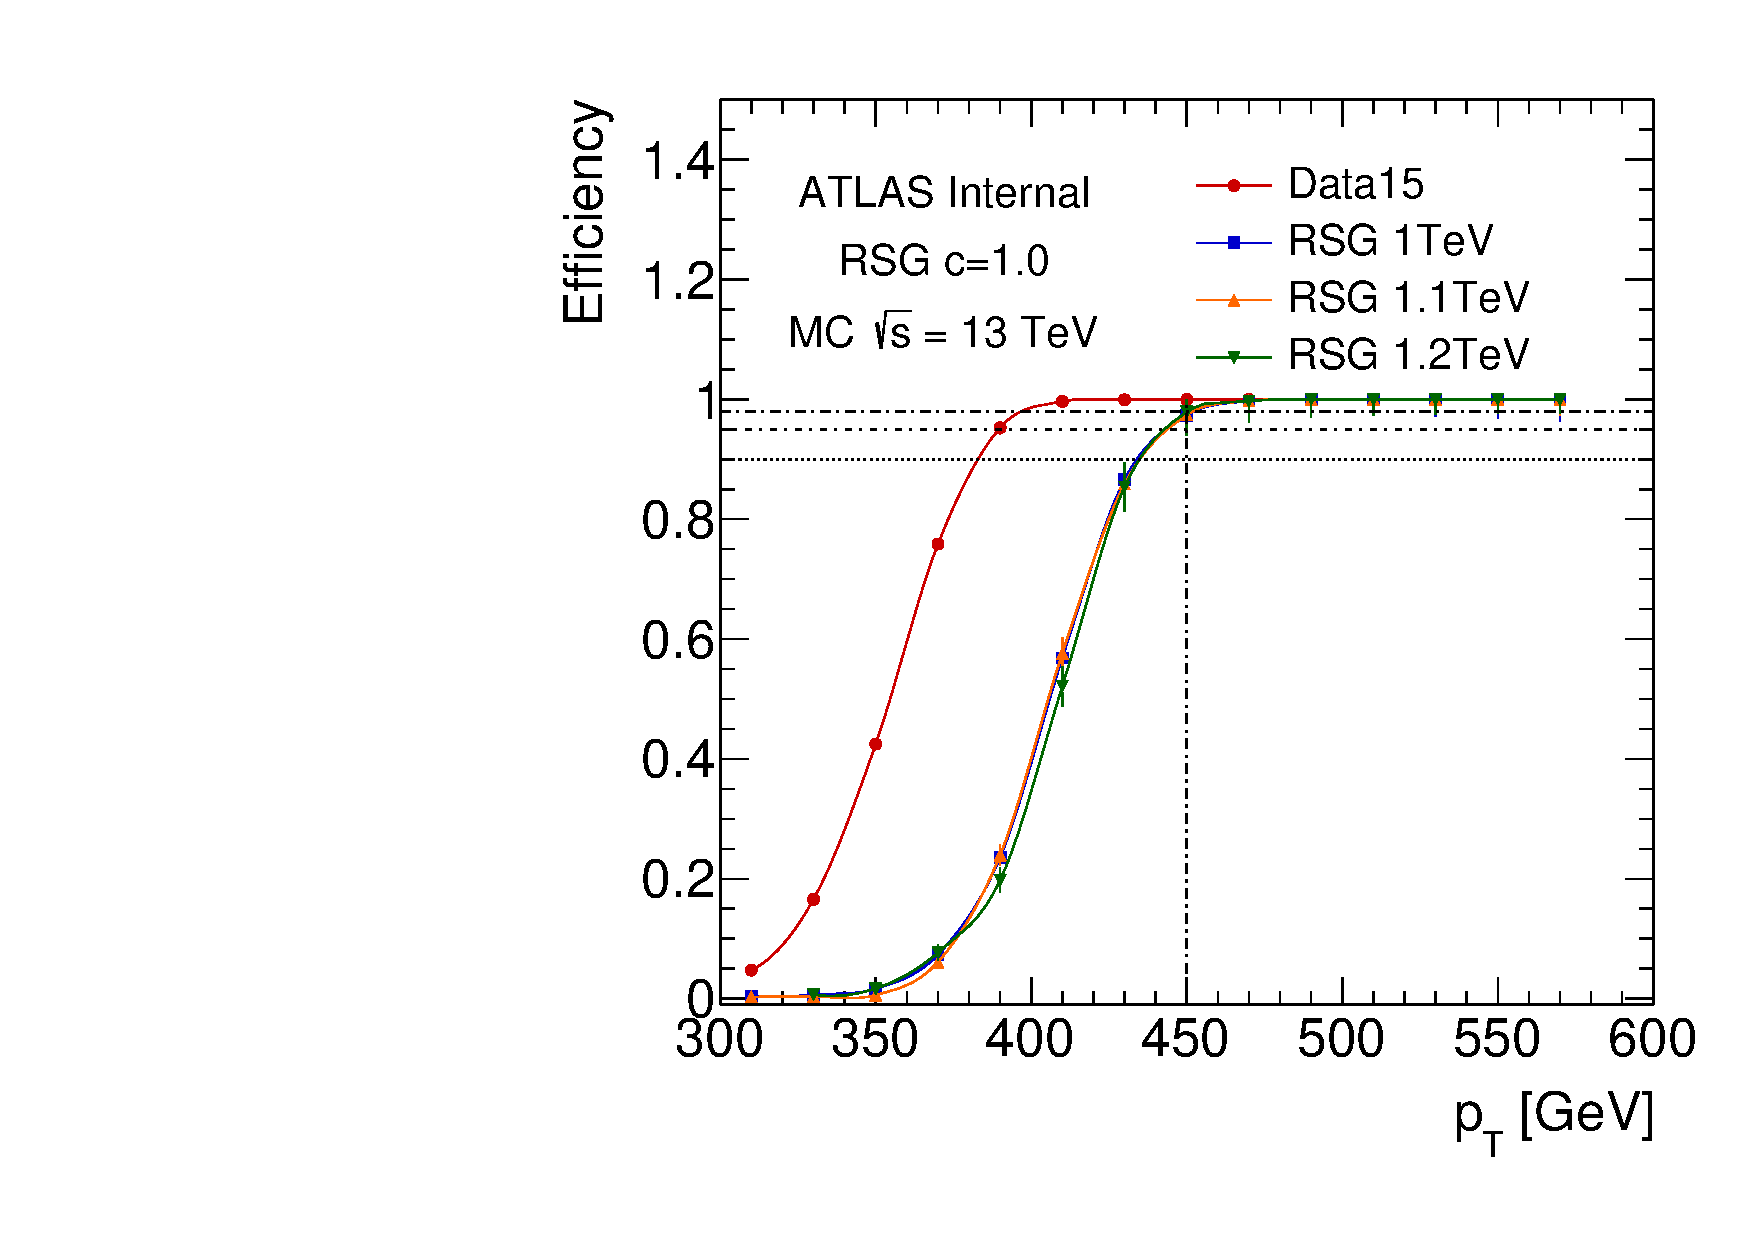
\includegraphics[width=0.45\textwidth,angle=-90]{figures/boosted/Trigger/trig_15_b77_pT_Efficiency.pdf}
  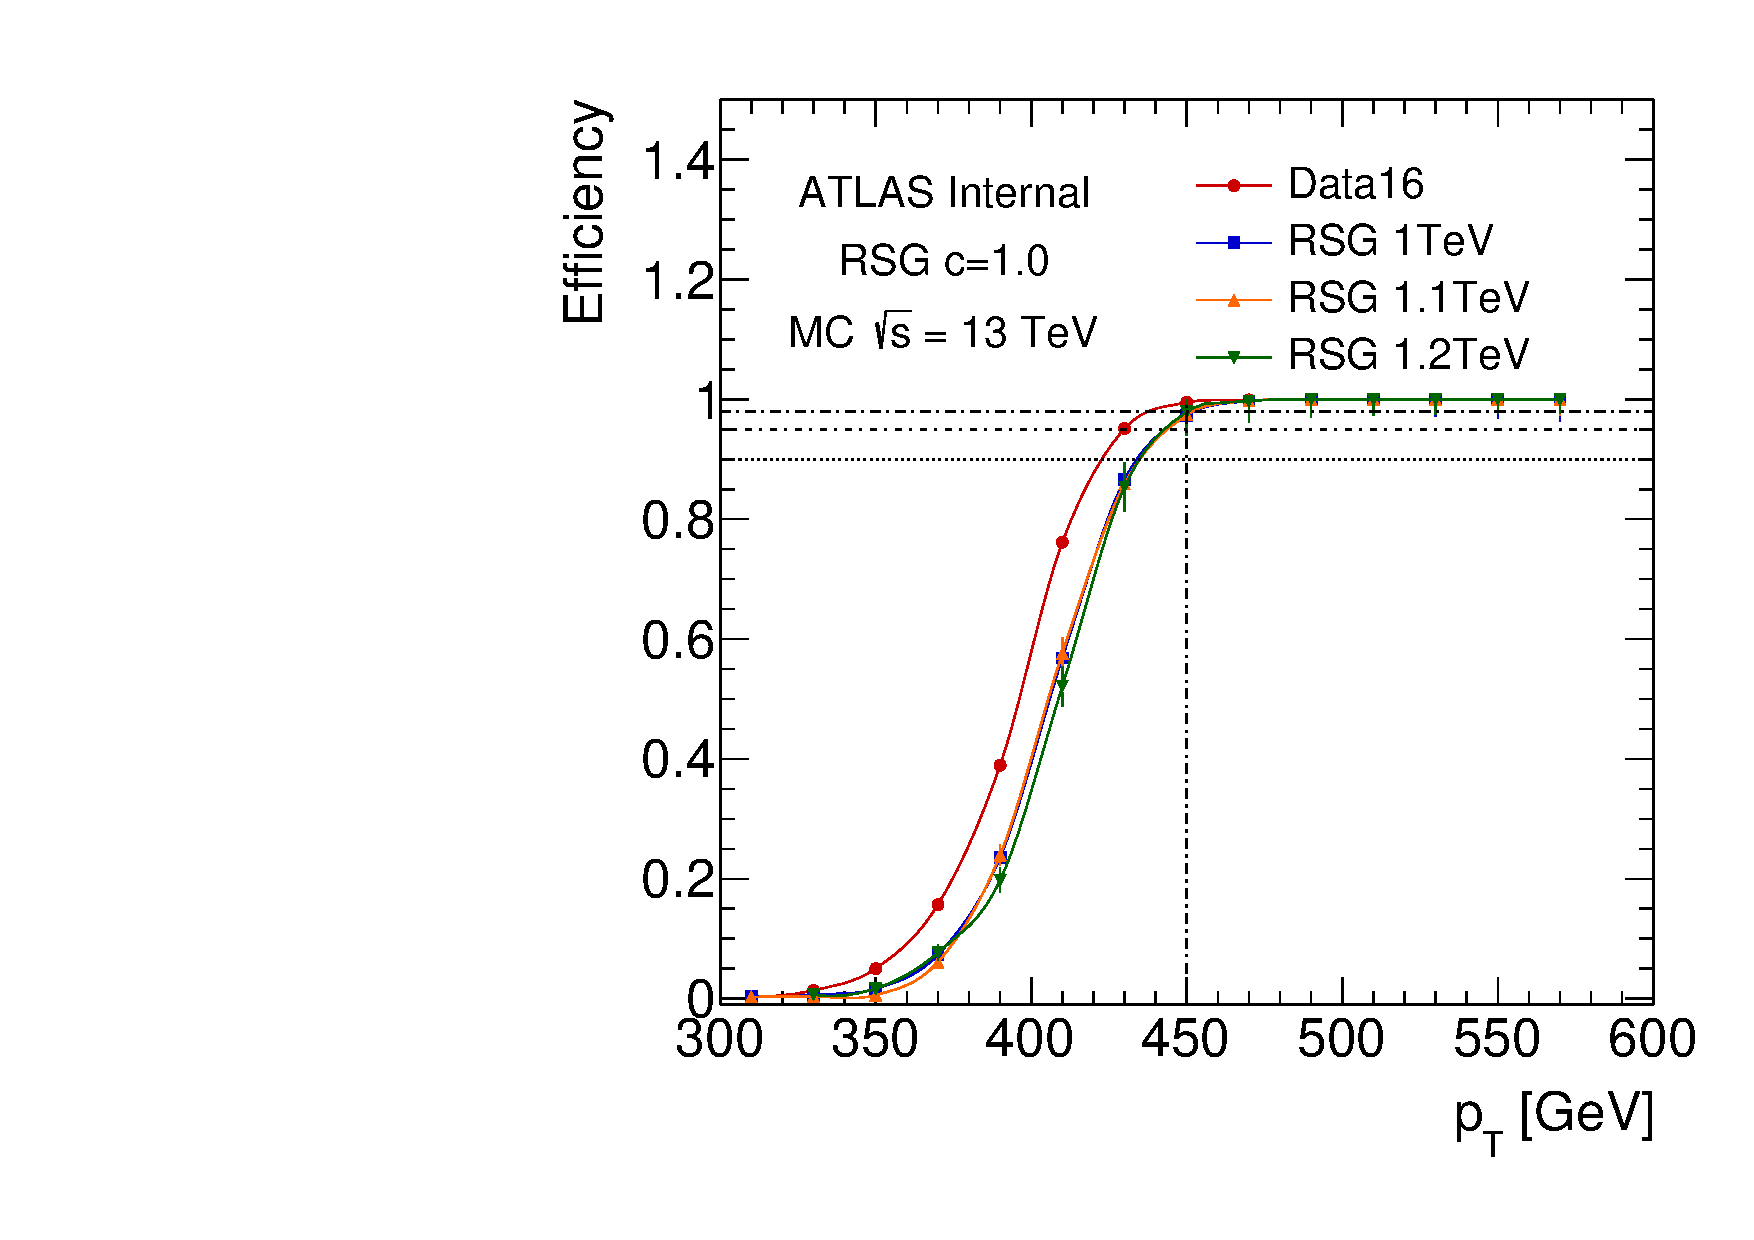
\includegraphics[width=0.45\textwidth,angle=-90]{figures/boosted/Trigger/trig_16_b77_pT_Efficiency.pdf}
  \caption{Large-$R$ jet trigger efficiencies, defined as the fraction of events fired trigger with a given highest large-\R jet \pt, measured in 2015 Data (\texttt{HLT\_j360\_a10\_lcw}, left) and 2016 Data (\texttt{HLT\_j420\_a10\_lcw}, right) and MC.}
  \label{fig:boosted-trigger-HLT-turnon}
\end{center}
\end{figure}


%%%%%%%%%%%%%%%%%%%%%%%%%%%%%%%%%%%%%%%%%%%%%%%%%%%%%%%%%%%%%%%%%%%%%%%%%%%%%%%%%%%%%%%%%%
\section{Object Selection}
\paragraph{}
The specific physics objects used in the boosted analysis are described in previous sections and reiterated in Table~\ref{tab:boosted-objects}.

\begin{table}[bhp]
\caption{Physics objects and their technical names in the boosted analysis.} %%%
\begin{center}
\begin{tabular}{c|c}
  object & technical name \\
  \hline
  large-$R$ calorimeter jets & AntiKt10LCTopoTrimmedPtFrac5SmallR20Jets \\
  small-$R$ track jets       & AntiKt2PV0TrackJets \\
  b-tagging                  & on track jets, MV2c10, $70\%$ b-tagging wp \\
\end{tabular}
\label{tab:boosted-objects}
\end{center}
\end{table}

\paragraph{}
Each event must have at least two high momentum large-\R jets, each with at least one ghost associated track jets for $b$-tagging.
They are sorted by \pt, and the highest \pt~ one is named as the leading large-\R jet, or the leading Higgs Candidate.
The second highest \pt~ large-\R jet is the subleading large-\R jet, or the subleading Higgs Candidate.
The large-\R jets are required to have \pt $> 250$ \GeV~, $|\eta| < 2$ to guarantee a good overlap with the tracking acceptance, and mass $> 50$ \GeV~ to avoid oversized derivations.
The leading large-\R jet is also required to have \pt $> 450$ \GeV~ to be above the trigger turn on threshold.
Only the leading and subleading large-\R jets are considered in the rest of this thesis.
This selection is $\sim 95\%$ efficient for $1.2$ \TeV signals, as shown in Figure~\ref{fig:truth-Higgs-largeRjet}. 
$R = 1.0$ ensures that the two $b$ quarks and their decay products are very likely to be contained within the large-\R jet, as shown in Figure~\ref{fig:truth-HbdR}. 

\begin{figure}[htbp!]
	\begin{center}
	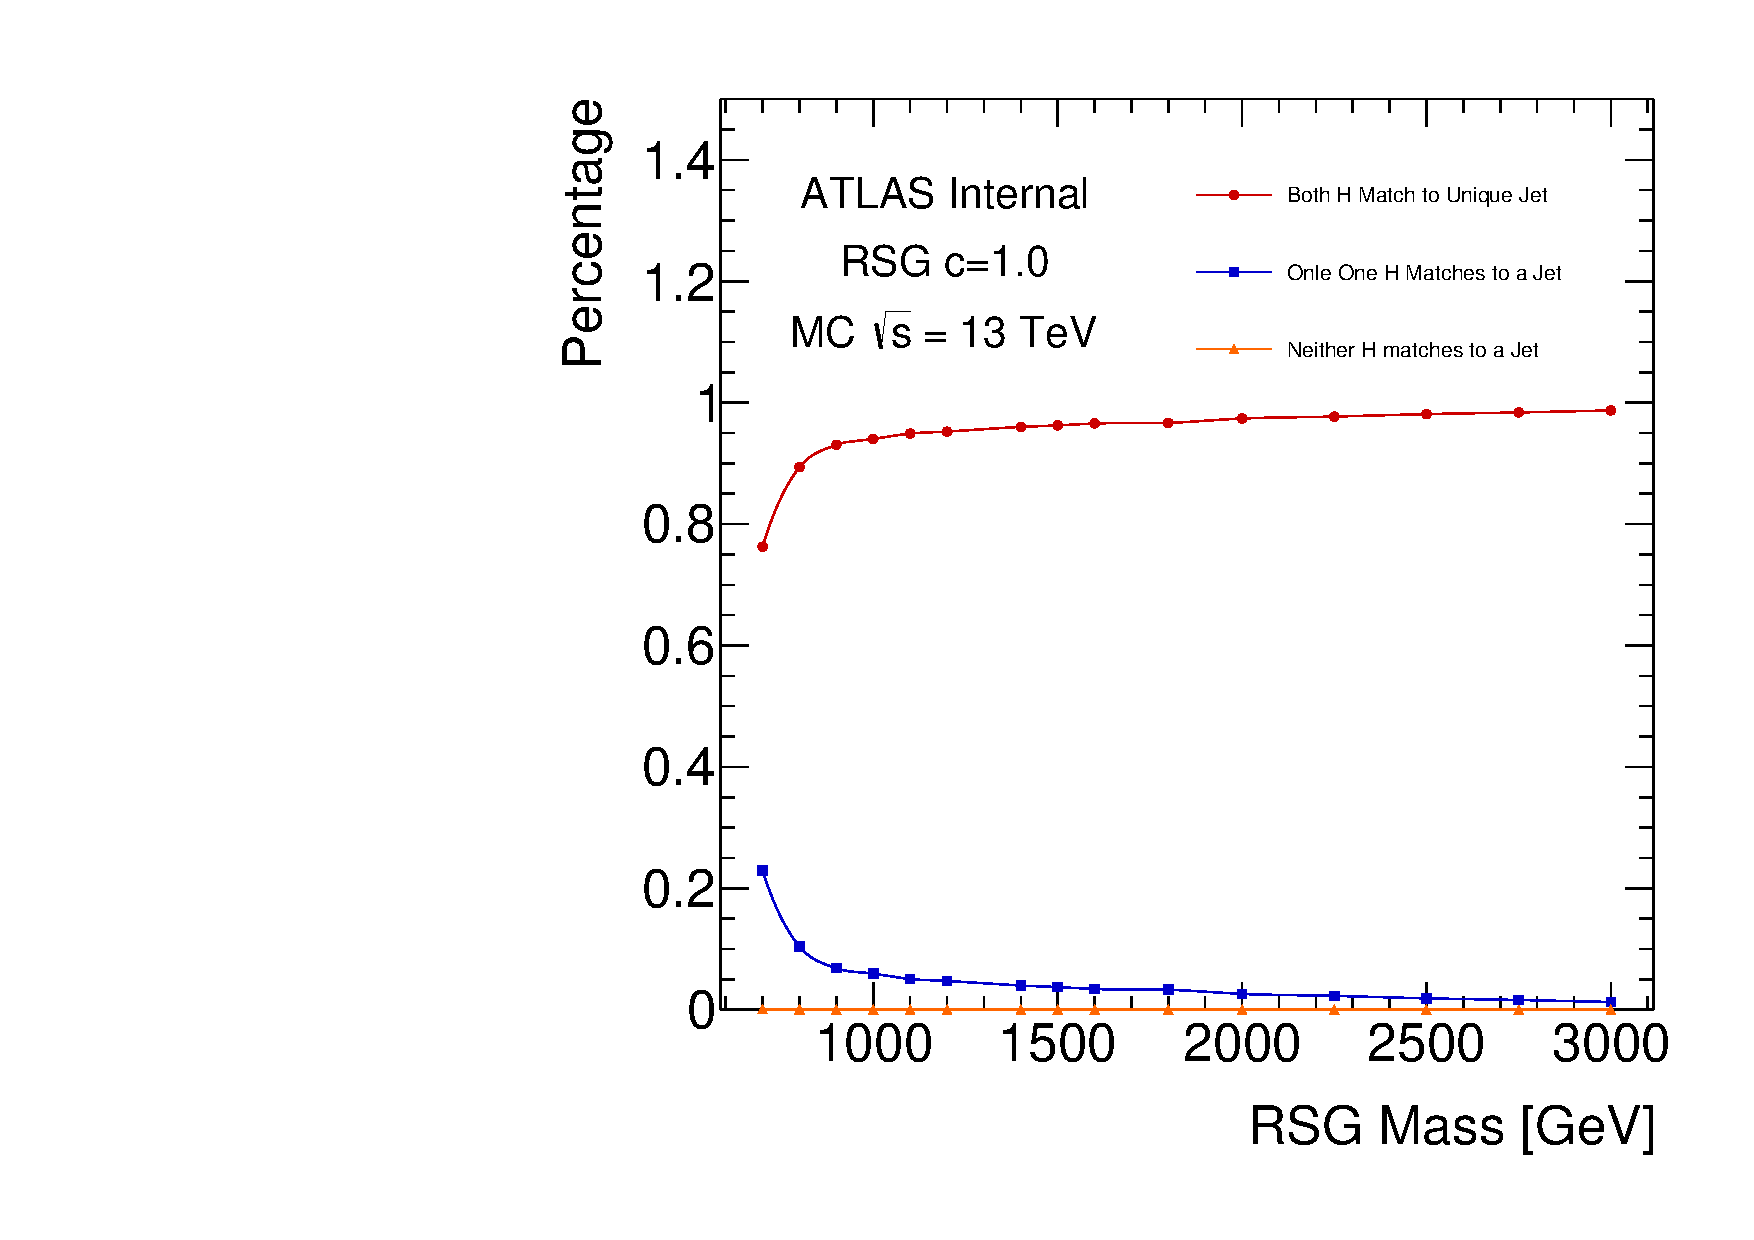
\includegraphics[scale=.45,angle=-90]{figures/boosted/Truth/truth_higgs-matching.pdf}
	\caption{Percentages of truth Higgs to large-\R jet $\Delta R<1.0$ matching as a function of \Grav~ mass. Both Higgs almost never match to the same large-\R jet.}
	\label{fig:truth-Higgs-largeRjet}
\end{center}
\end{figure}

\begin{figure}[htbp!]
\begin{center}
  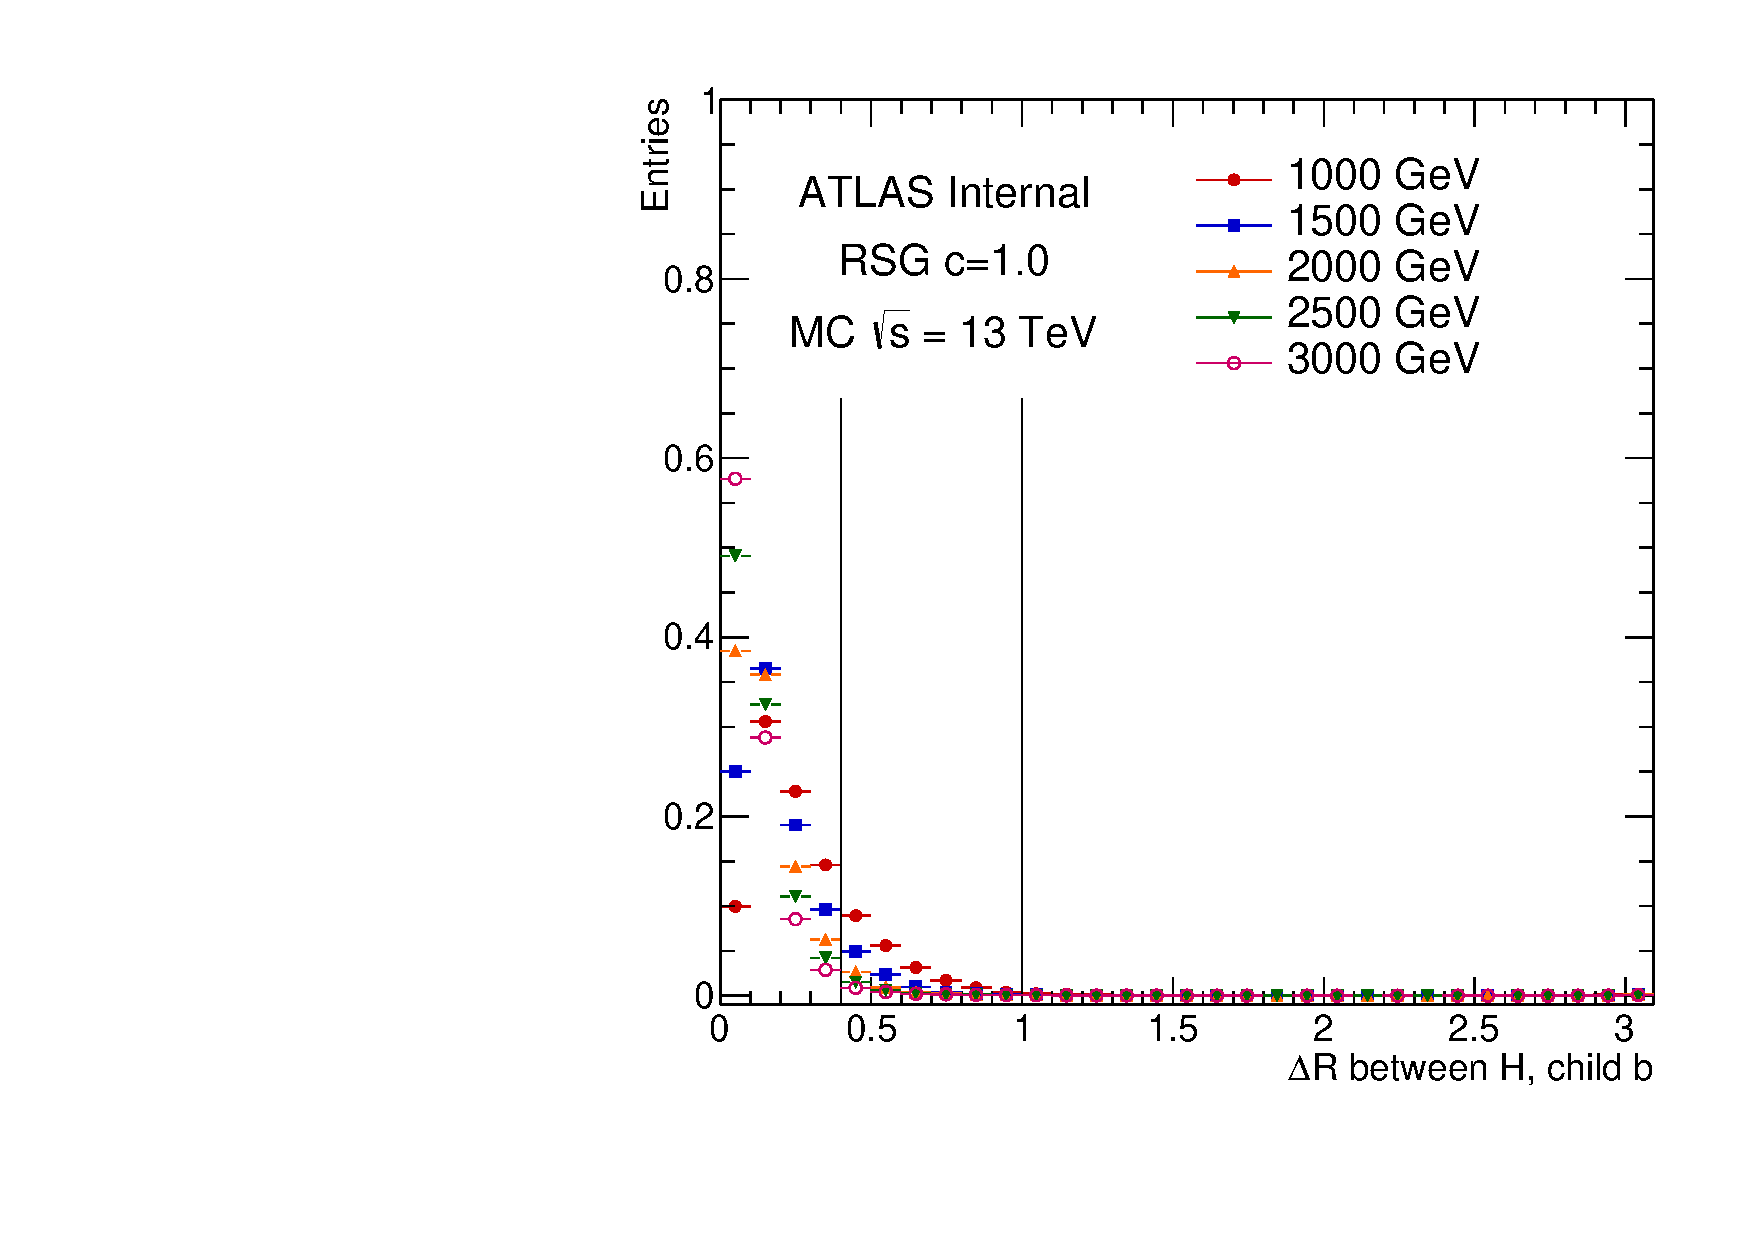
\includegraphics[width=0.45\textwidth,angle=-90]{figures/boosted/Truth/truth_hbdR.pdf}
  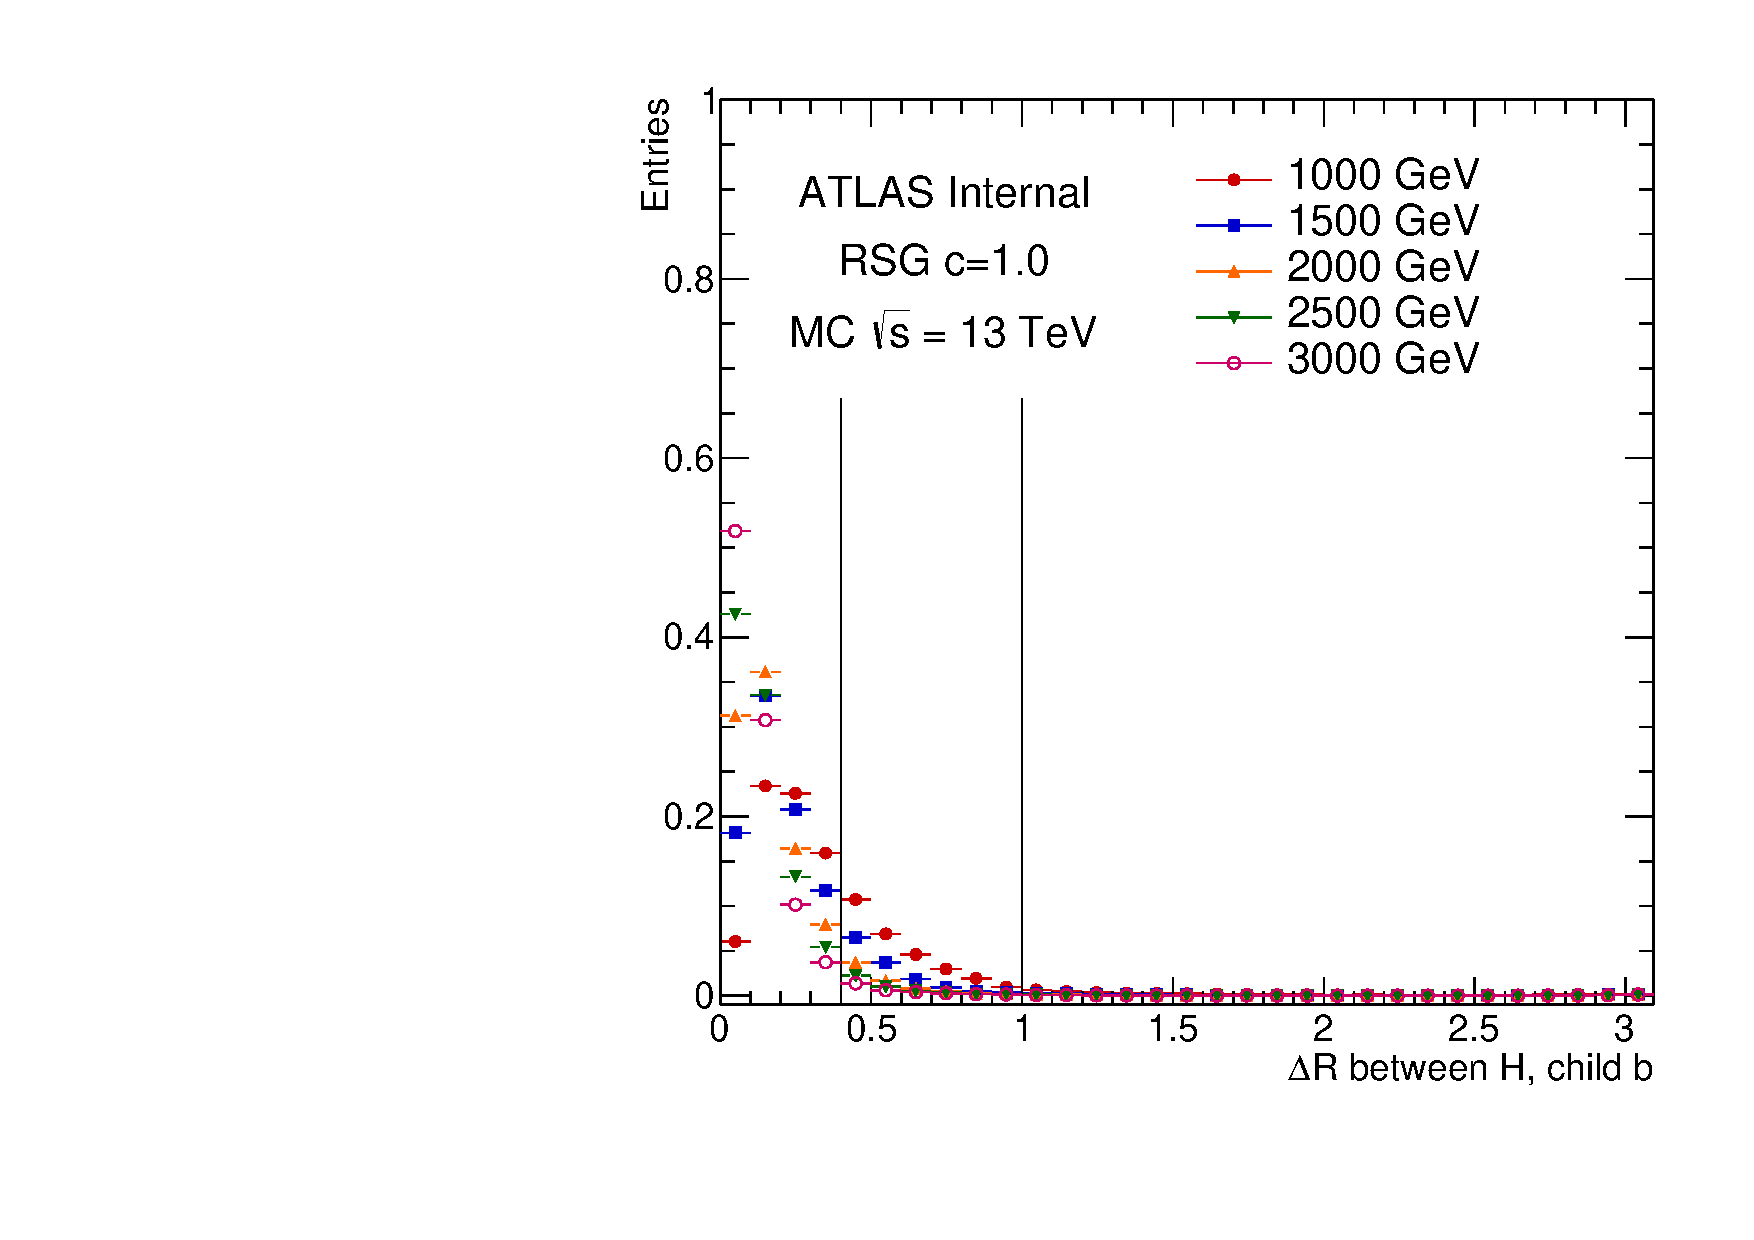
\includegraphics[width=0.45\textwidth,angle=-90]{figures/boosted/Truth/truth_hbdR2.pdf}
\caption{Normalized $\Delta R$ between the truth Higgs (leading on left, subleading on right) and the truth children $b$-quarks for \Grav~ MCs. Lines are drawn at $\Delta R = 0.4$ ($R$ of small-\R jets) and $\Delta R = 1.0$ ($R$ of large-\R jets). }
\label{fig:truth-HbdR}
\end{center}
\end{figure}

\paragraph{}
The track jets are required to have \pt $> 10$ \GeV, $|\eta| < 2.5$ and at least two tracks associated with it. 
A track jet is considered $b$-tagged if it has MV2c10 > $0.6455$, see Section~\ref{sec:btag_70wp} for details. 
Each large-\R jet is required to have at least one, not two, track jet Ghost associated with it.
This accounts for the $R=0.2$ track jets merging at really high boost, from signals above $2.5$ \TeV.
If there are more than one track jet contained in the large-\R jet, they are also sorted by \pt.
The highest \pt~ track jet is named as the leading track jet, and the second highest \pt~ one is named as the subleading track jet.
Only the two highest \pt~ track jet is considered in this thesis.
The one or two track jets $\Delta R$ match to the truth $b$ quarks $80\%$, as shown in Figure~\ref{fig:truth-bmatch}. 
In the Figure, red means the truth Higgs doesn't match the large-\R jet. Blue means both truth $b$ matches the two track jets. Orange means two truth $b$ matches one same track jet. Green indicates one $b$ quark has $\Delta R<0.2$ for both leading and subleading track jet, and the other $b$ is matched to one of the two track jets. Pink means one $b$ quark matches to one of the two track jets, the other $b$ doesn't match to the two leading track jets.

\begin{figure}[htbp!]
\begin{center}
  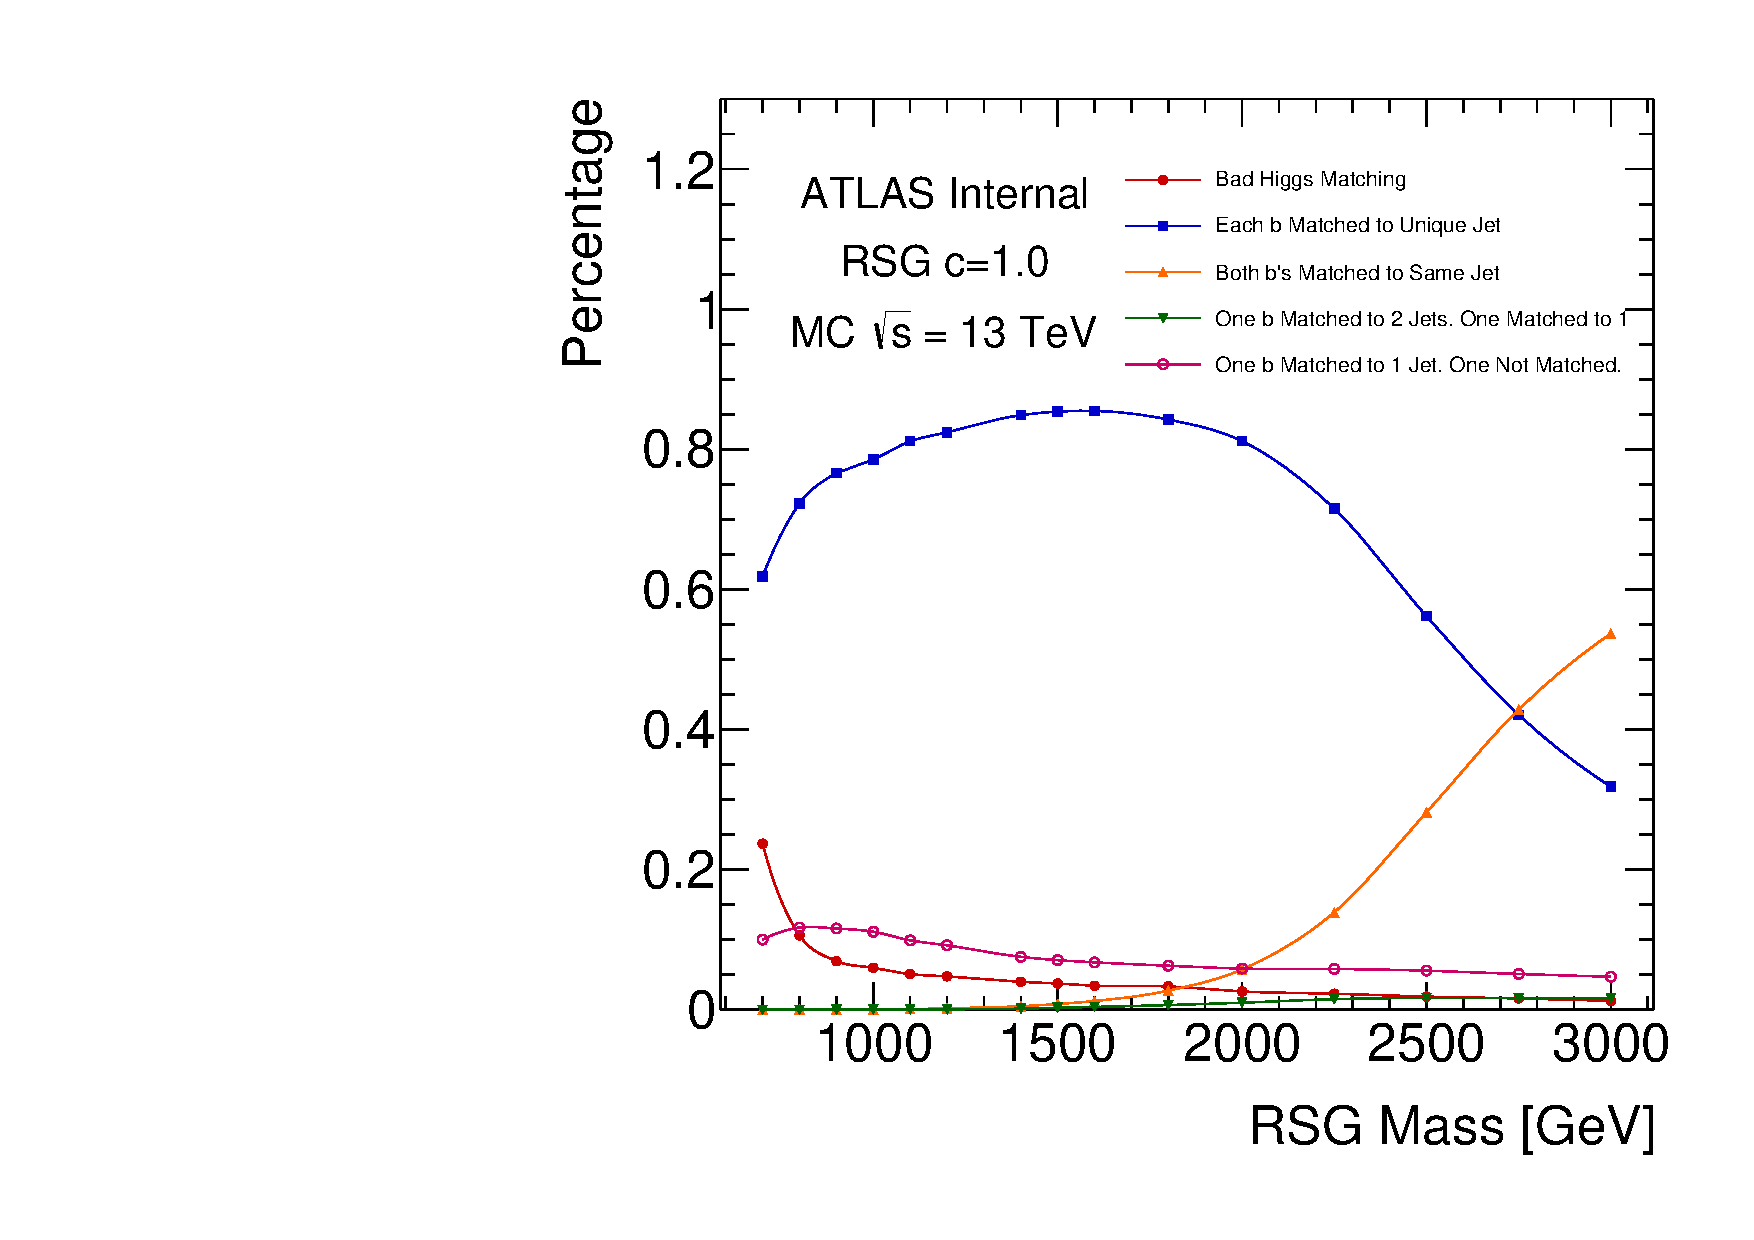
\includegraphics[width=0.45\textwidth,angle=-90]{figures/boosted/Truth/truth_b-matching.pdf}
  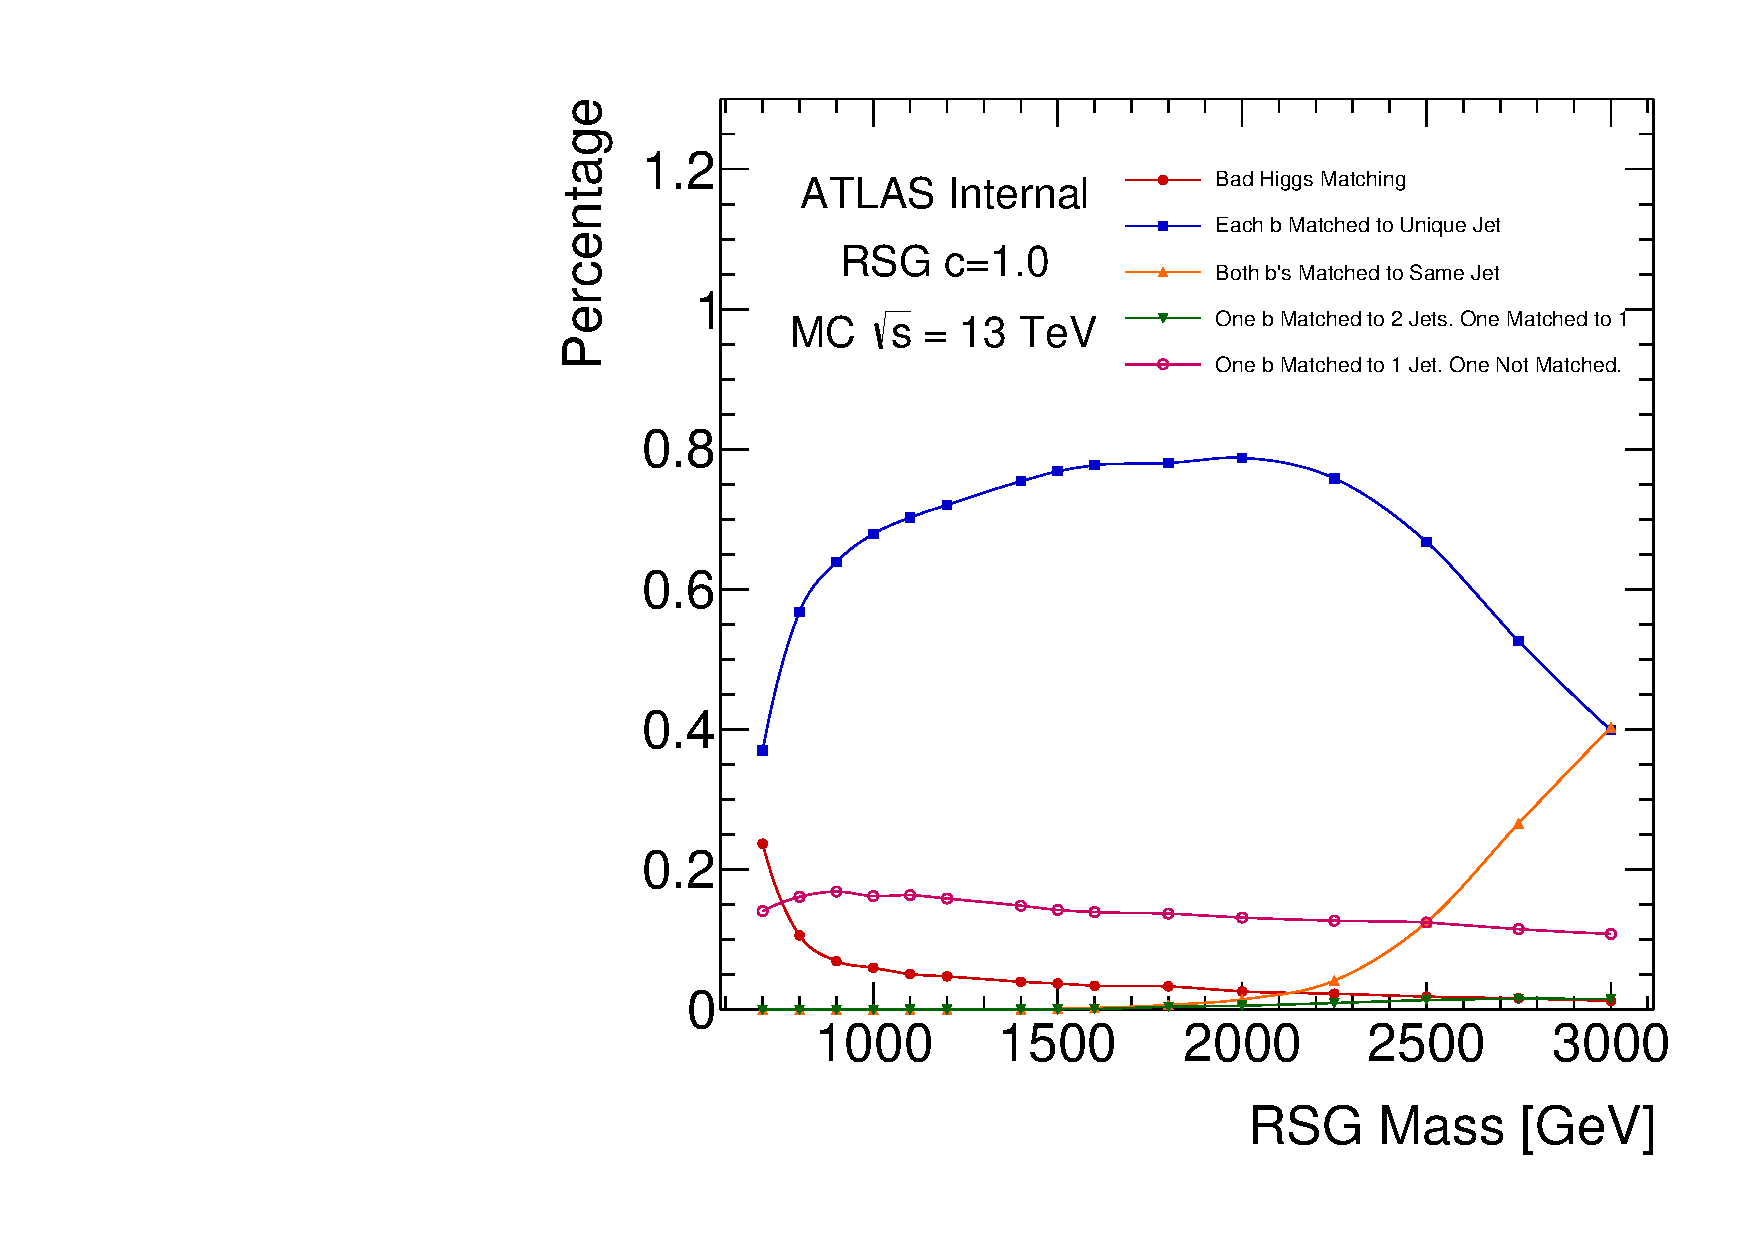
\includegraphics[width=0.45\textwidth,angle=-90]{figures/boosted/Truth/truth_b-matching-sublead.pdf}
\caption{Percentage of $\Delta R<0.2$ matching truth $b$'s to track jets (leading Higgs on the left, subleading Higgs on the right) for different \Grav~ mass. The cases listed in the legend are orthogonal to each other. The cases not listed on the legend (including when a truth $b$ is not contained in the large-\R jet) happen in total at most $1.6\%$ of the time for a given \Grav~ mass.}
\label{fig:truth-bmatch}
\end{center}
\end{figure}

\paragraph{}
A further muon correction accounts for energy loss due to leptonic $b$-hadron decays with a muon in the final state.
The muon-in-jet corrections are applied only after the fiducial large-\R jet requirements on \pt and $\eta$.
The muons are required have $\Delta R < 0.2$ with the $b$-tagged track jets within each large-\R jet. 
In case more than one muon is found within a track jet, only the muon with the smallest $\Delta R$ is considered. 
If two $b$-tagged track jets are found to have muons, both corrections are considered. 
The four-momenta of the matched muon is added to the large-\R jet four-momentum, with the muon calorimeter energy deposits subtracted. 
This correction is only applied to the calorimeter mass portion of the combined mass. 
The muon-in-jet correction improves the large-R jet mass resolution by approximately 5\%, and Figure~\ref{fig:boosted-muons-signal} shows the impact of this correction on the 1 \TeV~ \Grav.

\begin{figure*}
\begin{center}
  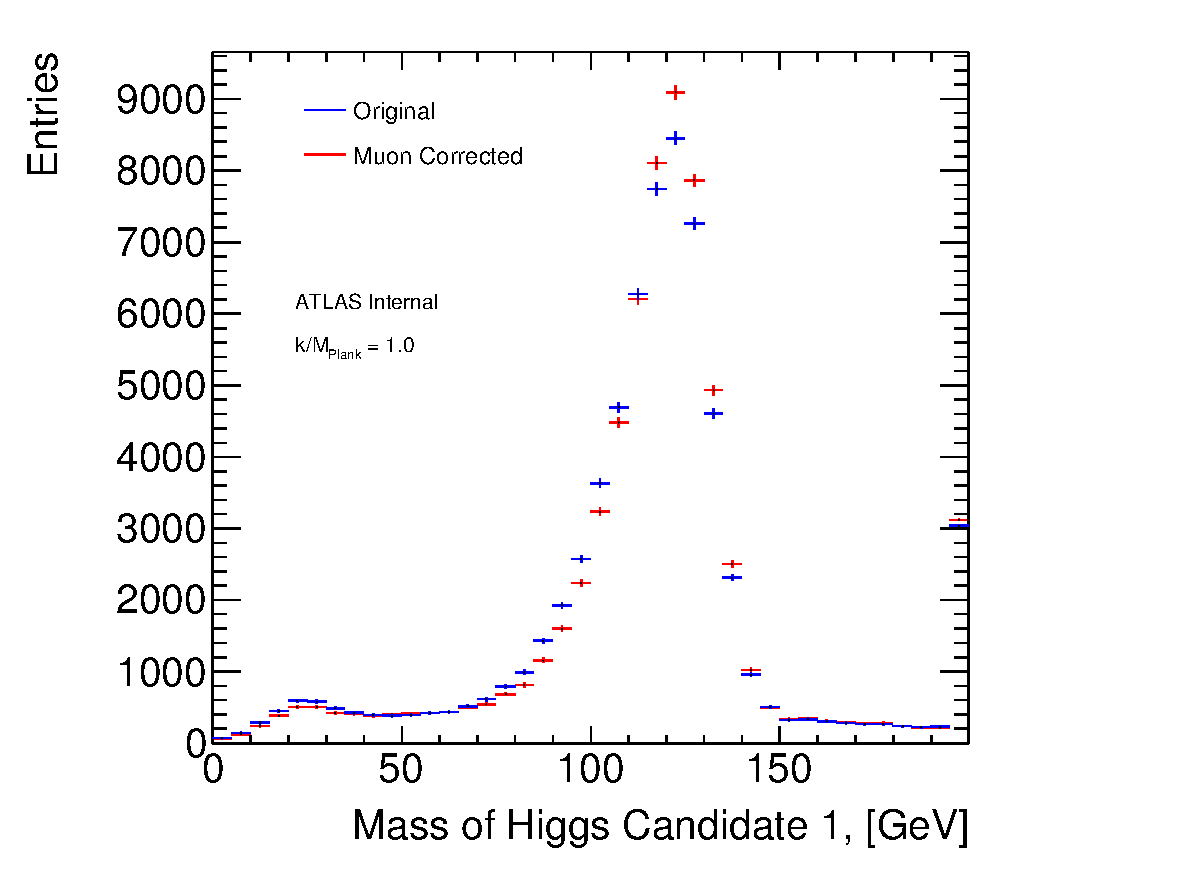
\includegraphics[width=0.48\textwidth]{figures/boosted/muons/h1_mass_dbl.pdf}
  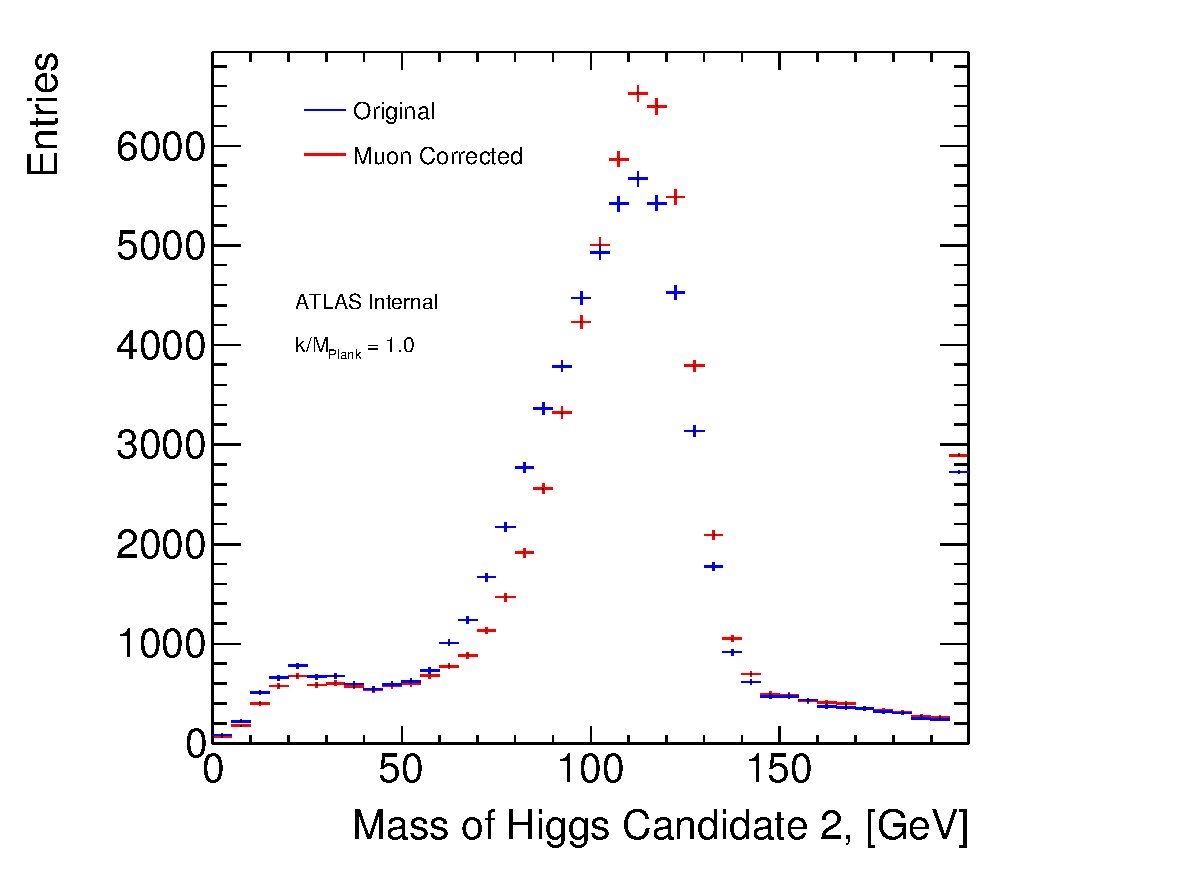
\includegraphics[width=0.48\textwidth]{figures/boosted/muons/h2_mass_dbl.pdf}
  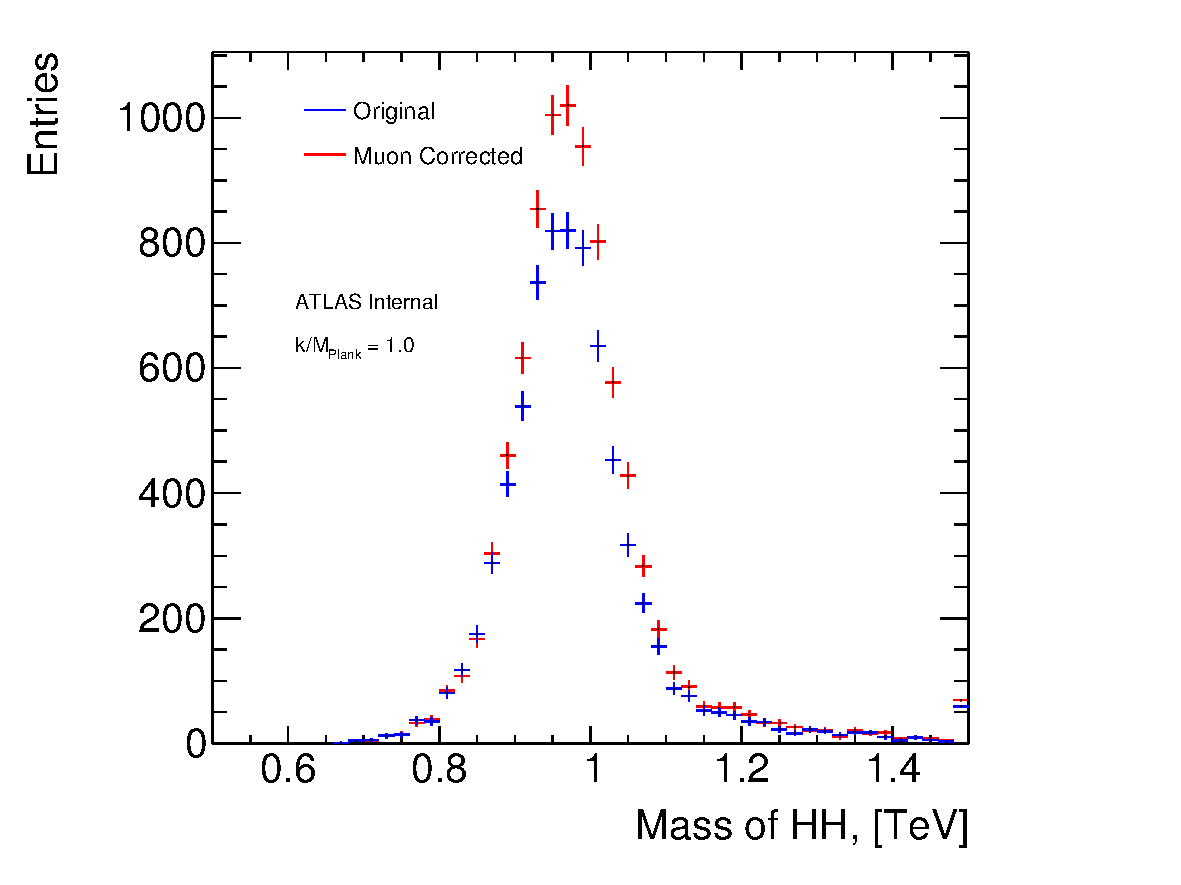
\includegraphics[width=0.48\textwidth]{figures/boosted/muons/hh_mass_dbl.pdf}
  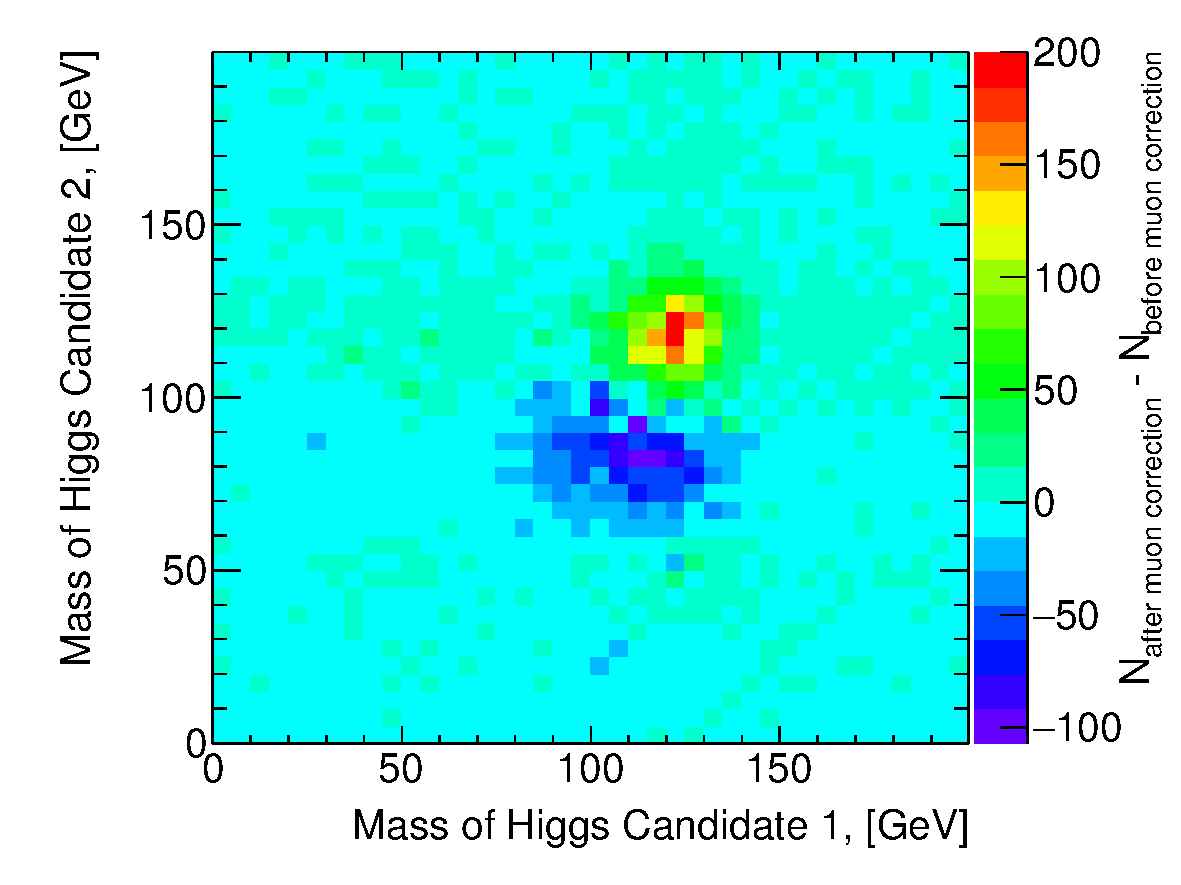
\includegraphics[width=0.48\textwidth]{figures/boosted/muons/h12_corr_mass.pdf}
  \caption{Kinematics of $1$ \TeV~ \Grav~ before and after muon-in-jet corrections. The reconstructed Higgs masses (top row, left for leading large-\R jet, right for subleading large-\R jet) are closer to $125$ \GeV after the correction, which improves the signal efficiency for the signal region selection by $\sim\!10\%$ (bottom row, left for $m_{JJ}$, right for event distribution differences on the leading-subleading large-\R jet mass plane.).}
  \label{fig:boosted-muons-signal}
\end{center}
\end{figure*}

\paragraph{}
Finally, the Higgs candidates (large-\R jets) are also required to have $|\Delta\eta| = |\eta_{\text{leadJ}} -\eta_{\text{sublJ}} |< 1.7$. 
This is because the spin 2 \Grav~ are produced mostly through s-channel, while the multijet events could also be produced through t-channels or u-channel. 
Figure ~\ref{fig:app-check-deta} shows the distribution for signal sample and data inclusive $b$-tag region $\Delta \eta_{JJ}$ distribution.
This cut is not entirely optimal for Scalar signals due to the different spin, yet it is fixed for both \Grav~ and Scalar selections.

\begin{figure*}
\begin{center}
  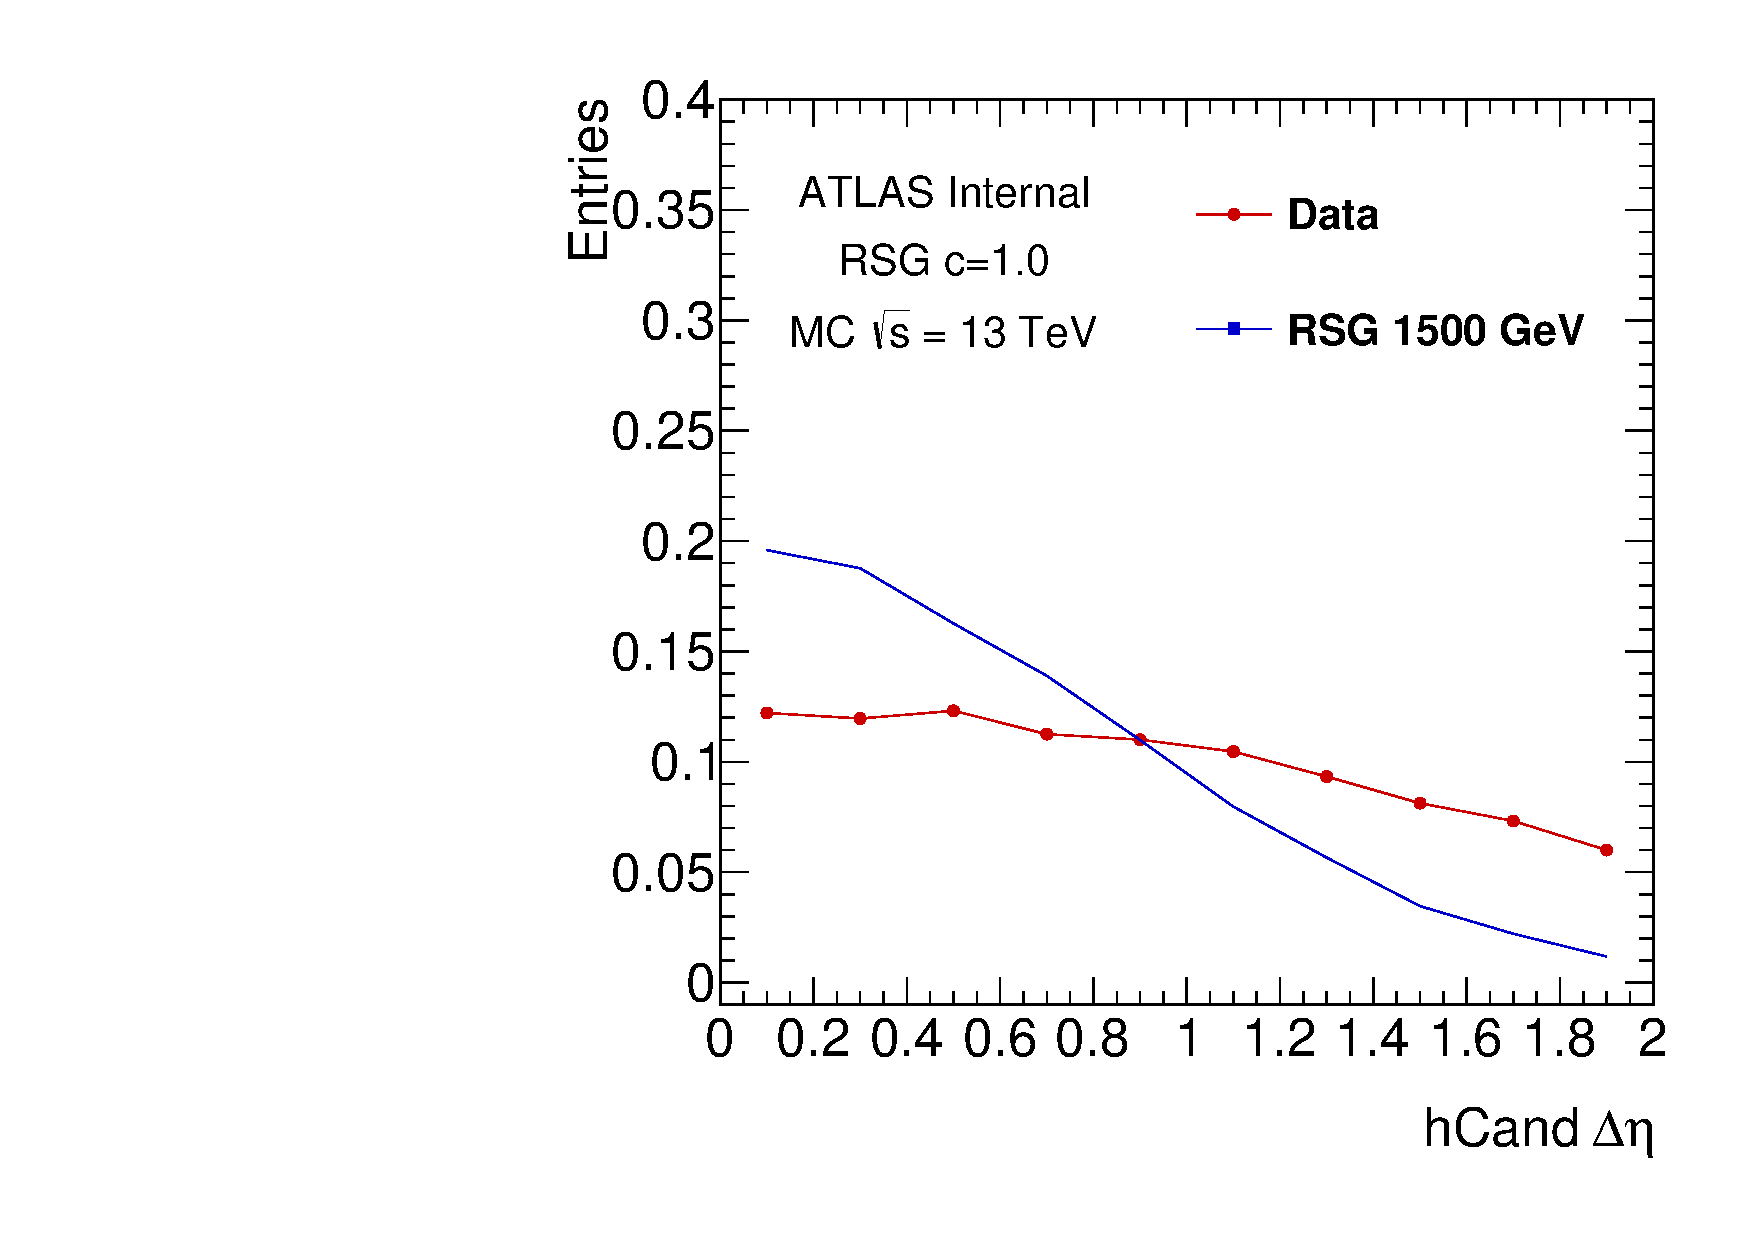
\includegraphics[width=0.45\textwidth,angle=-90]{figures/boosted/Other/AllTag_Signal_hCandDeta_F_c10-cb-no-deta-cut_truth_0.pdf}
  \caption{ After large-\R jet requirements, normalized $\Delta \eta_{JJ}$ distribution in $1.5$ \TeV \Grav~ and data, where the data consists of mostly multijet events (> 90$\%$). The background multijet event is flatter in $\Delta \eta_{JJ}$ distribution.}
\label{fig:app-check-deta}
\end{center}
\end{figure*}


%%%%%%%%%%%%%%%%%%%%%%%%%%%%%%%%%%%%%%%%%%%%%%%%%%%%%%%%%%%%%%%%%%%%%%%%%%%%%%%%%%%%%%%%%%
\section{Resolved Veto}
\label{sec:resollvedveto}

\paragraph{}
Sometimes one event can be reconstructed in both the resolved method as four small-\R jets and the boosted method as two large-\R jets with track jets. Figure~\ref{fig:obj_evt_display} shows an example event display of collision data recorded in 2015.

\begin{figure}[h!]
\centering
\captionsetup{justification=centering}
    \begin{subfigure}[b]{0.45\textwidth}
        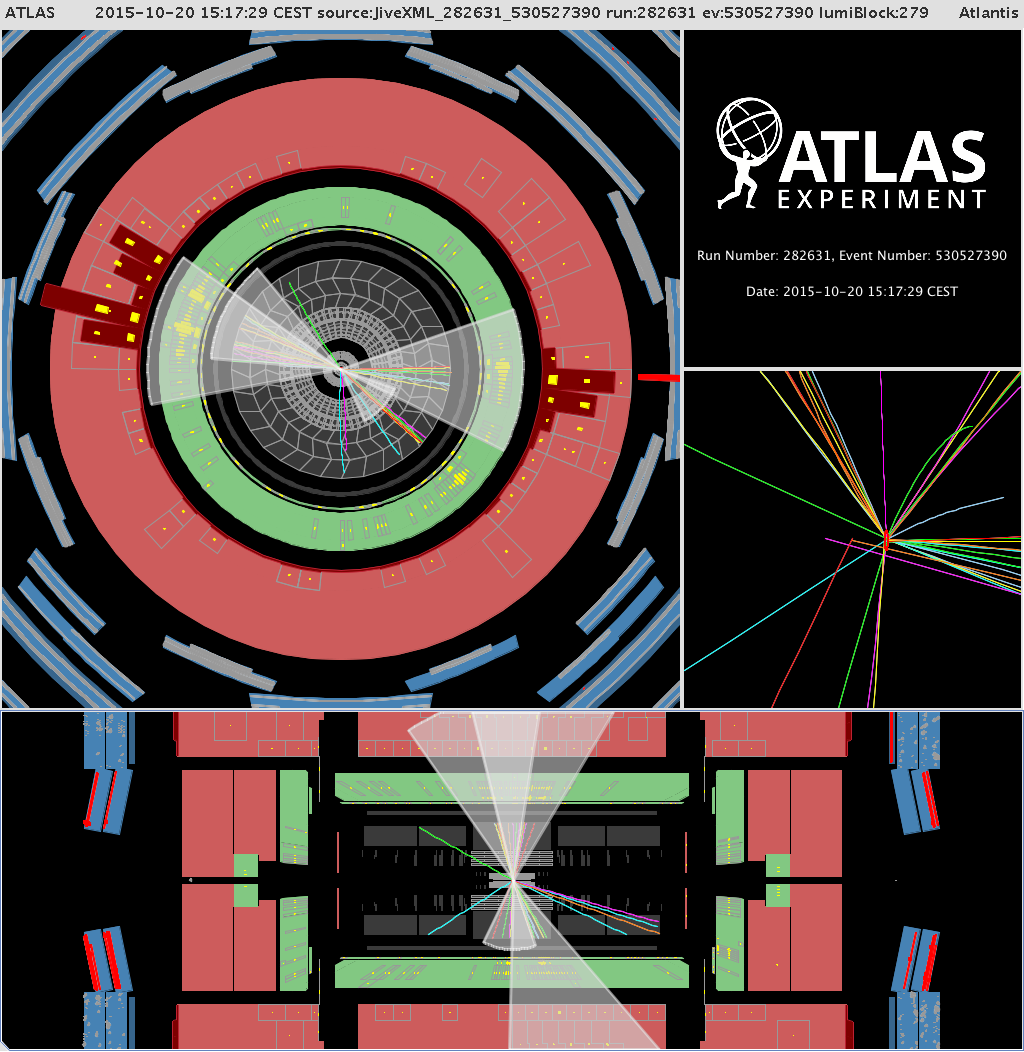
\includegraphics[width=\textwidth]{figures/object/JiveXML_282631_530527390-YX-RZ-YZ-EventInfo-2016-02-29-15-48-39}
        \caption{Resolved reconstruction.}
        \label{fig:obj_evt_display_resolved}
    \end{subfigure}
    \quad
    \begin{subfigure}[b]{0.45\textwidth}
        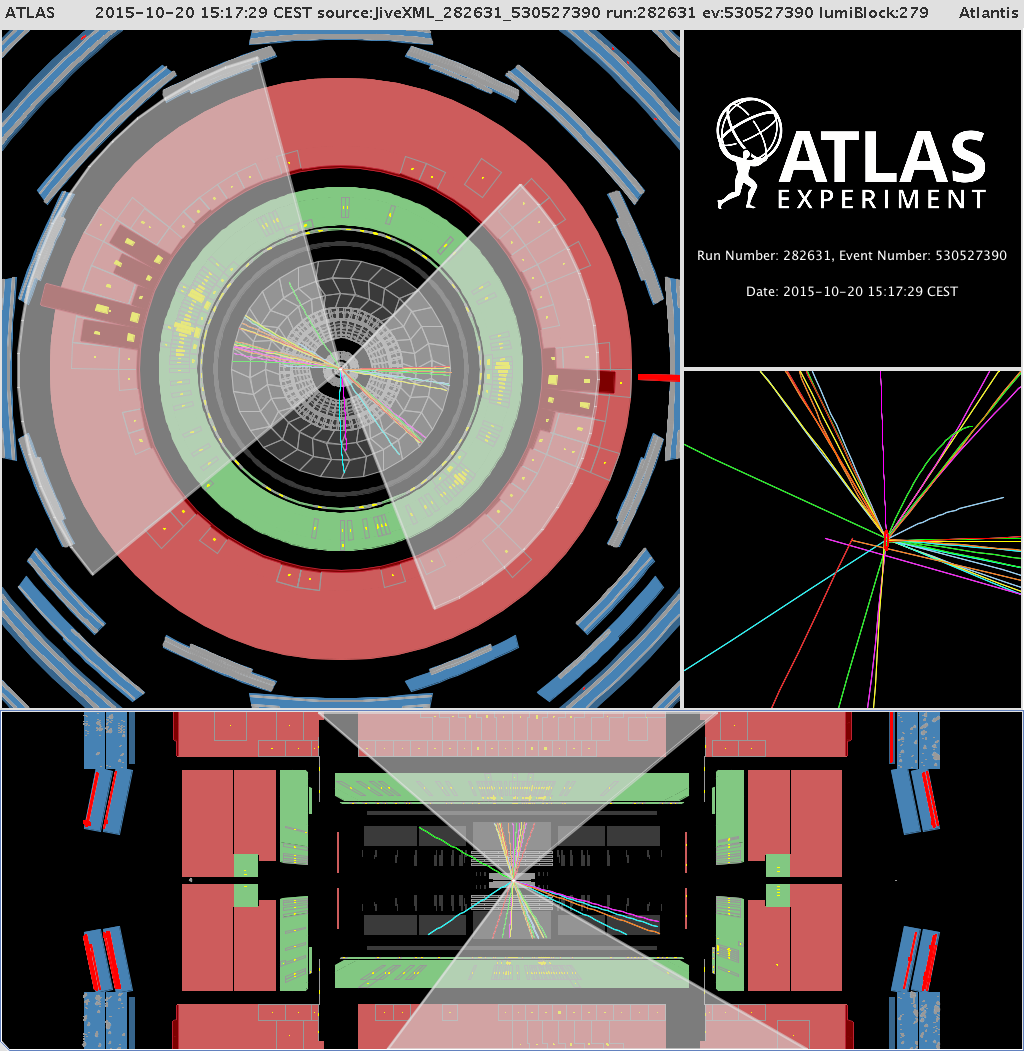
\includegraphics[width=\textwidth]{figures/object/JiveXML_282631_530527390-YX-RZ-YZ-EventInfo-2016-02-29-15-48-08}
        \caption{Boosted reconstruction.}
        \label{fig:obj_evt_display_boosted}
    \end{subfigure}
\caption{Event display of the same event using ~\ref{fig:obj_evt_display_resolved} resolved and ~\ref{fig:obj_evt_display_boosted} boosted topologies. The resolved reconstruction gives a $m_{4J}$ of $873$ \GeV~, and the boosted reconstruction gives $m_{2J}$ of $852$ \GeV. }
\label{fig:obj_evt_display}
\end{figure}

\paragraph{}
In order to avoid events being reconstructed by both the resolved and the boosted analysis, events that pass the resolved signal region selections are vetoed in the boosted analysis.
This is a political decision, and the effect of vetoing boosted event selection in the resolved analysis is never tested.
The gain is a full statistical combination of the resolved and boosted result.
For boosted analysis,  it hurts the sensitivity up to $1.5$ \TeV for resonance signals.
Hence it is necessary to introduce the resolved selection.

\paragraph{}
For resolved analysis, four small-\R jets with the highest $b$-tagging score are paired to construct two Higgs boson candidates.  
Each jet must have \pt $> 40$ \GeV~, $|\eta| < 2.5$, MV2c10 $> 0.8244$ (small-\R jet $70\%$ $b$-tagging working point). 
Pairings of jets into Higgs boson candidates are only accepted if they satisfy the following requirements, where \mfourj is expressed in \GeV:\\
if \mfourj  < 1250\,\GeV:
\begin{equation}
\frac{360\,\GeV}{\mfourj} - 0.5 < \DR_{jj}^{lead} < \frac{653\,\GeV}{\mfourj} + 0.475;\quad
\frac{235\,\GeV}{\mfourj} < \DR_{jj}^{subl}  < \frac{875\,\GeV}{\mfourj} + 0.35
\end{equation}
\quad if \mfourj  > 1250\,\GeV:
\begin{equation}
0< \DR_{jj}^{lead} < 1;\quad 0 < \DR_{jj}^{subl} < 1
\end{equation}
In these expressions, $\DR_{jj, \mathrm{lead}}$ is the angular distance between jets in the leading Higgs boson candidate and $\DR_{jj, \mathrm{subl}}$ for the sub-leading candidate. 
The leading Higgs boson candidate is defined to be the candidate with the highest scalar sum of jet \pt. 
This requirement efficiently rejects jet-pairings where one of the $b$-tagged jets is not consistent with that originating from a Higgs boson decay. 
The specific cut values in this and the following requirements were chosen to maximize the sensitivity to the signal.

\paragraph{}
Also, mass-dependent requirements are made on the leading Higgs boson candidate \pt, and the sub-leading Higgs boson \pt,:
\begin{equation}
p_T^{lead} > 0.5\mfourj - 105\,\GeV, \quad
p_T^{subl} > 0.33\mfourj - 75\,\GeV
\end{equation}
where \mfourj is again expressed in \GeV.

\paragraph{}
A further (\mfourj-independent) requirement is placed on the pseudorapidity difference between the two Higgs boson candidates, $\dEta < 1.5$, which rejects multijet events.
\begin{equation}
\dEta < 1.1 \quad \mathrm{if}\ \mfourj < 850\,\GeV , \quad
\dEta < 2\times10^{-3} \mfourj - 0.6 \quad \mathrm{if}\ \mfourj > 850\,\GeV
\end{equation}

\paragraph{}
Events that have multiple Higgs boson candidates satisfying these requirements (which happens often when $\mfourj < 500\,\GeV$) necessitate an algorithm to choose the correct pairs. 
In the absence of energy loss through semi-leptonic decays, the optimal choice would be the combination most consistent with the decays of two particles of equal mass.
To account for energy loss, the requirement of equal masses is modified. 
The distance, \Dhh, of the pairing's leading and subleading Higgs boson candidate masses, $\left(\leadm, \sublm\right)$ from the line connecting $\left(0\,\GeV, 0\,\GeV\right)$ and $\left(120\,\GeV, 110\,\GeV\right)$ is computed, and the pairing with the smallest value of \Dhh~ is chosen.
The values of 120\,\GeV\, and 110\,\GeV\, are chosen because they correspond to the median values of the narrowest intervals that contain 90\% of the signal in simulations.%the centre of the signal region in \leadm and \sublm respectively,
\Dhh~ can be expressed as follows:
\begin{equation}
D_{hh} = \frac{\left|\leadm - \frac{120}{110}\sublm\right|}{\sqrt{1+\left(\frac{110}{120}\right)^{2}}}.
\end{equation}

\paragraph{}
A requirement on the Higgs boson candidates' masses is used to define the resolved signal region:
\begin{equation}
X_{hh-resolved} = \sqrt{\left(\frac{\mlead - 120\,\GeV}{0.1\mlead}\right)^2 + \left(\frac{\msubl - 110\,\GeV}{0.1\msubl}\right)^2} < 1.6,
\label{eqn:resolvedXhh}
\end{equation}
where the 0.1\mtwoj terms represent the widths of the leading and sub-leading Higgs boson candidate mass distributions, derived from simulation. The signal region is shown as the inner region of Figure~\ref{fig:resolvedRegions}. In summary, for any event can make a Higgs candidate through the Dhh minimization and passing through the resolved signal region $X_{hh-resolved}$ cut, it is rejected in the boosted selection.

%For more detail, please see the resolved signal region definition. 
%For the impact on the boosted analysis, see Appendix ~\ref{sec:app-optimization-resveto}.

%%%%%%%%%%%%%%%%%%%%%%%%%%%%%%%%%%%%%%%%%%%%%%%%%%%%%%%%%%%%%%%%%%%%%%%%%%%%%%%%%%%%%%%%%%

\section{2D Higgs Mass Cut}

\begin{figure*}[htbp!]
\begin{center}
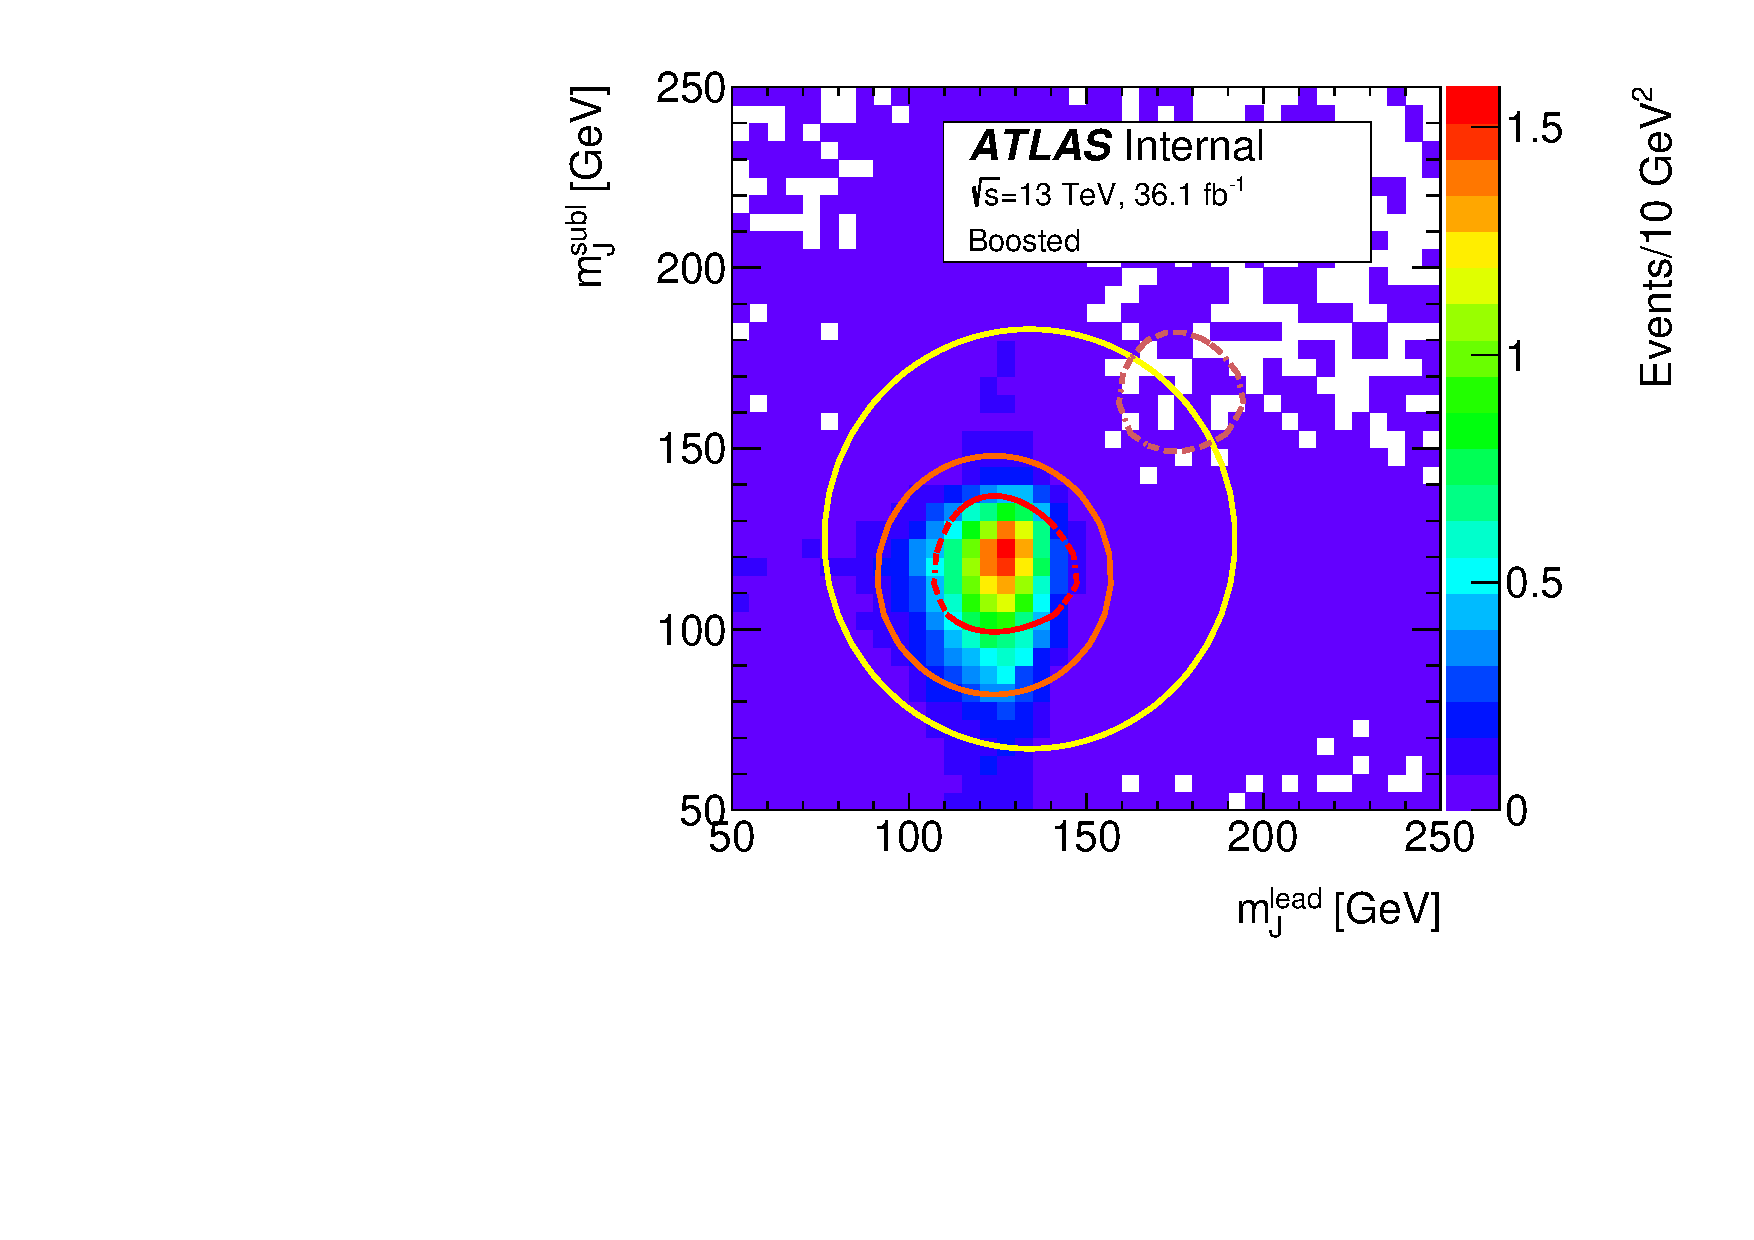
\includegraphics[width=0.35\textwidth,angle=-90]{figures/boosted/Truth/Sig_1200_AllTag_Incl_mH0H1.pdf}
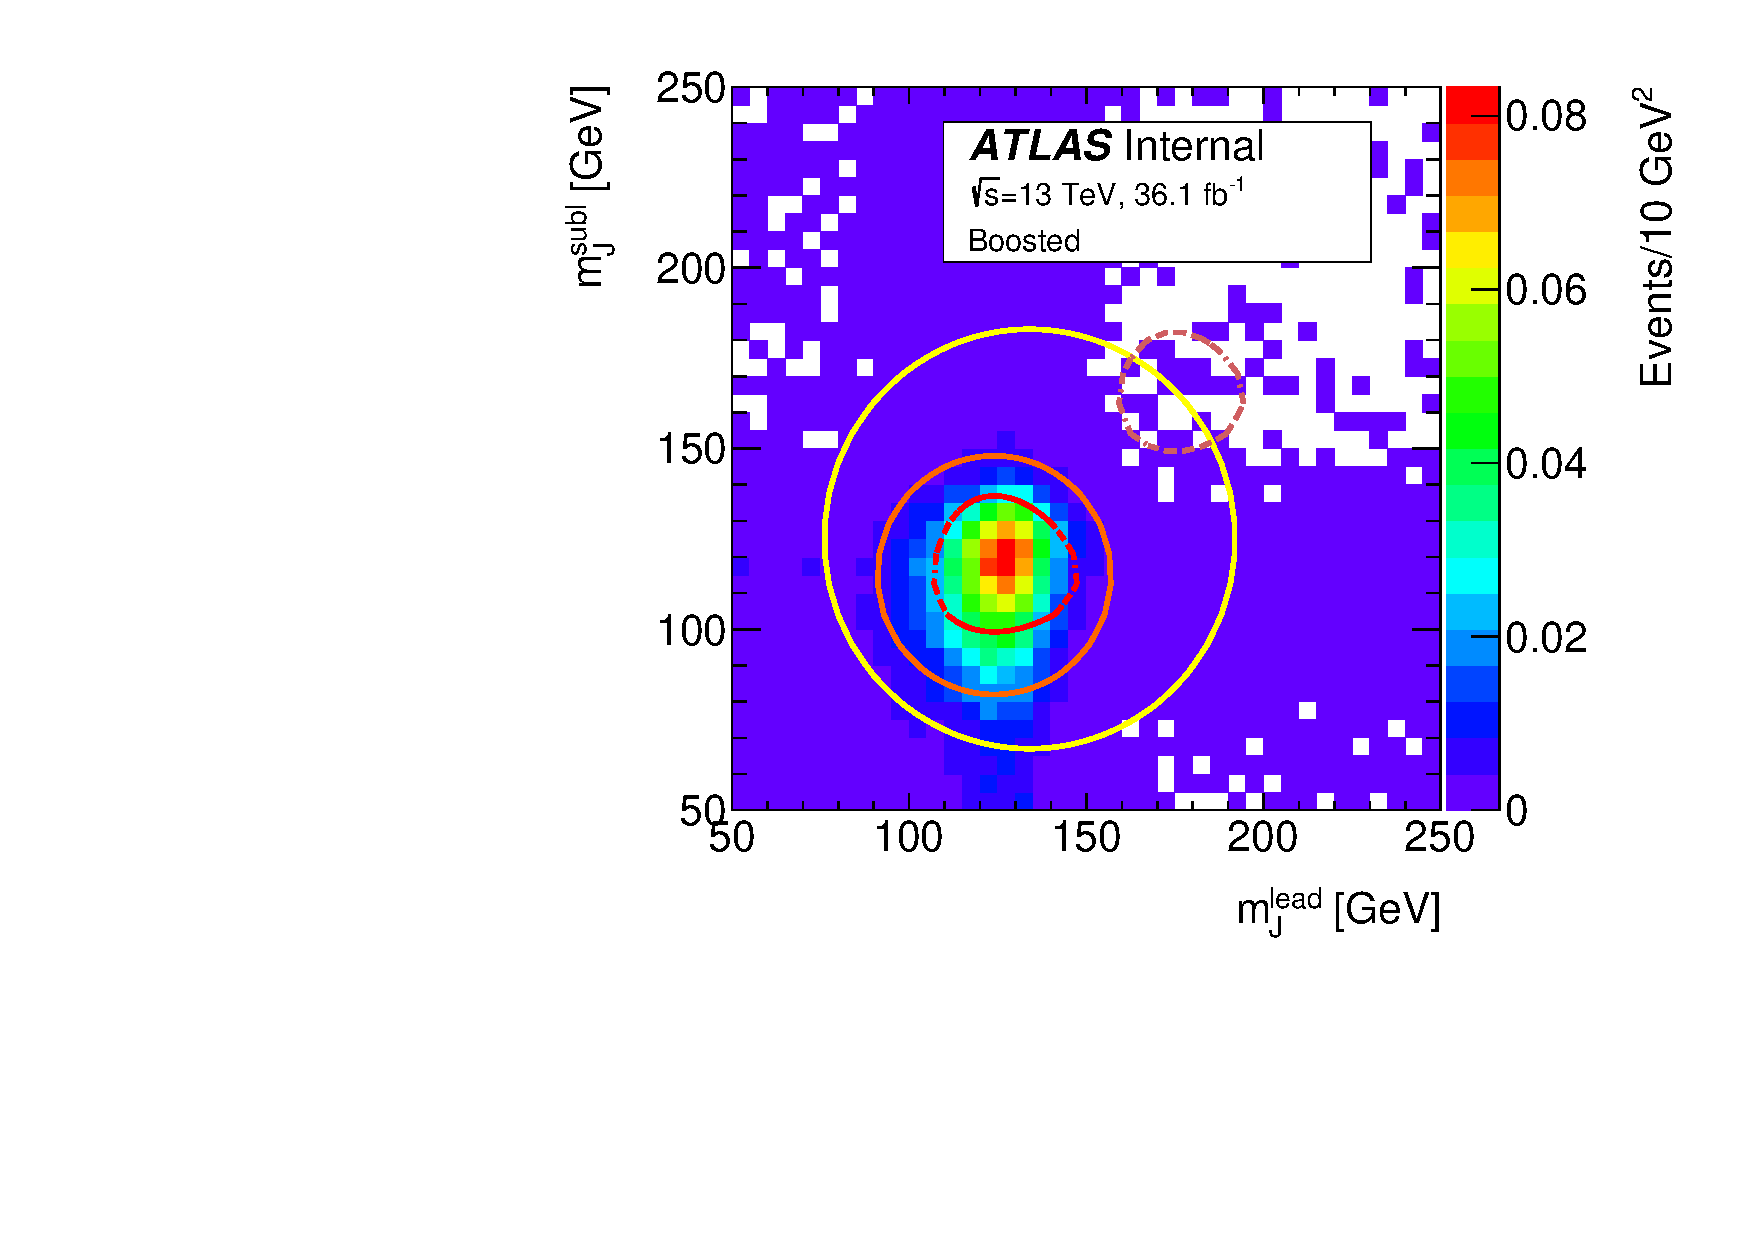
\includegraphics[width=0.35\textwidth,angle=-90]{figures/boosted/Truth/Sig_2000_AllTag_Incl_mH0H1.pdf}
\caption{For RSG $c=1.0$ samples, number of events as a function of leading Higgs candidate mass and subleading Higgs candidate mass, for $1.2$ \TeV~(left) signal and $2$ \TeV~(right) signal samples. The red dotted line in the center correspond to the signal region, passing $X_{hh} < 1.6$.}
\label{fig:evt-signal-mhh}
\end{center}
\end{figure*}

\paragraph{}
To separate di-Higgs decays from background productions like QCD multi-jets and top, requirements on the leading and subleading large-\R jet masses are imposed.
The signal region is defined using the expression~\ref{eq:boosted_XhhDef}:
\begin{equation}
\label{eq:boosted_XhhDef}
X_{hh} = \sqrt{\left(\frac{m^{\rm lead}_{\rm J} - \text{124 GeV}}{0.1 \left(m^{\rm lead}_{\rm J}\right)}\right)^2 + \left(\frac{m^{\rm subl}_{\rm J}- \text{115 GeV}}{0.1 \left(m^{\rm subl}_{\rm J}\right)}\right)^2}
\end{equation}

\paragraph{}
The denominator of each term in \Xhh~ can be interpreted as a resolution on the reconstructed mass of $10\%$ for the leading and subleading jets, hence \Xhh~ can be interpreted as a $\chi^2$ compatibility with the di-Higgs hypothesis.
The subleading jet mass value of $115$ \GeV~ is chosen after investigating the signal jet masses in MC. 
The subleading large-\R jet typically has a reconstructed mass which is biased downward. 
This is partly due to the ordering of the large-\R jets in \pt, which makes the subleading jet towards lower energy. 
The energy losses from neutrinos in leptonic $b$ decays, cracks in the calorimeter, and other effects also contributes. 
The signal region requires $X_{hh} < 1.6$. 
This cut gives nearly optimal performance. 
A more optimal signal region definition, using asymmetric signal jet mass resolution and a momentum dependent cut accounting for the higher mass resolution of lager \pt~ jets, can improve the overall sensitivity by $2-8\%$.
Since the gain in sensitivity is small, the signal region is kept to be consistent with the $X_{hh-resolved}$. Figure ~\ref{fig:evt-signal-mhh} shows the \Grav~ MC \mlead-\msubl 2D distribution.

%The denominator of each term in the definition can be interpreted as a resolution on the reconstructed mass of $8.5\%$ for the leading jet and $12\%$ for the subleading jet, hence $X_{hh}$ can be interpreted as a $\chi^2$ compatibility with the $hh$ hypothesis. Similarly to the resolved analysis, these $\sigma \left(m_{\rm J}\right)$ are only a rough approximation to the true resolution, but the $X_{hh}$ requirement gives nearly optimal performance. 
%The last substraction for high $p_\text{T}$ cases is because of the higher mass resolution of high mass signal samples. This effectively increases the size of $X_{hh}$ to 1.8 for a 3 TeV signal.

\section{Number of $b$-tagging requirement}
\paragraph{}
Passing basic object selection and \Xhh~ cut, the signal region selection is defined by further requiring multiple $b$-tags which are consistent with the di-Higgs decay. 
The presence of two \hbb~ decays in the final state naturally suggests requiring 4 track jets passing $b$-tagging requirements, and this is defined as the  $4b$ selection.

\paragraph{}
The $4b$ requirement has an overall efficiency of roughly $\epsilon^4$, where $\epsilon$ is the $b$-tagging efficiency chosen to be $70\%$.
This means an overall $0.7^4 \sim 0.24$ probability, but having one actual $b$-jet failling while the other three pass has probability $3 \times 0.7^3 \times (1-0.7) \sim 0.31$.
Therefore, a $3b$ selection is also introduced to recover the signal efficiency. 
An event with $3b$-tags must have at least $3b$-tagged track jets, but can have any number of additional un-tagged track jets.
In $4b$ and $3b$, each Higgs candidate can have at most two $b$-tagged track jets, hence $\geq 3b$-tagged trackjets cannot be in the same large-\R jet.

\paragraph{}
At the highest resonance mass, the Lorentz boost of the Higgs boson can be large enough to collimate the daughter $b$-quarks below the distance scale resolvable by the track jets ($R=0.2$). A third signal region is denoted by two-tag-split or simply $2bs$.
It requires exactly one $b$-tagged track jet is found in each Higgs candidate, plus an arbitrary number of track jets that must fail the $b$-tag.

\paragraph{}
$4b$, $3b$, and $2bs$ regions are chosen as three signal regions, also refered to as $n$-$b$tag regions.
The other $b$-tagging situations, also refered to as lower-$b$tag regions, are also sorted and studied.
$2b$ region is defined as one large-\R jet has two $b$-tagged track jets, and the other large-\R jet has no $b$-tagged track jet. 
$1b$ region is defined as one large-\R jet has one and only one $b$-tagged track jets, and the other large-\R jet has no $b$-tagged track jet. 
$0b$ region is defined as both large-\R jets have no $b$-tagged track jet. 
They all have relatively small signal acceptance. 

\paragraph{}
The MC events passing all signal region selections are sorted into different $b$-tagging categories. This is shown in Figure~\ref{fig:boosted-nbjet-signal-efficiency}. 
For masses above 2.5 TeV, the $2bs$ region (where each large-\R jet has exactly one $b$-tagged track jet) significantly improves the acceptance.
\begin{figure*}
\begin{center}
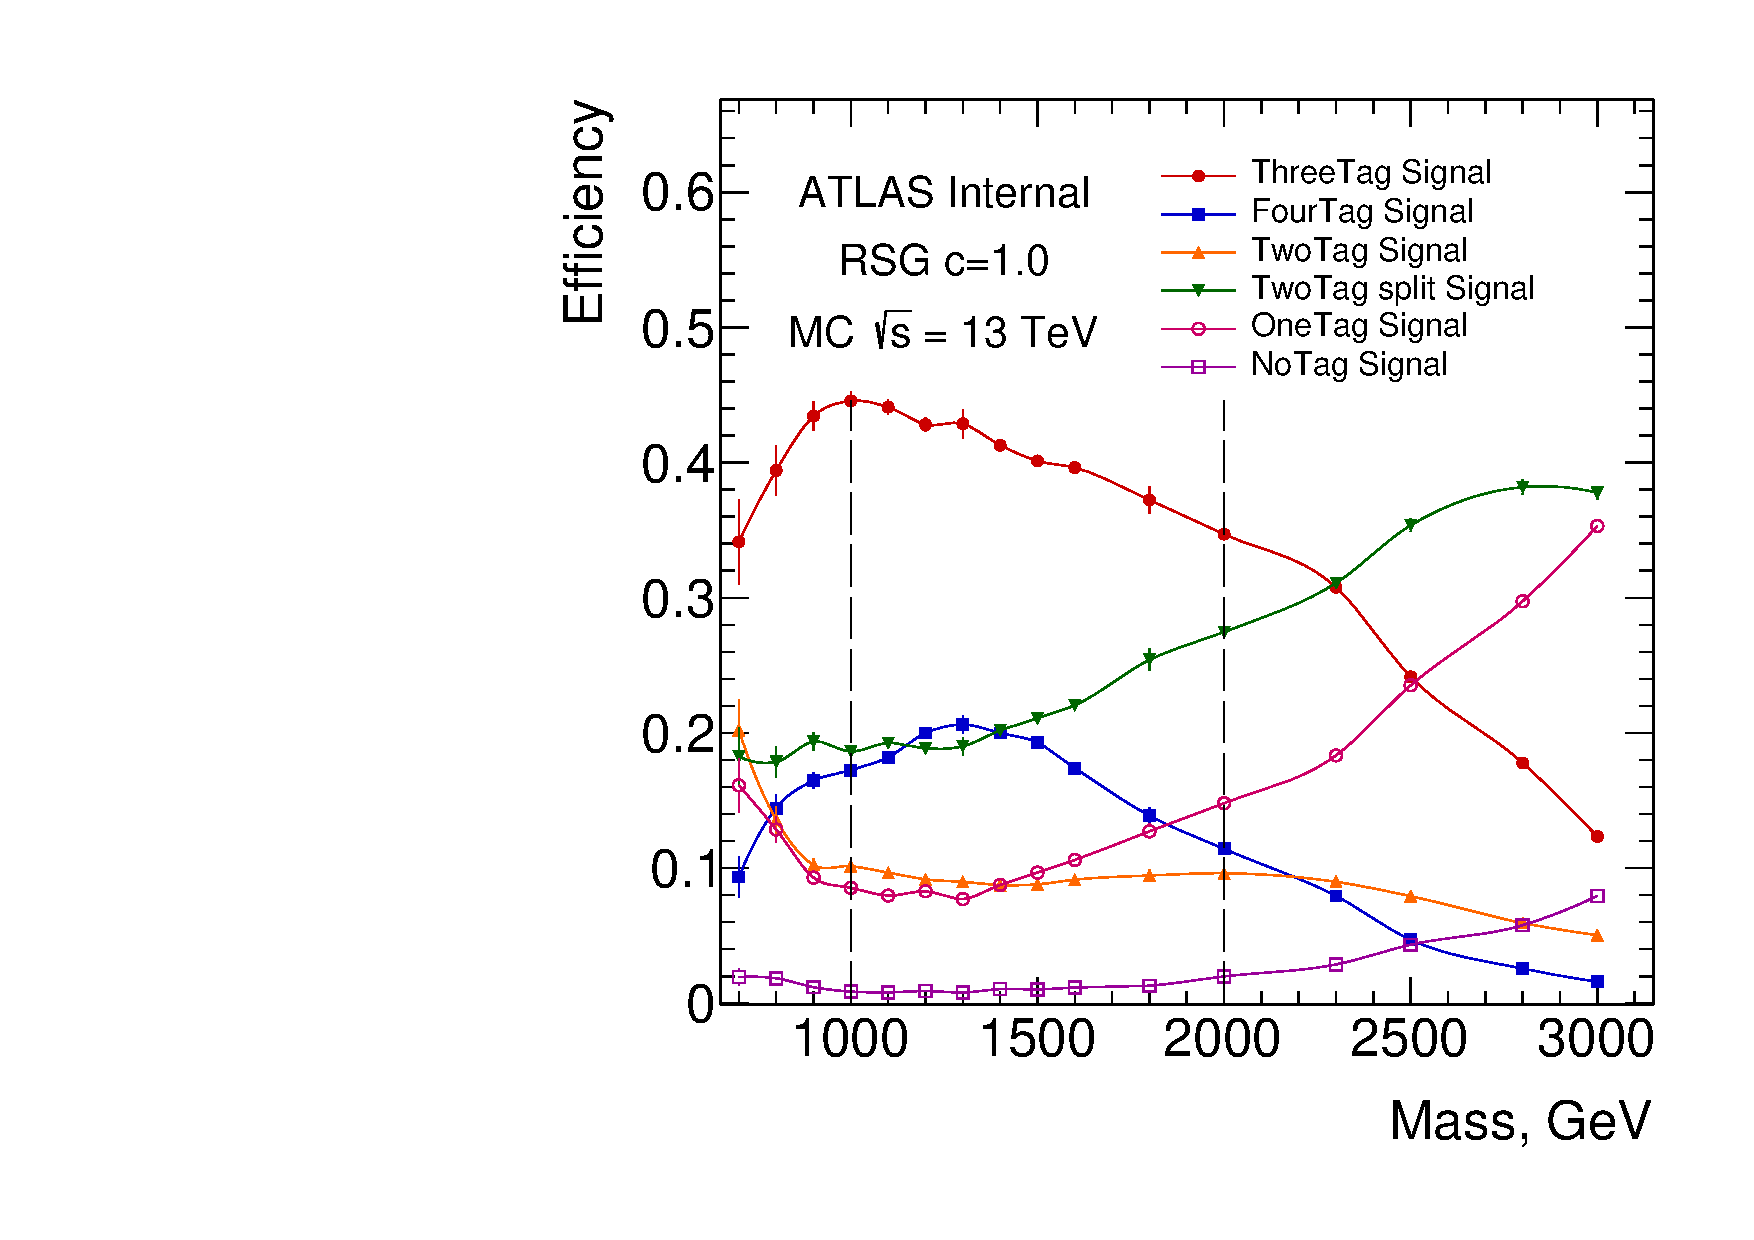
\includegraphics[width=0.48\textwidth,angle=-90]{figures/boosted/SigEff/region_lst_Moriond_Efficiency_AllTag_Signal.pdf}
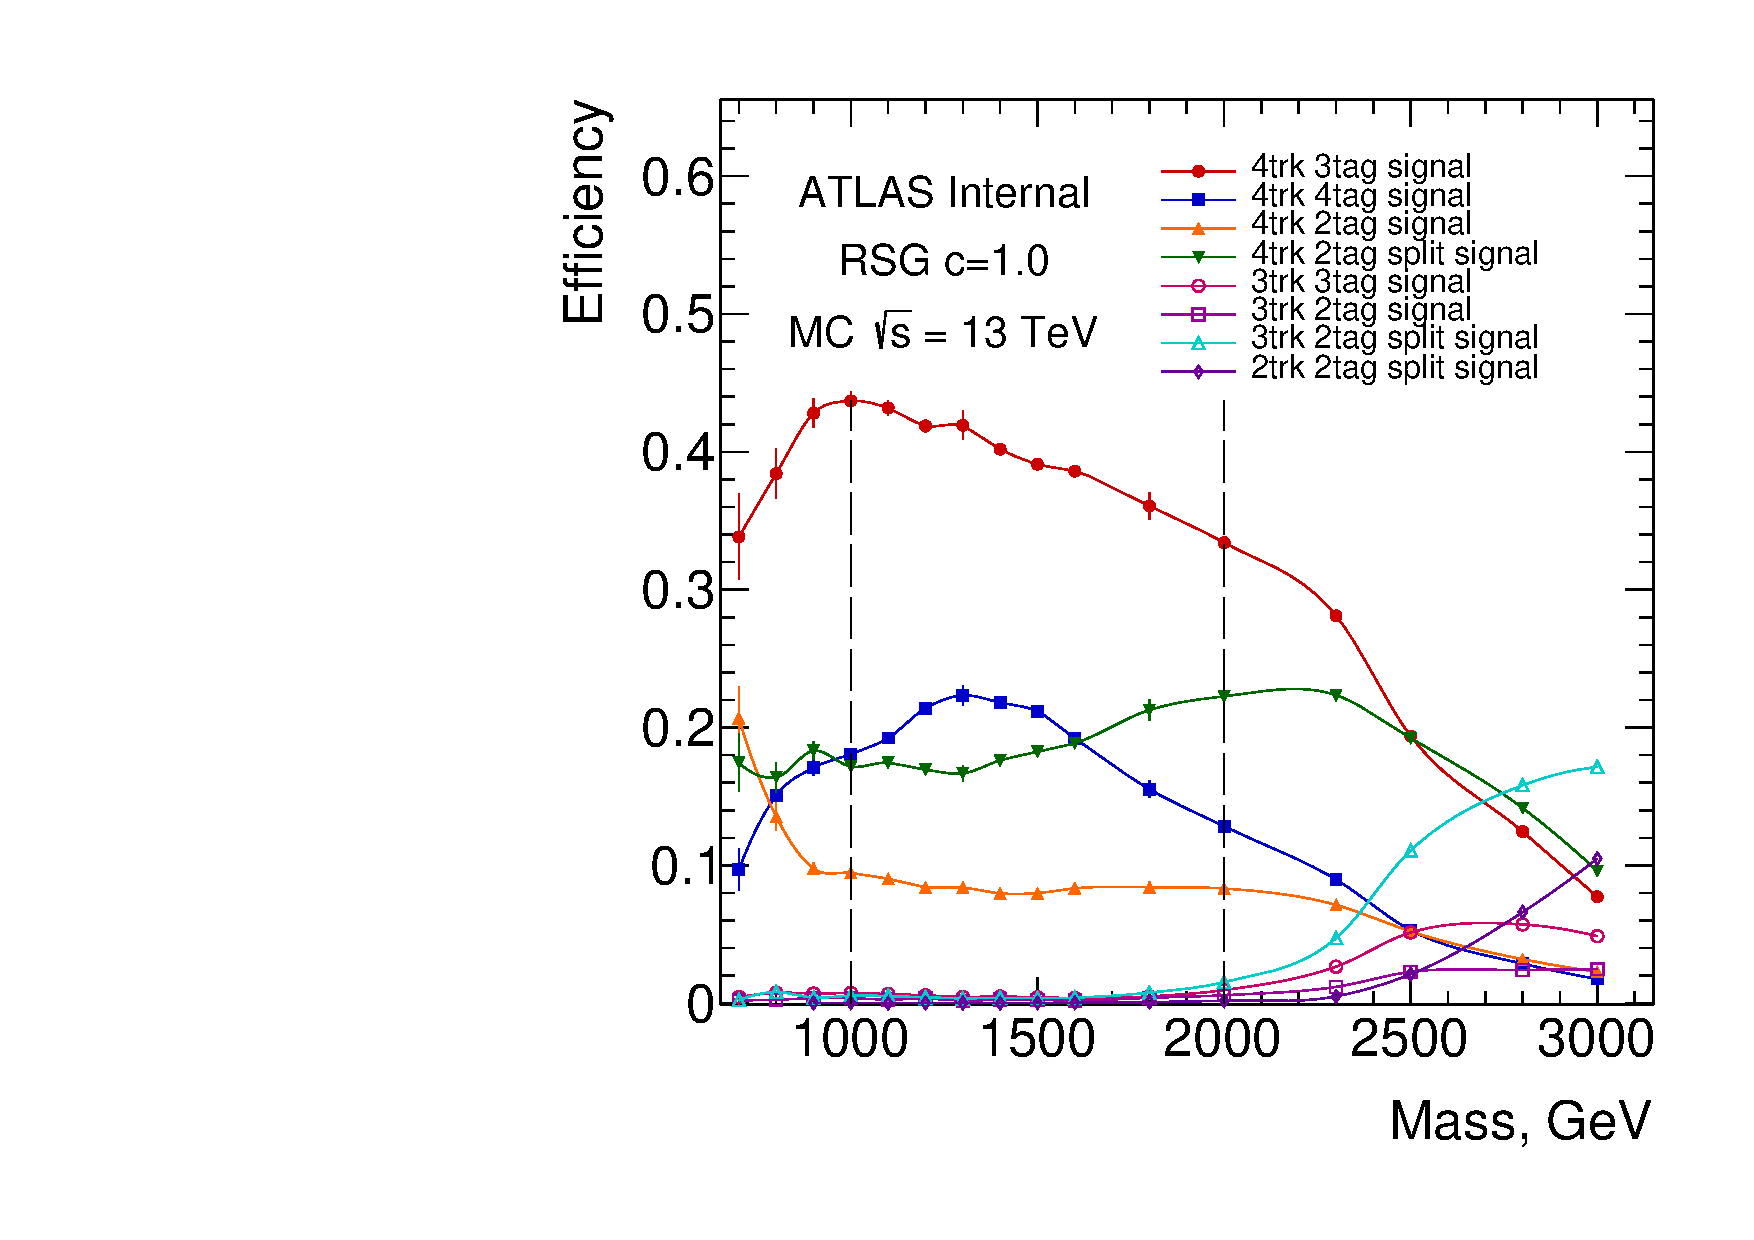
\includegraphics[width=0.48\textwidth,angle=-90]{figures/boosted/SigEff/detail_lst_Moriond_Efficiency_AllTag_Signal.pdf}
  \caption{Signal fraction in different $b$-tag categories (left) and detailed fraction in different number of track jet and $b$-tag categories (right) as a function of signal resonance mass hypothesis for selection cuts. The efficiencies are relative to the total number of events passing the 2D mass cut.}
  \label{fig:boosted-nbjet-signal-efficiency}
\end{center}
\end{figure*}



%%%%%%%%%%%%%%%%%%%%%%%%%%%%%%%%%%%%%%%%%%%%%%%%%%%%%%%%%%%%%%%%%%%%%%%%%%%%%%%%%%%%%%%%%%
\section{Signal efficiency and cutflow}
\paragraph{}
Acceptance means purely geometric fiducial volume of the detector. Efficiency refers to purely detector effectiveness in finding objects.
The signal efficiency as a function of \Grav~ resonance mass is shown in Figure~\ref{fig:boosted-selection-efficiency}, both for the absolute signal efficiency and for the efficiency relative to the previous cut in the selection.
Above a mass of $\sim\!1$ \TeV, the reconstruction of high momentum large-\R jets with small $\Delta\eta$ is efficient. 
Across the mass range considered, the signal jet masses requirement ($X_\text{hh}$) and $b$-tagging requirements are $\mathcal{O}(20\%)$ efficient relative to the previous cuts.

\begin{figure*}
\begin{center}
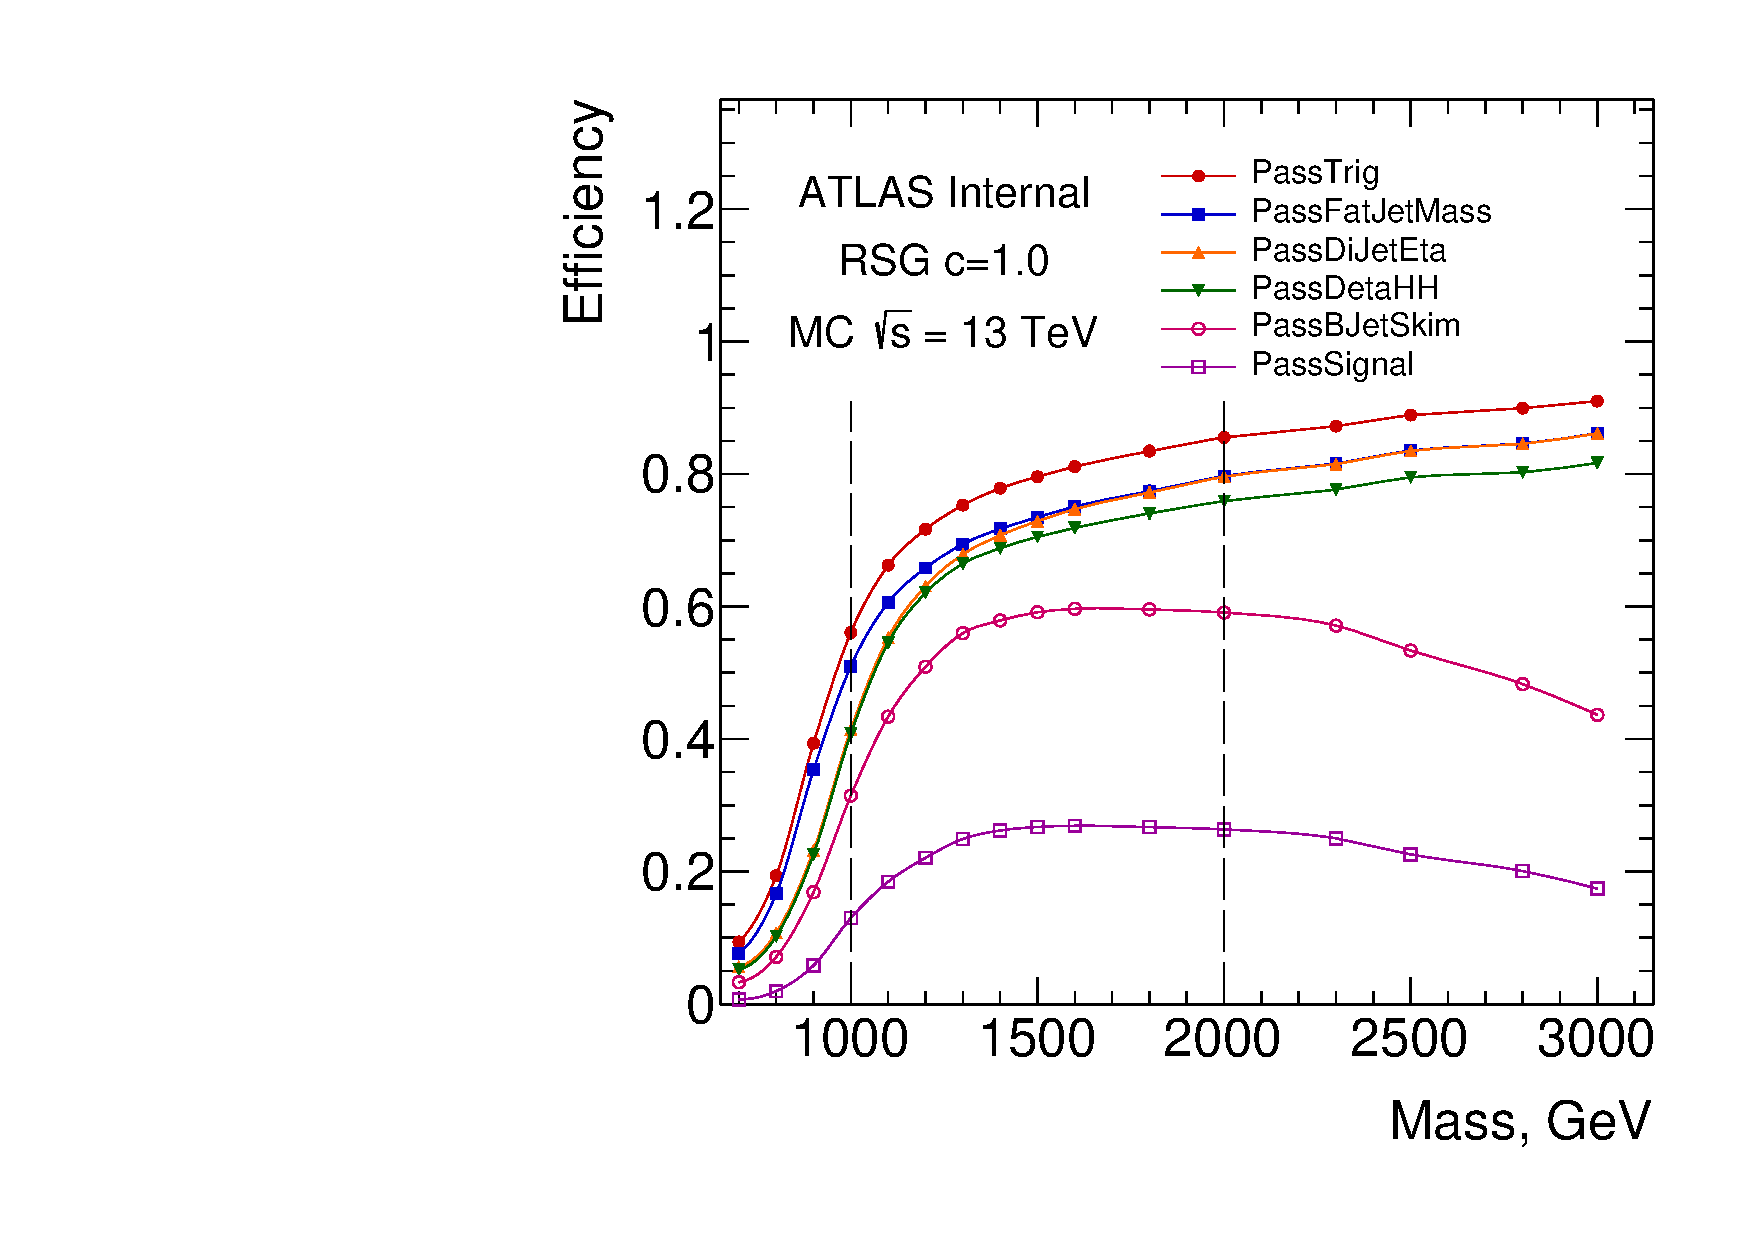
\includegraphics[width=0.48\textwidth,angle=-90]{figures/boosted/SigEff/evtsel_Moriond_Efficiency_PreSel.pdf}
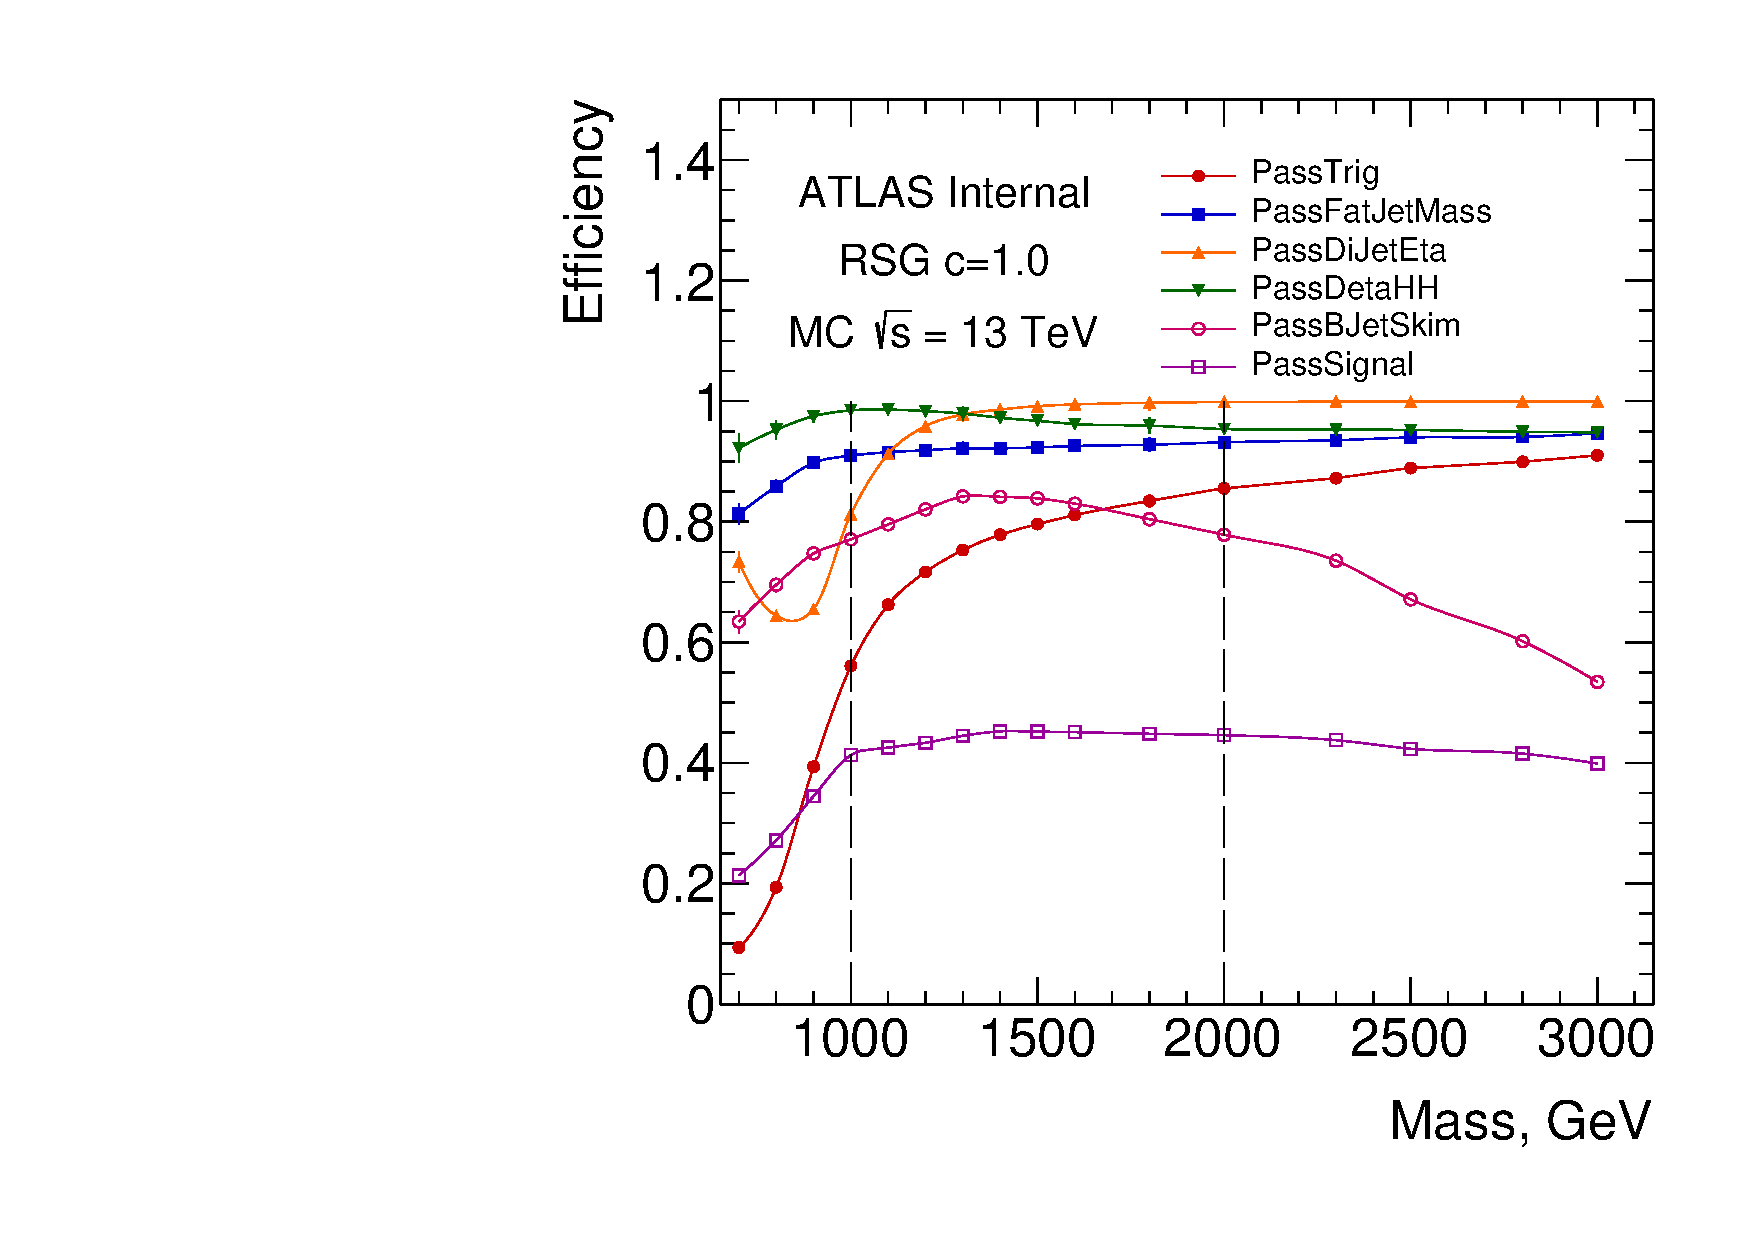
\includegraphics[width=0.48\textwidth,angle=-90]{figures/boosted/SigEff/evtsel_Moriond_Efficiency_PreSel_rel.pdf}
  \caption{Absolute (left) and relative (right) signal efficiency as a function of RSG c=1.0 signal resonance mass hypothesis for selection cuts. The relative efficiency is defined from the previous cut, where the order of cuts is given by the legend. PassTrig means the event passes the trigger selection; PassDiJetPt means the event passes the leading and sub-leading jet \pt cuts; PassDiJetEta means the event passes the leading and sub-leading jet $\eta$ cuts; PassDetaH means the events passes the $|\Delta \eta| < 1.7$ cut; PassBJetSkim means the event contains at least two $b$-tagged track jets, inclusive of $2b$, $2bs$, $3b$ and $4b$ configurations; PassSignal means the event passes the signal region cut $X_{hh} < 1.6$.}
  \label{fig:boosted-selection-efficiency}
\end{center}
\end{figure*}

\paragraph{}
The selection efficiency at various stages for \Grav with $c=1.0$, \Grav with $c=2.0$, and Heavy Scalar signal samples of all mass points can be found in Table~\ref{boosted-eff-RSG_c10}, ~\ref{boosted-eff-RSG_c20} and ~\ref{boosted-eff-2HDM}.


% \begin{figure*}
% \begin{center}
% \subfloat[]{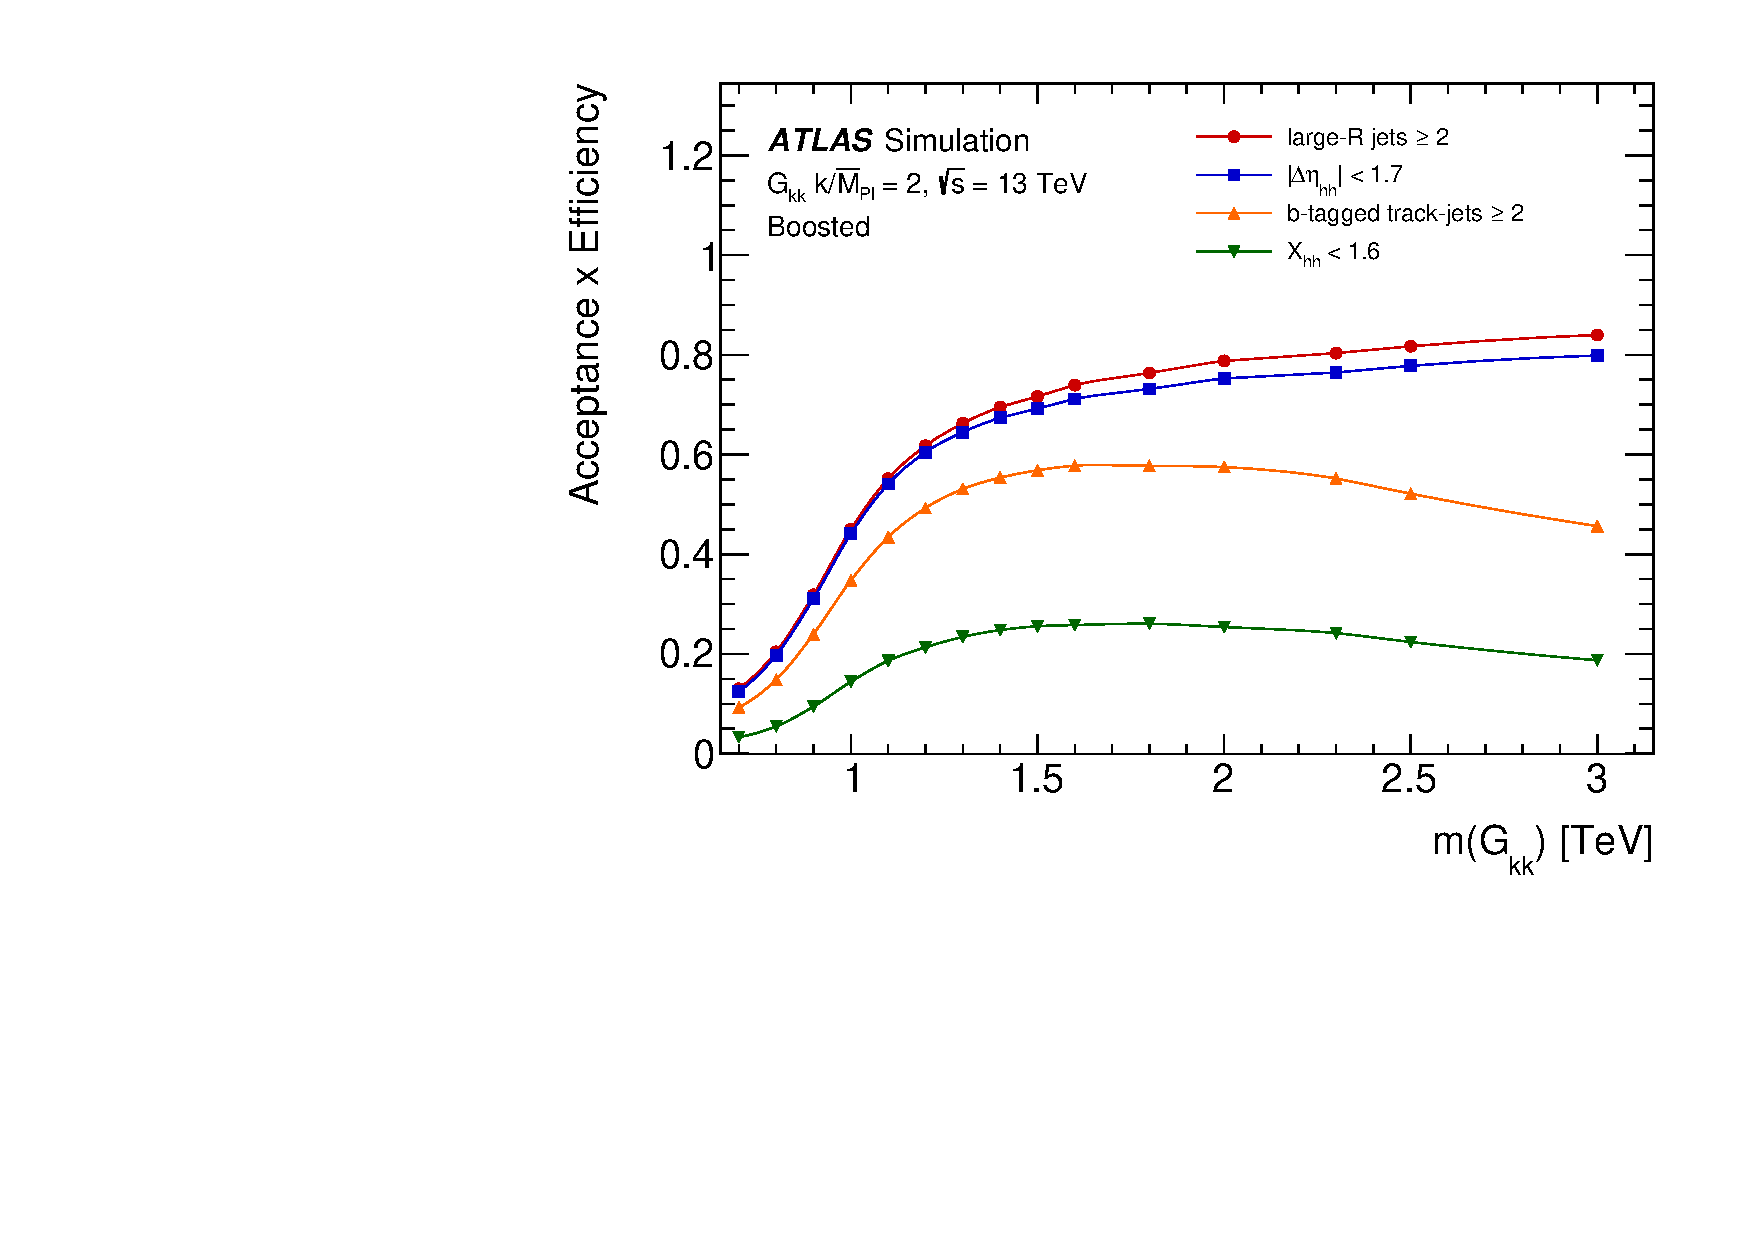
\includegraphics[width=0.48\textwidth,angle=-90]{figures/boosted/SigEff/G_hh_c20_evtsel_Moriond_bkg_9_Efficiency_PreSel.pdf}
% \subfloat[]{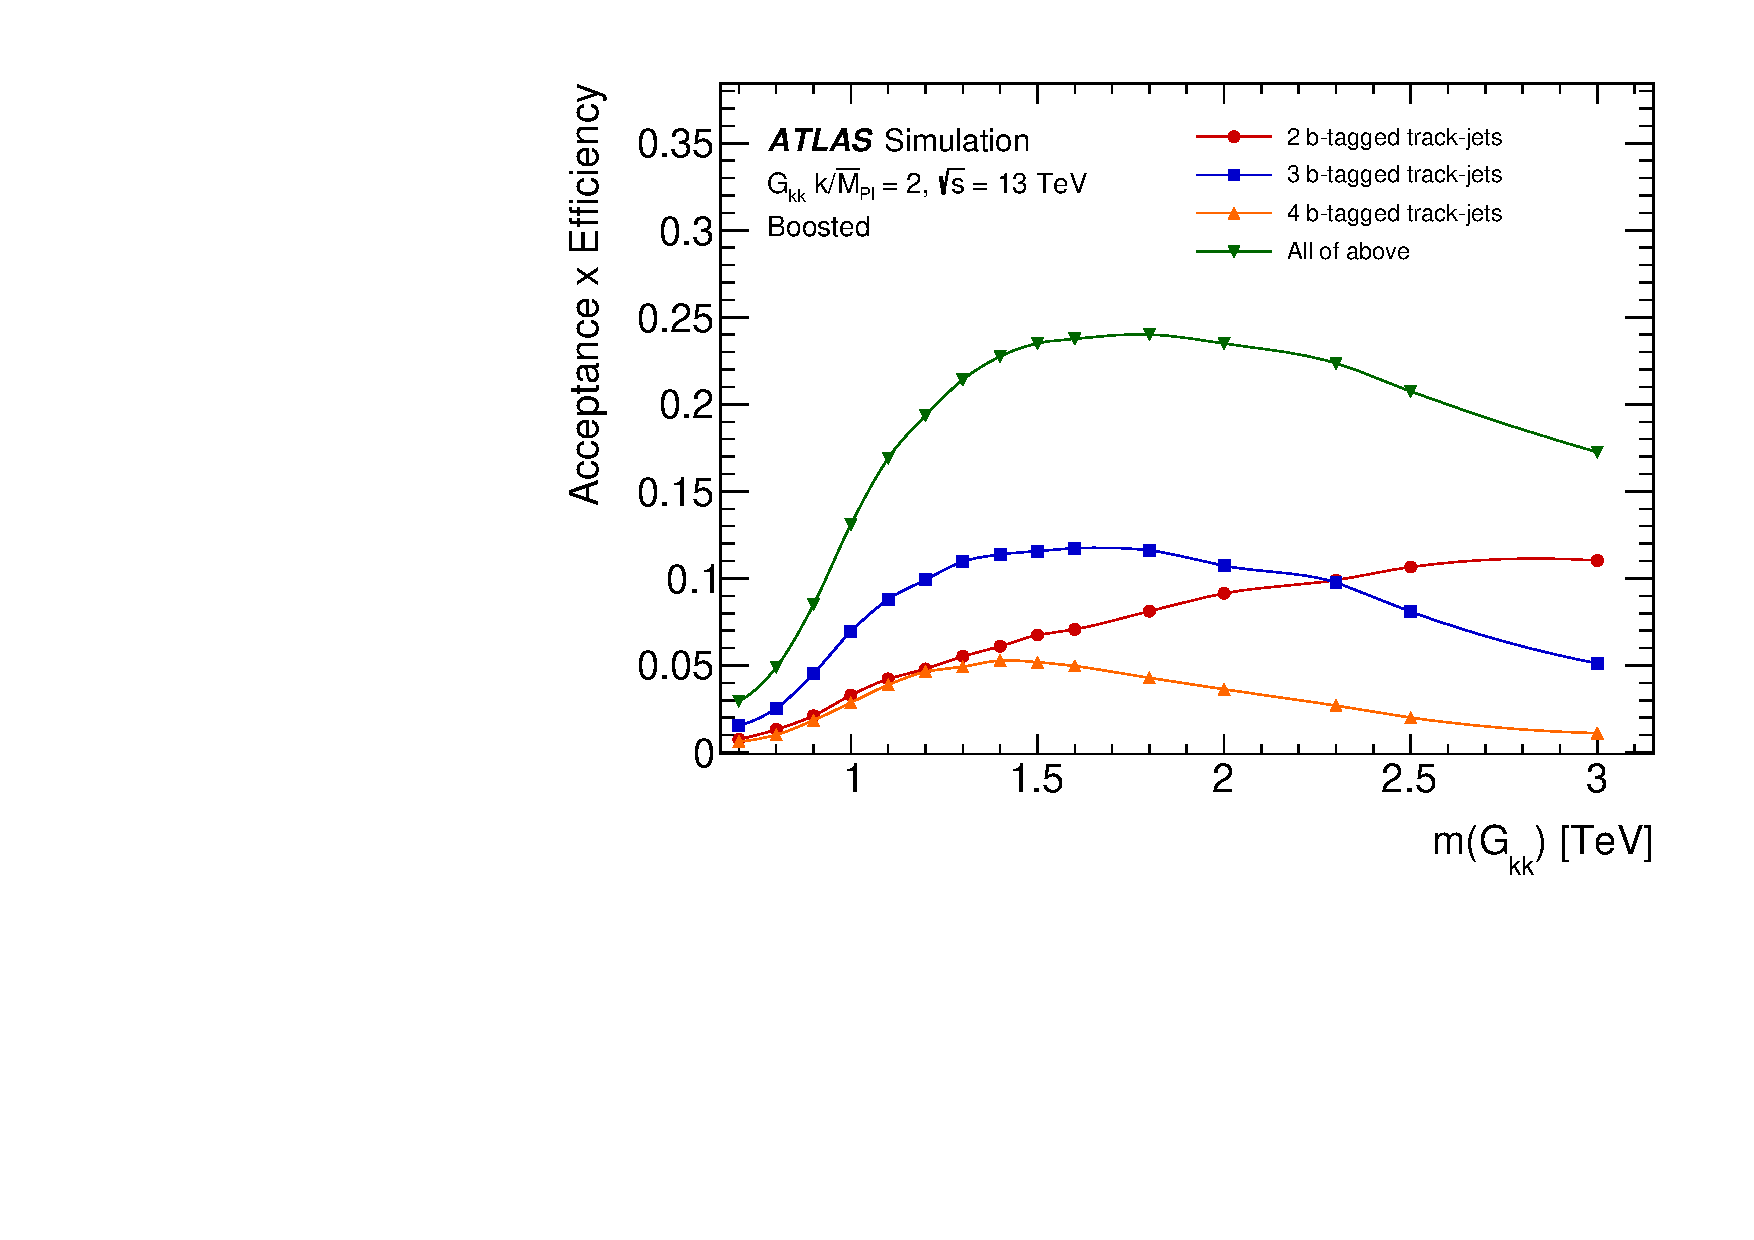
\includegraphics[width=0.48\textwidth,angle=-90]{figures/boosted/SigEff/G_hh_c20_region_lst_Moriond_bkg_9_Efficiency_PreSel.pdf}
% \caption{(a) The selection acceptance times efficiency of the boosted analysis at each stage of the event selection as a function of the generated graviton mass for $\kMPl = 2$. The trigger efficiency is approximately 100\% after the requirement of two large-\R jets, so it is not shown. (b) The selection efficiency of the three signal region samples defined by $b$-tagging requirements, as a function of the generated graviton mass for $\kMPl = 2$.}
% \end{center}
% \end{figure*}

\begin{table}[htbp!]
\scriptsize
\caption{The selection efficiency for $G_{KK}^{*}\rightarrow hh\rightarrow b\bar{b}b\bar{b}$ events ($c=1.0$) at each stage of the event selection. Uncertainties are the MC stat uncertainty only.}
\begin{center}
\resizebox{\textwidth}{!}{
\begin{footnotesize} 
\begin{tabular}{c|c|c|c|c|c|c|c} 
Resonance Mass [GeV] & Mini-ntuple Skimming & 2 large-R jets & $\Delta\eta$ & Xhh < 1.6 & 2bs SR & 3b SR & 4b SR \\ 
\hline\hline 
500 & 317.31 $\pm$ 6.0 & 295.75 $\pm$ 5.79 & 164.5 $\pm$ 4.32 & 8.45 $\pm$ 0.99 & 1.08 $\pm$ 0.37 & 2.14 $\pm$ 0.52 & 0 $\pm$ 0\\ 
600 & 269.07 $\pm$ 3.64 & 247.94 $\pm$ 3.5 & 136.31 $\pm$ 2.59 & 11.31 $\pm$ 0.76 & 2.57 $\pm$ 0.37 & 3.84 $\pm$ 0.45 & 0.66 $\pm$ 0.19\\ 
700 & 253.68 $\pm$ 3.35 & 226.93 $\pm$ 3.16 & 124.83 $\pm$ 2.35 & 16.79 $\pm$ 0.86 & 3.74 $\pm$ 0.42 & 6.99 $\pm$ 0.56 & 1.91 $\pm$ 0.29\\ 
800 & 286.26 $\pm$ 2.28 & 245.36 $\pm$ 2.11 & 129.2 $\pm$ 1.53 & 24.41 $\pm$ 0.67 & 5.11 $\pm$ 0.31 & 11.27 $\pm$ 0.46 & 4.13 $\pm$ 0.27\\ 
900 & 306.51 $\pm$ 1.61 & 275.57 $\pm$ 1.52 & 158.03 $\pm$ 1.15 & 40.72 $\pm$ 0.59 & 8.81 $\pm$ 0.28 & 19.76 $\pm$ 0.41 & 7.5 $\pm$ 0.25\\ 
1000 & 238.2 $\pm$ 0.98 & 226.98 $\pm$ 0.96 & 165.2 $\pm$ 0.82 & 52.86 $\pm$ 0.47 & 10.87 $\pm$ 0.22 & 26.0 $\pm$ 0.33 & 10.07 $\pm$ 0.2\\ 
1100 & 164.5 $\pm$ 0.63 & 160.94 $\pm$ 0.63 & 132.53 $\pm$ 0.57 & 45.26 $\pm$ 0.34 & 9.55 $\pm$ 0.16 & 21.88 $\pm$ 0.23 & 9.03 $\pm$ 0.14\\ 
1200 & 109.24 $\pm$ 0.41 & 107.92 $\pm$ 0.4 & 93.45 $\pm$ 0.38 & 33.53 $\pm$ 0.23 & 6.96 $\pm$ 0.11 & 15.8 $\pm$ 0.16 & 7.38 $\pm$ 0.1\\ 
1300 & 72.72 $\pm$ 0.59 & 72.2 $\pm$ 0.59 & 63.74 $\pm$ 0.56 & 24.19 $\pm$ 0.35 & 5.02 $\pm$ 0.17 & 11.33 $\pm$ 0.24 & 5.45 $\pm$ 0.16\\ 
1400 & 48.83 $\pm$ 0.17 & 48.61 $\pm$ 0.17 & 42.96 $\pm$ 0.16 & 16.62 $\pm$ 0.1 & 3.72 $\pm$ 0.052 & 7.61 $\pm$ 0.07 & 3.68 $\pm$ 0.046\\ 
1500 & 33.13 $\pm$ 0.12 & 33.02 $\pm$ 0.12 & 29.25 $\pm$ 0.11 & 11.31 $\pm$ 0.07 & 2.67 $\pm$ 0.036 & 5.08 $\pm$ 0.047 & 2.44 $\pm$ 0.031\\ 
1600 & 22.81 $\pm$ 0.08 & 22.75 $\pm$ 0.08 & 20.16 $\pm$ 0.075 & 7.74 $\pm$ 0.048 & 1.93 $\pm$ 0.025 & 3.48 $\pm$ 0.032 & 1.53 $\pm$ 0.02\\ 
1800 & 11.2 $\pm$ 0.1 & 11.18 $\pm$ 0.1 & 9.93 $\pm$ 0.094 & 3.71 $\pm$ 0.059 & 1.1 $\pm$ 0.034 & 1.6 $\pm$ 0.038 & 0.6 $\pm$ 0.022\\ 
2000 & 5.72 $\pm$ 0.021 & 5.71 $\pm$ 0.021 & 5.07 $\pm$ 0.019 & 1.83 $\pm$ 0.012 & 0.6 $\pm$ 0.0072 & 0.76 $\pm$ 0.0076 & 0.25 $\pm$ 0.0041\\ 
2250 & 2.61 $\pm$ 0.0088 & 2.61 $\pm$ 0.0088 & 2.32 $\pm$ 0.0083 & 0.78 $\pm$ 0.005 & 0.31 $\pm$ 0.0032 & 0.3 $\pm$ 0.003 & 0.078 $\pm$ 0.0014\\ 
2500 & 1.24 $\pm$ 0.0054 & 1.24 $\pm$ 0.0054 & 1.11 $\pm$ 0.0051 & 0.33 $\pm$ 0.0028 & 0.16 $\pm$ 0.002 & 0.11 $\pm$ 0.0016 & 0.021 $\pm$ 0.00066\\ 
2750 & 0.6 $\pm$ 0.0026 & 0.6 $\pm$ 0.0026 & 0.54 $\pm$ 0.0025 & 0.14 $\pm$ 0.0013 & 0.081 $\pm$ 0.00099 & 0.038 $\pm$ 0.00065 & 0.0055 $\pm$ 0.00024\\ 
3000 & 0.3 $\pm$ 0.0011 & 0.3 $\pm$ 0.0011 & 0.27 $\pm$ 0.0011 & 0.058 $\pm$ 0.00051 & 0.039 $\pm$ 0.00041 & 0.013 $\pm$ 0.00023 & 0.0016 $\pm$ 8e-05\\ 
\hline\hline 
\end{tabular} 
\end{footnotesize} 
\newline 

}
\end{center}
\label{boosted-eff-RSG_c10}
\end{table}

\begin{table}[htbp!]
\scriptsize
\caption{The selection efficiency for $G_{KK}^{*}\rightarrow hh\rightarrow b\bar{b}b\bar{b}$ events ($c=2.0$) at each stage of the event selection. Uncertainties are the MC stat uncertainty only.}
\begin{center}
\resizebox{\textwidth}{!}{
\begin{footnotesize} 
\begin{tabular}{c|c|c|c|c|c|c|c} 
Resonance Mass [GeV] & Mini-ntuple Skimming & 2 large-R jets & $\Delta\eta$ & Xhh < 1.6 & 2bs SR & 3b SR & 4b SR \\ 
\hline\hline 
500 & 3705.15 $\pm$ 40.86 & 3479.44 $\pm$ 39.59 & 2325.18 $\pm$ 32.37 & 568.04 $\pm$ 16.17 & 122.56 $\pm$ 7.76 & 253.49 $\pm$ 10.78 & 100.7 $\pm$ 6.53\\ 
600 & 2549.14 $\pm$ 22.55 & 2374.01 $\pm$ 21.76 & 1591.92 $\pm$ 17.82 & 396.96 $\pm$ 9.03 & 89.01 $\pm$ 4.46 & 178.63 $\pm$ 6.05 & 74.31 $\pm$ 3.71\\ 
700 & 1928.4 $\pm$ 13.57 & 1782.85 $\pm$ 13.04 & 1183.86 $\pm$ 10.63 & 320.53 $\pm$ 5.62 & 71.38 $\pm$ 2.76 & 148.41 $\pm$ 3.81 & 59.31 $\pm$ 2.31\\ 
800 & 1595.14 $\pm$ 8.82 & 1457.71 $\pm$ 8.43 & 958.89 $\pm$ 6.84 & 268.75 $\pm$ 3.67 & 64.14 $\pm$ 1.86 & 123.48 $\pm$ 2.47 & 49.43 $\pm$ 1.51\\ 
900 & 1264.78 $\pm$ 5.77 & 1179.88 $\pm$ 5.58 & 819.75 $\pm$ 4.65 & 251.29 $\pm$ 2.61 & 55.63 $\pm$ 1.27 & 119.44 $\pm$ 1.79 & 48.72 $\pm$ 1.11\\ 
1000 & 891.0 $\pm$ 3.66 & 856.95 $\pm$ 3.59 & 662.54 $\pm$ 3.15 & 219.04 $\pm$ 1.84 & 49.45 $\pm$ 0.91 & 104.31 $\pm$ 1.26 & 42.97 $\pm$ 0.78\\ 
1100 & 595.58 $\pm$ 2.98 & 581.72 $\pm$ 2.95 & 481.67 $\pm$ 2.68 & 167.96 $\pm$ 1.61 & 37.64 $\pm$ 0.79 & 78.28 $\pm$ 1.09 & 34.59 $\pm$ 0.7\\ 
1200 & 390.84 $\pm$ 1.69 & 385.41 $\pm$ 1.68 & 330.23 $\pm$ 1.55 & 118.0 $\pm$ 0.94 & 26.23 $\pm$ 0.46 & 54.18 $\pm$ 0.64 & 25.34 $\pm$ 0.42\\ 
1300 & 257.66 $\pm$ 0.94 & 255.35 $\pm$ 0.94 & 222.37 $\pm$ 0.88 & 82.11 $\pm$ 0.54 & 19.04 $\pm$ 0.27 & 37.8 $\pm$ 0.37 & 16.99 $\pm$ 0.23\\ 
1400 & 172.09 $\pm$ 0.72 & 171.02 $\pm$ 0.71 & 150.22 $\pm$ 0.67 & 56.23 $\pm$ 0.42 & 13.6 $\pm$ 0.22 & 25.36 $\pm$ 0.28 & 11.78 $\pm$ 0.18\\ 
1500 & 116.25 $\pm$ 0.41 & 115.72 $\pm$ 0.41 & 101.92 $\pm$ 0.39 & 38.5 $\pm$ 0.24 & 9.94 $\pm$ 0.13 & 17.04 $\pm$ 0.16 & 7.64 $\pm$ 0.1\\ 
1600 & 80.09 $\pm$ 0.28 & 79.82 $\pm$ 0.28 & 70.48 $\pm$ 0.26 & 26.24 $\pm$ 0.16 & 7.01 $\pm$ 0.09 & 11.62 $\pm$ 0.11 & 4.92 $\pm$ 0.067\\ 
1800 & 38.99 $\pm$ 0.14 & 38.9 $\pm$ 0.14 & 34.39 $\pm$ 0.13 & 12.65 $\pm$ 0.081 & 3.82 $\pm$ 0.047 & 5.46 $\pm$ 0.053 & 2.02 $\pm$ 0.03\\ 
2000 & 19.94 $\pm$ 0.088 & 19.91 $\pm$ 0.088 & 17.68 $\pm$ 0.083 & 6.17 $\pm$ 0.05 & 2.15 $\pm$ 0.031 & 2.52 $\pm$ 0.032 & 0.85 $\pm$ 0.017\\ 
2250 & 9.02 $\pm$ 0.031 & 9.01 $\pm$ 0.031 & 7.99 $\pm$ 0.029 & 2.62 $\pm$ 0.017 & 1.03 $\pm$ 0.011 & 1.02 $\pm$ 0.01 & 0.28 $\pm$ 0.0051\\ 
2500 & 4.28 $\pm$ 0.016 & 4.28 $\pm$ 0.016 & 3.8 $\pm$ 0.015 & 1.13 $\pm$ 0.0083 & 0.52 $\pm$ 0.0058 & 0.4 $\pm$ 0.0048 & 0.098 $\pm$ 0.0022\\ 
3000 & 1.07 $\pm$ 0.004 & 1.07 $\pm$ 0.004 & 0.96 $\pm$ 0.0038 & 0.23 $\pm$ 0.0019 & 0.13 $\pm$ 0.0015 & 0.062 $\pm$ 0.00097 & 0.013 $\pm$ 0.00043\\ 
\hline\hline 
\end{tabular} 
\end{footnotesize} 
\newline 

}
\end{center}
\label{boosted-eff-RSG_c20}
\end{table}

\begin{table}[htbp!]
\scriptsize
\caption{The selection efficiency for $H\rightarrow hh\rightarrow b\bar{b}b\bar{b}$ events at each stage of the event selection.}
\begin{center}
\resizebox{\textwidth}{!}{
\begin{footnotesize} 
\begin{tabular}{c|c|c|c|c|c|c|c} 
Resonance Mass [GeV] & Mini-ntuple Skimming & 2 large-R jets & $\Delta\eta$ & Xhh < 1.6 & 2bs SR & 3b SR & 4b SR \\ 
\hline\hline 
500 & 1557.94 $\pm$ 136.12 & 1022.77 $\pm$ 110.29 & 95.14 $\pm$ 33.64 & 11.69 $\pm$ 11.69 & 0 $\pm$ 0 & 11.69 $\pm$ 11.69 & 0 $\pm$ 0\\ 
600 & 3289.78 $\pm$ 123.99 & 2542.11 $\pm$ 108.99 & 485.99 $\pm$ 47.66 & 54.55 $\pm$ 15.77 & 18.73 $\pm$ 9.39 & 9.17 $\pm$ 6.49 & 0 $\pm$ 0\\ 
700 & 4655.21 $\pm$ 94.59 & 3855.64 $\pm$ 86.09 & 1237.8 $\pm$ 48.78 & 142.42 $\pm$ 17.03 & 28.55 $\pm$ 7.74 & 52.6 $\pm$ 10.75 & 7.69 $\pm$ 3.85\\ 
800 & 7506.31 $\pm$ 81.79 & 6020.56 $\pm$ 73.25 & 2150.64 $\pm$ 43.78 & 320.63 $\pm$ 17.02 & 67.63 $\pm$ 7.83 & 139.97 $\pm$ 11.23 & 47.57 $\pm$ 6.75\\ 
900 & 9732.89 $\pm$ 61.17 & 8400.91 $\pm$ 56.83 & 3574.63 $\pm$ 37.07 & 806.13 $\pm$ 17.76 & 188.71 $\pm$ 8.71 & 377.92 $\pm$ 12.12 & 127.7 $\pm$ 6.99\\ 
1000 & 7516.07 $\pm$ 37.72 & 7033.18 $\pm$ 36.49 & 4496.85 $\pm$ 29.18 & 1351.1 $\pm$ 16.2 & 303.71 $\pm$ 7.88 & 650.89 $\pm$ 11.19 & 234.2 $\pm$ 6.57\\ 
1100 & 4731.39 $\pm$ 21.54 & 4563.4 $\pm$ 21.15 & 3485.58 $\pm$ 18.49 & 1135.18 $\pm$ 10.7 & 251.77 $\pm$ 5.18 & 539.51 $\pm$ 7.36 & 215.39 $\pm$ 4.5\\ 
1200 & 2853.51 $\pm$ 12.23 & 2782.42 $\pm$ 12.07 & 2253.95 $\pm$ 10.87 & 786.92 $\pm$ 6.53 & 175.53 $\pm$ 3.21 & 366.01 $\pm$ 4.44 & 158.29 $\pm$ 2.8\\ 
1300 & 1700.83 $\pm$ 7.01 & 1668.05 $\pm$ 6.94 & 1362.91 $\pm$ 6.27 & 494.36 $\pm$ 3.84 & 107.0 $\pm$ 1.86 & 224.19 $\pm$ 2.58 & 107.55 $\pm$ 1.7\\ 
1400 & 1016.14 $\pm$ 4.03 & 999.98 $\pm$ 4.0 & 802.44 $\pm$ 3.59 & 296.46 $\pm$ 2.22 & 65.49 $\pm$ 1.1 & 133.86 $\pm$ 1.49 & 65.58 $\pm$ 0.99\\ 
1500 & 621.34 $\pm$ 2.41 & 613.46 $\pm$ 2.39 & 484.92 $\pm$ 2.13 & 179.29 $\pm$ 1.32 & 42.75 $\pm$ 0.68 & 79.32 $\pm$ 0.88 & 36.77 $\pm$ 0.56\\ 
1600 & 386.3 $\pm$ 1.46 & 382.44 $\pm$ 1.46 & 297.63 $\pm$ 1.28 & 109.99 $\pm$ 0.8 & 27.68 $\pm$ 0.42 & 49.3 $\pm$ 0.53 & 20.92 $\pm$ 0.32\\ 
1800 & 154.8 $\pm$ 0.58 & 153.5 $\pm$ 0.57 & 116.52 $\pm$ 0.5 & 42.24 $\pm$ 0.31 & 12.41 $\pm$ 0.18 & 18.2 $\pm$ 0.2 & 6.66 $\pm$ 0.11\\ 
2000 & 65.4 $\pm$ 0.24 & 65.02 $\pm$ 0.24 & 48.57 $\pm$ 0.2 & 16.89 $\pm$ 0.12 & 5.64 $\pm$ 0.076 & 7.01 $\pm$ 0.079 & 2.18 $\pm$ 0.041\\ 
2250 & 23.84 $\pm$ 0.085 & 23.73 $\pm$ 0.085 & 17.44 $\pm$ 0.073 & 5.57 $\pm$ 0.042 & 2.25 $\pm$ 0.028 & 2.11 $\pm$ 0.025 & 0.52 $\pm$ 0.012\\ 
2500 & 9.2 $\pm$ 0.032 & 9.17 $\pm$ 0.032 & 6.72 $\pm$ 0.028 & 1.9 $\pm$ 0.015 & 0.92 $\pm$ 0.011 & 0.64 $\pm$ 0.0086 & 0.11 $\pm$ 0.0034\\ 
2750 & 3.73 $\pm$ 0.013 & 3.73 $\pm$ 0.013 & 2.71 $\pm$ 0.011 & 0.63 $\pm$ 0.0054 & 0.37 $\pm$ 0.0042 & 0.17 $\pm$ 0.0027 & 0.021 $\pm$ 0.00093\\ 
3000 & 1.59 $\pm$ 0.0054 & 1.59 $\pm$ 0.0054 & 1.15 $\pm$ 0.0046 & 0.22 $\pm$ 0.0021 & 0.15 $\pm$ 0.0017 & 0.044 $\pm$ 0.0009 & 0.0038 $\pm$ 0.00025\\ 
\hline\hline 
\end{tabular} 
\end{footnotesize} 
\newline 

}
\end{center}
\label{boosted-eff-2HDM}
\end{table}


% \paragraph{}
% To improve the analysis, a quantity which defines the sensitivity of analysis is maximized. Techicially, the optimal sensitivity is described as $\sqrt{2((S+B)\ln{1 + \frac{S}{B}} - S}$, see \href{https://www.pp.rhul.ac.uk/~cowan/stat/notes/SigCalcNote.pdf}{note}. This is usually considered at the $S << B$ limit and simplified as $\frac{S}{\sqrt{B}}$, when no knowledge of the model cross section is available, or $\frac{S}{\sqrt{S + B}}$, if the signal cross section is known. These parametrizations have limitations, particularly when the signal yield and the number of estiamted background are both small. A better parametrization for low signal strengh is $\frac{S}{\sqrt{1 + B}}$, where the extra $\sqrt{1 + B}$ accounts for poisson fluctuations. For a discussion of p-values, please see this \href{https://arxiv.org/pdf/hep-ex/0208005.pdf}{note}.

% \paragraph{}
% For this analysis, two methods are used: one is calculate the number of signal and backgrounds within $68\%$ of the signal \mhh mass window, the other is to implement the full signal and background predicions after smoothing and compare the asymptotic expected exclusion limits. Both methods yield comparable results.
%Event Selection
%!TEX root = ../dissertation.tex
\begin{savequote}[75mm]
Even in the darkest night. Stars and angels still shine bright.   
\qauthor{Bear}
\end{savequote}


\chapter{Background Estimation}
\section{Background Estimation}
\label{sec:backgrounds}
%use the internal note structure

\paragraph{}
A similar circular variable can be defined in the two-dimensional mass plane, $R_{hh}$. The circular region $R_{hh}$ has the same central values as $X_{hh}$, but without resolution terms in the denominators and is defined as:
\begin{equation}
\label{eq:boosted_RhhDef}
R_{hh} = \sqrt{\left(m^{\rm lead}_{\rm J} - \text{124 GeV}\right)^2 + \left(m^{\rm subl}_{\rm J} - \text{115 GeV}\right)^2}
\end{equation}
The region defined by $1.6 < X_{hh}$ and $R_{hh} < 33$ is the control region. It will be discussed in Section~\ref{sec:boosted-qcd}.
The cut value was optimized to allow for a reasonable sized sample (twice the statistics as the signal region) in the control region with kinematics similar to the signal region, and avoiding the large contributions of the \ttbar~ sample when the large-\R jets have a mass near the top quark mass (with $m_J > 160$~\GeV).

\paragraph{}
Similarly, $R_{hh}^{\text{high}}$, the circular region that has the shifted central values up by 10 $GeV$ is defined using the variable:\begin{equation}
\label{eq:boosted_RhhhighDef}
R_{hh}^{\text{high}} = \sqrt{\left(m^{\rm lead}_{\rm J} - \text{134 GeV}\right)^2 + \left(m^{\rm subl}_{\rm J} - \text{125 GeV}\right)^2}
\end{equation}

\paragraph{}
In Run-1, and in the the 2015 analysis, the sideband was defined to be all events not in the signal or control regions. However, the kinematics of events with very large and very small large-R jet masses may not be the same as those within the signal region.
To avoid biasing effects from extremely low mass or extremely high mass large-$R$ jets, the sideband region is also redesigned to be like the control region, but at $R_{hh} > 33$ and $R_{hh}^{\text{high}} < 58$.
The shift upwards helps to capture enough $t\bar{t}$ events in the normalization estimates, as described in Section ~\ref{sec:ttbarnorm}.

%%\paragraph{}
The values of the $X_{hh}$ and $R_{hh}$ variables can be seen graphically in Figure~\ref{fig:boosted-regiondef-cartoons}.
\begin{figure}[htbp!]
\begin{center}
  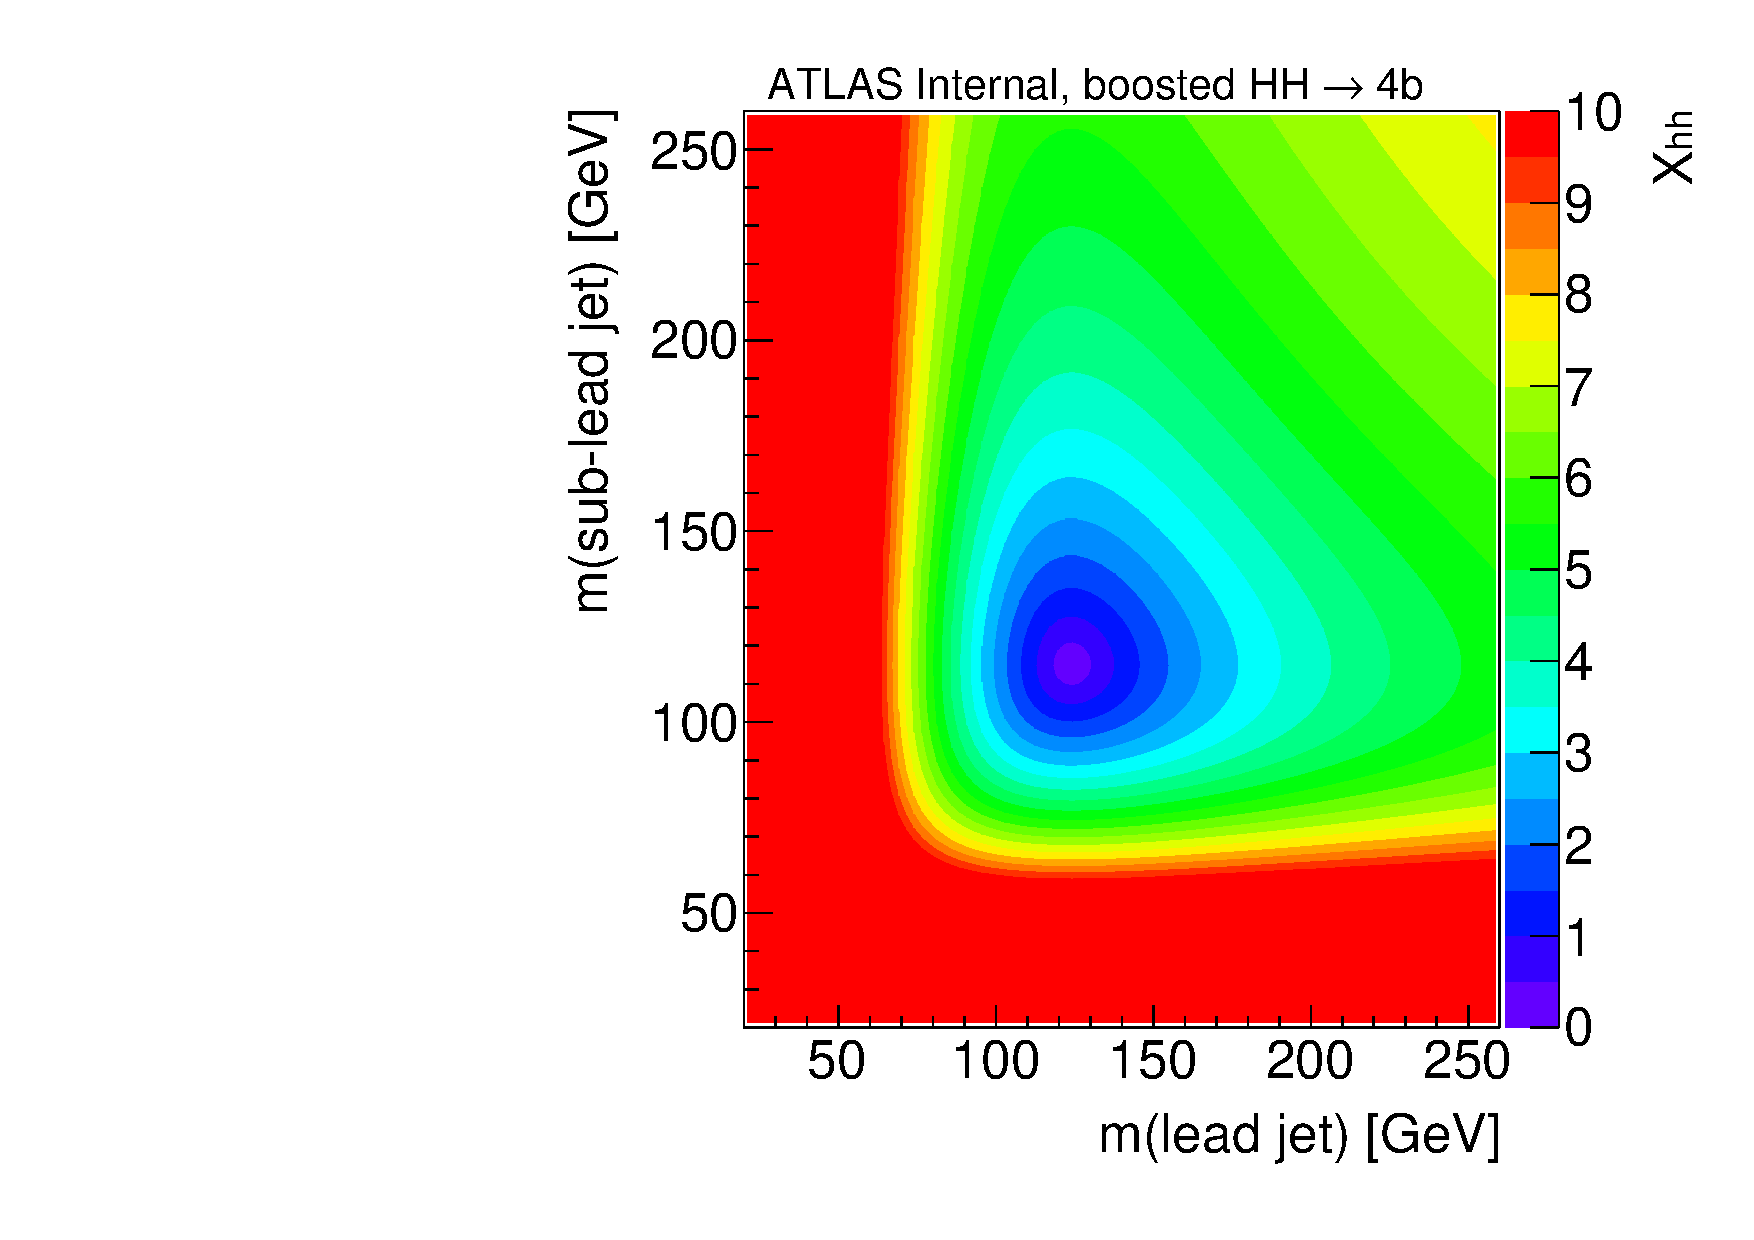
\includegraphics[width=0.45\textwidth,angle=-90]{figures/boosted/Other/cartoon-xhh.pdf}
  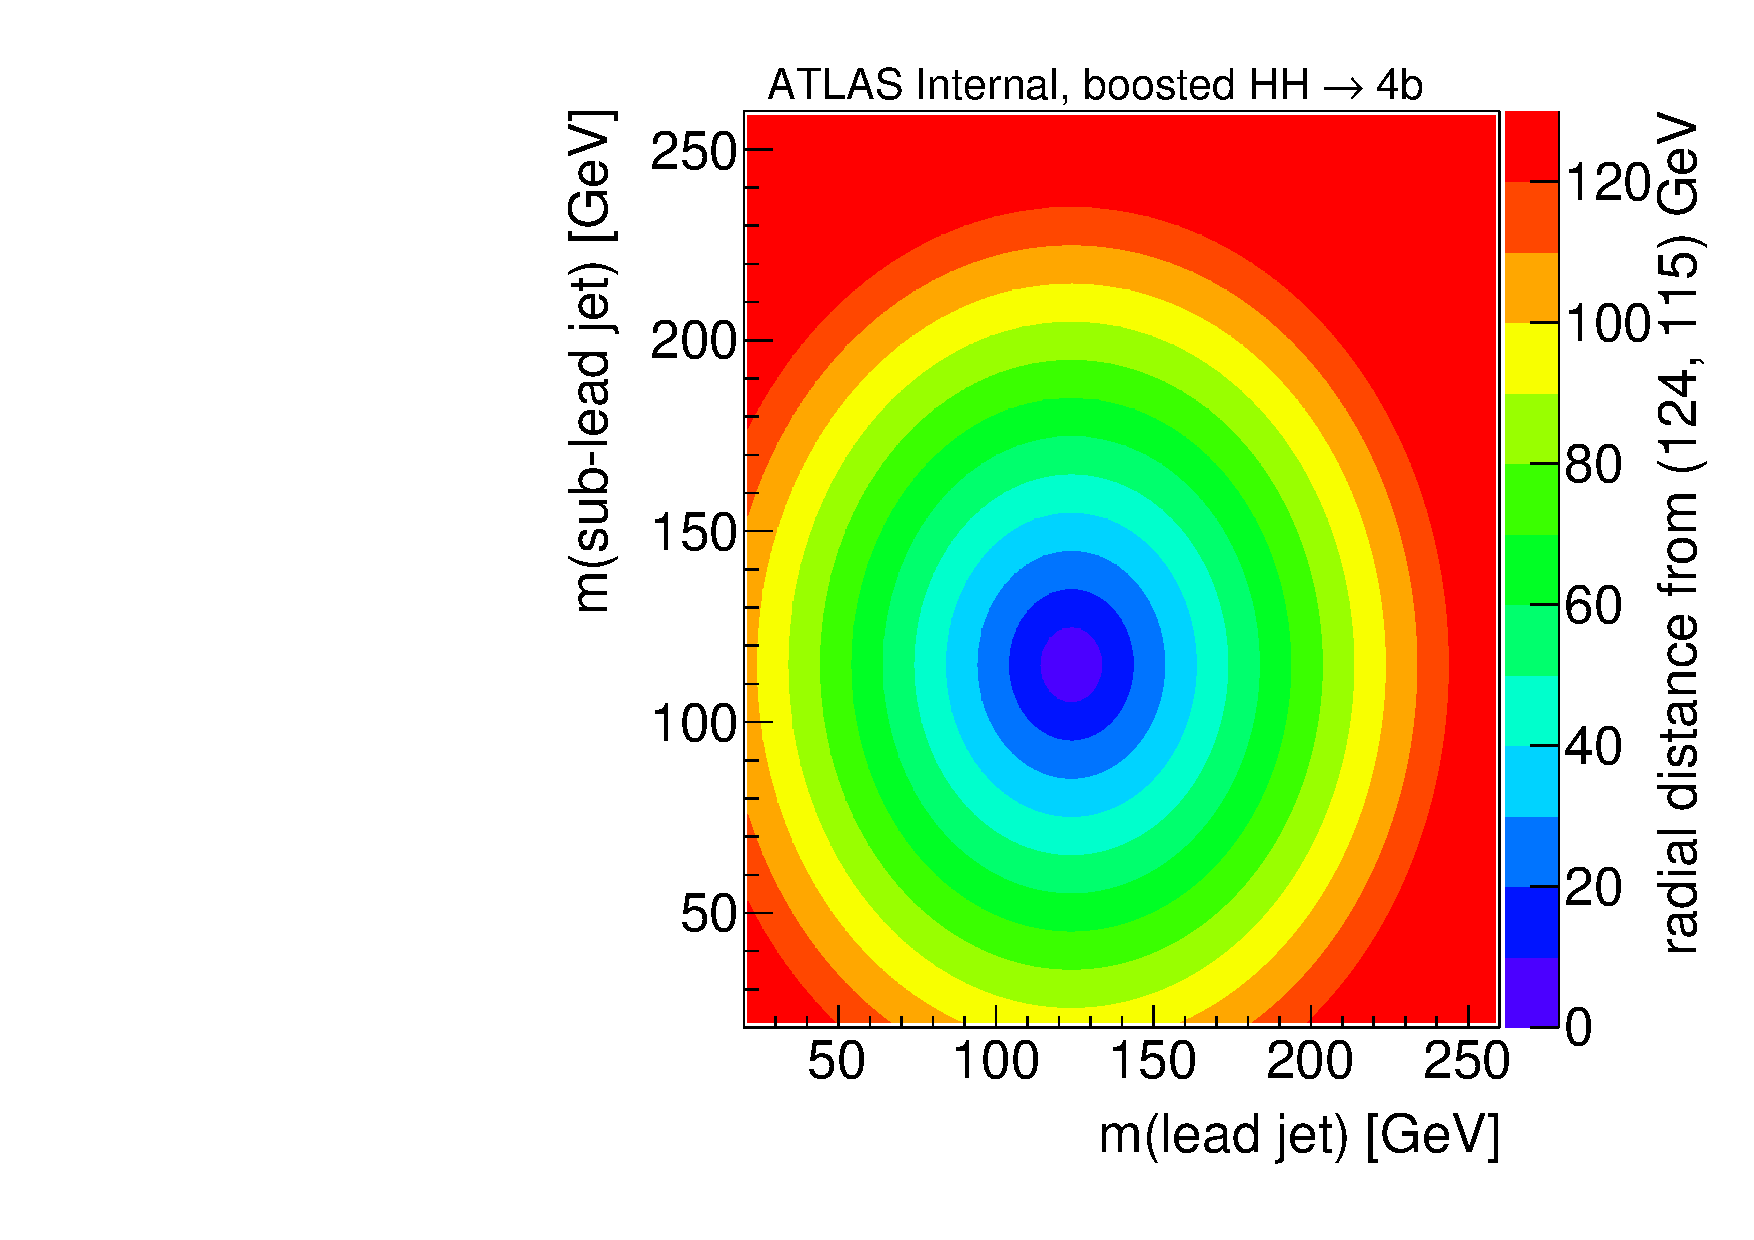
\includegraphics[width=0.45\textwidth,angle=-90]{figures/boosted/Other/cartoon-rhh.pdf}
  \caption{Values of the $X_{hh}$ and $R_{hh}$ variables, which are shapes in the two-dimensional plane of the large-R jet masses used to defined signal, control, and sideband regions. For both variables, a smaller value indicates the jets are closer to the Higgs mass. }
  \label{fig:boosted-regiondef-cartoons}
\end{center}
\end{figure}

The number of events in the control region and sideband region as a function of Resonance mass is shown in Figure~\ref{fig:boosted-selection-region-efficiency}. For 2$b$s, 3$b$ and 4$b$, each region has the number of events decrease from signal region to control region to sideband regions.

\begin{figure*}
\begin{center}
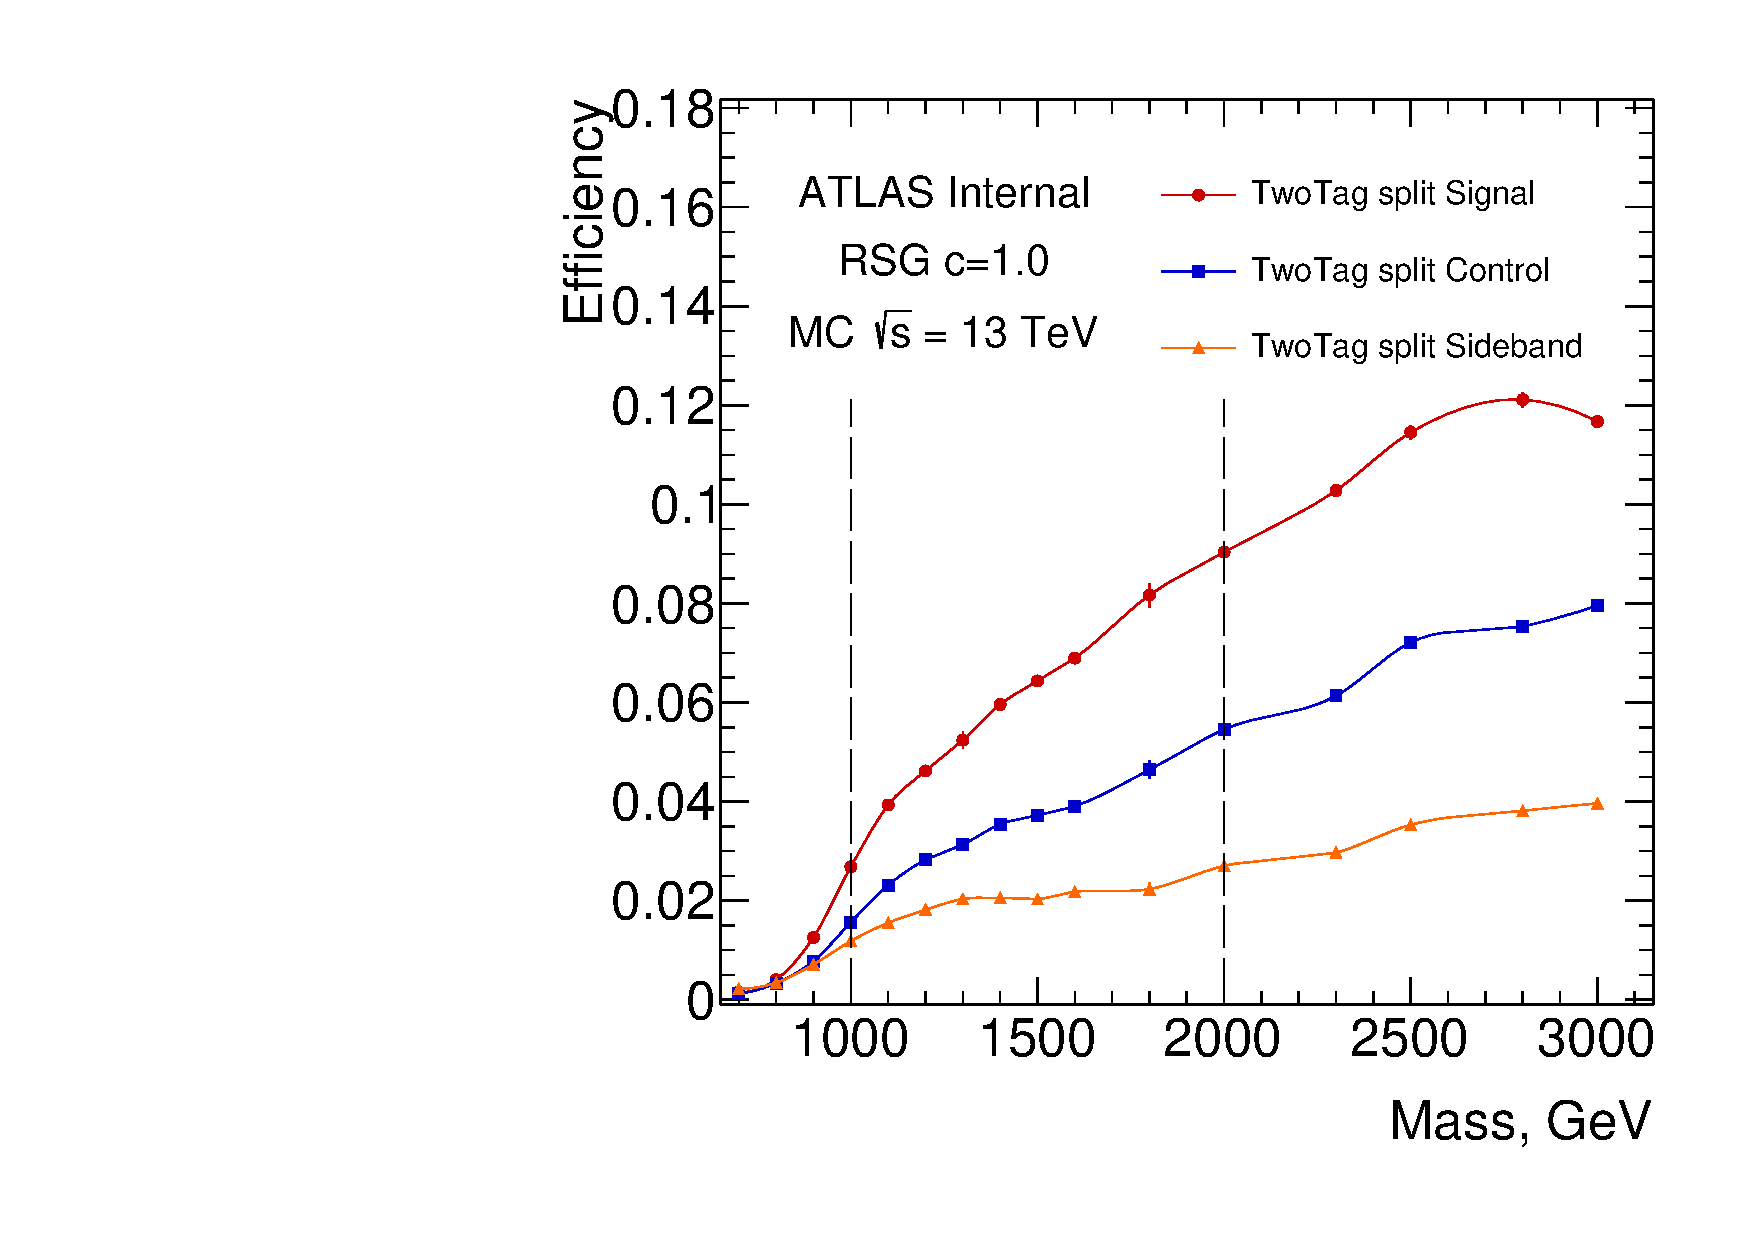
\includegraphics[width=0.48\textwidth,angle=-90]{figures/boosted/SigEff/region_2b_lst_Moriond_Efficiency_PreSel.pdf}
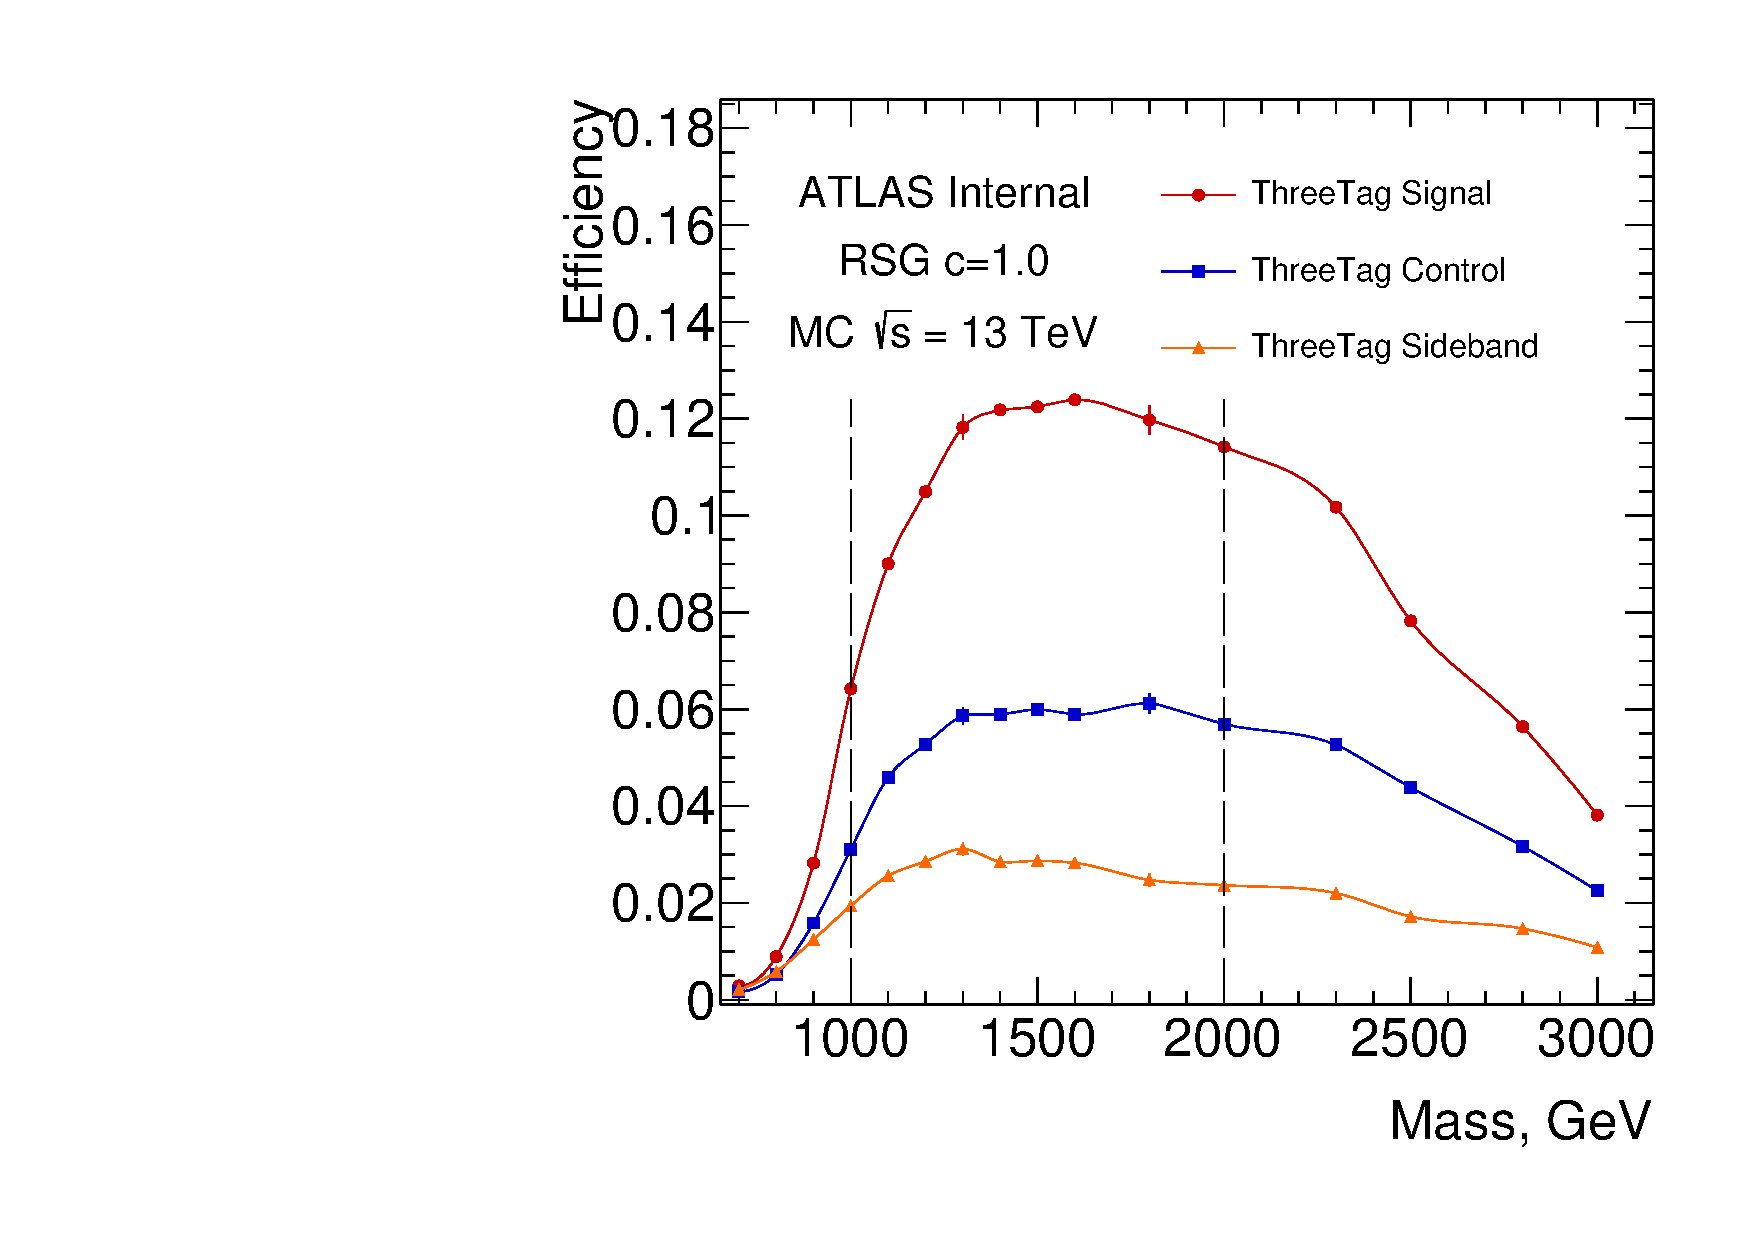
\includegraphics[width=0.48\textwidth,angle=-90]{figures/boosted/SigEff/region_3b_lst_Moriond_Efficiency_PreSel.pdf} \\
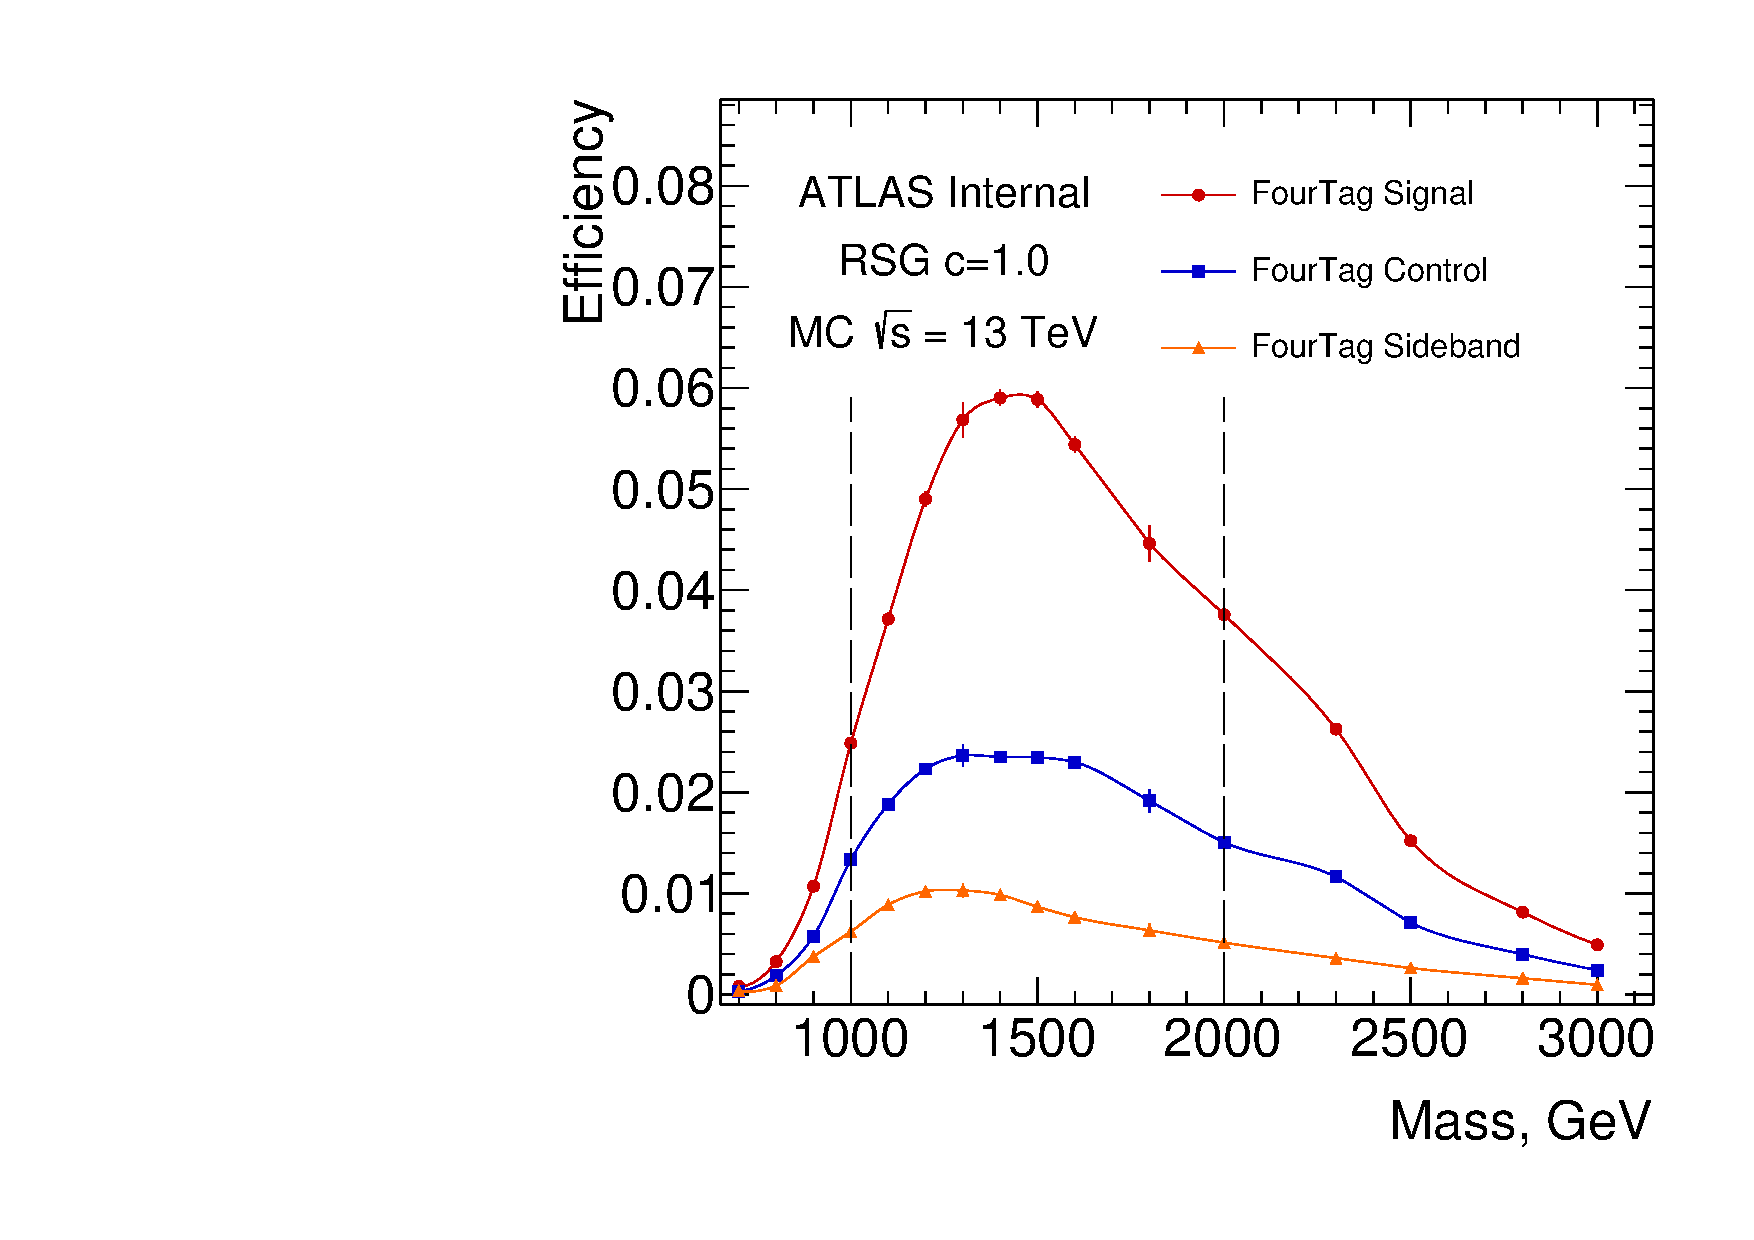
\includegraphics[width=0.48\textwidth,angle=-90]{figures/boosted/SigEff/region_4b_lst_Moriond_Efficiency_PreSel.pdf}
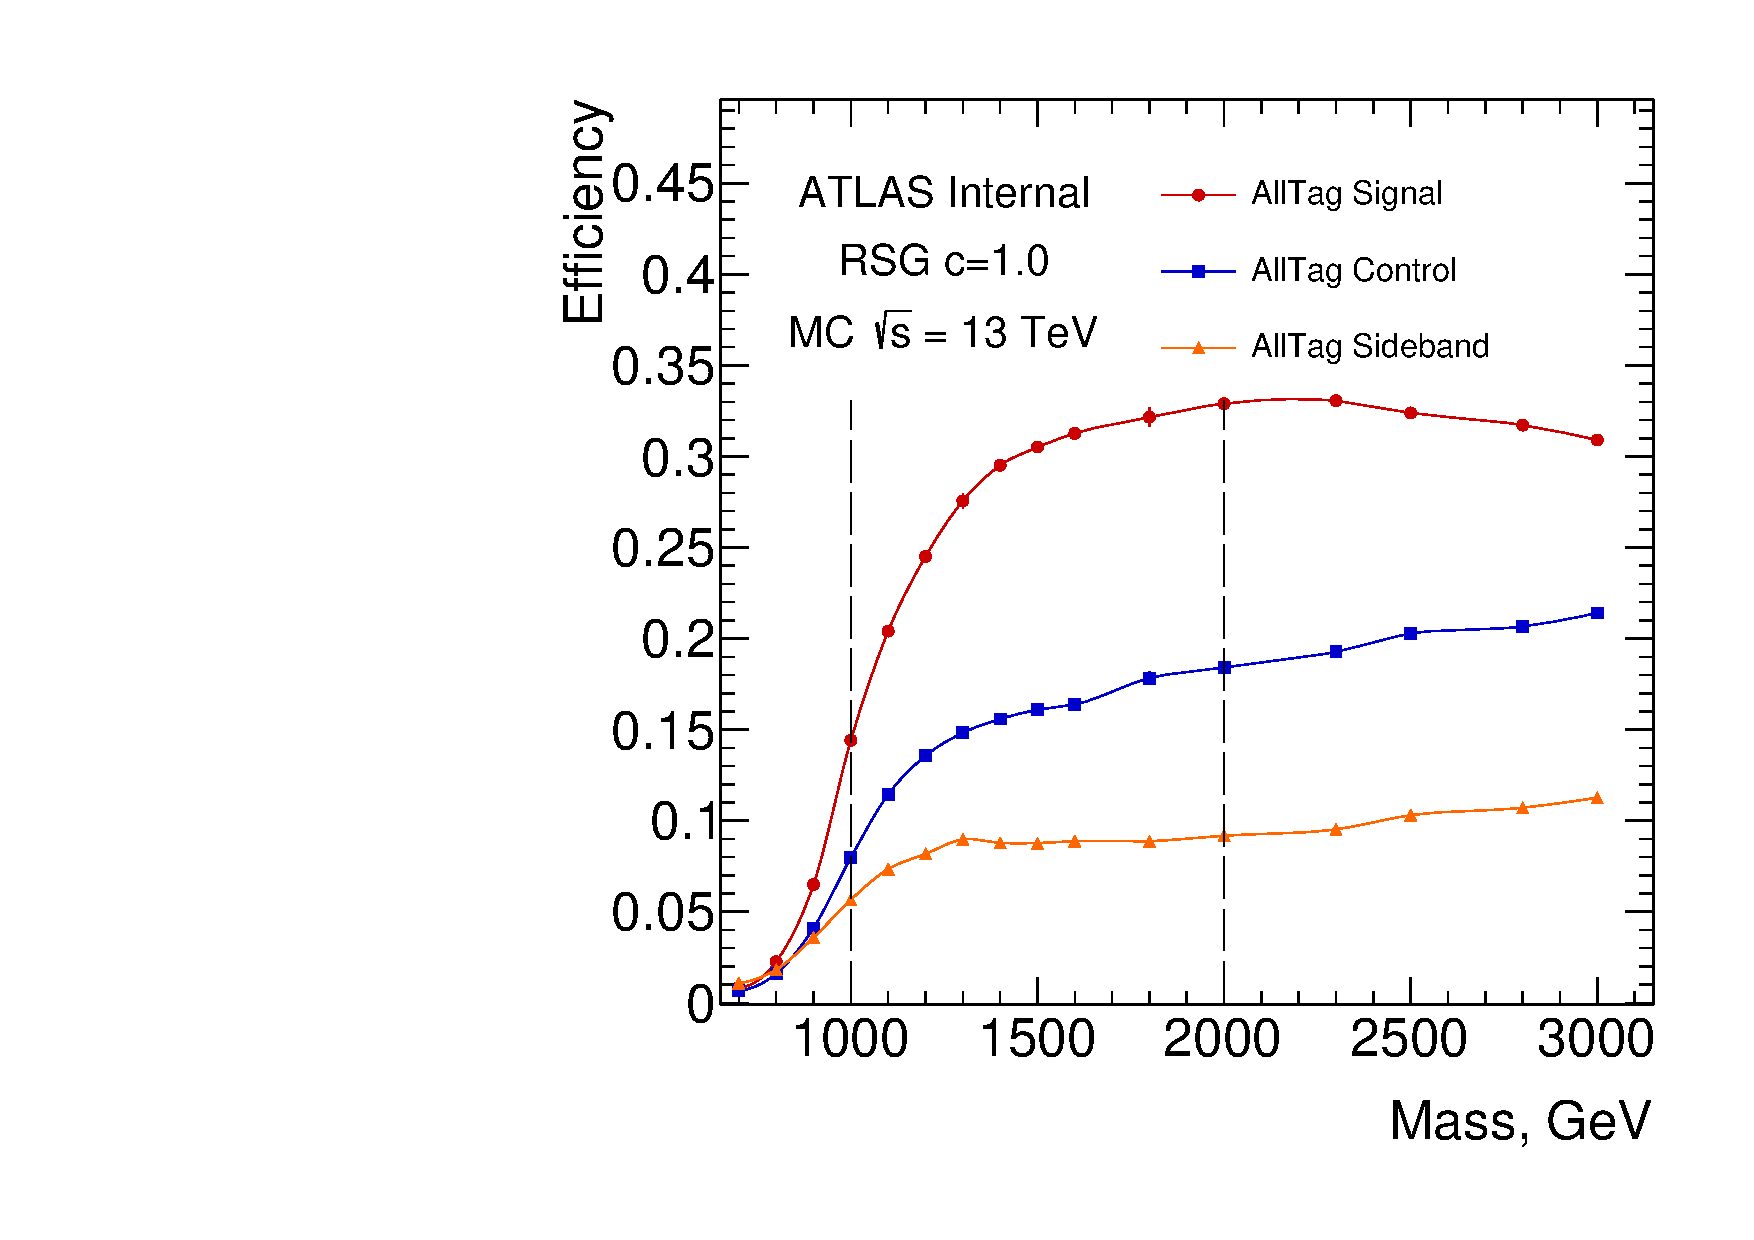
\includegraphics[width=0.48\textwidth,angle=-90]{figures/boosted/SigEff/region_alltag_lst_Moriond_Efficiency_PreSel.pdf} \\
  \caption{Detailed signal efficiency in different signal/control/sideband regions as in 2$b$s (top left, 3$b$ (top right), 4$b$ (bottom left) and inclusive b-tagged regions, which incluse 2$b$, 1$b$ and 0$b$ as well, (bottom right) as a function of signal resonance mass hypothesis for selection cuts. The efficiencies are relative to the total number of events in the preselection.}
  \label{fig:boosted-selection-region-efficiency}
\end{center}
\end{figure*}


%updated June 6 2017

\subsection{Overview}

\paragraph{}
The primary backgrounds to this analysis in the four $b$-jet signal region, in order of size, are QCD multi-jet production ($\sim 95\%$), $t\bar{t}$ ($\sim 5\%$), and $Z$+jets ($< 1\%$), where the percentages are the expected fraction of the background coming from each source. In the three $b$-jet signal region, the fractions are QCD ($\sim 90\%$), $t\bar{t}$ ($\sim 10\%$), and $Z$+jets ($< 1\%$).  In the two $b$-jet split signal region, the fractions are QCD ($\sim 80\%$), $t\bar{t}$ ($\sim 20\%$), and $Z$+jets ($< 1\%$).

\paragraph{}
QCD is by far the dominant background. However, there is no reliable, high-statistics Monte Carlo simulation sample in this region of phase space (i.e with three or four $b$-jets collected into two high-$p_{T}$ large radius jets) and thus a data-driven background estimation is needed. (See Appendix ~\ref{app:muqcd-study}.) For the \ttbar background, Monte Carlo simulation samples of reasonable size are available, and thus can be used to guide an estimation of this background. The $Z$+jets background is small enough that we will rely on the Monte Carlo simulation of $Z$+heavy flavor jets. $ZZ\to b\bar{b}b\bar{b}$ has been estimated to be completely negligible using a particle-level analysis, with less than one event expected after three $b$-tags are required, which will be further heavily suppressed by the $X_{hh}$ requirement.

\paragraph{}
The QCD background prediction relies on finding a region which is similar enough in event properties that it can be used to estimate the shapes of the expected QCD background.  This region is identical to the signal region defined by the full selection, with the exception that the events must have \textbf{less} $b$-tagged track jets:
\begin{itemize}
\item For the 2$b$s category, the 1$b$ sample is used for modeling.
\item For the 3$b$ and 4$b$ categories, the 2$b$ sample - where the two $b$-tagged trackjet are in the same large-$R$ jet - is used for modeling.
\end{itemize}
To prevent differences in the number of track jets from biasing the dijet mass distribution, the $1b$-tagged region requires that each large-$R$ jet has at least one track jet (to model $2bs$, ie. 2$b$ tag split). Similarly, the $2b$-tagged region requires that one large-$R$ jet has at least one track jet and the other one has at least two track jets (to model $3b$), and each large-$R$ jet has at least two track jets (to model $4b$).

\paragraph{}
However, this less $b$-tagged region only supplies the shapes of the expected background and not the total yield, and a second control sample, which we denote the \textit{Sideband} region, is used to estimate the yield. The Sideband is obtained by doing the full analysis selection, except instead of the $X_{hh}$ cut an alternative criteria on the large radius jet masses is used, that $33 < R_{hh} $ and $R_{hh}^{\text{high}} < 58$~\GeV. To validate this approach, a third region, which we denote the \textit{Control} region, is centered on the signal region in the plane of the two large radius jet masses but does not include the signal region, such that $R_{hh} < 33$~\GeV.  The control region is used to validate the background estimations before unblinding. The control and sideband regions are optimized, as shown in the following sections, to accurately estimate the rate of the QCD background (and thus allow for an extrapolation from the $1b$/$2b$ estimate to a prediction in the $4b/3b/2bs$  signal regions), whilst giving a control region which has kinematic properties similar to that of the signal region. 







\paragraph{}
The $t\bar{t}$ background shape is taken from MC. A data-based estimation of the $t\bar{t}$ background yield is performed simultaneously with the QCD background yield estimation, by means of a binned likelihood fit.
In the plane of the two leading large radius jet masses, the main contribution of the $t\bar{t}$ background lies in the Sideband region. The data distribution in the Sideband region of the leading-$p_{T}$ large radius jet mass is fit simultaneously with the QCD shape estimate (from the less $b$-tagged sample) and with the $t\bar{t}$ Monte Carlo shape. This fit is done separately in the 4$b$, 3$b$, and 2$b$s Sideband regions.
From this fit, two terms are determined simultanously: $\mu_{QCD}$ and $\alpha_{tt}$. $\mu_{QCD}$ is the ratio of the QCD event yield in the 2bs/3b/4b regions to the amount in each corresponding less b-tagged region. $\alpha_{tt}$ is the ratio of the fitted ttbar event yield to the yield predicted from ttbar MC.
These two numbers are then used as multiplicative constants in other regions of the mass plane (i.e. the Control or Signal regions) to extrapolate from the rates of the less $b$-tagged regions to predictions of rates in the 2bs/3/4 $b$-tagged regions, for estimating the amount of QCD, and to correct the rate of $t\bar{t}$ production wrt. MC. Hence, the underlying assumption is that these scale factors are roughly constant over the 2D large-R jet mass plane for Sideband/Control/Signal regions, which has been verified by perfoming these fits in small bins across the 2D mass plane. This is shown in Appendix ~\ref{app:muqcd-study}. The correction factors are derived separately for the 4$b$, 3$b$, and 2$b$s regions.

\paragraph{}
In this section, we describe this approach in more detail and show its validation in data.


\subsection{Definition of the sideband and control regions (SB, CR)}
\label{sec:boosted-SBCR}

\paragraph{}

The definitions of the SB, CR, and SR in the leading ($m^{\rm lead}_{\rm J}$) and sub-leading ($m^{\rm subl}_{\rm J}$) large-$R$ jet mass plane are found in Table~\ref{tab:boosted-sbcr-constraints}. These regions can be seen in the leading and sub-leading large-$R$ jet mass plane in Figure~\ref{fig:boosted-region-def}. As a reminder, the definition of $X_{hh}$, $R_{hh} $ and $R_{hh}^{\text{high}}$ are:

\begin{equation}
X_{hh} = \sqrt{\left(\frac{m^{\rm lead}_{\rm J} - \text{124 GeV}}{\sigma\left(m^{\rm lead}_{\rm J}\right)}\right)^2 + \left(\frac{m^{\rm subl}_{\rm J}-  \text{115 GeV}}{\sigma\left(m^{\rm subl}_{\rm J}\right)}\right)^2}, \\
R_{hh} = \sqrt{ (m^{\rm lead}_{\rm J} - 124)^2 + (m^{\rm subl}_{\rm J} - 115)^2 }, \\
R_{hh}^{\text{high}} = \sqrt{ (m^{\rm lead}_{\rm J} - 134)^2 + (m^{\rm subl}_{\rm J} - 125)^2 }.
\end{equation}

\begin{table}[htbp!]
\begin{center}
\begin{tabular}{c|c}
\hline
  Region                                      & Definition \\
  \hline
  Signal Region (SR) & $X_{hh}$ < 1.6\\
  Control Region (CR) & $R_{hh}$ < 33~\GeV\ and $X_{hh}$ > 1.6 \\
  Sideband Region (SB) & 33~\GeV < $R_{hh}$ and $R_{hh}^{\text{high}}$ < 58~\GeV
  \end{tabular}
\caption{Definitions of the Signal (SR), Sideband  (SB) and Control (CR) regions.}
\label{tab:boosted-sbcr-constraints}
\end{center}
\end{table}

\begin{figure*}[htbp!]
\begin{center}
  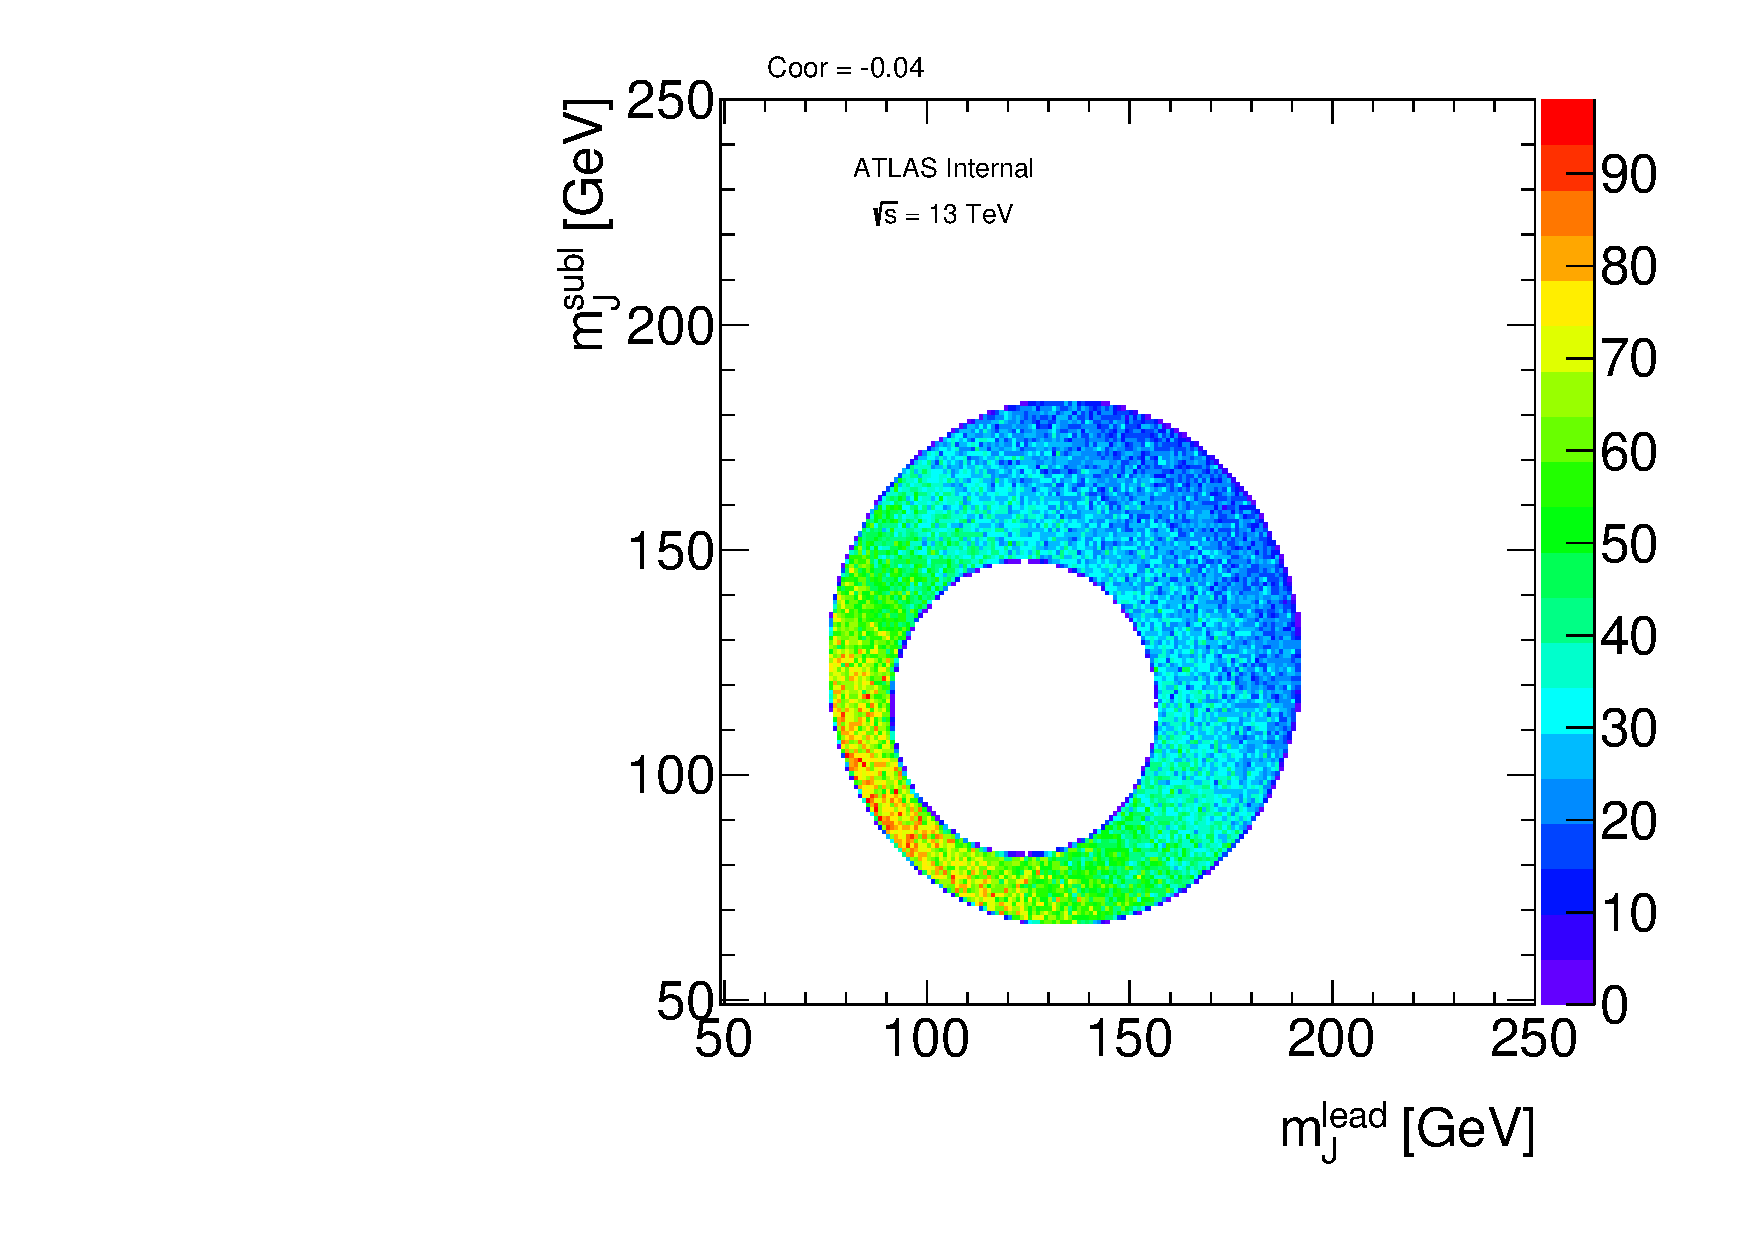
\includegraphics[angle=270, width=0.45\textwidth]{./figures/boosted/Other/Sideband_OneTag_mH0H1.pdf}
  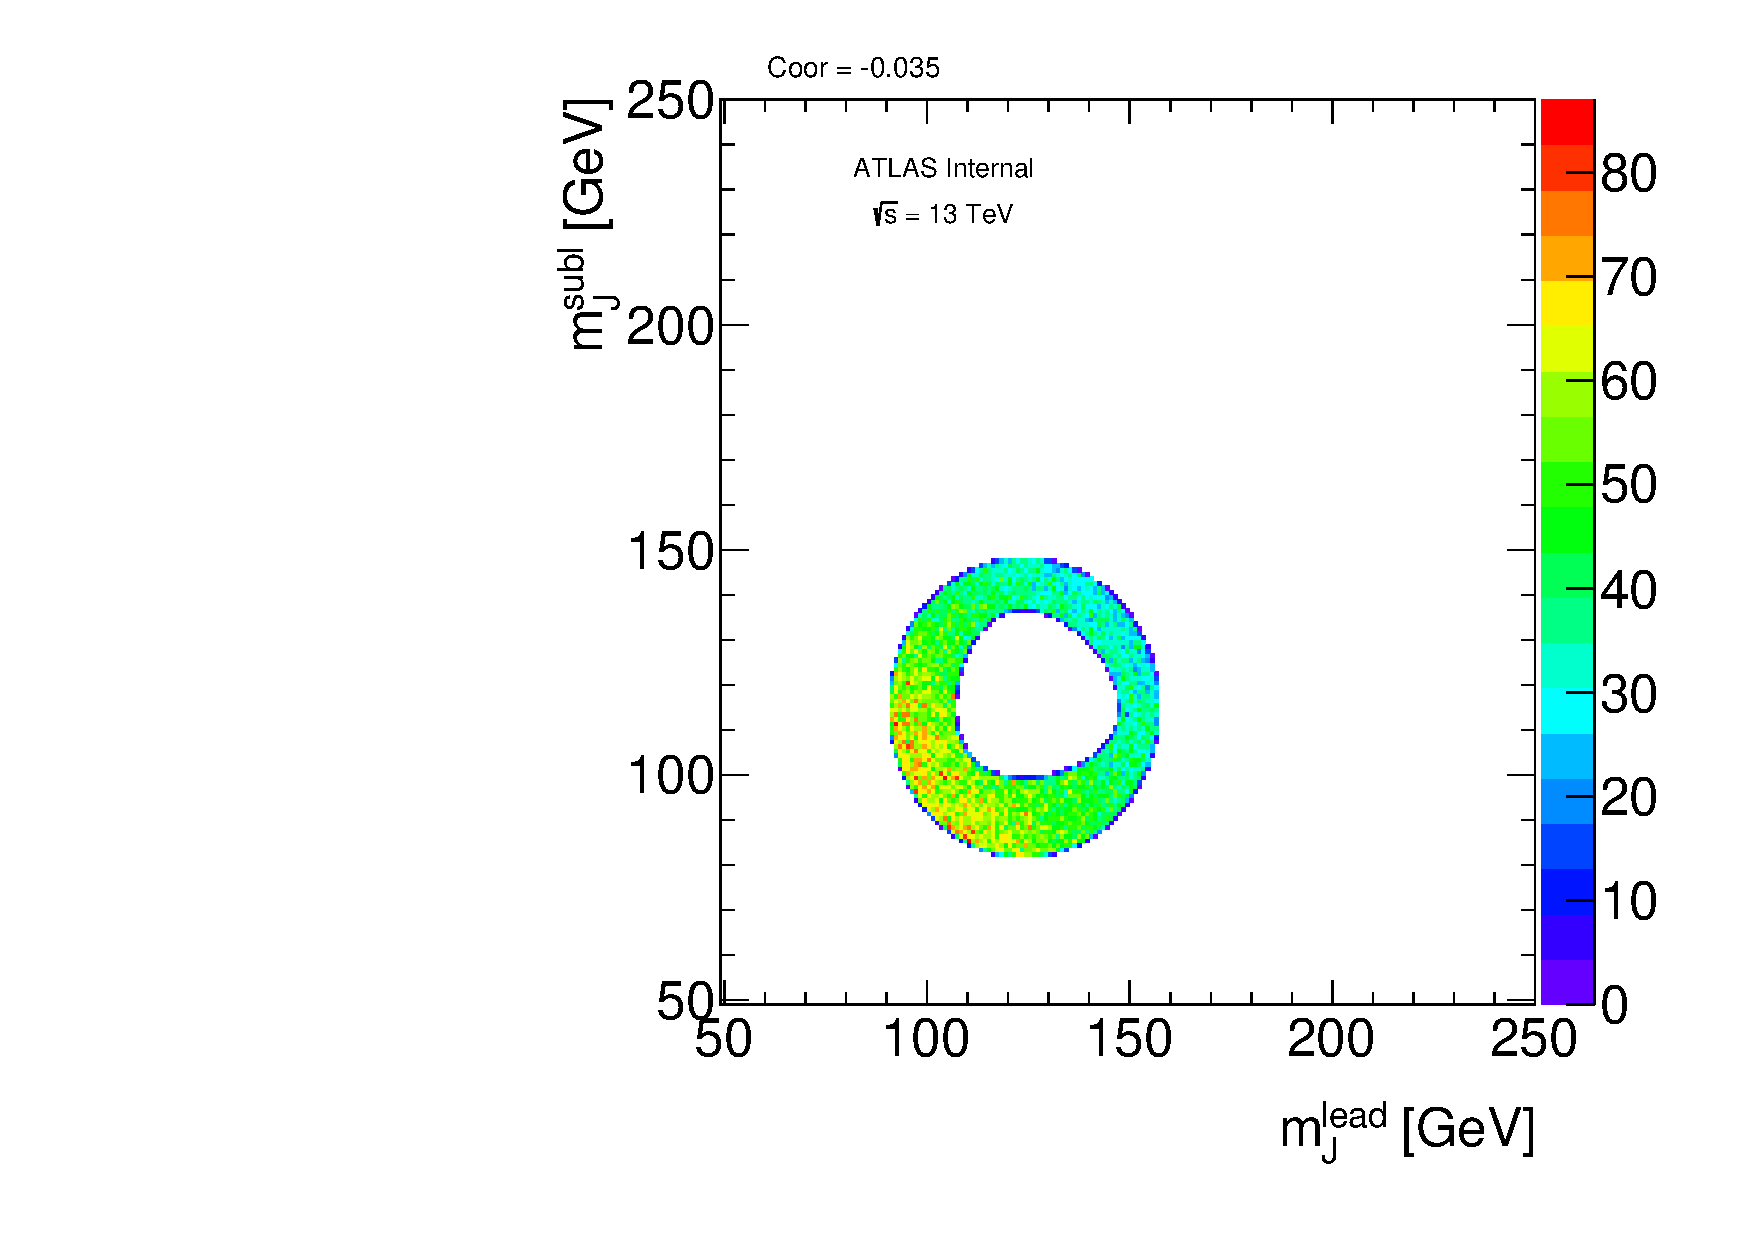
\includegraphics[angle=270, width=0.45\textwidth]{./figures/boosted/Other/Control_OneTag_mH0H1.pdf}\\
  \includegraphics[angle=270, width=0.45\textwidth]{./figures/boosted/Other/Sideband_TwoTag_mH0H1.pdf}
  \includegraphics[angle=270, width=0.45\textwidth]{./figures/boosted/Other/Control_TwoTag_mH0H1.pdf}
  \caption{$m_J^{lead}$ vs. $m_J^{subl}$ in data in the 1$b$-tag (top) and 2$b$-tag (bottom) selection, the plots show the boundary between the Sideband (left) and Control (right) regions.}
  \label{fig:boosted-region-def}
\end{center}
\end{figure*}

\paragraph{}
The CR is chosen to be as close as possible to the signal region, thus allows a good test for the background predictions, avoids the top mass peak around 175 GeV, and still gives reasonably statistics.  The SB definition is optimized so as to also be a reasonable proxy for the events contained in the CR and SR. Being farther from the SR means that the exact kinematics will not be the same, but one can avoid very large and very small mass jets not present in the SR by appropriate choice of SB.   The optimization of teh CR and SB definitiona can be found in Appendix~\ref{app:SB-optimization}. The choice of SB's impact on the predicted QCD background normalization, which is derived from the SB, can be found in Appendix~\ref{app:muqcd-study}.


\pagebreak{}
\subsection{QCD multi-jets}
\label{sec:boosted-qcd}

\paragraph{}
The QCD multi-jets prediction relies on finding a region which is similar enough in event properties so that it can be used to estimate the shapes of the expected background. This region is defined to be identical to the signal region except requiring both of the large-$R$ jets to pass the $\geq 2$( like in $4b$) or $\geq 1/2$ (like in $3b$) or $\geq 1$(like in $2b$ split) track jet requirement, but have two or one associated $b$-tagged track jets only on one of the large-$R$ jets. However, this $1b/2b$ region only provides shapes of the expected background and not the total yield. 

\paragraph{}
It should be noted that the $1b/2b$ region is orthogonal to the $4b/3b/2bs$ signal regions. In addition, the MC predicted $t\bar{t}$ events in the $1b/2b$ regions are subtracted from the data to produce the $1b/2b$ QCD estimation. This procedure follows closely the method used in Run 1 and also used in the resolved analysis, but requiring $1b$-tag for the $2bs$ background estimation.

\label{par:boosted-qcd-2bseperate}
\paragraph{} It should also be noted that the $2b$ sample is further split into $80\%-20\%$ parts, where each is used separately for 3$b$ and 4$b$ background estimations. This ensures the shape estimations of 3$b$ and 4$b$ QCD estimates are uncorrelated. 

It should also be noted that the resolved veto will impact the 4$b$ background estimation.  Specifically, 2$b$ events are excluded when they have at least two resolved jets that are $b$ tagged (passing resolved $70\%$ working point) and passing the resolved $Xhh < 1.6$ cut if using two other non b-tagged resolved jets to make the Higgs candidates. This ensures that a similar sculpting effect is reflected in the background estimation, and a check for this can be found in Appendix ~\ref{app:resveto}.

Given the $1b/2b$ samples, which predict shapes for the QCD background, the normalization of the QCD background is determined in the sideband by fitting the leading jet mass distribution simultaneously with QCD and $t\bar{t}$ background templates, as described in section~\ref{sec:ttbarnorm}.  This fit gives a scaling factor for QCD, called $\mu_{QCD}$ (and for $t\bar{t}$, called $\alpha_{t\bar{t}}$) which can be applied to scale the $1b/2b$ predictions in the CR or SR to the predicted normalizations in those regions.

It should be noted that there can be kinematic differences between the  $1b/2b$ samples and the $4b/3b/2bs$ regions.  Thus a kinematic reweighting is applied to correct for such differences, as described in Section~\ref{sec:boosted-reweight}.


%\paragraph{} 
%This background estimation is contingent on the idea that the 0$b$ sample QCD shape is a good estimate of $4/3/2bs$ samples QCD shapes. In addition, the use %of the SB region to estimate the background normalization relies on the SB to also accurately describe the normalization in the CR and SR regions.  The %purpose of the CR is thus to test both of these hypotheses. 

%\paragraph{} 
%While the normalizations of the $4b/3b/2bs$ split QCD predictions will be different, as they use events in the respective $4b$, $3b$, $2bs$ SB regions to set the normalizations, the shape estimates for the $4b/3b/2bs$  QCD predictions will be similar as they are both derived from the $1b/2b$ sample but only differ based on the number of $b$-tagged track jets required in each \largeR\ jet.



%As a final note, as discussed in Appendix~\ref{app:boosted_signal_migration}, we want to avoid possible signal contamination in the $2b$ regions used in our QCD predictions.  The primary concern for this contamination is in the SR prediction at high mass, where the expected backgrounds are small.  As such, in the $2b$ sample in the SR, we do not use (or look at) events above 2 TeV.  For background predictions above 2 TeV, we will perform a background smoothing up to 2 TeV using an exponential function, and will extrapolate above 2 TeV (see Section~\ref{sec:boosted-SR-smoothing}).  The choice of 2 TeV as a transition point was determined by ensuring that the signal contamination in dijet mass regions was at the few percent level or less (even when scaling by expected signal strength limits), as described in more detail in  Section~\ref{sec:boosted-SR-smoothing}.


%%%%%%%%%%%%%%%%%%%%%%%%%%%%%%%%%%%%%%%%%%%%%%%%%%%%%%%%%%%%%%%%%%%%%%%
%%%%%%%%%%%%%%%%%%%%%%%%%%%%%%%%%%%%%%%%%%%%%%%%%%%%%%%%%%%%%%%%%%%%%%%
%%%  SB. CR
%%%%%%%%%%%%%%%%%%%%%%%%%%%%%%%%%%%%%%%%%%%%%%%%%%%%%%%%%%%%%%%%%%%%%%%
%%%%%%%%%%%%%%%%%%%%%%%%%%%%%%%%%%%%%%%%%%%%%%%%%%%%%%%%%%%%%%%%%%%%%%%



\pagebreak{}
\subsection{\ttbar background}
\label{sec:boosted-ttbar}

\paragraph{}
The number of \ttbar\ events in the signal region coming mainly from the all-hadronic decay mode (with a smaller contribution from the leptonic + jets decay mode) comprises of  around 5-20\%  of the inclusive total background in the $4b/3b/2bs$ regions due to the high \pt\ threshold imposed on the leading \largeR calorimeter jet. In addition, the normalization and the shape of \ttbar\ events in the sideband region can affect the QCD estimate described in the previous section.

\paragraph{}
For the normalization of the $t\bar{t}$ background, we start with the MC prediction estimated by scaling the MC sample by the cross section and luminosity, and then applying the boosted event selection.  To account for possible differences between data and MC, a normalization scaling factor  is derived from a fit to data in the sideband region.  Although estimated in the SB, this normalization scaling factor will be applied also in the CR and SR.  Separate fits are done in the $4b/3b/2bs$  SB, thus deriving separate normalization scaling factor for the $4b/3b/2bs$ samples. For the shape of the $t\bar{t}$ background, no data driven methods were identified, and thus the MC shape is used.  

\paragraph{}
However, it should be noted that in the $4b$ and $3b$ signal region, there were not sufficient MC statistics to get a reasonable shape estimate.  As a result, in the $4b$ and $3b$ signal region,  the $2bs$ shapes will be used (but the normalization will still be that estimated for the $4b$/$3b$ sample). Since the same shape is used for the $4b/3b/2bs$ SR predictions of $t\bar{t}$, the shape systematics are considered correlated in the final results and limit setting. A comparison between the $4b/3b/2bs$ shapes for the di-large-$R$-jet mass distributions (the final discriminant) in the SR can be found in Figure~\ref{fig:ttshapeComp}.  As we can see, the shapes are compatible, with the $4b$ having much larger statistical uncertainties.  Differences between these distributions will be used as a systematic, as described in Section~\ref{sec:systematics}.

\begin{figure}[htbp!]
\begin{center}
  \includegraphics[angle=270, width=0.5\textwidth]{figures/boosted/Other/ttbar_compare_mHH_l.pdf}
\caption{comparison between the $2b$, $3b$, and $4b$ shapes for the di-large-$R$-jet mass distributions (the final discriminant) in the SR.}
\label{fig:ttshapeComp}
\end{center}
\end{figure}

%%%%%%%%%%%%%%%%%%%%%%%%%%%%%%%%%%%%%%%%%%%%%%%%%%%%%%%%%%%%%%%%%%%%%%%
%%%%%%%%%%%%%%%%%%%%%%%%%%%%%%%%%%%%%%%%%%%%%%%%%%%%%%%%%%%%%%%%%%%%%%%
%%%  Fitting
%%%%%%%%%%%%%%%%%%%%%%%%%%%%%%%%%%%%%%%%%%%%%%%%%%%%%%%%%%%%%%%%%%%%%%%
%%%%%%%%%%%%%%%%%%%%%%%%%%%%%%%%%%%%%%%%%%%%%%%%%%%%%%%%%%%%%%%%%%%%%%%

\pagebreak{}
\subsection{Fitting procedure for QCD and \ttbar\ normalization}
\label{sec:ttbarnorm}

\paragraph{}
The number of 4$b$/3$b$/2$b$s events in data observed in a given region (SB / CR / SR) can be described as:
\begin{eqnarray}\label{eq:fitparams}
N^{\nu_b}_{\text{data}} = \mu_{\text{qcd}}^{\nu_b} N^{xb}_{\text{qcd}} + \alpha_{t\bar{t}}^{\nu_b} N^{\nu_b}_{t\bar{t}} + N^{\nu_b}_{Z+jets}
\end{eqnarray}
where $\nu_b$ is the number of $b$-tagged track jets required, x is 1 for 2$b$s and 2 for 3$b$ and 4$b$. \muqcd\ is essentially an estimate of the ratio of the number of  QCD events with $\nu_b$ $b$-tagged track jets, to the number of $1b/2b$ QCD events, while the \ttbar\ normalization parameter $\alpha_{t\bar{t}}$\, applied after the \ttbar\ is scaled to the total integrated luminosity, is a correction to the MC prediction in this phase space. The same equation can be applied to the 4$b$/3$b$/2$b$s region (replacing $\nu_b$ by 4b/3b/2s $b$ in Equation~\ref{eq:fitparams}).   

\paragraph{}
In order to constrain the QCD and \ttbar\ background normalizations using data, a simultaneous fit is applied to extract both the \ttbar\ normalization with respect to the yields from simulation and the number of $1b/2b$ data events for the QCD background.  These scaling parameters are determined independently for the $4b/3b/2s$ signal regions. But as the procedure is the same for those three signal regions, we denote these scaling factors simply \muqcd and $\alpha_{t\bar{t}}$ in the following text.

\paragraph{}
A binned maximum likelihood fit is employed to find the values of \muqcd and $\alpha_{t\bar{t}}$, as well as the correlation between the two parameters. The fit is performed on the leading-\pt\ jet mass spectrum in the sideband region, as it has the best separation between QCD and \ttbar\ shapes. Due to the \pt$>450$ GeV cut imposed on the leading \largeR jet, the hadronic top quark is likely to be fully reconstructed inside of the \largeR jet and the leading jet mass in the \ttbar\ sample has a clean peak around $M=170$ GeV in the sideband region.

\paragraph{}
The values of \muqcd and $\alpha_{t\bar{t}}$ as estimated by the fits in the $4b/3b/2bs$ sideband regions can be found in Table~\ref{tab:bkgfit}, along with the correlation of the fitted parameters $\rho(\mu_{qcd},\alpha_{t\bar{t}}) = \frac{Cov(\mu_{qcd},\ \alpha_{t\bar{t}})}{\sigma_{\mu_{qcd}}\sigma_{\alpha_{t\bar{t}}} }$. \muqcd and $\alpha_{t\bar{t}}$ are approximately 70\% negatively correlated, which is not surprising as they are the only two components fit to the data distribution and their sum needs to predict the SB total event count.

\begin{table}[htbp!]
\begin{center}
\begin{footnotesize} 
\begin{tabular}{c|c|c|c} 
Sample & $\mu_{qcd}$ & $\alpha_{t\bar{t}}$ & $\rho(\mu_{qcd}, \alpha_{t\bar{t}})$ \\ 
\hline\hline 
FourTag & 0.033167 $\pm$ 0.0042799 & 0.89136 $\pm$ 0.59866 & -0.7846\\
ThreeTag & 0.16256 $\pm$ 0.0043405 & 0.79989 $\pm$ 0.073276 & -0.72029\\
TwoTag split & 0.062726 $\pm$ 0.00057307 & 0.98637 $\pm$ 0.018582 & -0.4698\\
\hline\hline 
\end{tabular} 
\end{footnotesize} 
\newline 

\caption{Background scaling parameters (\muqcd and $\alpha_{t\bar{t}}$) estimated from fits to the leading jet mass distributions in $4b/3b/2bs$ sideband regions. $\rho(\mu_{qcd},\alpha_{t\bar{t}}) = \frac{Cov(\mu_{qcd},\ \alpha_{t\bar{t}})}{\sigma_{\mu_{qcd}}\sigma_{\alpha_{t\bar{t}}} }$}
\label{tab:bkgfit}
\end{center}
\end{table}

\paragraph{}
Figure~\ref{fig:ttbar-fit} shows the post-fit spectrum of the leading \largeR calorimeter jet mass in the 4$b$/3$b$/2$b$s sideband regions. The normalization of \ttbar\ is 
constrained by the top quark mass peak around 170~GeV. The shapes of the data is also well modeled by the predicted background. The fitting errors on \muqcd and 
$\alpha_{t\bar{t}}$ are applied as systematic uncertainties taking into account their correlation. This will be explained in more detail in the systematics section.

\begin{figure}[htbp!]
\begin{center}
 \includegraphics[angle=270, width=0.45\textwidth]{./figures/boosted/Fit/fitNorm_i4.pdf}\\
 \includegraphics[angle=270, width=0.45\textwidth]{./figures/boosted/Fit/fitNorm_i3.pdf}\\
 \includegraphics[angle=270, width=0.45\textwidth]{./figures/boosted/Fit/fitNorm_i2s.pdf}\\
\caption{Simultaneous fit of \muqcd and \alphatt in 4$b$ (top) and 3$b$ (middle) and $2b$ (bottom) sideband region using leading \largeR calorimeter jet mass spectrum.}
\label{fig:ttbar-fit}
\end{center}
\end{figure}

\clearpage

%%%%%%%%%%%%%%%%%%%%%%%%%%%%%%%%%%%%%%%%%%%%%%%%%%%%%%%%%%%%%%%%%%%%%%%
%%%%%%%%%%%%%%%%%%%%%%%%%%%%%%%%%%%%%%%%%%%%%%%%%%%%%%%%%%%%%%%%%%%%%%%
%%%  Reweighting
%%%%%%%%%%%%%%%%%%%%%%%%%%%%%%%%%%%%%%%%%%%%%%%%%%%%%%%%%%%%%%%%%%%%%%%
%%%%%%%%%%%%%%%%%%%%%%%%%%%%%%%%%%%%%%%%%%%%%%%%%%%%%%%%%%%%%%%%%%%%%%%

\subsection{Kinematic reweighting}
\label{sec:boosted-reweight}
%%\paragraph{}
Due to the large contribution from the completely data-driven QCD background, it is important to model this background as good as possible in all regions of the analysis. Using the $1/2b$ region to model the 2$b$s, 3$b$, and 4$b$ regions can introduce discrepancies in the modeling of the estimated QCD background versus the real n$b$ data. These discrepancies arise possibly from the non-trivial effect that $b$-tagging has on jet kinematics. The natural choice of reweighting variable is the $p_{T}$ of the track jets in the event, since these are the objects that we apply the $b$-tagging to. Also, large-$R$ jet $p_{T}$ is also reweighted to account for the effect from light and charm quark composition difference at different energy scales. The three chosen variables are the leading large-$R$ jet $p_{T}$, leading large-$R$ jet leading trackjet $p_{T}$ and subleading large-$R$ jet leading trackjet $p_{T}$.

%%\paragraph{}
In order to account for the $b$-tagging effect, a reweighting on the $1/2b$ data is adopted. The basic idea is to reweight the non $b$-tagged Higgs candidate to have kinematic distributions just like a $b$-tagged Higgs candidate. The idea is demonstrated in Figure~\ref{fig:rw-2bs-comp}. It shows that 2$b$s has very similar kinematic distributions on the trackjet \pt as the 1$b$ sample, when the variable is the $b$ tagged trackjet. 

%%\paragraph{}
For 2$b$s, the 1$b$ non-tagged Higgs candidate is reweighted to be like a 1$b$ tagged Higgs candiate; for 3$b$, the 2$b$ non-tagged Higgs candidate is reweighted to be like a 1$b$ tagged Higgs candidate; for 4$b$, the 2$b$ non-tagged Higgs candidate is reweighted to be like a 2$b$ tagged Higgs candidate. For each category, the events are split into two orthogonal subgroups, depending on whether leading/subleading Higgs candidate is $b$-tagged, the event is then reweighted such that the untagged Higgs candidate's distribution behaves like the corresponding $b$-tagged Higgs candidate's.

%%%%%%%%%%%%%%%%%%%%%%%%%%%
\begin{figure*}[htbp!]
\begin{center}
\includegraphics[width=0.4\textwidth,angle=-90]{figures/boosted/Prereweight/2bs_directcompare_leadHCand_trk0_Pt_1.pdf}
\includegraphics[width=0.4\textwidth,angle=-90]{figures/boosted/Prereweight/2bs_directcompare_leadHCand_trk1_Pt_1.pdf}\\
\includegraphics[width=0.4\textwidth,angle=-90]{figures/boosted/Prereweight/2bs_directcompare_sublHCand_trk0_Pt_1.pdf}
\includegraphics[width=0.4\textwidth,angle=-90]{figures/boosted/Prereweight/2bs_directcompare_sublHCand_trk1_Pt_1.pdf}\\
\caption{Comparison of different trackjet \pt distributions. Top row is for leading \pt Higgs candidate, and bottom row is for subleading \pt Higgs candidate. Left column is for the leading \pt trackjet of the Higgs candidate, and right column is for the subleading \pt trackjet of the Higgs candidate. Shown in the plot are just data distributions, inclusive of SB, CR, and SR regions for 0$b$ and 1$b$, while for 2$b$s only the SB region is shown. 1$b$ sample is further split into four subcategories, depending on which trackjet gets $b$ tagged. OneTag lead on lead means the $b$ tagged trackjet is the leading trackjet of the leading Higgs candidate, OneTag lead on subl means the $b$ tagged trackjet is the subleading trackjet of the leading Higgs candidate, OneTag subl on lead means the $b$ tagged trackjet is the leading trackjet of the subleading Higgs candidate, and OneTag subl on subl means the $b$ tagged trackjet is the subleading trackjet of the subleading Higgs candidate. At the bottom ratio plot, all the ratio are taken with respect to the 0$b$ tagged distribution.}
\label{fig:rw-2bs-comp}
\end{center}
\end{figure*}

%%\paragraph{}
To avoid potential biases in the final distributions used for the analysis, a reweighting technique is applied to the $1/2b$ data only. Since each signal region is modeled by a different $1/2b$ tag category: 2$b$s by 1$b$ tag events with at least 1 track jets on both large-$R$ jets, 3$b$ by 2$b$ tag events with at least one track jets on one large-$R$ jet and at least two track jets on the other large-$R$ jet, and 4$b$ by 2$b$ tag events with at least two track jets on both large-$R$ jets, the reweighting procedure is the same but orthogonal for the three different channels. Note the 2$b$ sample is already split into seperate parts, as described in paragraph \ref{par:boosted-qcd-2bseperate}.

\clearpage{}
%%\paragraph{}
The detailed procedure is listed as follows:
\begin{itemize}
\item Substracting $1/2b$ tag $t\bar{t}$ and $Z+$jets samples in the sideband from the $1/2b$ tag data in the Sideband + Control + Signal regions to get the $1/2b$ QCD inclusive estimate.
\item Seperate the $1/2b$ tag sample further to sample: A. that has the $b$-tagged Higgs is the leading \pt Higgs candidate, and B. that the $b$-tagged Higgs is the subleading \pt Higgs candidate.
\item For each variable, i.e. the large-$R$ jet $p_{T}$, normalize sample A to sample B total number of events, take the ratio of sample A distribution over sample B distribution, and fit the ratio with a spline function. (TSpline3)
\item Use this functional form to extract reweighting values for each variable that is considered. The reweighting value for each variable is also constrained to be within a $-30\%$ to $+40\%$ range compared to one, to avoid over corrections and failed fit situations. 
%Then, the difference from one is scaled by $0.618$ (the golden ratio) to get a new weight, which is applied later. This accounts for over correlation by the spline and accerlerates convergence.
\item For each event, all the weights are multiplied together to change the $1/2b$ tag data event weight. Another constraint is applied, such that each total reweighting value is constrained to be within a $10\%$ to $+1000\%$ range compared to one, again to avoid over corrections.
\item The reweighting is done on the three variables: large-$R$ jet $p_{T}$ and the two track jet $p_{T}$s, which is counted as one iteration of reweighting.
\item A total of ten iterations are used to stabalize the reweighting. The reweighting is roughly converging after three iterations.
\end{itemize}

%%\paragraph{}
For reweighting method comparisons and validations in data and Dijet MC, see Appendix~\ref{app:reweightstudy}.

\subsubsection{Reweighting Fits}
\label{sec:boosted-Reweight-Fit}
%%\paragraph{}
The first iteration, second iteration, and last iteration of fits for 2$b$s, where in 1$b$ data, the non-tagged Higgs candidate are reweighted to be like a 1$b$ tagged Higgs candidate, can be seen in Figure~\ref{fig:rw-2bs-lead} and ~\ref{fig:rw-2bs-subl}. Similar distributions for 3$b$, where in 2$b$ data, the non-tagged Higgs candidate are reweighted to be like a 1$b$ tagged Higgs candidate, are shown in Figure~\ref{fig:rw-3b-lead} and ~\ref{fig:rw-3b-subl}. Similar distributions for 4$b$, where in 2$b$ data, the non-tagged Higgs candidate are reweighted to be like a 2$b$ tagged Higgs candidate, are shown in Figure~\ref{fig:rw-4b-lead} and ~\ref{fig:rw-4b-subl}. The before reweighting distribution (first row), the reweighting result after the first interation (second row), and the final distribution after reweighting (last row) are presented.

%%\paragraph{}
It should be noted that in the some plots, like Figure~\ref{fig:rw-4b-lead} and ~\ref{fig:rw-4b-subl}, the last ratio bin sometimes still doesn't converge to unity. This is a feature from the limited statistics from the last bin, especially in the 4$b$ case, where only $20\%$ number of events in 2$b$ is used for background prediction and therefore reweighted. One could choose a different binning and use more iterations to help this converge to one, yet the last bin's few event will also likely to end up with a large unphysical weight and therefore harm the background prediction later.

%%\paragraph{}
For the distribution of weights and the weight as a function of different kinematic ranges, see Appendix~\ref{app:reweight-dist}.
%%%%%%%%%%%%%%%%%%%%%%%%%%% original distributions
\begin{figure*}[htbp!]
\begin{center}
\includegraphics[width=0.32\textwidth,angle=-90]{figures/boosted/Reweight/Fits/Moriond_NoTag_2Trk_split_lead_Incl_sublHCand_Pt_m_1.pdf}
\includegraphics[width=0.32\textwidth,angle=-90]{figures/boosted/Reweight/Fits/Moriond_NoTag_2Trk_split_lead_Incl_sublHCand_trk0_Pt.pdf}
\includegraphics[width=0.32\textwidth,angle=-90]{figures/boosted/Reweight/Fits/Moriond_NoTag_2Trk_split_lead_Incl_sublHCand_trk1_Pt.pdf} \\
\includegraphics[width=0.32\textwidth,angle=-90]{figures/boosted/Reweight/Fits/Moriond_bkg_0_NoTag_2Trk_split_lead_Incl_sublHCand_Pt_m_1.pdf}
\includegraphics[width=0.32\textwidth,angle=-90]{figures/boosted/Reweight/Fits/Moriond_bkg_0_NoTag_2Trk_split_lead_Incl_sublHCand_trk0_Pt.pdf}
\includegraphics[width=0.32\textwidth,angle=-90]{figures/boosted/Reweight/Fits/Moriond_bkg_0_NoTag_2Trk_split_lead_Incl_sublHCand_trk1_Pt.pdf} \\
\includegraphics[width=0.32\textwidth,angle=-90]{figures/boosted/Reweight/Fits/Moriond_bkg_3_NoTag_2Trk_split_lead_Incl_sublHCand_Pt_m_1.pdf}
\includegraphics[width=0.32\textwidth,angle=-90]{figures/boosted/Reweight/Fits/Moriond_bkg_3_NoTag_2Trk_split_lead_Incl_sublHCand_trk0_Pt.pdf}
\includegraphics[width=0.32\textwidth,angle=-90]{figures/boosted/Reweight/Fits/Moriond_bkg_3_NoTag_2Trk_split_lead_Incl_sublHCand_trk1_Pt.pdf} \\
\includegraphics[width=0.32\textwidth,angle=-90]{figures/boosted/Reweight/Fits/Moriond_bkg_9_NoTag_2Trk_split_lead_Incl_sublHCand_Pt_m_1.pdf}
\includegraphics[width=0.32\textwidth,angle=-90]{figures/boosted/Reweight/Fits/Moriond_bkg_9_NoTag_2Trk_split_lead_Incl_sublHCand_trk0_Pt.pdf}
\includegraphics[width=0.32\textwidth,angle=-90]{figures/boosted/Reweight/Fits/Moriond_bkg_9_NoTag_2Trk_split_lead_Incl_sublHCand_trk1_Pt.pdf} \\
\caption{For $2b$s background estimate: the fits to the ratio of the data in the 1$b$ category, of the sublleading Higgs candidate 1$b$-tagged events's subleading Higgs candidate distributions(black point), over the leading Higgs candidate 1$b$-tagged events's subleading Higgs candidate distributions(yellow). Distributions and fits to the estimated QCD background for large-$R$ jet $p_{T}$ (left),  the large-$R$ jet's leading trackjet $p_T$ (middle), and large-$R$ jet's subleading trackjet $p_T$ (right) are shown.  Figure are shown before reweighting (top row), after the first iteration(second row), after the fourth iteration(third row), and after the last iteration (bottow row). The green line is the spline extrapolation; and the red line is a polynomial fit.}
\label{fig:rw-2bs-lead}
\end{center}
\end{figure*}

\begin{figure*}[htbp!]
\begin{center}
\includegraphics[width=0.32\textwidth,angle=-90]{figures/boosted/Reweight/Fits/Moriond_NoTag_2Trk_split_subl_Incl_leadHCand_Pt_m_1.pdf}
\includegraphics[width=0.32\textwidth,angle=-90]{figures/boosted/Reweight/Fits/Moriond_NoTag_2Trk_split_subl_Incl_leadHCand_trk0_Pt.pdf}
\includegraphics[width=0.32\textwidth,angle=-90]{figures/boosted/Reweight/Fits/Moriond_NoTag_2Trk_split_subl_Incl_leadHCand_trk1_Pt.pdf} \\
\includegraphics[width=0.32\textwidth,angle=-90]{figures/boosted/Reweight/Fits/Moriond_bkg_0_NoTag_2Trk_split_subl_Incl_leadHCand_Pt_m_1.pdf}
\includegraphics[width=0.32\textwidth,angle=-90]{figures/boosted/Reweight/Fits/Moriond_bkg_0_NoTag_2Trk_split_subl_Incl_leadHCand_trk0_Pt.pdf}
\includegraphics[width=0.32\textwidth,angle=-90]{figures/boosted/Reweight/Fits/Moriond_bkg_0_NoTag_2Trk_split_subl_Incl_leadHCand_trk1_Pt.pdf} \\
\includegraphics[width=0.32\textwidth,angle=-90]{figures/boosted/Reweight/Fits/Moriond_bkg_3_NoTag_2Trk_split_subl_Incl_leadHCand_Pt_m_1.pdf}
\includegraphics[width=0.32\textwidth,angle=-90]{figures/boosted/Reweight/Fits/Moriond_bkg_3_NoTag_2Trk_split_subl_Incl_leadHCand_trk0_Pt.pdf}
\includegraphics[width=0.32\textwidth,angle=-90]{figures/boosted/Reweight/Fits/Moriond_bkg_3_NoTag_2Trk_split_subl_Incl_leadHCand_trk1_Pt.pdf} \\
\includegraphics[width=0.32\textwidth,angle=-90]{figures/boosted/Reweight/Fits/Moriond_bkg_9_NoTag_2Trk_split_subl_Incl_leadHCand_Pt_m_1.pdf}
\includegraphics[width=0.32\textwidth,angle=-90]{figures/boosted/Reweight/Fits/Moriond_bkg_9_NoTag_2Trk_split_subl_Incl_leadHCand_trk0_Pt.pdf}
\includegraphics[width=0.32\textwidth,angle=-90]{figures/boosted/Reweight/Fits/Moriond_bkg_9_NoTag_2Trk_split_subl_Incl_leadHCand_trk1_Pt.pdf} \\
\caption{For $2b$s background estimate: the fits to the ratio of the data in the 1$b$ category, of the leading Higgs candidate 1$b$-tagged events's leading Higgs candidate distributions(black point), over the sublleading Higgs candidate 1$b$-tagged events's leading Higgs candidate distributions(yellow). Distributions and fits to the estimated QCD background for large-$R$ jet $p_{T}$ (left),  the large-$R$ jet's leading trackjet $p_T$ (middle), and large-$R$ jet's subleading trackjet $p_T$ (right) are shown.  Figure are shown before reweighting (top row), after the first iteration(second row), after the fourth iteration(third row), and after the last iteration (bottow row). The green line is the spline extrapolation; and the red line is a polynomial fit.}
\label{fig:rw-2bs-subl}
\end{center}
\end{figure*}

\begin{figure*}[htbp!]
\begin{center}
\includegraphics[width=0.32\textwidth,angle=-90]{figures/boosted/Reweight/Fits/Moriond_NoTag_3Trk_lead_Incl_sublHCand_Pt_m_1.pdf}
\includegraphics[width=0.32\textwidth,angle=-90]{figures/boosted/Reweight/Fits/Moriond_NoTag_3Trk_lead_Incl_sublHCand_trk0_Pt.pdf}
\includegraphics[width=0.32\textwidth,angle=-90]{figures/boosted/Reweight/Fits/Moriond_NoTag_3Trk_lead_Incl_sublHCand_trk1_Pt.pdf} \\
\includegraphics[width=0.32\textwidth,angle=-90]{figures/boosted/Reweight/Fits/Moriond_bkg_0_NoTag_3Trk_lead_Incl_sublHCand_Pt_m_1.pdf}
\includegraphics[width=0.32\textwidth,angle=-90]{figures/boosted/Reweight/Fits/Moriond_bkg_0_NoTag_3Trk_lead_Incl_sublHCand_trk0_Pt.pdf}
\includegraphics[width=0.32\textwidth,angle=-90]{figures/boosted/Reweight/Fits/Moriond_bkg_0_NoTag_3Trk_lead_Incl_sublHCand_trk1_Pt.pdf} \\
\includegraphics[width=0.32\textwidth,angle=-90]{figures/boosted/Reweight/Fits/Moriond_bkg_3_NoTag_3Trk_lead_Incl_sublHCand_Pt_m_1.pdf}
\includegraphics[width=0.32\textwidth,angle=-90]{figures/boosted/Reweight/Fits/Moriond_bkg_3_NoTag_3Trk_lead_Incl_sublHCand_trk0_Pt.pdf}
\includegraphics[width=0.32\textwidth,angle=-90]{figures/boosted/Reweight/Fits/Moriond_bkg_3_NoTag_3Trk_lead_Incl_sublHCand_trk1_Pt.pdf} \\
\includegraphics[width=0.32\textwidth,angle=-90]{figures/boosted/Reweight/Fits/Moriond_bkg_9_NoTag_3Trk_lead_Incl_sublHCand_Pt_m_1.pdf}
\includegraphics[width=0.32\textwidth,angle=-90]{figures/boosted/Reweight/Fits/Moriond_bkg_9_NoTag_3Trk_lead_Incl_sublHCand_trk0_Pt.pdf}
\includegraphics[width=0.32\textwidth,angle=-90]{figures/boosted/Reweight/Fits/Moriond_bkg_9_NoTag_3Trk_lead_Incl_sublHCand_trk1_Pt.pdf} \\
\caption{For 3$b$ background estimate: the fits to the ratio of the data in the 2$b$ category, of the sublleading Higgs candidate 2$b$-tagged events's subleading Higgs candidate distributions(black point), over the leading Higgs candidate 1$b$-tagged events's subleading Higgs candidate distributions(yellow). Distributions and fits to the estimated QCD background for large-$R$ jet $p_{T}$ (left),  the large-$R$ jet's leading trackjet $p_T$ (middle), and large-$R$ jet's subleading trackjet $p_T$ (right) are shown.  Figure are shown before reweighting (top row), after the first iteration(second row), after the fourth iteration(third row), and after the last iteration (bottow row). The green line is the spline extrapolation; and the red line is a polynomial fit.}
\label{fig:rw-3b-lead}
\end{center}
\end{figure*}

\begin{figure*}[htbp!]
\begin{center}
\includegraphics[width=0.32\textwidth,angle=-90]{figures/boosted/Reweight/Fits/Moriond_NoTag_3Trk_subl_Incl_leadHCand_Pt_m_1.pdf}
\includegraphics[width=0.32\textwidth,angle=-90]{figures/boosted/Reweight/Fits/Moriond_NoTag_3Trk_subl_Incl_leadHCand_trk0_Pt.pdf}
\includegraphics[width=0.32\textwidth,angle=-90]{figures/boosted/Reweight/Fits/Moriond_NoTag_3Trk_subl_Incl_leadHCand_trk1_Pt.pdf} \\
\includegraphics[width=0.32\textwidth,angle=-90]{figures/boosted/Reweight/Fits/Moriond_bkg_0_NoTag_3Trk_subl_Incl_leadHCand_Pt_m_1.pdf}
\includegraphics[width=0.32\textwidth,angle=-90]{figures/boosted/Reweight/Fits/Moriond_bkg_0_NoTag_3Trk_subl_Incl_leadHCand_trk0_Pt.pdf}
\includegraphics[width=0.32\textwidth,angle=-90]{figures/boosted/Reweight/Fits/Moriond_bkg_0_NoTag_3Trk_subl_Incl_leadHCand_trk1_Pt.pdf} \\
\includegraphics[width=0.32\textwidth,angle=-90]{figures/boosted/Reweight/Fits/Moriond_bkg_3_NoTag_3Trk_subl_Incl_leadHCand_Pt_m_1.pdf}
\includegraphics[width=0.32\textwidth,angle=-90]{figures/boosted/Reweight/Fits/Moriond_bkg_3_NoTag_3Trk_subl_Incl_leadHCand_trk0_Pt.pdf}
\includegraphics[width=0.32\textwidth,angle=-90]{figures/boosted/Reweight/Fits/Moriond_bkg_3_NoTag_3Trk_subl_Incl_leadHCand_trk1_Pt.pdf} \\
\includegraphics[width=0.32\textwidth,angle=-90]{figures/boosted/Reweight/Fits/Moriond_bkg_9_NoTag_3Trk_subl_Incl_leadHCand_Pt_m_1.pdf}
\includegraphics[width=0.32\textwidth,angle=-90]{figures/boosted/Reweight/Fits/Moriond_bkg_9_NoTag_3Trk_subl_Incl_leadHCand_trk0_Pt.pdf}
\includegraphics[width=0.32\textwidth,angle=-90]{figures/boosted/Reweight/Fits/Moriond_bkg_9_NoTag_3Trk_subl_Incl_leadHCand_trk1_Pt.pdf} \\
\caption{For 3$b$ background estimate: the fits to the ratio of the data in the 2$b$ category, of the leading Higgs candidate 2$b$-tagged events's leading Higgs candidate distributions(black point), over the sublleading Higgs candidate 1$b$-tagged events's leading Higgs candidate distributions(yellow). Distributions and fits to the estimated QCD background for large-$R$ jet $p_{T}$ (left),  the large-$R$ jet's leading trackjet $p_T$ (middle), and large-$R$ jet's subleading trackjet $p_T$ (right) are shown.  Figure are shown before reweighting (top row), after the first iteration(second row), after the fourth iteration(third row), and after the last iteration (bottow row). The green line is the spline extrapolation; and the red line is a polynomial fit.}
\label{fig:rw-3b-subl}
\end{center}
\end{figure*}

\begin{figure*}[htbp!]
\begin{center}
\includegraphics[width=0.32\textwidth,angle=-90]{figures/boosted/Reweight/Fits/Moriond_NoTag_4Trk_lead_Incl_sublHCand_Pt_m_1.pdf}
\includegraphics[width=0.32\textwidth,angle=-90]{figures/boosted/Reweight/Fits/Moriond_NoTag_4Trk_lead_Incl_sublHCand_trk0_Pt.pdf}
\includegraphics[width=0.32\textwidth,angle=-90]{figures/boosted/Reweight/Fits/Moriond_NoTag_4Trk_lead_Incl_sublHCand_trk1_Pt.pdf} \\
\includegraphics[width=0.32\textwidth,angle=-90]{figures/boosted/Reweight/Fits/Moriond_bkg_0_NoTag_4Trk_lead_Incl_sublHCand_Pt_m_1.pdf}
\includegraphics[width=0.32\textwidth,angle=-90]{figures/boosted/Reweight/Fits/Moriond_bkg_0_NoTag_4Trk_lead_Incl_sublHCand_trk0_Pt.pdf}
\includegraphics[width=0.32\textwidth,angle=-90]{figures/boosted/Reweight/Fits/Moriond_bkg_0_NoTag_4Trk_lead_Incl_sublHCand_trk1_Pt.pdf} \\
\includegraphics[width=0.32\textwidth,angle=-90]{figures/boosted/Reweight/Fits/Moriond_bkg_3_NoTag_4Trk_lead_Incl_sublHCand_Pt_m_1.pdf}
\includegraphics[width=0.32\textwidth,angle=-90]{figures/boosted/Reweight/Fits/Moriond_bkg_3_NoTag_4Trk_lead_Incl_sublHCand_trk0_Pt.pdf}
\includegraphics[width=0.32\textwidth,angle=-90]{figures/boosted/Reweight/Fits/Moriond_bkg_3_NoTag_4Trk_lead_Incl_sublHCand_trk1_Pt.pdf} \\
\includegraphics[width=0.32\textwidth,angle=-90]{figures/boosted/Reweight/Fits/Moriond_bkg_9_NoTag_4Trk_lead_Incl_sublHCand_Pt_m_1.pdf}
\includegraphics[width=0.32\textwidth,angle=-90]{figures/boosted/Reweight/Fits/Moriond_bkg_9_NoTag_4Trk_lead_Incl_sublHCand_trk0_Pt.pdf}
\includegraphics[width=0.32\textwidth,angle=-90]{figures/boosted/Reweight/Fits/Moriond_bkg_9_NoTag_4Trk_lead_Incl_sublHCand_trk1_Pt.pdf} \\
\caption{For 4$b$ background estimate: the fits to the ratio of the data in the 2$b$ category, of the sublleading Higgs candidate 2$b$-tagged events's subleading Higgs candidate distributions(black point), over the leading Higgs candidate 2$b$-tagged events's subleading Higgs candidate distributions(yellow). Distributions and fits to the estimated QCD background for large-$R$ jet $p_{T}$ (left),  the large-$R$ jet's leading trackjet $p_T$ (middle), and large-$R$ jet's subleading trackjet $p_T$ (right) are shown.  Figure are shown before reweighting (top row), after the first iteration(second row), after the fourth iteration(third row), and after the last iteration (bottow row). The green line is the spline extrapolation; and the red line is a polynomial fit.}
\label{fig:rw-4b-lead}
\end{center}
\end{figure*}

\begin{figure*}[htbp!]
\begin{center}
\includegraphics[width=0.32\textwidth,angle=-90]{figures/boosted/Reweight/Fits/Moriond_NoTag_4Trk_subl_Incl_leadHCand_Pt_m_1.pdf}
\includegraphics[width=0.32\textwidth,angle=-90]{figures/boosted/Reweight/Fits/Moriond_NoTag_4Trk_subl_Incl_leadHCand_trk0_Pt.pdf}
\includegraphics[width=0.32\textwidth,angle=-90]{figures/boosted/Reweight/Fits/Moriond_NoTag_4Trk_subl_Incl_leadHCand_trk1_Pt.pdf} \\
\includegraphics[width=0.32\textwidth,angle=-90]{figures/boosted/Reweight/Fits/Moriond_bkg_0_NoTag_4Trk_subl_Incl_leadHCand_Pt_m_1.pdf}
\includegraphics[width=0.32\textwidth,angle=-90]{figures/boosted/Reweight/Fits/Moriond_bkg_0_NoTag_4Trk_subl_Incl_leadHCand_trk0_Pt.pdf}
\includegraphics[width=0.32\textwidth,angle=-90]{figures/boosted/Reweight/Fits/Moriond_bkg_0_NoTag_4Trk_subl_Incl_leadHCand_trk1_Pt.pdf} \\
\includegraphics[width=0.32\textwidth,angle=-90]{figures/boosted/Reweight/Fits/Moriond_bkg_3_NoTag_4Trk_subl_Incl_leadHCand_Pt_m_1.pdf}
\includegraphics[width=0.32\textwidth,angle=-90]{figures/boosted/Reweight/Fits/Moriond_bkg_3_NoTag_4Trk_subl_Incl_leadHCand_trk0_Pt.pdf}
\includegraphics[width=0.32\textwidth,angle=-90]{figures/boosted/Reweight/Fits/Moriond_bkg_3_NoTag_4Trk_subl_Incl_leadHCand_trk1_Pt.pdf} \\
\includegraphics[width=0.32\textwidth,angle=-90]{figures/boosted/Reweight/Fits/Moriond_bkg_9_NoTag_4Trk_subl_Incl_leadHCand_Pt_m_1.pdf}
\includegraphics[width=0.32\textwidth,angle=-90]{figures/boosted/Reweight/Fits/Moriond_bkg_9_NoTag_4Trk_subl_Incl_leadHCand_trk0_Pt.pdf}
\includegraphics[width=0.32\textwidth,angle=-90]{figures/boosted/Reweight/Fits/Moriond_bkg_9_NoTag_4Trk_subl_Incl_leadHCand_trk1_Pt.pdf} \\
\caption{For 4$b$ background estimate: the fits to the ratio of the data in the 2$b$ category, of the leading Higgs candidate 2$b$-tagged events's leading Higgs candidate distributions(black point), over the sublleading Higgs candidate 2$b$-tagged events's leading Higgs candidate distributions(yellow). Distributions and fits to the estimated QCD background for large-$R$ jet $p_{T}$ (left),  the large-$R$ jet's leading trackjet $p_T$ (middle), and large-$R$ jet's subleading trackjet $p_T$ (right) are shown.  Figure are shown before reweighting (top row), after the first iteration(second row), after the fourth iteration(third row), and after the last iteration (bottow row). The green line is the spline extrapolation; and the red line is a polynomial fit.}
\label{fig:rw-4b-subl}
\end{center}
\end{figure*}


\pagebreak{}
%%%%%%%%%%%%%%%%%%%%%%%%%%%
\subsubsection{Reweighting Results Comparison in Sideband and Control Region}
\label{sec:boosted-Reweight-compare}

%%\paragraph{}
A comparison of the Sideband shapes before and after reweighting for 2$b$s, 3$b$ and 4$b$ can be seen in Figures~\ref{fig:rw-2bs-comp-sb},~\ref{fig:rw-3b-comp-sb}, and ~\ref{fig:rw-4b-comp-sb}. Also, a comparison of the Control Region shapes before and after reweighting for 2$b$s, 3$b$ and 4$b$ can be seen in Figures~\ref{fig:rw-2bs-comp-cr},~\ref{fig:rw-3b-comp-cr}, and ~\ref{fig:rw-4b-comp-cr}. In almost all cases, both the reweighted/non-reweighted prediction agrees fairly well with the data, and the reweighted plots' KS score improved from non-reweighted distributions. 

%%%%%%%%%%%%%%%%%%%%%%%%%%%
\begin{figure*}[htbp!]
\begin{center}
\includegraphics[width=0.31\textwidth,angle=-90]{figures/boosted/Prereweight/Moriond_TwoTag_split_Sideband_mHH_l_1.pdf}
\includegraphics[width=0.31\textwidth,angle=-90]{figures/boosted/Sideband/b77_TwoTag_split_Sideband_mHH_l_1.pdf}\\
\includegraphics[width=0.31\textwidth,angle=-90]{figures/boosted/Prereweight/Moriond_TwoTag_split_Sideband_leadHCand_Pt_m.pdf}
\includegraphics[width=0.31\textwidth,angle=-90]{figures/boosted/Sideband/b77_TwoTag_split_Sideband_leadHCand_Pt_m.pdf}\\
\includegraphics[width=0.31\textwidth,angle=-90]{figures/boosted/Prereweight/Moriond_TwoTag_split_Sideband_leadHCand_trk0_Pt.pdf}
\includegraphics[width=0.31\textwidth,angle=-90]{figures/boosted/Sideband/b77_TwoTag_split_Sideband_leadHCand_trk0_Pt.pdf}\\
\includegraphics[width=0.31\textwidth,angle=-90]{figures/boosted/Prereweight/Moriond_TwoTag_split_Sideband_sublHCand_trk0_Pt.pdf}
\includegraphics[width=0.31\textwidth,angle=-90]{figures/boosted/Sideband/b77_TwoTag_split_Sideband_sublHCand_trk0_Pt.pdf}\\
\caption{Reweighted 2$b$s Sideband region predictions comaprison. Top row is the dijet Mass, second row is leading large-$R$ jet $p_{T}$, third row is the leading large-$R$ jet's leading trackjet $p_T$ and the last row subleading large-$R$ jet's leading trackjet $p_T$. On the left are the distributions before reweighting, and on the right are the distributions after reweighting.}
\label{fig:rw-2bs-comp-sb}
\end{center}
\end{figure*}


\begin{figure*}[htbp!]
\begin{center}
\includegraphics[width=0.31\textwidth,angle=-90]{figures/boosted/Prereweight/Moriond_ThreeTag_Sideband_mHH_l_1.pdf}
\includegraphics[width=0.31\textwidth,angle=-90]{figures/boosted/Sideband/b77_ThreeTag_Sideband_mHH_l_1.pdf}\\
\includegraphics[width=0.31\textwidth,angle=-90]{figures/boosted/Prereweight/Moriond_ThreeTag_Sideband_leadHCand_Pt_m.pdf}
\includegraphics[width=0.31\textwidth,angle=-90]{figures/boosted/Sideband/b77_ThreeTag_Sideband_leadHCand_Pt_m.pdf}\\
\includegraphics[width=0.31\textwidth,angle=-90]{figures/boosted/Prereweight/Moriond_ThreeTag_Sideband_leadHCand_trk0_Pt.pdf}
\includegraphics[width=0.31\textwidth,angle=-90]{figures/boosted/Sideband/b77_ThreeTag_Sideband_leadHCand_trk0_Pt.pdf}\\
\includegraphics[width=0.31\textwidth,angle=-90]{figures/boosted/Prereweight/Moriond_ThreeTag_Sideband_sublHCand_trk0_Pt.pdf}
\includegraphics[width=0.31\textwidth,angle=-90]{figures/boosted/Sideband/b77_ThreeTag_Sideband_sublHCand_trk0_Pt.pdf}\\
\caption{Reweighted 3$b$ Sideband region predictions comaprison. Top row is the dijet Mass, second row is leading large-$R$ jet $p_{T}$, third row is the leading large-$R$ jet's leading trackjet $p_T$ and the last row subleading large-$R$ jet's leading trackjet $p_T$. On the left are the distributions before reweighting, and on the right are the distributions after reweighting.}
\label{fig:rw-3b-comp-sb}
\end{center}
\end{figure*}


\begin{figure*}[htbp!]
\begin{center}
\includegraphics[width=0.31\textwidth,angle=-90]{figures/boosted/Prereweight/Moriond_FourTag_Sideband_mHH_l_1.pdf}
\includegraphics[width=0.31\textwidth,angle=-90]{figures/boosted/Sideband/b77_FourTag_Sideband_mHH_l_1.pdf}\\
\includegraphics[width=0.31\textwidth,angle=-90]{figures/boosted/Prereweight/Moriond_FourTag_Sideband_leadHCand_Pt_m.pdf}
\includegraphics[width=0.31\textwidth,angle=-90]{figures/boosted/Sideband/b77_FourTag_Sideband_leadHCand_Pt_m.pdf}\\
\includegraphics[width=0.31\textwidth,angle=-90]{figures/boosted/Prereweight/Moriond_FourTag_Sideband_leadHCand_trk0_Pt.pdf}
\includegraphics[width=0.31\textwidth,angle=-90]{figures/boosted/Sideband/b77_FourTag_Sideband_leadHCand_trk0_Pt.pdf}\\
\includegraphics[width=0.31\textwidth,angle=-90]{figures/boosted/Prereweight/Moriond_FourTag_Sideband_sublHCand_trk0_Pt.pdf}
\includegraphics[width=0.31\textwidth,angle=-90]{figures/boosted/Sideband/b77_FourTag_Sideband_sublHCand_trk0_Pt.pdf}\\
\caption{Reweighted 4$b$ Sideband region predictions comaprison. Top row is the dijet Mass, second row is leading large-$R$ jet $p_{T}$, third row is the leading large-$R$ jet's leading trackjet $p_T$ and the last row subleading large-$R$ jet's leading trackjet $p_T$. On the left are the distributions before reweighting, and on the right are the distributions after reweighting.}
\label{fig:rw-4b-comp-sb}
\end{center}
\end{figure*}



%%%%%%%%%%%%%%%%%%%%%%%%%%%
\begin{figure*}[htbp!]
\begin{center}
\includegraphics[width=0.31\textwidth,angle=-90]{figures/boosted/Prereweight/Moriond_TwoTag_split_Control_mHH_l_1.pdf}
\includegraphics[width=0.31\textwidth,angle=-90]{figures/boosted/Control/b77_TwoTag_split_Control_mHH_l_1.pdf}\\
\includegraphics[width=0.31\textwidth,angle=-90]{figures/boosted/Prereweight/Moriond_TwoTag_split_Control_leadHCand_Pt_m.pdf}
\includegraphics[width=0.31\textwidth,angle=-90]{figures/boosted/Control/b77_TwoTag_split_Control_leadHCand_Pt_m.pdf}\\
\includegraphics[width=0.31\textwidth,angle=-90]{figures/boosted/Prereweight/Moriond_TwoTag_split_Control_leadHCand_trk0_Pt.pdf}
\includegraphics[width=0.31\textwidth,angle=-90]{figures/boosted/Control/b77_TwoTag_split_Control_leadHCand_trk0_Pt.pdf}\\
\includegraphics[width=0.31\textwidth,angle=-90]{figures/boosted/Prereweight/Moriond_TwoTag_split_Control_sublHCand_trk0_Pt.pdf}
\includegraphics[width=0.31\textwidth,angle=-90]{figures/boosted/Control/b77_TwoTag_split_Control_sublHCand_trk0_Pt.pdf}\\
\caption{Reweighted 2$b$s Control region predictions comaprison. Top row is the dijet Mass, second row is leading large-$R$ jet $p_{T}$, third row is the leading large-$R$ jet's leading trackjet $p_T$ and the last row subleading large-$R$ jet's leading trackjet $p_T$. On the left are the distributions before reweighting, and on the right are the distributions after reweighting.}
\label{fig:rw-2bs-comp-cr}
\end{center}
\end{figure*}


\begin{figure*}[htbp!]
\begin{center}
\includegraphics[width=0.31\textwidth,angle=-90]{figures/boosted/Prereweight/Moriond_ThreeTag_Control_mHH_l_1.pdf}
\includegraphics[width=0.31\textwidth,angle=-90]{figures/boosted/Control/b77_ThreeTag_Control_mHH_l_1.pdf}\\
\includegraphics[width=0.31\textwidth,angle=-90]{figures/boosted/Prereweight/Moriond_ThreeTag_Control_leadHCand_Pt_m.pdf}
\includegraphics[width=0.31\textwidth,angle=-90]{figures/boosted/Control/b77_ThreeTag_Control_leadHCand_Pt_m.pdf}\\
\includegraphics[width=0.31\textwidth,angle=-90]{figures/boosted/Prereweight/Moriond_ThreeTag_Control_leadHCand_trk0_Pt.pdf}
\includegraphics[width=0.31\textwidth,angle=-90]{figures/boosted/Control/b77_ThreeTag_Control_leadHCand_trk0_Pt.pdf}\\
\includegraphics[width=0.31\textwidth,angle=-90]{figures/boosted/Prereweight/Moriond_ThreeTag_Control_sublHCand_trk0_Pt.pdf}
\includegraphics[width=0.31\textwidth,angle=-90]{figures/boosted/Control/b77_ThreeTag_Control_sublHCand_trk0_Pt.pdf}\\
\caption{Reweighted 3$b$ Control region predictions comaprison. Top row is the dijet Mass, second row is leading large-$R$ jet $p_{T}$, third row is the leading large-$R$ jet's leading trackjet $p_T$ and the last row subleading large-$R$ jet's leading trackjet $p_T$. On the left are the distributions before reweighting, and on the right are the distributions after reweighting.}
\label{fig:rw-3b-comp-cr}
\end{center}
\end{figure*}


\begin{figure*}[htbp!]
\begin{center}
\includegraphics[width=0.31\textwidth,angle=-90]{figures/boosted/Prereweight/Moriond_FourTag_Control_mHH_l_1.pdf}
\includegraphics[width=0.31\textwidth,angle=-90]{figures/boosted/Control/b77_FourTag_Control_mHH_l_1.pdf}\\
\includegraphics[width=0.31\textwidth,angle=-90]{figures/boosted/Prereweight/Moriond_FourTag_Control_leadHCand_Pt_m.pdf}
\includegraphics[width=0.31\textwidth,angle=-90]{figures/boosted/Control/b77_FourTag_Control_leadHCand_Pt_m.pdf}\\
\includegraphics[width=0.31\textwidth,angle=-90]{figures/boosted/Prereweight/Moriond_FourTag_Control_leadHCand_trk0_Pt.pdf}
\includegraphics[width=0.31\textwidth,angle=-90]{figures/boosted/Control/b77_FourTag_Control_leadHCand_trk0_Pt.pdf}\\
\includegraphics[width=0.31\textwidth,angle=-90]{figures/boosted/Prereweight/Moriond_FourTag_Control_sublHCand_trk0_Pt.pdf}
\includegraphics[width=0.31\textwidth,angle=-90]{figures/boosted/Control/b77_FourTag_Control_sublHCand_trk0_Pt.pdf}\\
\caption{Reweighted 4$b$ Control region predictions comaprison. Top row is the dijet Mass, second row is leading large-$R$ jet $p_{T}$, third row is the leading large-$R$ jet's leading trackjet $p_T$ and the last row subleading large-$R$ jet's leading trackjet $p_T$. On the left are the distributions before reweighting, and on the right are the distributions after reweighting.}
\label{fig:rw-4b-comp-cr}
\end{center}
\end{figure*}

\clearpage


%%%%%%%%%%%%%%%%%%%%%%%%%%%%%%%%%%%%%%%%%%%%%%%%%%%%%%%%%%%%%%%%%%%%%%%
%%%%%%%%%%%%%%%%%%%%%%%%%%%%%%%%%%%%%%%%%%%%%%%%%%%%%%%%%%%%%%%%%%%%%%%
%%%  SB plots
%%%%%%%%%%%%%%%%%%%%%%%%%%%%%%%%%%%%%%%%%%%%%%%%%%%%%%%%%%%%%%%%%%%%%%%
%%%%%%%%%%%%%%%%%%%%%%%%%%%%%%%%%%%%%%%%%%%%%%%%%%%%%%%%%%%%%%%%%%%%%%%
\subsection{Predictions in the sideband region (SB)}
\label{sec:boosted-sb}

\paragraph{}
This section shows comparisons of data with the prediction of QCD multi-jets and \ttbar in the sideband region (SB), which is identical to the signal region (SR) except the large-$R$ jets are required to have masses far from the Higgs mass. The definition of the sideband and control regions is discussed in Section~\ref{sec:boosted-SBCR}. The predicted and observed event yields are summarized in Tables~\ref{tab:yields4b} and~\ref{tab:yields3b}.

\paragraph{}
Figures~\ref{fig:boosted-4b-sideband-ak10-lead}, \ref{fig:boosted-4b-sideband-ak10-subl}, \ref{fig:boosted-4b-sideband-ak2},  and \ref{fig:boosted-4b-sideband-ak10-system} show predictions of various kinematics of the large-$R$ jets and their associated track jets in the 4$b$ selection. The predicted normalization agrees perfectly by construction, but the shapes are a feature of the prediction. The quality of the prediction is generally good, and no clear systematic biases are observed.


\paragraph{}
Figures~\ref{fig:boosted-3b-sideband-ak10-lead}, \ref{fig:boosted-3b-sideband-ak10-subl}, \ref{fig:boosted-3b-sideband-ak2},  and \ref{fig:boosted-3b-sideband-ak10-system} show predictions of various kinematics of the large-$R$ jets and their associated track jets in the 3$b$ selection. The predicted normalization agrees perfectly by construction, but the shapes are a feature of the prediction. The quality of the prediction is generally good, and no clear systematic biases are observed.


\paragraph{}
Figures~\ref{fig:boosted-2bs-sideband-ak10-lead}, \ref{fig:boosted-2bs-sideband-ak10-subl}, \ref{fig:boosted-2bs-sideband-ak2},  and \ref{fig:boosted-2bs-sideband-ak10-system} show predictions of various kinematics of the large-$R$ jets and their associated track jets in the 2$bs$ selection. The predicted normalization agrees perfectly by construction, but the shapes are a feature of the prediction. The quality of the prediction is generally good, and no clear systematic biases are observed.

% \paragraph{}
% No corrections to the prediction in the SB are obviously needed. One hypothesis for this behavior is that the large-$R$ jet trigger used in the boosted category has negligible dependence on the $b$-tag multiplicity of the event, hence extrapolating from the $1/2b$ region to the 2,3,4$b$ region is straightforward. On the other hand, the resolved analysis relies on $b$-jet triggers, which can have dependence on the $b$-tag multiplicity.

\begin{figure*}[htbp!]
\begin{center}
\includegraphics[angle=270, width=0.45\textwidth]{./figures/boosted/Sideband/b77_FourTag_Sideband_leadHCand_Pt_m_1.pdf}
\includegraphics[angle=270, width=0.45\textwidth]{./figures/boosted/Sideband/b77_FourTag_Sideband_leadHCand_Mass_s.pdf}\\
\includegraphics[angle=270, width=0.45\textwidth]{./figures/boosted/Sideband/b77_FourTag_Sideband_leadHCand_Eta.pdf}
\includegraphics[angle=270, width=0.45\textwidth]{./figures/boosted/Sideband/b77_FourTag_Sideband_leadHCand_Phi.pdf}
  \caption{Kinematics of the lead large-$R$ jet in data and prediction in the sideband region after requiring 4 $b$-tags. The normalization agrees by construction, and the shapes are a feature of the prediction.}
  \label{fig:boosted-4b-sideband-ak10-lead}
\end{center}
\end{figure*}

\begin{figure*}[htbp!]
\begin{center}
\includegraphics[angle=270, width=0.45\textwidth]{./figures/boosted/Sideband/b77_FourTag_Sideband_sublHCand_Pt_m_1.pdf}
\includegraphics[angle=270, width=0.45\textwidth]{./figures/boosted/Sideband/b77_FourTag_Sideband_sublHCand_Mass_s.pdf}\\
\includegraphics[angle=270, width=0.45\textwidth]{./figures/boosted/Sideband/b77_FourTag_Sideband_sublHCand_Eta.pdf}
\includegraphics[angle=270, width=0.45\textwidth]{./figures/boosted/Sideband/b77_FourTag_Sideband_sublHCand_Phi.pdf}
  \caption{Kinematics of the sub-lead large-$R$ jet in data and prediction in the sideband region after requiring 4 $b$-tags. The normalization agrees by construction, and the shapes are a feature of the prediction.}
  \label{fig:boosted-4b-sideband-ak10-subl}
\end{center}
\end{figure*}

\begin{figure*}[htbp!]
\begin{center}
\includegraphics[angle=270, width=0.45\textwidth]{./figures/boosted/Sideband/b77_FourTag_Sideband_leadHCand_trk0_Pt.pdf}
\includegraphics[angle=270, width=0.45\textwidth]{./figures/boosted/Sideband/b77_FourTag_Sideband_leadHCand_trk1_Pt.pdf}\\
\includegraphics[angle=270, width=0.45\textwidth]{./figures/boosted/Sideband/b77_FourTag_Sideband_sublHCand_trk0_Pt.pdf}
\includegraphics[angle=270, width=0.45\textwidth]{./figures/boosted/Sideband/b77_FourTag_Sideband_sublHCand_trk1_Pt.pdf}\\
\includegraphics[angle=270, width=0.45\textwidth]{./figures/boosted/Sideband/b77_FourTag_Sideband_leadHCand_trk_dr.pdf}
\includegraphics[angle=270, width=0.45\textwidth]{./figures/boosted/Sideband/b77_FourTag_Sideband_sublHCand_trk_dr.pdf}
  \caption{First two rows show the kinematics of the lead (left) and sub-lead (right) small-$R$ track jets associated to the lead (first-row) and sub-lead (second-row) large-$R$ jet in data and prediction in the sideband region after requiring 4 $b$-tags. Third row shows the $\Delta R$ between two leading small-$R$ track-jets associated to the leading (left) and sub-leading (right) large-$R$ jet. The normalization agrees by construction, and the shapes are a feature of the prediction. }
  \label{fig:boosted-4b-sideband-ak2}
\end{center}
\end{figure*}


\begin{figure*}[htbp!]
\begin{center}
\includegraphics[angle=270, width=0.45\textwidth]{./figures/boosted/Sideband/b77_FourTag_Sideband_mHH_l_1.pdf}
\includegraphics[angle=270, width=0.45\textwidth]{./figures/boosted/Sideband/b77_FourTag_Sideband_hCandDr.pdf}\\
\includegraphics[angle=270, width=0.45\textwidth]{./figures/boosted/Sideband/b77_FourTag_Sideband_hCandDeta.pdf}
\includegraphics[angle=270, width=0.45\textwidth]{./figures/boosted/Sideband/b77_FourTag_Sideband_hCandDphi.pdf}
  \caption{Kinematics of the large-$R$ jet system in data and prediction in the sideband region after requiring 4 $b$-tags. The normalization agrees by construction, and the shapes are a feature of the prediction. }
  \label{fig:boosted-4b-sideband-ak10-system}
\end{center}
\end{figure*}

\clearpage

\begin{figure*}[htbp!]
\begin{center}
\includegraphics[angle=270, width=0.45\textwidth]{./figures/boosted/Sideband/b77_ThreeTag_Sideband_leadHCand_Pt_m_1.pdf}
\includegraphics[angle=270, width=0.45\textwidth]{./figures/boosted/Sideband/b77_ThreeTag_Sideband_leadHCand_Mass_s.pdf}\\
\includegraphics[angle=270, width=0.45\textwidth]{./figures/boosted/Sideband/b77_ThreeTag_Sideband_leadHCand_Eta.pdf}
\includegraphics[angle=270, width=0.45\textwidth]{./figures/boosted/Sideband/b77_ThreeTag_Sideband_leadHCand_Phi.pdf}
  \caption{Kinematics of the lead large-$R$ jet in data and prediction in the sideband region after requiring 3 $b$-tags. The normalization agrees by construction, and the shapes are a feature of the prediction.}
  \label{fig:boosted-3b-sideband-ak10-lead}
\end{center}
\end{figure*}

\begin{figure*}[htbp!]
\begin{center}
\includegraphics[angle=270, width=0.45\textwidth]{./figures/boosted/Sideband/b77_ThreeTag_Sideband_sublHCand_Pt_m_1.pdf}
\includegraphics[angle=270, width=0.45\textwidth]{./figures/boosted/Sideband/b77_ThreeTag_Sideband_sublHCand_Mass_s.pdf}\\
\includegraphics[angle=270, width=0.45\textwidth]{./figures/boosted/Sideband/b77_ThreeTag_Sideband_sublHCand_Eta.pdf}
\includegraphics[angle=270, width=0.45\textwidth]{./figures/boosted/Sideband/b77_ThreeTag_Sideband_sublHCand_Phi.pdf}
  \caption{Kinematics of the sub-lead large-$R$ jet in data and prediction in the sideband region after requiring 3 $b$-tags. The normalization agrees by construction, and the shapes are a feature of the prediction.}
  \label{fig:boosted-3b-sideband-ak10-subl}
\end{center}
\end{figure*}

\begin{figure*}[htbp!]
\begin{center}
\includegraphics[angle=270, width=0.45\textwidth]{./figures/boosted/Sideband/b77_ThreeTag_Sideband_leadHCand_trk0_Pt.pdf}
\includegraphics[angle=270, width=0.45\textwidth]{./figures/boosted/Sideband/b77_ThreeTag_Sideband_leadHCand_trk1_Pt.pdf}\\
\includegraphics[angle=270, width=0.45\textwidth]{./figures/boosted/Sideband/b77_ThreeTag_Sideband_sublHCand_trk0_Pt.pdf}
\includegraphics[angle=270, width=0.45\textwidth]{./figures/boosted/Sideband/b77_ThreeTag_Sideband_sublHCand_trk1_Pt.pdf}\\
\includegraphics[angle=270, width=0.45\textwidth]{./figures/boosted/Sideband/b77_ThreeTag_Sideband_leadHCand_trk_dr.pdf}
\includegraphics[angle=270, width=0.45\textwidth]{./figures/boosted/Sideband/b77_ThreeTag_Sideband_sublHCand_trk_dr.pdf}
  \caption{First two rows show the kinematics of the lead (left) and sub-lead (right) small-$R$ track jets associated to the lead (first-row) and sub-lead (second-row) large-$R$ jet in data and prediction in the sideband region after requiring 3 $b$-tags. Third row shows the $\Delta R$ between two leading small-$R$ track-jets associated to the leading (left) and sub-leading (right) large-$R$ jet. The normalization agrees by construction, and the shapes are a feature of the prediction. }
  \label{fig:boosted-3b-sideband-ak2}
\end{center}
\end{figure*}


\begin{figure*}[htbp!]
\begin{center}
\includegraphics[angle=270, width=0.45\textwidth]{./figures/boosted/Sideband/b77_ThreeTag_Sideband_mHH_l_1.pdf}
\includegraphics[angle=270, width=0.45\textwidth]{./figures/boosted/Sideband/b77_ThreeTag_Sideband_hCandDr.pdf}\\
\includegraphics[angle=270, width=0.45\textwidth]{./figures/boosted/Sideband/b77_ThreeTag_Sideband_hCandDeta.pdf}
\includegraphics[angle=270, width=0.45\textwidth]{./figures/boosted/Sideband/b77_ThreeTag_Sideband_hCandDphi.pdf}
  \caption{Kinematics of the large-$R$ jet system in data and prediction in the sideband region after requiring 3 $b$-tags. The normalization agrees by construction, and the shapes are a feature of the prediction. }
  \label{fig:boosted-3b-sideband-ak10-system}
\end{center}
\end{figure*}

\clearpage

\begin{figure*}[htbp!]
\begin{center}
\includegraphics[angle=270, width=0.45\textwidth]{./figures/boosted/Sideband/b77_TwoTag_split_Sideband_leadHCand_Pt_m_1.pdf}
\includegraphics[angle=270, width=0.45\textwidth]{./figures/boosted/Sideband/b77_TwoTag_split_Sideband_leadHCand_Mass_s.pdf}\\
\includegraphics[angle=270, width=0.45\textwidth]{./figures/boosted/Sideband/b77_TwoTag_split_Sideband_leadHCand_Eta.pdf}
\includegraphics[angle=270, width=0.45\textwidth]{./figures/boosted/Sideband/b77_TwoTag_split_Sideband_leadHCand_Phi.pdf}
  \caption{Kinematics of the lead large-$R$ jet in data and prediction in the sideband region after requiring 2 $b$-tags split. The normalization agrees by construction, and the shapes are a feature of the prediction.}
  \label{fig:boosted-2bs-sideband-ak10-lead}
\end{center}
\end{figure*}

\begin{figure*}[htbp!]
\begin{center}
\includegraphics[angle=270, width=0.45\textwidth]{./figures/boosted/Sideband/b77_TwoTag_split_Sideband_sublHCand_Pt_m_1.pdf}
\includegraphics[angle=270, width=0.45\textwidth]{./figures/boosted/Sideband/b77_TwoTag_split_Sideband_sublHCand_Mass_s.pdf}\\
\includegraphics[angle=270, width=0.45\textwidth]{./figures/boosted/Sideband/b77_TwoTag_split_Sideband_sublHCand_Eta.pdf}
\includegraphics[angle=270, width=0.45\textwidth]{./figures/boosted/Sideband/b77_TwoTag_split_Sideband_sublHCand_Phi.pdf}
  \caption{Kinematics of the sub-lead large-$R$ jet in data and prediction in the sideband region after requiring 2 $b$-tags split. The normalization agrees by construction, and the shapes are a feature of the prediction.}
  \label{fig:boosted-2bs-sideband-ak10-subl}
\end{center}
\end{figure*}

\begin{figure*}[htbp!]
\begin{center}
\includegraphics[angle=270, width=0.45\textwidth]{./figures/boosted/Sideband/b77_TwoTag_split_Sideband_leadHCand_trk0_Pt.pdf}
\includegraphics[angle=270, width=0.45\textwidth]{./figures/boosted/Sideband/b77_TwoTag_split_Sideband_leadHCand_trk1_Pt.pdf}\\
\includegraphics[angle=270, width=0.45\textwidth]{./figures/boosted/Sideband/b77_TwoTag_split_Sideband_sublHCand_trk0_Pt.pdf}
\includegraphics[angle=270, width=0.45\textwidth]{./figures/boosted/Sideband/b77_TwoTag_split_Sideband_sublHCand_trk1_Pt.pdf}\\
\includegraphics[angle=270, width=0.45\textwidth]{./figures/boosted/Sideband/b77_TwoTag_split_Sideband_leadHCand_trk_dr.pdf}
\includegraphics[angle=270, width=0.45\textwidth]{./figures/boosted/Sideband/b77_TwoTag_split_Sideband_sublHCand_trk_dr.pdf}
  \caption{First two rows show the kinematics of the lead (left) and sub-lead (right) small-$R$ track jets associated to the lead (first-row) and sub-lead (second-row) large-$R$ jet in data and prediction in the sideband region after requiring 2 $b$-tags split. Third row shows the $\Delta R$ between two leading small-$R$ track-jets associated to the leading (left) and sub-leading (right) large-$R$ jet. The normalization agrees by construction, and the shapes are a feature of the prediction. }
  \label{fig:boosted-2bs-sideband-ak2}
\end{center}
\end{figure*}


\begin{figure*}[htbp!]
\begin{center}
\includegraphics[angle=270, width=0.45\textwidth]{./figures/boosted/Sideband/b77_TwoTag_split_Sideband_mHH_l_1.pdf}
\includegraphics[angle=270, width=0.45\textwidth]{./figures/boosted/Sideband/b77_TwoTag_split_Sideband_hCandDr.pdf}\\
\includegraphics[angle=270, width=0.45\textwidth]{./figures/boosted/Sideband/b77_TwoTag_split_Sideband_hCandDeta.pdf}
\includegraphics[angle=270, width=0.45\textwidth]{./figures/boosted/Sideband/b77_TwoTag_split_Sideband_hCandDphi.pdf}
  \caption{Kinematics of the large-$R$ jet system in data and prediction in the sideband region after requiring 2 $b$-tags split. The normalization agrees by construction, and the shapes are a feature of the prediction. }
  \label{fig:boosted-2bs-sideband-ak10-system}
\end{center}
\end{figure*}

\clearpage


%%%%%%%%%%%%%%%%%%%%%%%%%%%%%%%%%%%%%%%%%%%%%%%%%%%%%%%%%%%%%%%%%%%%%%%
%%%%%%%%%%%%%%%%%%%%%%%%%%%%%%%%%%%%%%%%%%%%%%%%%%%%%%%%%%%%%%%%%%%%%%%
%%%  CR plots
%%%%%%%%%%%%%%%%%%%%%%%%%%%%%%%%%%%%%%%%%%%%%%%%%%%%%%%%%%%%%%%%%%%%%%%
%%%%%%%%%%%%%%%%%%%%%%%%%%%%%%%%%%%%%%%%%%%%%%%%%%%%%%%%%%%%%%%%%%%%%%%
\subsection{Predictions in the control region (CR)}
\label{sec:boosted-cr}

This section shows comparisons of data with the prediction of QCD multi-jets and \ttbar in the control region (CR), which is identical to the signal region (SR) except the large-$R$ jets are required to have masses close but not too close to the Higgs mass. The definition can be seen in Section~\ref{sec:boosted-SBCR}. The predicted and observed event yields are summarized in Tables~\ref{tab:yields4b} and~\ref{tab:yields3b}.

Figures~\ref{fig:boosted-4b-control-ak10-lead}, \ref{fig:boosted-4b-control-ak10-subl}, \ref{fig:boosted-4b-control-ak2}, and \ref{fig:boosted-4b-control-ak10-system} show predictions of various kinematics of the large-$R$ jets and their associated track jets in the 4$b$ selection. The shapes and normalization are a feature of the prediction, where the normalization is derived in the SB. The quality of the prediction is generally good, and no clear systematic biases are observed.

Figures~\ref{fig:boosted-3b-control-ak10-lead}, \ref{fig:boosted-3b-control-ak10-subl}, \ref{fig:boosted-3b-control-ak2},  and \ref{fig:boosted-3b-control-ak10-system} show predictions of various kinematics of the large-$R$ jets and their associated track jets in the 3$b$ selection. The shapes and normalization are a feature of the prediction, where the normalization is derived in the SB. The quality of the prediction is generally good, and no clear systematic biases are observed.

Figures~\ref{fig:boosted-2bs-control-ak10-lead}, \ref{fig:boosted-2bs-control-ak10-subl}, \ref{fig:boosted-2bs-control-ak2},  and \ref{fig:boosted-2bs-control-ak10-system} show predictions of various kinematics of the large-$R$ jets and their associated track jets in the 2$bs$ selection. The shapes and normalization are a feature of the prediction, where the normalization is derived in the SB. The quality of the prediction is generally good, and no clear systematic biases are observed.

\begin{figure*}[htbp!]
\begin{center}
\includegraphics[angle=270, width=0.45\textwidth]{./figures/boosted/Control/b77_FourTag_Control_leadHCand_Pt_m_1.pdf}
\includegraphics[angle=270, width=0.45\textwidth]{./figures/boosted/Control/b77_FourTag_Control_leadHCand_Mass_s.pdf}\\
\includegraphics[angle=270, width=0.45\textwidth]{./figures/boosted/Control/b77_FourTag_Control_leadHCand_Eta.pdf}
\includegraphics[angle=270, width=0.45\textwidth]{./figures/boosted/Control/b77_FourTag_Control_leadHCand_Phi.pdf}
  \caption{Kinematics of the lead large-$R$ jet in data and prediction in the control region after requiring 4 $b$-tags. }
  \label{fig:boosted-4b-control-ak10-lead}
\end{center}
\end{figure*}

\begin{figure*}[htbp!]
\begin{center}
\includegraphics[angle=270, width=0.45\textwidth]{./figures/boosted/Control/b77_FourTag_Control_sublHCand_Pt_m_1.pdf}
\includegraphics[angle=270, width=0.45\textwidth]{./figures/boosted/Control/b77_FourTag_Control_sublHCand_Mass_s.pdf}\\
\includegraphics[angle=270, width=0.45\textwidth]{./figures/boosted/Control/b77_FourTag_Control_sublHCand_Eta.pdf}
\includegraphics[angle=270, width=0.45\textwidth]{./figures/boosted/Control/b77_FourTag_Control_sublHCand_Phi.pdf}
  \caption{Kinematics of the sub-lead large-$R$ jet in data and prediction in the control region after requiring 4 $b$-tags. }
  \label{fig:boosted-4b-control-ak10-subl}
\end{center}
\end{figure*}

\begin{figure*}[htbp!]
\begin{center}
\includegraphics[angle=270, width=0.45\textwidth]{./figures/boosted/Control/b77_FourTag_Control_leadHCand_trk0_Pt.pdf}
\includegraphics[angle=270, width=0.45\textwidth]{./figures/boosted/Control/b77_FourTag_Control_leadHCand_trk1_Pt.pdf}\\
\includegraphics[angle=270, width=0.45\textwidth]{./figures/boosted/Control/b77_FourTag_Control_sublHCand_trk0_Pt.pdf}
\includegraphics[angle=270, width=0.45\textwidth]{./figures/boosted/Control/b77_FourTag_Control_sublHCand_trk1_Pt.pdf}\\
\includegraphics[angle=270, width=0.45\textwidth]{./figures/boosted/Control/b77_FourTag_Control_leadHCand_trk_dr.pdf}
\includegraphics[angle=270, width=0.45\textwidth]{./figures/boosted/Control/b77_FourTag_Control_sublHCand_trk_dr.pdf}
  \caption{First two rows show the kinematics of the lead (left) and sub-lead (right) small-$R$ track jets associated to the lead (first-row) and sub-lead (second-row) large-$R$ jet in data and prediction in the control region after requiring 4 $b$-tags. Third row shows the $\Delta R$ between two leading small-$R$ track-jets associated to the leading (left) and sub-leading (right) large-$R$ jet.  }
  \label{fig:boosted-4b-control-ak2}
\end{center}
\end{figure*}


\begin{figure*}[htbp!]
\begin{center}
\includegraphics[angle=270, width=0.45\textwidth]{./figures/boosted/Control/b77_FourTag_Control_mHH_l_1.pdf}
\includegraphics[angle=270, width=0.45\textwidth]{./figures/boosted/Control/b77_FourTag_Control_hCandDr.pdf}\\
\includegraphics[angle=270, width=0.45\textwidth]{./figures/boosted/Control/b77_FourTag_Control_hCandDeta.pdf}
\includegraphics[angle=270, width=0.45\textwidth]{./figures/boosted/Control/b77_FourTag_Control_hCandDphi.pdf}
  \caption{Kinematics of the large-$R$ jet system in data and prediction in the control region after requiring 4 $b$-tags.  }
  \label{fig:boosted-4b-control-ak10-system}
\end{center}
\end{figure*}

\clearpage

\begin{figure*}[htbp!]
\begin{center}
\includegraphics[angle=270, width=0.45\textwidth]{./figures/boosted/Control/b77_ThreeTag_Control_leadHCand_Pt_m_1.pdf}
\includegraphics[angle=270, width=0.45\textwidth]{./figures/boosted/Control/b77_ThreeTag_Control_leadHCand_Mass_s.pdf}\\
\includegraphics[angle=270, width=0.45\textwidth]{./figures/boosted/Control/b77_ThreeTag_Control_leadHCand_Eta.pdf}
\includegraphics[angle=270, width=0.45\textwidth]{./figures/boosted/Control/b77_ThreeTag_Control_leadHCand_Phi.pdf}
  \caption{Kinematics of the lead large-$R$ jet in data and prediction in the control region after requiring 3 $b$-tags. }
  \label{fig:boosted-3b-control-ak10-lead}
\end{center}
\end{figure*}

\begin{figure*}[htbp!]
\begin{center}
\includegraphics[angle=270, width=0.45\textwidth]{./figures/boosted/Control/b77_ThreeTag_Control_sublHCand_Pt_m_1.pdf}
\includegraphics[angle=270, width=0.45\textwidth]{./figures/boosted/Control/b77_ThreeTag_Control_sublHCand_Mass_s.pdf}\\
\includegraphics[angle=270, width=0.45\textwidth]{./figures/boosted/Control/b77_ThreeTag_Control_sublHCand_Eta.pdf}
\includegraphics[angle=270, width=0.45\textwidth]{./figures/boosted/Control/b77_ThreeTag_Control_sublHCand_Phi.pdf}
  \caption{Kinematics of the sub-lead large-$R$ jet in data and prediction in the control region after requiring 3 $b$-tags. }
  \label{fig:boosted-3b-control-ak10-subl}
\end{center}
\end{figure*}

\begin{figure*}[htbp!]
\begin{center}
\includegraphics[angle=270, width=0.45\textwidth]{./figures/boosted/Control/b77_ThreeTag_Control_leadHCand_trk0_Pt.pdf}
\includegraphics[angle=270, width=0.45\textwidth]{./figures/boosted/Control/b77_ThreeTag_Control_leadHCand_trk1_Pt.pdf}\\
\includegraphics[angle=270, width=0.45\textwidth]{./figures/boosted/Control/b77_ThreeTag_Control_sublHCand_trk0_Pt.pdf}
\includegraphics[angle=270, width=0.45\textwidth]{./figures/boosted/Control/b77_ThreeTag_Control_sublHCand_trk1_Pt.pdf}\\
\includegraphics[angle=270, width=0.45\textwidth]{./figures/boosted/Control/b77_ThreeTag_Control_leadHCand_trk_dr.pdf}
\includegraphics[angle=270, width=0.45\textwidth]{./figures/boosted/Control/b77_ThreeTag_Control_sublHCand_trk_dr.pdf}
  \caption{First two rows show the kinematics of the lead (left) and sub-lead (right) small-$R$ track jets associated to the lead (first-row) and sub-lead (second-row) large-$R$ jet in data and prediction in the control region after requiring 3 $b$-tags. Third row shows the $\Delta R$ between two leading small-$R$ track-jets associated to the leading (left) and sub-leading (right) large-$R$ jet.  }
  \label{fig:boosted-3b-control-ak2}
\end{center}
\end{figure*}


\begin{figure*}[htbp!]
\begin{center}
\includegraphics[angle=270, width=0.45\textwidth]{./figures/boosted/Control/b77_ThreeTag_Control_mHH_l_1.pdf}
\includegraphics[angle=270, width=0.45\textwidth]{./figures/boosted/Control/b77_ThreeTag_Control_hCandDr.pdf}\\
\includegraphics[angle=270, width=0.45\textwidth]{./figures/boosted/Control/b77_ThreeTag_Control_hCandDeta.pdf}
\includegraphics[angle=270, width=0.45\textwidth]{./figures/boosted/Control/b77_ThreeTag_Control_hCandDphi.pdf}
  \caption{Kinematics of the large-$R$ jet system in data and prediction in the control region after requiring 3 $b$-tags.  }
  \label{fig:boosted-3b-control-ak10-system}
\end{center}
\end{figure*}

\clearpage

\begin{figure*}[htbp!]
\begin{center}
\includegraphics[angle=270, width=0.45\textwidth]{./figures/boosted/Control/b77_TwoTag_split_Control_leadHCand_Pt_m_1.pdf}
\includegraphics[angle=270, width=0.45\textwidth]{./figures/boosted/Control/b77_TwoTag_split_Control_leadHCand_Mass_s.pdf}\\
\includegraphics[angle=270, width=0.45\textwidth]{./figures/boosted/Control/b77_TwoTag_split_Control_leadHCand_Eta.pdf}
\includegraphics[angle=270, width=0.45\textwidth]{./figures/boosted/Control/b77_TwoTag_split_Control_leadHCand_Phi.pdf}
  \caption{Kinematics of the lead large-$R$ jet in data and prediction in the control region after requiring 2 $b$-tags split. }
  \label{fig:boosted-2bs-control-ak10-lead}
\end{center}
\end{figure*}

\begin{figure*}[htbp!]
\begin{center}
\includegraphics[angle=270, width=0.45\textwidth]{./figures/boosted/Control/b77_TwoTag_split_Control_sublHCand_Pt_m_1.pdf}
\includegraphics[angle=270, width=0.45\textwidth]{./figures/boosted/Control/b77_TwoTag_split_Control_sublHCand_Mass_s.pdf}\\
\includegraphics[angle=270, width=0.45\textwidth]{./figures/boosted/Control/b77_TwoTag_split_Control_sublHCand_Eta.pdf}
\includegraphics[angle=270, width=0.45\textwidth]{./figures/boosted/Control/b77_TwoTag_split_Control_sublHCand_Phi.pdf}
  \caption{Kinematics of the sub-lead large-$R$ jet in data and prediction in the control region after requiring 2 $b$-tags split. }
  \label{fig:boosted-2bs-control-ak10-subl}
\end{center}
\end{figure*}

\begin{figure*}[htbp!]
\begin{center}
\includegraphics[angle=270, width=0.45\textwidth]{./figures/boosted/Control/b77_TwoTag_split_Control_leadHCand_trk0_Pt.pdf}
\includegraphics[angle=270, width=0.45\textwidth]{./figures/boosted/Control/b77_TwoTag_split_Control_leadHCand_trk1_Pt.pdf}\\
\includegraphics[angle=270, width=0.45\textwidth]{./figures/boosted/Control/b77_TwoTag_split_Control_sublHCand_trk0_Pt.pdf}
\includegraphics[angle=270, width=0.45\textwidth]{./figures/boosted/Control/b77_TwoTag_split_Control_sublHCand_trk1_Pt.pdf}\\
\includegraphics[angle=270, width=0.45\textwidth]{./figures/boosted/Control/b77_TwoTag_split_Control_leadHCand_trk_dr.pdf}
\includegraphics[angle=270, width=0.45\textwidth]{./figures/boosted/Control/b77_TwoTag_split_Control_sublHCand_trk_dr.pdf}
  \caption{First two rows show the kinematics of the lead (left) and sub-lead (right) small-$R$ track jets associated to the lead (first-row) and sub-lead (second-row) large-$R$ jet in data and prediction in the control region after requiring 2 $b$-tags split. Third row shows the $\Delta R$ between two leading small-$R$ track-jets associated to the leading (left) and sub-leading (right) large-$R$ jet.  }
  \label{fig:boosted-2bs-control-ak2}
\end{center}
\end{figure*}


\begin{figure*}[htbp!]
\begin{center}
\includegraphics[angle=270, width=0.45\textwidth]{./figures/boosted/Control/b77_TwoTag_split_Control_mHH_l_1.pdf}
\includegraphics[angle=270, width=0.45\textwidth]{./figures/boosted/Control/b77_TwoTag_split_Control_hCandDr.pdf}\\
\includegraphics[angle=270, width=0.45\textwidth]{./figures/boosted/Control/b77_TwoTag_split_Control_hCandDeta.pdf}
\includegraphics[angle=270, width=0.45\textwidth]{./figures/boosted/Control/b77_TwoTag_split_Control_hCandDphi.pdf}
  \caption{Kinematics of the large-$R$ jet system in data and prediction in the control region after requiring 2 $b$-tags split.  }
  \label{fig:boosted-2bs-control-ak10-system}
\end{center}
\end{figure*}

\clearpage


%%%%%%%%%%%%%%%%%%%%%%%%%%%%%%%%%%%%%%%%%%%%%%%%%%%%%%%%%%%%%%%%%%%%%%%
%%%%%%%%%%%%%%%%%%%%%%%%%%%%%%%%%%%%%%%%%%%%%%%%%%%%%%%%%%%%%%%%%%%%%%%
%%%  SR predictions
%%%%%%%%%%%%%%%%%%%%%%%%%%%%%%%%%%%%%%%%%%%%%%%%%%%%%%%%%%%%%%%%%%%%%%%
%%%%%%%%%%%%%%%%%%%%%%%%%%%%%%%%%%%%%%%%%%%%%%%%%%%%%%%%%%%%%%%%%%%%%%%


\subsection{Signal region predictions}
\label{sec:boosted-SR}This section shows comparisons of data with the prediction of QCD multi-jets and \ttbar in the signal region (SR). Plots shown are blinded. The unblinded data is shown in the Result Section, section \ref{sec:results}.

Figures~\ref{fig:boosted-4b-signal-blind-ak10-lead}, \ref{fig:boosted-4b-signal-blind-ak10-subl}, \ref{fig:boosted-4b-signal-blind-ak2}, and \ref{fig:boosted-4b-signal-blind-ak10-system} show predictions of various kinematics of the large-$R$ jets and their associated track jets in the 4$b$ selection. The shapes and normalization are a feature of the prediction, where the normalization is derived in the SB. % The quality of the prediction is generally good, and no clear systematic biases are observed.

Figures~\ref{fig:boosted-3b-signal-blind-ak10-lead}, \ref{fig:boosted-3b-signal-blind-ak10-subl}, \ref{fig:boosted-3b-signal-blind-ak2}, and \ref{fig:boosted-3b-signal-blind-ak10-system} show predictions of various kinematics of the large-$R$ jets and their associated track jets in the 3$b$ selection. The shapes and normalization are a feature of the prediction, where the normalization is derived in the SB. % The quality of the prediction is generally good, and no clear systematic biases are observed.

Figures~\ref{fig:boosted-2bs-signal-blind-ak10-lead}, \ref{fig:boosted-2bs-signal-blind-ak10-subl}, \ref{fig:boosted-2bs-signal-blind-ak2}, and \ref{fig:boosted-2bs-signal-blind-ak10-system} show predictions of various kinematics of the large-$R$ jets and their associated track jets in the 2$b$ selection. The shapes and normalization are a feature of the prediction, where the normalization is derived in the SB. % The quality of the prediction is generally good, and no clear systematic biases are observed.

\begin{figure*}[htbp!]
\begin{center}
\includegraphics[angle=270, width=0.45\textwidth]{./figures/boosted/Signal/b77_FourTag_Signal_leadHCand_Pt_m_blind.pdf}
\includegraphics[angle=270, width=0.45\textwidth]{./figures/boosted/Signal/b77_FourTag_Signal_leadHCand_Mass_s_blind.pdf}\\
\includegraphics[angle=270, width=0.45\textwidth]{./figures/boosted/Signal/b77_FourTag_Signal_leadHCand_Eta_blind.pdf}
\includegraphics[angle=270, width=0.45\textwidth]{./figures/boosted/Signal/b77_FourTag_Signal_leadHCand_Phi_blind.pdf}
  \caption{Kinematics of the lead large-$R$ jet in data and prediction in the signal region after requiring 4 $b$-tags. Data is blinded, and will be added after unblinding.}
  \label{fig:boosted-4b-signal-blind-ak10-lead}
\end{center}
\end{figure*}

\begin{figure*}[htbp!]
\begin{center}
\includegraphics[angle=270, width=0.45\textwidth]{./figures/boosted/Signal/b77_FourTag_Signal_sublHCand_Pt_m_blind.pdf}
\includegraphics[angle=270, width=0.45\textwidth]{./figures/boosted/Signal/b77_FourTag_Signal_sublHCand_Mass_s_blind.pdf}\\
\includegraphics[angle=270, width=0.45\textwidth]{./figures/boosted/Signal/b77_FourTag_Signal_sublHCand_Eta_blind.pdf}
\includegraphics[angle=270, width=0.45\textwidth]{./figures/boosted/Signal/b77_FourTag_Signal_sublHCand_Phi_blind.pdf}
  \caption{Kinematics of the sub-lead large-$R$ jet in data and prediction in the signal region after requiring 4 $b$-tags. Data is blinded, and will be added after unblinding.}
  \label{fig:boosted-4b-signal-blind-ak10-subl}
\end{center}
\end{figure*}

\begin{figure*}[htbp!]
\begin{center}
\includegraphics[angle=270, width=0.45\textwidth]{./figures/boosted/Signal/b77_FourTag_Signal_leadHCand_trk0_Pt_blind.pdf}
\includegraphics[angle=270, width=0.45\textwidth]{./figures/boosted/Signal/b77_FourTag_Signal_leadHCand_trk1_Pt_blind.pdf}\\
\includegraphics[angle=270, width=0.45\textwidth]{./figures/boosted/Signal/b77_FourTag_Signal_sublHCand_trk0_Pt_blind.pdf}
\includegraphics[angle=270, width=0.45\textwidth]{./figures/boosted/Signal/b77_FourTag_Signal_sublHCand_trk1_Pt_blind.pdf}\\
\includegraphics[angle=270, width=0.45\textwidth]{./figures/boosted/Signal/b77_FourTag_Signal_leadHCand_trk_dr_blind.pdf}
\includegraphics[angle=270, width=0.45\textwidth]{./figures/boosted/Signal/b77_FourTag_Signal_sublHCand_trk_dr_blind.pdf}
  \caption{First two rows show the kinematics of the lead (left) and sub-lead (right) small-$R$ track jets associated to the lead (first-row) and sub-lead (second-row) large-$R$ jet in data and prediction in the signal region after requiring 4 $b$-tags. Third row shows the $\Delta R$ between two leading small-$R$ track-jets associated to the leading (left) and sub-leading (right) large-$R$ jet. Data is blinded, and will be added after unblinding. }
  \label{fig:boosted-4b-signal-blind-ak2}
\end{center}
\end{figure*}


\begin{figure*}[htbp!]
\begin{center}
\includegraphics[angle=270, width=0.45\textwidth]{./figures/boosted/Signal/b77_FourTag_Signal_mHH_l_blind.pdf}
\includegraphics[angle=270, width=0.45\textwidth]{./figures/boosted/Signal/b77_FourTag_Signal_hCandDr_blind.pdf}\\
\includegraphics[angle=270, width=0.45\textwidth]{./figures/boosted/Signal/b77_FourTag_Signal_hCandDeta_blind.pdf}
\includegraphics[angle=270, width=0.45\textwidth]{./figures/boosted/Signal/b77_FourTag_Signal_hCandDphi_blind.pdf}
  \caption{Kinematics of the large-$R$ jet system in data and prediction in the signal region after requiring 4 $b$-tags. Data is blinded, and will be added after unblinding. }
  \label{fig:boosted-4b-signal-blind-ak10-system}
\end{center}
\end{figure*}

\clearpage

\begin{figure*}[htbp!]
\begin{center}
\includegraphics[angle=270, width=0.45\textwidth]{./figures/boosted/Signal/b77_ThreeTag_Signal_leadHCand_Pt_m_blind.pdf}
\includegraphics[angle=270, width=0.45\textwidth]{./figures/boosted/Signal/b77_ThreeTag_Signal_leadHCand_Mass_s_blind.pdf}\\
\includegraphics[angle=270, width=0.45\textwidth]{./figures/boosted/Signal/b77_ThreeTag_Signal_leadHCand_Eta_blind.pdf}
\includegraphics[angle=270, width=0.45\textwidth]{./figures/boosted/Signal/b77_ThreeTag_Signal_leadHCand_Phi_blind.pdf}
  \caption{Kinematics of the lead large-$R$ jet in data and prediction in the signal region after requiring 3 $b$-tags. Data is blinded, and will be added after unblinding.}
  \label{fig:boosted-3b-signal-blind-ak10-lead}
\end{center}
\end{figure*}

\begin{figure*}[htbp!]
\begin{center}
\includegraphics[angle=270, width=0.45\textwidth]{./figures/boosted/Signal/b77_ThreeTag_Signal_sublHCand_Pt_m_blind.pdf}
\includegraphics[angle=270, width=0.45\textwidth]{./figures/boosted/Signal/b77_ThreeTag_Signal_sublHCand_Mass_s_blind.pdf}\\
\includegraphics[angle=270, width=0.45\textwidth]{./figures/boosted/Signal/b77_ThreeTag_Signal_sublHCand_Eta_blind.pdf}
\includegraphics[angle=270, width=0.45\textwidth]{./figures/boosted/Signal/b77_ThreeTag_Signal_sublHCand_Phi_blind.pdf}
  \caption{Kinematics of the sub-lead large-$R$ jet in data and prediction in the signal region after requiring 3 $b$-tags. Data is blinded, and will be added after unblinding.}
  \label{fig:boosted-3b-signal-blind-ak10-subl}
\end{center}
\end{figure*}

\begin{figure*}[htbp!]
\begin{center}
\includegraphics[angle=270, width=0.45\textwidth]{./figures/boosted/Signal/b77_ThreeTag_Signal_leadHCand_trk0_Pt_blind.pdf}
\includegraphics[angle=270, width=0.45\textwidth]{./figures/boosted/Signal/b77_ThreeTag_Signal_leadHCand_trk1_Pt_blind.pdf}\\
\includegraphics[angle=270, width=0.45\textwidth]{./figures/boosted/Signal/b77_ThreeTag_Signal_sublHCand_trk0_Pt_blind.pdf}
\includegraphics[angle=270, width=0.45\textwidth]{./figures/boosted/Signal/b77_ThreeTag_Signal_sublHCand_trk1_Pt_blind.pdf}\\
\includegraphics[angle=270, width=0.45\textwidth]{./figures/boosted/Signal/b77_ThreeTag_Signal_leadHCand_trk_dr_blind.pdf}
\includegraphics[angle=270, width=0.45\textwidth]{./figures/boosted/Signal/b77_ThreeTag_Signal_sublHCand_trk_dr_blind.pdf}
  \caption{First two rows show the kinematics of the lead (left) and sub-lead (right) small-$R$ track jets associated to the lead (first-row) and sub-lead (second-row) large-$R$ jet in data and prediction in the signal region after requiring 3 $b$-tags. Third row shows the $\Delta R$ between two leading small-$R$ track-jets associated to the leading (left) and sub-leading (right) large-$R$ jet. Data is blinded, and will be added after unblinding. }
  \label{fig:boosted-3b-signal-blind-ak2}
\end{center}
\end{figure*}


\begin{figure*}[htbp!]
\begin{center}
\includegraphics[angle=270, width=0.45\textwidth]{./figures/boosted/Signal/b77_ThreeTag_Signal_mHH_l_blind.pdf}
\includegraphics[angle=270, width=0.45\textwidth]{./figures/boosted/Signal/b77_ThreeTag_Signal_hCandDr_blind.pdf}\\
\includegraphics[angle=270, width=0.45\textwidth]{./figures/boosted/Signal/b77_ThreeTag_Signal_hCandDeta_blind.pdf}
\includegraphics[angle=270, width=0.45\textwidth]{./figures/boosted/Signal/b77_ThreeTag_Signal_hCandDphi_blind.pdf}
  \caption{Kinematics of the large-$R$ jet system in data and prediction in the signal region after requiring 3 $b$-tags. Data is blinded, and will be added after unblinding. }
  \label{fig:boosted-3b-signal-blind-ak10-system}
\end{center}
\end{figure*}

\clearpage

\begin{figure*}[htbp!]
\begin{center}
\includegraphics[angle=270, width=0.45\textwidth]{./figures/boosted/Signal/b77_TwoTag_split_Signal_leadHCand_Pt_m_1_blind.pdf}
\includegraphics[angle=270, width=0.45\textwidth]{./figures/boosted/Signal/b77_TwoTag_split_Signal_leadHCand_Mass_s_blind.pdf}\\
\includegraphics[angle=270, width=0.45\textwidth]{./figures/boosted/Signal/b77_TwoTag_split_Signal_leadHCand_Eta_blind.pdf}
\includegraphics[angle=270, width=0.45\textwidth]{./figures/boosted/Signal/b77_TwoTag_split_Signal_leadHCand_Phi_blind.pdf}
  \caption{Kinematics of the lead large-$R$ jet in data and prediction in the signal region after requiring 2 $b$-tags split. Data is blinded, and will be added after unblinding.}
  \label{fig:boosted-2bs-signal-blind-ak10-lead}
\end{center}
\end{figure*}

\begin{figure*}[htbp!]
\begin{center}
\includegraphics[angle=270, width=0.45\textwidth]{./figures/boosted/Signal/b77_TwoTag_split_Signal_sublHCand_Pt_m_1_blind.pdf}
\includegraphics[angle=270, width=0.45\textwidth]{./figures/boosted/Signal/b77_TwoTag_split_Signal_sublHCand_Mass_s_blind.pdf}\\
\includegraphics[angle=270, width=0.45\textwidth]{./figures/boosted/Signal/b77_TwoTag_split_Signal_sublHCand_Eta_blind.pdf}
\includegraphics[angle=270, width=0.45\textwidth]{./figures/boosted/Signal/b77_TwoTag_split_Signal_sublHCand_Phi_blind.pdf}
  \caption{Kinematics of the sub-lead large-$R$ jet in data and prediction in the signal region after requiring 2 $b$-tags split. Data is blinded, and will be added after unblinding.}
  \label{fig:boosted-2bs-signal-blind-ak10-subl}
\end{center}
\end{figure*}

\begin{figure*}[htbp!]
\begin{center}
\includegraphics[angle=270, width=0.45\textwidth]{./figures/boosted/Signal/b77_TwoTag_split_Signal_leadHCand_trk0_Pt_blind.pdf}
\includegraphics[angle=270, width=0.45\textwidth]{./figures/boosted/Signal/b77_TwoTag_split_Signal_leadHCand_trk1_Pt_blind.pdf}\\
\includegraphics[angle=270, width=0.45\textwidth]{./figures/boosted/Signal/b77_TwoTag_split_Signal_sublHCand_trk0_Pt_blind.pdf}
\includegraphics[angle=270, width=0.45\textwidth]{./figures/boosted/Signal/b77_TwoTag_split_Signal_sublHCand_trk1_Pt_blind.pdf}\\
\includegraphics[angle=270, width=0.45\textwidth]{./figures/boosted/Signal/b77_TwoTag_split_Signal_leadHCand_trk_dr_blind.pdf}
\includegraphics[angle=270, width=0.45\textwidth]{./figures/boosted/Signal/b77_TwoTag_split_Signal_sublHCand_trk_dr_blind.pdf}
  \caption{First two rows show the kinematics of the lead (left) and sub-lead (right) small-$R$ track jets associated to the lead (first-row) and sub-lead (second-row) large-$R$ jet in data and prediction in the signal region after requiring 2 $b$-tags split. Third row shows the $\Delta R$ between two leading small-$R$ track-jets associated to the leading (left) and sub-leading (right) large-$R$ jet. Data is blinded, and will be added after unblinding. }
  \label{fig:boosted-2bs-signal-blind-ak2}
\end{center}
\end{figure*}


\begin{figure*}[htbp!]
\begin{center}
\includegraphics[angle=270, width=0.45\textwidth]{./figures/boosted/Signal/b77_TwoTag_split_Signal_mHH_l_1_blind.pdf}
\includegraphics[angle=270, width=0.45\textwidth]{./figures/boosted/Signal/b77_TwoTag_split_Signal_hCandDr_blind.pdf}\\
\includegraphics[angle=270, width=0.45\textwidth]{./figures/boosted/Signal/b77_TwoTag_split_Signal_hCandDeta_blind.pdf}
\includegraphics[angle=270, width=0.45\textwidth]{./figures/boosted/Signal/b77_TwoTag_split_Signal_hCandDphi_blind.pdf}
  \caption{Kinematics of the large-$R$ jet system in data and prediction in the signal region after requiring 2 $b$-tags split. Data is blinded, and will be added after unblinding. }
  \label{fig:boosted-2bs-signal-blind-ak10-system}
\end{center}
\end{figure*}

\clearpage
\subsubsection{Signal region smoothing}
\label{sec:boosted-SR-smoothing}

%%\paragraph{}
Due to the improved $1/2b$ statistics at high di-\largeR jet invariant mass above 1500 GeV and the limited \ttbar\ statistics above 1100 GeV, different fits are performed to smooth the di-\largeR\ jet mass distribution in the signal region. The $1/2b$ QCD background is fit with the MJ8 functional form:

\begin{equation}
\label{eq:boosted_dijet}
y = \frac{a}{\frac{x}{\sqrt{s}}^2} (1-\frac{x}{\sqrt{s}})^{b - c\ \log(\frac{x}{\sqrt{s}})}
\end{equation}

where $\sqrt{s} = 13000$ GeV, in the range $1200 < M_{JJ} < 3000$ GeV, and the three free parameters are a, b and c. This form is used in fitting, as it was seen to be easier for the fits to converge.  The signal region \ttbar\ distribution is fitted also with the dijet functional form, also in the range $1200 < M_{JJ} < 3000$ GeV, without parameter constraints. The values of the estimated fit parameters in the $4b$ and $3b$ and $2bs$ signal regions can be found in Table~\ref{tab:smoothparams_l}.

%%\paragraph{}
Given that the similar $1/2b$ sample is used for deriving the QCD shape for the $4/3/2bs$  signal regions, it is not surprising that the slope parameter ($a$) is similar in  the  $4/3/2bs$  signal regions for each the QCD backgrounds.

%%\paragraph{}
Due to the very limited statistics of the 4$b$ $t\bar{t}$ sample, the 4 $b$ $t\bar{t}$ dijet mass shape is used from the 3$b$ $t\bar{t}$ dijet mass shape normalized to the number of 4$b$ $t\bar{t}$ events. A comparison of the shape is shown in Figure ~\ref{fig:signal-region-ttbar-compare}. Good agreement between the 4$b$ and 3$b$ signal region plot is shown.

\begin{figure}[htbp!]
\begin{center}
\includegraphics[width=0.45\textwidth,angle=-90]{figures/boosted/Other/ttbar_compare_mHH_l.pdf}
\includegraphics[width=0.45\textwidth,angle=-90]{figures/boosted/Other/ttbar_compare_mHH_l_1.pdf}
\caption{Comparison of the 4$b$, 3$b$ and 2$b$s signal region $t\bar{t}$ dijet mass shape. On the left is the linear scale, and on the right is the log scale. Both distributions are normalized to 1 for comparison.}
\label{fig:signal-region-ttbar-compare}
\end{center}
\end{figure}

%The choice of smoothing upper bound of \textbf{XXX} TeV was chosen so as not to be sensitive to possible signals in the very high mass $0b$ SR where the background estimation is performed, but where the background is likely very low.  We also want to ensure that signals as large as those at the boundary of our expected signal strength limits would not have a significant impact on our background predictions from the $2b$ SR.  Therefore, using the rough expected signal strength limits found in  Appendix~\ref{sec:boosted-optimization},  we scale the signal predictions by this signal strength limit.  We determine the maximum mass which is used in the smoothing function fit by first fitting up to a defined  point, and extrapolating the background prediction to higher mass.  We compare the extrapolation with the signal-strength-limit scaled signal prediction in a $\pm200$ GeV window around a signal mass peak.  If the signal contamination is small compared the the background prediction (at the few percent level), we consider this region safe and extend the fit maximum to higher mass. We determine the maximum fitting point by starting with a fit maximum of 1500 GeV, and comparing to an 1800 GeV signal.  The resulting S/B is <2\%, and thus is considered safe.  We then extend the fit to 1800 GeV maximum, and compare to a 2000 GeV signal.  In this case, the observed S/B is <5\%, and thus considered safe.  When extending the fit to 2000 GeV, and comparing with the 2250 GeV signal prediction, the resulting S/B was roughly 17\%.  Thus we stopped the iterative search, and fix the fit maximum to 2000 GeV.

%%\paragraph{}
Figure~\ref{fig:signal-region-4b-smoothing} shows the smoothing fits for the  QCD background and the \ttbar\ background in the $4b$ signal region.  Figure~\ref{fig:signal-region-3b-smoothing} shows the same for the $3b$ signal region. Figure~\ref{fig:signal-region-2bs-smoothing} shows the same for the $2bs$ signal region. The smoothing statistical uncertainties are also shown on these two plots. More additional uncertainties, such as uncertainty from choice of smoothing function, will be discussed in the Section~\ref{unc-smooth-qcd-in-sr}.

%%\paragraph{}
The final smoothed background predictions for the $4b$ and $3b$ and $2bs$ signal regions can be found in Figure~\ref{fig:signal-region-smooth-bkg}. This includes smoothing statistical uncertainties only. More details on other systematics, including smoothing systematics, shape uncertainties and other sources of uncertainties would be discussed in Section~\ref{unc-smooth-qcd-in-sr}.

%%\paragraph{}
Uncertainties on the fit parameters are propagated as systematic uncertainties, though they are essentially replacing the bin-by-bin statistical uncertainties of the background estimates (which are not used once smoothing is applied). Correlations in the fit parameters of the backgrounds are taken into account when propagating the uncertainties, as described in Appendix~\ref{app:correrr}.

% %%\paragraph{}
% Note that while the functional form is only fit within a restricted range for both the \ttbar\ and QCD prediction, the function was used to smooth over the entire range of $M_{JJ}>1100$ GeV for the QCD (\ttbar) prediction.

%The final smoothed signal region predictions, including all statistical and systematic uncertainties, are shown in Figure~\ref{fig:signal-region-smooth-bkg-allSYS}.


\begin{table}[htbp!]
\begin{center}
\input{figures/boosted/tables/smoothfit_l.tex}
\caption{Smoothing parameters in $4b$ and $3b$ and $2bs$ signal regions, the correlation between parameters is almost always 0.99.}
\label{tab:smoothparams_l}
\end{center}
\end{table}


\begin{figure}[htbp!]
\begin{center}
\includegraphics[width=0.45\textwidth,angle=-90]{figures/boosted/Smooth/qcd_est_FourTag_Signal_mHH_l.pdf}
\includegraphics[width=0.45\textwidth,angle=-90]{figures/boosted/Smooth/qcd_est_FourTag_Signal_mHH_l_l.pdf}\\ 
\includegraphics[width=0.45\textwidth,angle=-90]{figures/boosted/Smooth/ttbar_est_FourTag_Signal_mHH_l.pdf}
\includegraphics[width=0.45\textwidth,angle=-90]{figures/boosted/Smooth/ttbar_est_FourTag_Signal_mHH_l_l.pdf}\\
\caption{Fits for background smoothing are shown for QCD (top row) and $t\bar{t}$ (bottom row) in the $4b$ signal region.  The left figures show the distributions with linear $y$-axis scale along with the fit central value and variations. The right figures show the  distributions with log $y$-axis scale along with the fit central value and the fit variations as determined by the varying the fit parameters within uncertainties whilst taking into account parameter correlations. }
\label{fig:signal-region-4b-smoothing}
\end{center}
\end{figure}

\begin{figure}[htbp!]
\begin{center}
\includegraphics[width=0.45\textwidth,angle=-90]{figures/boosted/Smooth/qcd_est_ThreeTag_Signal_mHH_l.pdf}
\includegraphics[width=0.45\textwidth,angle=-90]{figures/boosted/Smooth/qcd_est_ThreeTag_Signal_mHH_l_l.pdf}\\  
\includegraphics[width=0.45\textwidth,angle=-90]{figures/boosted/Smooth/ttbar_est_ThreeTag_Signal_mHH_l.pdf}
\includegraphics[width=0.45\textwidth,angle=-90]{figures/boosted/Smooth/ttbar_est_ThreeTag_Signal_mHH_l_l.pdf}\\
\caption{Fits for background smoothing are shown for QCD (top row) and $t\bar{t}$ (bottom row) in the $3b$ signal region.  The left figures show the distributions with linear $y$-axis scale along with the fit central value and variations. The right figures show the  distributions with log $y$-axis scale along with the fit central value and the fit variations as determined by the varying the fit parameters within uncertainties whilst taking into account parameter correlations. }
\label{fig:signal-region-3b-smoothing}
\end{center}
\end{figure}

\begin{figure}[htbp!]
\begin{center}
\includegraphics[width=0.45\textwidth,angle=-90]{figures/boosted/Smooth/qcd_est_TwoTag_split_Signal_mHH_l.pdf}
\includegraphics[width=0.45\textwidth,angle=-90]{figures/boosted/Smooth/qcd_est_TwoTag_split_Signal_mHH_l_l.pdf}\\ 
\includegraphics[width=0.45\textwidth,angle=-90]{figures/boosted/Smooth/ttbar_est_TwoTag_split_Signal_mHH_l.pdf}
\includegraphics[width=0.45\textwidth,angle=-90]{figures/boosted/Smooth/ttbar_est_TwoTag_split_Signal_mHH_l_l.pdf}
\caption{Fits for background smoothing are shown for QCD (top row) and $t\bar{t}$ (bottom row) in the $2bs$ signal region.  The left figures show the distributions with linear $y$-axis scale along with the fit central value and variations. The right figures show the  distributions with log $y$-axis scale along with the fit central value and the fit variations as determined by the varying the fit parameters within uncertainties whilst taking into account parameter correlations. }
\label{fig:signal-region-2bs-smoothing}
\end{center}
\end{figure}


\begin{figure}[htbp!]
\begin{center}
\includegraphics[width=0.45\textwidth,angle=-90]{figures/boosted/Smooth/FourTag_l_smoothed.pdf}\\
\includegraphics[width=0.45\textwidth,angle=-90]{figures/boosted/Smooth/ThreeTag_l_smoothed.pdf}\\
\includegraphics[width=0.45\textwidth,angle=-90]{figures/boosted/Smooth/TwoTag_split_l_smoothed.pdf}\\
\caption{Smoothed background estimations the $4b$ (top), $3b$ (middle), and $2bs$ (bottom) signal regions. Only smoothing statistical uncertainties are shown here. }
\label{fig:signal-region-smooth-bkg}
\end{center}
\end{figure}


%\begin{figure}[htbp!]
%\begin{center}
%   \includegraphics[width=0.45\textwidth,angle=-90]{figures/boosted/background/DrawCompleteBkgEst_DiJetMass_Pass4GoodTrackJetPass4b77PassSRMass_smoothed.pdf}
%   \includegraphics[width=0.45\textwidth,angle=-90]{figures/boosted/background/DrawCompleteBkgEst_DiJetMass_Pass4GoodTrackJetPass3b77PassSRMass_smoothed.pdf}
%\caption{Smoothed background estimations for the $4b$ (left) and $3b$ (right) signal regions. The uncertainty bands include all statistical and systematic uncertainties. \textbf{TO BE UPDATED} }
%\label{fig:signal-region-smooth-bkg-allSYS}
%\end{center}
%\end{figure}

\clearpage
\subsubsection{Scaled Dijet Mass Distribution in Signal region}
\label{sec:boosted-SR-mjjscaled}

%%\paragraph{}
As is done in the resolved analysis, we also consider the scaled $M_{JJ}$ distribution.  In this case, the two higgs candidate 4-vectors are scaled by $m_{h} / m_{J}$, where $m_h = 125$ GeV, and $m_{J}$ is the \largeR jet mass of the Higgs candidate.  While this distribution is expected to have less impact on the boosted analysis, because the mass correction is small relative to the signal masses being considered, we investigate this variable for possible improvements and for consistency with the resolved analysis. The scaled dijet mass distribution can be found in Figure~\ref{fig:signal-region-bkg-scaled}. Its impact of the boosted analysis limit can be found in Appendix~\ref{sec:app-optimization-polemass}.

%%\paragraph{}
For determining the choice of the final discriminant, both the expected limits on the nominal and scaled dijet mass distribution have been computed.  Since the scaled dijet  mass distribution based limits are consistent (slightly better at low mass and slightly worse at high mass, with differences of the order of 10\%) than the nominal dijet mass limits, we  proceed to use the scaled dijet mass distribution for consistency with the resolved analysis.

\begin{figure}[htbp!]
\begin{center}
\includegraphics[width=0.45\textwidth,angle=-90]{figures/boosted/Other/FourTag_Signal_compare_scale_mHH_1.pdf}\\
\includegraphics[width=0.45\textwidth,angle=-90]{figures/boosted/Other/ThreeTag_Signal_compare_scale_mHH_1.pdf}\\
\includegraphics[width=0.45\textwidth,angle=-90]{figures/boosted/Other/TwoTag_split_Signal_compare_scale_mHH_1.pdf}
\caption{Normalized Scaled dijet mass distributions for the $4b$ (top), $3b$ (middle), and $2bs$ (bottom) signal regions.  For comparison, the unscaled distributions are shown on the same plot. }
\label{fig:signal-region-bkg-scaled}
\end{center}
\end{figure}

%%\paragraph{}
As is done for the dijet mass distribution,  the scaled dijet mass distribution is smoothed. The smoothing is performed between 1200 GeV and 3000 GeV for the QCD  and $t\bar{t}$. The smoothed distributions can be seen in Figures~\ref{fig:signal-region-mjjscaled-4b-smoothing}, ~\ref{fig:signal-region-mjjscaled-3b-smoothing}, and~\ref{fig:signal-region-mjjscaled-2bs-smoothing}. The values of the estimated fit parameters in the $4b$ and $3b$ and $2bs$ signal regions can be found in Table~\ref{tab:smoothparams_pole}.

%%\paragraph{}
The final signal region prediction, using scaled di-jet mass distribution, with only statistical uncertainties, are shown in Figure~\ref{fig:signal-region-mjjscaled-nonsmooth-bkg-noSYS}(Figure~\ref{fig:signal-region-mjjscaled-smooth-bkg-noSYS}) as before(after) smoothing.

\begin{table}[htbp!]
\begin{center}
\input{figures/boosted/tables/smoothfit_pole.tex}
\caption{Smoothing parameters in $4b$ and $3b$ and $2bs$ signal regions for scaled mass distributions, the correlation between parameters is almost always 0.99.}
\label{tab:smoothparams_pole}
\end{center}
\end{table}


\begin{figure}[htbp!]
\begin{center}
\includegraphics[width=0.45\textwidth,angle=-90]{figures/boosted/Smooth/qcd_est_FourTag_Signal_mHH_pole.pdf}
\includegraphics[width=0.45\textwidth,angle=-90]{figures/boosted/Smooth/qcd_est_FourTag_Signal_mHH_pole_l.pdf}\\
%   
\includegraphics[width=0.45\textwidth,angle=-90]{figures/boosted/Smooth/ttbar_est_FourTag_Signal_mHH_pole.pdf}
\includegraphics[width=0.45\textwidth,angle=-90]{figures/boosted/Smooth/ttbar_est_FourTag_Signal_mHH_pole_l.pdf}\\
\caption{Fits for scaled background smoothing are shown for QCD (top row) and $t\bar{t}$ (bottom row) in the $4b$ signal region.  The left figures show the distributions with linear $y$-axis scale along with the fit central value and variations. The right figures show the  distributions with log $y$-axis scale along with the fit central value and the fit variations as determined by the varying the fit parameters within uncertainties whilst taking into account parameter correlations. }
\label{fig:signal-region-mjjscaled-4b-smoothing}
\end{center}
\end{figure}

\begin{figure}[htbp!]
\begin{center}
\includegraphics[width=0.45\textwidth,angle=-90]{figures/boosted/Smooth/qcd_est_ThreeTag_Signal_mHH_pole.pdf}
\includegraphics[width=0.45\textwidth,angle=-90]{figures/boosted/Smooth/qcd_est_ThreeTag_Signal_mHH_pole_l.pdf}\\
%   
\includegraphics[width=0.45\textwidth,angle=-90]{figures/boosted/Smooth/ttbar_est_ThreeTag_Signal_mHH_pole.pdf}
\includegraphics[width=0.45\textwidth,angle=-90]{figures/boosted/Smooth/ttbar_est_ThreeTag_Signal_mHH_pole_l.pdf}\\
\caption{Fits for scaled background smoothing are shown for QCD (top row) and $t\bar{t}$ (bottom row) in the $3b$ signal region.  The left figures show the distributions with linear $y$-axis scale along with the fit central value and variations. The right figures show the  distributions with log $y$-axis scale along with the fit central value and the fit variations as determined by the varying the fit parameters within uncertainties whilst taking into account parameter correlations. }
\label{fig:signal-region-mjjscaled-3b-smoothing}
\end{center}
\end{figure}

\begin{figure}[htbp!]
\begin{center}
\includegraphics[width=0.45\textwidth,angle=-90]{figures/boosted/Smooth/qcd_est_TwoTag_split_Signal_mHH_pole.pdf}
\includegraphics[width=0.45\textwidth,angle=-90]{figures/boosted/Smooth/qcd_est_TwoTag_split_Signal_mHH_pole_l.pdf}\\
%   
\includegraphics[width=0.45\textwidth,angle=-90]{figures/boosted/Smooth/ttbar_est_TwoTag_split_Signal_mHH_pole.pdf}
\includegraphics[width=0.45\textwidth,angle=-90]{figures/boosted/Smooth/ttbar_est_TwoTag_split_Signal_mHH_pole_l.pdf}\\
\caption{Fits for scaled background smoothing are shown for QCD (top row) and $t\bar{t}$ (bottom row) in the $2bs$ signal region.  The left figures show the distributions with linear $y$-axis scale along with the fit central value and variations. The right figures show the  distributions with log $y$-axis scale along with the fit central value and the fit variations as determined by the varying the fit parameters within uncertainties whilst taking into account parameter correlations. }
\label{fig:signal-region-mjjscaled-2bs-smoothing}
\end{center}
\end{figure}

\begin{figure}[htbp!]
\begin{center}
\includegraphics[width=0.45\textwidth,angle=-90]{figures/boosted/Smooth/FourTag_pole_smoothed.pdf}
\includegraphics[width=0.45\textwidth,angle=-90]{figures/boosted/Smooth/FourTag_pole_smoothed.pdf}\\
\includegraphics[width=0.45\textwidth,angle=-90]{figures/boosted/Smooth/ThreeTag_l_smoothed.pdf}
\includegraphics[width=0.45\textwidth,angle=-90]{figures/boosted/Smooth/ThreeTag_pole_smoothed.pdf}\\
\includegraphics[width=0.45\textwidth,angle=-90]{figures/boosted/Smooth/TwoTag_split_l_smoothed.pdf}
\includegraphics[width=0.45\textwidth,angle=-90]{figures/boosted/Smooth/TwoTag_split_pole_smoothed.pdf}\\
\caption{Smoothed MJJ (left) and scaled MJJ (right) background estimations the $4b$ (top), $3b$ (middle), and $2bs$ (bottom) signal regions. Smoothing statistical and systematic uncertainties from smoothing parameter variations are shown here. }
\label{fig:fig:signal-region-mjjscaled-smooth-bkg}
\end{center}
\end{figure}

\begin{figure}[htbp!]
\begin{center}
\includegraphics[width=0.45\textwidth,angle=-90]{figures/boosted/Signal/b77_FourTag_Signal_mHH_pole_1_blind.pdf}\\
\includegraphics[width=0.45\textwidth,angle=-90]{figures/boosted/Signal/b77_ThreeTag_Signal_mHH_pole_1_blind.pdf}\\
\includegraphics[width=0.45\textwidth,angle=-90]{figures/boosted/Signal/b77_TwoTag_split_Signal_mHH_pole_1_blind.pdf}
\end{center}
\caption{Background prediction for $4b$ (top), $3b$ (middle), and $2bs$ (bottom) signal region using scaled di-jet mass before smoothing. The uncertainty band includes only statistical uncertainties.}
\label{fig:signal-region-mjjscaled-nonsmooth-bkg-noSYS}
\end{figure}


\begin{figure}[htbp!]
\begin{center}
\includegraphics[width=0.45\textwidth,angle=-90]{figures/boosted/Smooth/Moriond_bkg_9_FourTag_pole_Signal_mHH_pole_1_blind.pdf}\\
\includegraphics[width=0.45\textwidth,angle=-90]{figures/boosted/Smooth/Moriond_bkg_9_ThreeTag_pole_Signal_mHH_pole_1_blind.pdf}\\
\includegraphics[width=0.45\textwidth,angle=-90]{figures/boosted/Smooth/Moriond_bkg_9_TwoTag_split_pole_Signal_mHH_pole_1_blind.pdf}
\end{center}
\caption{Background prediction for $4b$ (top), $3b$ (middle), and $2bs$ (bottom) signal region using scaled di-jet mass after smoothing. The uncertainty band includes only statistical uncertainties.}
\label{fig:signal-region-mjjscaled-smooth-bkg-noSYS}
\end{figure}




%Background Estimation
%%!TEX root = ../dissertation.tex
\begin{savequote}[75mm]
Every question has a proper answer. Every soul has a proper place.
\qauthor{Tony.}
\end{savequote}

\chapter{Systematics}
\label{sec:systematics}


%%%%%%%%%%%%%%%%%%%%%%%%%%%%%%%%%%%%%%%%%%%%%%%%%%%%%%%%%%%%%%%%%%%%%%%
%%%%%%%%%%%%%%%%%%%%%%%%%%%%%%%%%%%%%%%%%%%%%%%%%%%%%%%%%%%%%%%%%%%%%%%
\section{Overview}

\paragraph{}
The uncertainty in the integrated luminosity of the combined 2015 and 2016 datatsets is $\pm2.1$\%~\cite{LumiCiteUP}.

\paragraph{}
Theoretical uncertainties in the signal acceptance result from variations of renormalization and factorization scales, PDF set uncertainties, and uncertainties in modelling of the underlying event and hadronic showers (therefore varying initial- and final-state radiation). The scales are varied by factors of 2 and 0.5. The PDF uncertainties are evaluated using \textsc{PDF4LHC15} sets~\cite{pdfs}. 
The parton shower and underlying event are varied by replacing \textsc{Herwig++} with \pythia for the scalar samples, and vice versa for the spin-2 samples. 
The total theoretical uncertainty is dominated by the shower variations. 
The size of the variation of the expected signal yield is typically below 10\% but can increase to 23\%, depending on the signal hypothesis.

\paragraph{}
The following detector modelling uncertainties are evaluated: uncertainties in the jet energy scale (JES) and resolution (JER), uncertainties in the $b$-tagging efficiency. 
The jet energy uncertainties are derived using in situ measurement techniques described in Refs. \cite{ATLAS-CONF-2015-057, ATLAS-CONF-2015-017, ATLAS-CONF-2015-037}. 
The JES systematic uncertainty is evaluated following the prescription outlined in Ref.~\cite{Aad:2014bia}. 
The JER uncertainty is evaluated by smearing jet energies according to the systematic uncertainties of the resolution measurement~\cite{Aad:2014bia}.

\paragraph{}
The large-$R$ jet energy and mass uncertainties (i.e. jet mass scale, JMS, and jet mass resolution, JMR) are derived in situ from 13 \TeV{} $pp$ collisions, using techniques described in Ref.~\cite{JetMassAndSubstructure}. 
The uncertainty in the $b$-tagging efficiency is evaluated by propagating the systematic uncertainty in the \pt-dependent, measured tagging efficiency for $b$-jets~\cite{ATLAS-CONF-2014-004}. 
For $b$-jets with \pt~$> 300$~\GeV, systematic uncertainties in the tagging efficiencies are extrapolated with simulation and are consequently larger~\cite{Aad:2015ydr}. 
Uncertainties arising from mis-tagging jets that do not contain $b$-hadrons are negligible.

\paragraph{}
Detector modelling uncertainties in the \ttbar sample ($b$-tagging efficiencies; jet energy, resolution and mass) impact the result of the normalization fit. These variations of \muqcd and \alphatt  are propagated to the predictions of the multijet and \ttbar estimates in the signal regions, and they are treated as fully correlated across the three signal regions and are fully correlated with the same uncertainties in the signal.

\paragraph{}
An uncertainty in both the shape and normalization of the multijet and \ttbar backgrounds is assigned by considering the statistical uncertainties in the nominal fitted values of \alphatt and \muqcd, as given in Table~\ref{tab:boostedMuQCD}. 
Two orthogonal eigenvariations are calculated from the covariance matrix of the normalization fit, which are then applied to the background predictions. 
Correlations between \alphatt and \muqcd are fully retained this way.

\paragraph{}
An additional uncertainty in the shape of the multijet estimate, accounting for the choice of smoothing procedure, is obtained by comparing smoothed data to smoothed prediction in the control region, and assigning this difference as a shape uncertainty. 
The same function as defined in Eq.~(\ref{eqn:dijetFn}) is used for these smoothings, which mitigates statistical fluctuations. The uncertainty is split at $\mtwoJ = 2~\TeV$ into low- and high-\mtwoJ components.

\paragraph{}
An additional uncertainty in the normalization of the multijet background is derived from variations of the size or position of the control region or the sideband region. These variations shift the central position of the sideband and control regions by $\pm3$~\GeV\ in the directions of \mleadJ\ or \msublJ. The normalization fit to the leading large-$R$ jet's mass distribution is carried out in the varied sideband region, and the validation is done in the varied control region. For each variation, the estimated total number of background events is compared to the data, and the largest difference seen is taken as the uncertainty. The assigned uncertainties are $\pm12.2$\%, $\pm4.2$\% and $\pm2.8$\% in four-tag, three-tag and two-tag samples, respectively.

\paragraph{}
Each uncertainty in the data-driven background estimate is evaluated for each sample, and these are treated as uncorrelated across the samples in the statistical analysis.




%%%%%%%%%%%%%%%%%%%%%%%%%%%%%%%%%%%%%%%%%%%%%%%%%%%%%%%%%%%%%%%%%%%%%%%
%%%%%%%%%%%%%%%%%%%%%%%%%%%%%%%%%%%%%%%%%%%%%%%%%%%%%%%%%%%%%%%%%%%%%%%
\section{MC and detector uncertainties}
\paragraph{}
MC based uncertainties are propagated in the analysis. 
These uncertainties can change both the shape and normalization of the signal and of the MC-based backgrounds. 
The multijet and \ttbar~ backgrounds normalisations are estimated with the likelihood fit in the sideband region. 
Because the shape for the $t\bar{t}$ component is taken from MC, the fit is redone for each MC variations.

\subsection{Luminosity uncertainty} 
\paragraph{}
The uncertainty on the combined 2015+2016 integrated luminosity is 2.1\%, assuming uncorrelated uncertainties between years. 
It is derived, following a methodology similar to that detailed in Refs. \cite{Aad:2013ucp} and \cite{ATLASlumi8TeV}, from a preliminary calibration of the luminosity scale using x-y beam-separation scans performed in August 2015 and May 2016. 
This uncertainty is applicable to the backgrounds with normalizations determined from simulation, and further propagated to the multijet prediction through data-driven background estimation procedure. 
This uncertainty is also applied to the signal normalization prediction.
It is expected to have a small impact on this analysis. 


\subsection{Large-\R jet resolution and scale uncertainties} 
\paragraph{}
The uncertainties on the jet energy scale (JES) and jet mass scale (JMS) are evaluated using track-to-calorimeter double ratios between data and MC, measured in dijet data~\cite{Aad:2013gja,BosonTagPreRec}. 
Discrepancies observed between data and MC are assigned as uncertainties on the energy/mass scales of the jet. 
The uncertainties are only correlated between energy and mass.
The uncertainties on the jet mass resolutions (JMR) are estimated by applying a Gaussian smearing which degrades the nominal resolution by an absolute 2\% for $p_{T}$, relative 20\% for mass.

\paragraph{}
For each signal mass point, the large-\R trimmed jets is smeared by a Gaussian distribution such that the intrinsic resolution is increased by 20\%. 
For jet energy resolution, the momentum is smeared with an aboslute 2\% uncertainty. 
The nominal MC mass resolution ($\sigma_{M}$) for every signal mass point is determined by fitting the reco\_M/truth\_M or distribution with a Gaussian, respectively. 
The reco\_M/truth\_M is found before the final $X_{hh}$ cut. Here, a truth trimmed jet is matched to the reconstructed trimmed jet within $dR<0.7$.


\subsection{B-tagged track jet scale factor uncertainties}
\label{sec:b-tagging-unc}

\paragraph{}
The uncertainties related to the $b$-tagging efficiency calibrations as measured in $t\bar{t}$ events for track-jets are considered, using the official prescriptions. 
The procedure to define these calibrations is similar to that described in reference~\cite{Aad:2015ydr}.

\paragraph{}
The effect of the different experimental uncertainties on the signal yield is shown in section \ref{sec:boosted-systematics-numbers}. 
The signal yield uncertainty due to $b$-tagging is less than 30\% for the signal, and less than 12\% for the $t\bar{t}$ background yield.

\paragraph{}
Calibrations, or correction factors in the form of scale factors per $p_{T}$ bin, for the $b$-tagging efficiency of $R=0.2$ track jets passing an MV2c10 weight cut corresponding to 77\% efficiency have been derived in \cite{ATL-COM-PHYS-2015-009,ATL-COM-PHYS-2015-1323}.  These calibrations are applied to the RS graviton signal samples, \ttbar\ and to the $Z$+jets simulation.  The calibrations also include uncertainties which modify the $b$-tagging efficiency and thus modify the signal (\ttbar\ and $Z$+jets) acceptance, and thus these uncertainties must be  propagated through the analysis. 

\paragraph{}
In particular, we notice a significant reduction of b-tagging systematic uncertainty in 3b signal region compared to 4b signal region. 
The reduced $b$-tagging uncertainty is due to the requirement that there must be one anti-tagged jet. 
For the signal, this is likely an anti-tagged $b$-jet. 
The uncertainty reduction occurs since when a $b$-tagged jet is calibrated with a scale factor $w_{sf}$ with uncertainties $\Delta w_{sf}$, any change in tagging efficiency must be corrected in the opposite direction for the anti-tagged jets in order to ensure that the total number of tagged plus anti-tagged jets does not change once the calibration is applied. 
Thus the anti-tagging calibration scale factor would be $w_{sf}^{anti} = (1 - w_{sf} \epsilon_{b}) / (1 - \epsilon_{b}) $ where $\epsilon_{b}$ is the tagging efficiency. 
From this equation, it is clear that a shift in the scale factor for tagged jets causes an anti-correlated shift in the anti-tagging efficiency scale factor. 
This anti-correlation in turn reduces the overall impact of the b-tagging uncertainty on the $3b$ SR. 
However, this anti-tagging efficiency scale factor is so large, that in $2bs$ SR, the total uncertainty will be dominated by the square of this factor, and hence it could be larger than $4b$'s $b$-tagging uncertainty.


\section{\ttbar MC Uncertainty}
\label{sec:b-tagging-unc}

\paragraph{}
In addition to the \ttbar fit uncertainties, following the recommendations, extra \ttbar MC samples are used with different varations: Hadronization, Fragmentation, Matrix Element and Additional Radiation. The top quark mass varations are also considered. 

\paragraph{}
These \ttbar samples are used to replace the normal had and nonhad MCs, stiched with Mtt slices samples, and the variation in the \ttbar yield and background predictions are considered. The variation in total background, with different \ttbar MC sample as input is tested. This is shown in Figure ~\ref{fig:ttbar-MC}. Therefore, this uncertainty is considered limited by the MC statistics and dropped from the final list.

\begin{figure}[htbp!]
\begin{center} 
\includegraphics[width=0.48\textwidth,angle=-90]{figures/boosted/Other/directcompare_mHH_l_1_TwoTag_split_Top_syst_stat_postfit_all_.pdf}
\caption{Total background estimation (qcd + \ttbar) with different \ttbar MC variations. The different variations agree with the default within the statistical uncertainties.}
\label{fig:ttbar-MC}
\end{center}
\end{figure}

%%%%%%%%%%%%%%%%%%%%%%%%%%%%%%%%%%%%%%%%%%%%%%%%%%%%%%%%%%%%%%%%%%%%%%%
%%%%%%%%%%%%%%%%%%%%%%%%%%%%%%%%%%%%%%%%%%%%%%%%%%%%%%%%%%%%%%%%%%%%%%%
\section{Theoretical uncertainties}
\label{sec:boosted-systematics-theory}
\paragraph{}
The theoretical uncertainties on the acceptance times efficiency ($A\times\varepsilon$) are evaluated by analysis of specially-generated, particle-level signal samples. 
The generation of these samples follows the configuration of the baseline samples, but with modifications to probe the following theoretical uncertainties: uncertainties in the parton density functions; uncertainties due to missing higher order terms in the matrix elements; and uncertainties in the modelling of the underlying event (including multi-parton interactions), of hadronic showers and of initial and final state radiation. Each of the signals is tested.

\paragraph{}
The estimation of the theoretical uncertainties is performed using a Rivet-based analysis, which replicates the full analysis selection outlined in Section \ref{sec:selection}. The most important detector effects -- b-tagging efficiency and jet mass resolution -- are emulated. Jet mass resolution is emulated by smearing the particle-level $R=1.0$ jet masses, using the resolutions estimated in \cite{ATLAS-CONF-2016-035}. B-tagging efficiency is treated using a truth-tagging approach, which weights events according to the combinatoric probabilities of which jets are b-tagged, using the measured b-tagging efficiencies from the CDI file. 

\paragraph{}
Reasonable agreement is observed between the acceptance times efficiency of the particle-level analysis and of the full, reconstruction-level analysis when measured on independent samples generated using the same configuration, although there are clearly discrepancies. Perfect agreement is not necessary, since the theoretical uncertainties will be calculated using the relative change in $A\times\varepsilon$ between variations of the signal sample, as measured by the Rivet-based analysis.

\paragraph{}
To evaluate the potential effect of missing higher order terms in the matrix element, the renormalisation and factorisation scales used in the signal generation were varied coherently by factors of $0.5\times$ and $2\times$ for the signals. 

\paragraph{}
Uncertainties due to modelling of the parton shower and the underlying event (including multi-parton interactions) are evaluated by switching the MC generator used. For the Bulk RS graviton samples, this means switching from Pythia 8 to Herwig++, while for the scalar and non-resonant it is Herwig++ to Pythia 8.

\paragraph{}
PDF uncertainties are evaluated using the PDF4LHC15\_nlo\_mc set, which combines CT14, MMHT14 and NNPDF3.0 PDF sets \cite{0954-3899-43-2-023001}. The uncertainty is evaluated by calculating the acceptance for each PDF replica. The standard deviation of these acceptance values divided by the baseline acceptance is taken as the PDF uncertainty. For each mass point the distribution of these ratio is compatible with a Gaussian centred on one. 
The uncertainty in acceptance due to PDF uncertainties is less than $\pm1\%$ across the full mass range considered for the analysis. For this reason, it is neglected in the statistical analysis described in Section \ref{sec:statistical-analysis}.

\paragraph{}
These uncertainties are implemented in the final statistical analysis as normalisation uncertainties on the signals, with the value taken from the polynomial fit. 
This smooths out statistical fluctuations and allows interpolation between the generated mass points, if needed.


%%%%%%%%%%%%%%%%%%%%%%%%%%%%%%%%%%%%%%%%%%%%%%%%%%%%%%%%%%%%%%%%%%%%%%%
%%%%%%%%%%%%%%%%%%%%%%%%%%%%%%%%%%%%%%%%%%%%%%%%%%%%%%%%%%%%%%%%%%%%%%%

\subsection{Background prediction uncertainty}
\label{sec:boosted-systematics-bkg}

\paragraph{}
A statistical uncertainty on the value of \muqcd for the $4b$ ($3b$, $2bs$) Signal Region was determined from the fitting procedure described in Section~\ref{sec:ttbarnorm}.

\paragraph{}
The statistical uncertainty of the \ttbar\ normalization is accounted for through the uncertainties on \alphatt from the fit to data, as described in Section~\ref{sec:ttbarnorm}. The statistical uncertainty of 69\% on \alphatt are 79\% anti-correlated to the value of \muqcd found in the fitting procedure in the 4 $b$-tag region, the uncertainties of 9\% on \alphatt are 76\% anti-correlated to the value of \muqcd found in the fitting procedure in the 3 $b$-tag region, and the uncertainties of 2.6\% on \alphatt are 75\% anti-correlated to the value of \muqcd found in the fitting procedure in the $2bs$-tag region.

\paragraph{}
The background systematic uncertainties in the signal region are divided into the following components:
\begin{itemize}
 \item Non-closure uncertainty on \muqcd found by comparing the value derived from the sideband to the control region normalization.
 \item Effects on the QCD prediction from variations of the SideBand and Control Region Definitions
 \item The impact of the shape uncertainty of the \ttbar\ distribution in the $4b$ signal region.
 \item The impact of the shape uncertainty of the 1/$2b$ QCD distribution derived in the control region.
 \item The impact of the smoothing function fit range and function choice on the QCD prediction
\end{itemize}

\paragraph{}
The \ttbar\ normalization uncertainty on \alphatt is derived in the fit to data as described in Section~\ref{sec:ttbarnorm}. This has a negligible impact on the signal sensitivity, but is still propagated as the uncertainty in the \ttbar\ normalization in the signal region.
However, the \ttbar\ background estimation can impact the value of $\mu_{QCD}$ used to determine the QCD normalization in the signal region, where a 53\% (60\%) correlation was found in the fitting procedure between \muqcd and \alphatt in the 4 (3) $b$-tag region This and the other background uncertainty components will be discussed in this section. 

\subsection{Non-closure uncertainty on \muqcd determined in the control region}
\label{sec:non-closure-mu-qcd}

\paragraph{}
A further uncertainty is derived by comparing the value of \muqcd to the overall difference between predicted to observed events in the control region. While the total predicted background (showing stat error only) of $4b$: 76.7 $\pm$ 5.4 vs obs 81.0, $3b$: 1565.6 $\pm$ 18.1 vs obs 1553.0, $2bs$: 8332.4 $\pm$ 38.8 vs obs 8486.0, the number events agrees with the total data in the control region within statistical error, we consider an added systematic on the background prediction normalization, taken a as the maximum between either the difference between the central value of the prediction to the observed number of events (4.3 events, or 5\%, for $4b$.  13 events, or 1\%, for $3b$; 154 events, or 2\%, for $2bs$) or the statistical uncertainty of the observed 4b (3b) data in the CR (11.1\% for $4b$; 2.5\% for $3b$; and 1.1\% for $2bs$). For the detailed numbers, please refer to section ~\ref{sec:yields}. 

\paragraph{}
Although we have derived our non-closure uncertainty on $\mu_{QCD}$ from comparison between data and prediction in the control region, we need to test how this number is sensitive to our choice of control region (CR) and sideband region (SB). In addition, we also want to check how our background prediction in signal region is sensitive to the choice of control region and sideband region. All these tests are done on the control/sideband regions after the full reweighting procedure as described in \ref{sec:boosted-reweight}, while applying the nominal reweighting values.

\paragraph{}
Besides the nominal control region as described above, we design three additional control regions, as illustrated in Figure \ref{CRSB:CR_High}, \ref{CRSB:CR_Low}, \ref{CRSB:CR_Small}, \ref{CRSB:SB_High}, \ref{CRSB:SB_Low}, \ref{CRSB:SB_Large}, \ref{CRSB:SB_Small}:
\begin{itemize}
	\item Low-mass CR: the center position of the circle that defines nominal CR is moved down by 3 GeV, in both leading and sub-leading large-jet mass.
	\item High-mass CR: the center position of the circle that defines nominal CR is moved up by 3 GeV, in both leading and sub-leading large-R jet mass.
	\item Signal-depletion (Small) CR: the $X_{hh}$ cut that defines signal region is increased to $2.0$ from $1.6$. This variation only affect CR, while SR remains unchanged (i.e. signal region is still defined by $X_{hh}<1.6$, while CR is defined as $X_{hh}>2.0$ and $R_{hh}<33$).
	\item High-mass SB: The signal region and control region remain unchanged, the center position of the circle that defines nominal SB is moved up by 3 GeV in both leading and sub-leading large-R jet mass.
	\item Low-mass SB: The signal region and control region remain unchanged, the center position of the circle that defines nominal SB is moved up by 3 GeV in both leading and sub-leading large-R jet mass.
	\item Large SB: The signal region and control region remain unchanged, while the SB is $33 < R_{hh}$ and $ R_{hh}^{\text{high}} < 61$. $\mu_{QCD}$ will change.
	\item Small SB: The signal region and control region remain unchanged, while the SB is $33 < R_{hh}$ and $ R_{hh}^{\text{high}} < 55$. $\mu_{QCD}$ will change.
\end{itemize}

\paragraph{}
To ensure that these value cover the QCD normalization uncertainty, further checks on the effect of adjusting the Control and Sideband definitions were done. 
The results are summarized in Table \ref{CRSB:Tab_4b_CR_Variations}, \ref{CRSB:Tab_3b_CR_Variations} and \ref{CRSB:Tab_2bs_CR_Variations}, while the details are presented in the Appendix~\ref{app:boosted-syst-CRSB_Definition_Variation}. Based on all the variations, a 2.8\% normalization uncertainty is assigned to $2bs$ region, 4.2\% to $3b$ region (which is the statistical uncertainty), and a 12.2\% normalization uncertainty is assigned to $4b$ region.

\begin{table}[htbp!]
\begin{center}
\begin{footnotesize} 
\begin{tabular}{c|c|c|c} 
CR Varations FourTag & Data & Prediction & (Predict - Data)/Data \\ 
\hline\hline 
& & & \\ 
Nominal & 81.0 $\pm$ 9.0 & 76.77 $\pm$ 5.43 & -5.22 $\%$  $\pm$ 17.23 $\%$ \\ 
\hline 
CR High & 76.0 $\pm$ 8.72 & 71.12 $\pm$ 5.41 & -6.43 $\%$  $\pm$ 17.85 $\%$ \\ 
\hline 
CR Low & 91.0 $\pm$ 9.54 & 79.87 $\pm$ 5.45 & -12.2 $\%$  $\pm$ 15.19 $\%$ \\ 
\hline 
CR Small & 58.0 $\pm$ 7.62 & 55.96 $\pm$ 5.35 & -3.52 $\%$  $\pm$ 21.89 $\%$ \\ 
\hline 
SB Large & 81.0 $\pm$ 9.0 & 74.71 $\pm$ 5.4 & -7.76 $\%$  $\pm$ 16.91 $\%$ \\ 
\hline 
SB Small & 81.0 $\pm$ 9.0 & 74.15 $\pm$ 5.38 & -8.45 $\%$  $\pm$ 16.81 $\%$ \\ 
\hline 
SB High & 81.0 $\pm$ 9.0 & 78.72 $\pm$ 5.46 & -2.82 $\%$  $\pm$ 17.54 $\%$ \\ 
\hline 
SB Low & 81.0 $\pm$ 9.0 & 76.51 $\pm$ 5.38 & -5.54 $\%$  $\pm$ 17.14 $\%$ \\ 
& & & \\ 
\hline\hline 
\end{tabular} 
\end{footnotesize} 
\newline 

\end{center}
\caption{Agreement between data and prediction in 4b tag CR. Showing stat uncertainty only.}
\label{CRSB:Tab_4b_CR_Variations}
\end{table}

\begin{table}[htbp!]
\begin{center}
\begin{footnotesize} 
\begin{tabular}{c|c|c|c} 
CR Varations ThreeTag & Data & Prediction & (Predict - Data)/Data \\ 
\hline\hline 
Nominal & 1553.0 $\pm$ 39.41 & 1587.04 $\pm$ 21.4 & 2.19 $\%$  $\pm$ 3.97 $\%$ \\ 
\hline 
CR High & 1461.0 $\pm$ 38.22 & 1473.89 $\pm$ 20.77 & 0.88 $\%$  $\pm$ 4.06 $\%$ \\ 
\hline 
CR Low & 1628.0 $\pm$ 40.35 & 1697.38 $\pm$ 21.75 & 4.26 $\%$  $\pm$ 3.92 $\%$ \\ 
\hline 
CR Small & 1134.0 $\pm$ 33.67 & 1127.34 $\pm$ 17.66 & -0.59 $\%$  $\pm$ 4.51 $\%$ \\ 
\hline 
SB Large & 1553.0 $\pm$ 39.41 & 1574.23 $\pm$ 21.47 & 1.37 $\%$  $\pm$ 3.95 $\%$ \\ 
\hline 
SB Small & 1553.0 $\pm$ 39.41 & 1601.44 $\pm$ 21.64 & 3.12 $\%$  $\pm$ 4.01 $\%$ \\ 
\hline 
SB High & 1553.0 $\pm$ 39.41 & 1602.74 $\pm$ 21.48 & 3.2 $\%$  $\pm$ 4.0 $\%$ \\ 
\hline 
SB Low & 1553.0 $\pm$ 39.41 & 1576.56 $\pm$ 21.5 & 1.52 $\%$  $\pm$ 3.96 $\%$ \\ 
\hline\hline 
\end{tabular} 
\end{footnotesize} 
\newline 

\end{center}
\caption{Agreement between data and prediction in 3b tag CR. Showing stat uncertainty only.}
\label{CRSB:Tab_3b_CR_Variations}
\end{table}
\begin{table}[htbp!]
\begin{center}
\begin{footnotesize} 
\begin{tabular}{c|c|c|c} 
CR Varations TwoTag split & Data & Prediction & (Predict - Data)/Data \\ 
\hline\hline 
& & & \\ 
Nominal & 8486.0 $\pm$ 92.12 & 8332.97 $\pm$ 38.84 & -1.8 $\%$  $\pm$ 1.52 $\%$ \\ 
\hline 
CR High & 8174.0 $\pm$ 90.41 & 7937.59 $\pm$ 39.61 & -2.89 $\%$  $\pm$ 1.56 $\%$ \\ 
\hline 
CR Low & 8907.0 $\pm$ 94.38 & 8800.86 $\pm$ 39.51 & -1.19 $\%$  $\pm$ 1.49 $\%$ \\ 
\hline 
CR Small & 5999.0 $\pm$ 77.45 & 5873.52 $\pm$ 32.31 & -2.09 $\%$  $\pm$ 1.8 $\%$ \\ 
\hline 
SB Large & 8486.0 $\pm$ 92.12 & 8341.7 $\pm$ 38.44 & -1.7 $\%$  $\pm$ 1.52 $\%$ \\ 
\hline 
SB Small & 8486.0 $\pm$ 92.12 & 8333.25 $\pm$ 39.12 & -1.8 $\%$  $\pm$ 1.53 $\%$ \\ 
\hline 
SB High & 8486.0 $\pm$ 92.12 & 8378.14 $\pm$ 38.45 & -1.27 $\%$  $\pm$ 1.52 $\%$ \\ 
\hline 
SB Low & 8486.0 $\pm$ 92.12 & 8356.86 $\pm$ 39.06 & -1.52 $\%$  $\pm$ 1.53 $\%$ \\ 
& & & \\ 
\hline\hline 
\end{tabular} 
\end{footnotesize} 
\newline 

\end{center}
\caption{Agreement between data and prediction in 2bs tag CR. Showing stat uncertainty only.}
\label{CRSB:Tab_2bs_CR_Variations}
\end{table}


\clearpage
\subsection{Validation of background estimation from low mass and high mass signal region}
\label{sec:boosted-ZZ-Rehearsal}
\paragraph{}
Another check is the the so-called "low mass signal region rehearsal" (or ZZ region) and "high mass signal region rehearsal" (or TT region). Instead of a signal region around di-Higgs mass region on leading-subleading large-R jet mass 2D plane, we redefine a separate lower mass (ZZ) and higher mass (TT) signal region: 
\begin{equation}
X_{ZZ} = \sqrt{\left(\frac{m(J_1) - \text{103 GeV}}{0.1 m(J_1)}\right)^2 + \left(\frac{m(J_2) - \text{96 GeV}}{0.1 m(J_2)}\right)^2} < 1.6 
\label{eq:boosted_Xzz}
\end{equation}
\begin{equation}
X_{TT} = \sqrt{\left(\frac{m(J_1) - \text{164 GeV}}{0.1 m(J_1)}\right)^2 + \left(\frac{m(J_2) - \text{155 GeV}}{0.1 m(J_2)}\right)^2} < 1.6
\label{eq:boosted_Xtt}
\end{equation}
which is also illustrated in Figure \ref{CRSB:ZZIllustration}. The analysis is repeated, using the same definition of Sideband and Control region as nominal (but with events contained in ZZ signal region excluded) for normalization fit. Then the low mass signal region is unblinded. This helps to validate the background estimation strategy, and the stability for other similar analysis.

\begin{figure}[htbp!]
\begin{center}
\includegraphics[width=0.4\textwidth,angle=-90]{figures/boosted/ZZ/Compare_NoTag_mH0H1.pdf}
\includegraphics[width=0.4\textwidth,angle=-90]{figures/boosted/TT/Compare_NoTag_mH0H1.pdf}
\end{center}
\caption{Illustration of ZZ (left) and TT (right) signal region as shown in the orange shaded region. Control region shown in green, and Sideband region in blue. The white circle in the midde is the real Signal region, and it is blinded.}
\label{CRSB:ZZIllustration}
\end{figure}

\paragraph{}
The summary of background estimation for ZZ signal region can be found in Table \ref{CRSB:SummaryTable_ZZ_4b}, ~\ref{CRSB:SummaryTable_ZZ_3b} and ~\ref{CRSB:SummaryTable_ZZ_2b}. The difference between data and prediction in ZZ signal region is summarized in Table \ref{CRSB:DataPred_ZZSR} for all the regions. The discrepancy between data and prediction is either covered by statistical uncertainty of data or comparable with data statistical uncertainty in $4b$, $3b$ and $2bs$ ZZ SR respectively. We further check the kinematic distribution between data and prediction in ZZ SR, as shown in Figure \ref{CRSB:ZZSR_Distribution}. The data agrees with prediction well in general, though a few bins might not agree perfectly. The difference from $4b$ CR region test is 17$\%$, which is smaller than the $4b$ ZZ region difference. But the statistical uncertainty in ZZ region (yield 37) is much higher compared with our CR regions (min yield 76), hence the CR region with more statistical power is still used for the non-closure uncertainty.

\paragraph{}
The summary of background estimation for TT signal region can be found in Table \ref{CRSB:SummaryTable_TT_4b}, ~\ref{CRSB:SummaryTable_TT_3b} and ~\ref{CRSB:SummaryTable_TT_2b}. The difference between data and prediction in TT signal region is summarized in Table \ref{CRSB:DataPred_TTSR} for all the regions. The discrepancy between data and prediction is either covered by statistical uncertainty of data or comparable with data statistical uncertainty in $4b$, $3b$ and $2bs$ TT SR respectively. We further check the kinematic distribution between data and prediction in TT SR, as shown in Figure \ref{CRSB:TTSR_Distribution}. The data agrees with prediction well in general, though a few bins might not agree perfectly. 

\paragraph{}
Based on all the variation tests done above, we think there is no need to introduce extra uncertainty on non-closure systematics since most of the data/prediction disagreements are well covered by the data statistical uncertainty.

\begin{table}[htbp!]
\begin{center}
\begin{footnotesize} 
\begin{tabular}{c|c|c|c} 
FourTag & Sideband & Control & Signal \\ 
\hline\hline 
QCD Est & 166.65 $\pm$ 2.88 & 45.83 $\pm$ 1.51 & 27.37 $\pm$ 1.16\\ 
$t\bar{t}$ Est.  & 27.52 $\pm$ 0.25 & 6.31 $\pm$ 0.14 & 0 $\pm$ 0\\ 
$Z+jets$ & 0 $\pm$ 0 & 6.18 $\pm$ 5.12 & 0 $\pm$ 0\\ 
Total Bkg Est & 194.17 $\pm$ 2.89 & 58.32 $\pm$ 5.34 & 27.37 $\pm$ 1.16\\ 
Data & 194.0 $\pm$ 13.93 & 54.0 $\pm$ 7.35 & 37.0 $\pm$ 6.08\\ 
$c=1.0$,$m=1.0TeV$ & 2.45 $\pm$ 0.098 & 4.47 $\pm$ 0.13 & 0.99 $\pm$ 0.063\\ 
$c=1.0$,$m=2.0TeV$ & 0.032 $\pm$ 0.0015 & 0.075 $\pm$ 0.0022 & 0.028 $\pm$ 0.0014\\ 
$c=1.0$,$m=3.0TeV$ & 0.00029 $\pm$ 3.5e-05 & 0.00064 $\pm$ 5e-05 & 0.0002 $\pm$ 2.7e-05\\ 
\hline\hline 
\end{tabular} 
\end{footnotesize} 
\newline 

\end{center}
\caption{Background prediction in SR/CR/SB for ZZ SR in $4b$-tag region. Uncertainties are stat only.}
\label{CRSB:SummaryTable_ZZ_4b}
\end{table}

\begin{table}[htbp!]
\begin{center}
\begin{footnotesize} 
\begin{tabular}{c|c|c|c} 
ThreeTag & Sideband & Control & Signal \\ 
\hline\hline 
& & & \\ 
QCD Est & 3344.46 $\pm$ 26.85 & 998.41 $\pm$ 14.63 & 637.78 $\pm$ 11.87\\ 
$t\bar{t}$ Est.  & 826.66 $\pm$ 25.11 & 136.58 $\pm$ 10.23 & 30.07 $\pm$ 1.24\\ 
$Z+jets$ & 32.49 $\pm$ 11.34 & 8.22 $\pm$ 5.29 & 3.3 $\pm$ 2.0\\ 
Total Bkg Est & 4203.61 $\pm$ 38.47 & 1143.2 $\pm$ 18.62 & 671.15 $\pm$ 12.11\\ 
Data & 4203.0 $\pm$ 64.83 & 1108.0 $\pm$ 33.29 & 645.0 $\pm$ 25.4\\ 
$c=1.0$,$m=1.0TeV$ & 7.56 $\pm$ 0.18 & 9.84 $\pm$ 0.2 & 3.05 $\pm$ 0.11\\ 
$c=1.0$,$m=2.0TeV$ & 0.15 $\pm$ 0.0033 & 0.27 $\pm$ 0.0046 & 0.12 $\pm$ 0.003\\ 
$c=1.0$,$m=3.0TeV$ & 0.0034 $\pm$ 0.00012 & 0.0056 $\pm$ 0.00016 & 0.0021 $\pm$ 9.5e-05\\ 
& & & \\ 
\hline\hline 
\end{tabular} 
\end{footnotesize} 
\newline 

\end{center}
\caption{Background prediction in SR/CR/SB for ZZ SR in $3b$-tag region. Uncertainties are stat only.}
\label{CRSB:SummaryTable_ZZ_3b}
\end{table}

\begin{table}[htbp!]
\begin{center}
\begin{footnotesize} 
\begin{tabular}{c|c|c|c} 
TwoTag split & Sideband & Control & Signal \\ 
\hline\hline 
QCD Est & 16387.44 $\pm$ 37.6 & 4827.76 $\pm$ 19.86 & 3026.83 $\pm$ 15.61\\ 
$t\bar{t}$ Est.  & 7671.95 $\pm$ 69.14 & 1229.96 $\pm$ 26.54 & 332.29 $\pm$ 13.66\\ 
$Z+jets$ & 44.37 $\pm$ 13.23 & 13.34 $\pm$ 6.6 & 36.47 $\pm$ 12.88\\ 
Total Bkg Est & 24103.77 $\pm$ 79.8 & 6071.07 $\pm$ 33.8 & 3395.59 $\pm$ 24.42\\ 
Data & 24104.0 $\pm$ 155.25 & 6261.0 $\pm$ 79.13 & 3258.0 $\pm$ 57.08\\ 
$c=1.0$,$m=1.0TeV$ & 4.57 $\pm$ 0.14 & 4.65 $\pm$ 0.14 & 1.91 $\pm$ 0.089\\ 
$c=1.0$,$m=2.0TeV$ & 0.16 $\pm$ 0.0038 & 0.26 $\pm$ 0.0047 & 0.12 $\pm$ 0.0032\\ 
$c=1.0$,$m=3.0TeV$ & 0.012 $\pm$ 0.00024 & 0.019 $\pm$ 0.00029 & 0.0085 $\pm$ 0.00019\\ 
\hline\hline 
\end{tabular} 
\end{footnotesize} 
\newline 

\end{center}
\caption{Background prediction in SR/CR/SB for ZZ SR in $2bs$-tag region. Uncertainties are stat only.}
\label{CRSB:SummaryTable_ZZ_2b}
\end{table}

\begin{table}[htbp!]
\begin{center}
\begin{footnotesize} 
\begin{tabular}{c|c|c|c} 
ZZ Signal Region & Data & Prediction & (Predict - Data)/Data \\ 
\hline\hline 
FourTag & 37.0 $\pm$ 6.08 & 27.37 $\pm$ 1.16 & -26.0 $\%$  $\pm$ 15.3 $\%$ \\ 
\hline 
ThreeTag & 645.0 $\pm$ 25.4 & 671.15 $\pm$ 12.11 & 4.05 $\%$  $\pm$ 5.97 $\%$ \\ 
\hline 
TwoTag split & 3258.0 $\pm$ 57.08 & 3395.59 $\pm$ 24.42 & 4.22 $\%$  $\pm$ 2.58 $\%$ \\ 
\hline\hline 
\end{tabular} 
\end{footnotesize} 
\newline 

\end{center}
\caption{Agreement between data and prediction in ZZ SR in $4b$, $3b$ and $2bs$ regions.}
\label{CRSB:DataPred_ZZSR}
\end{table}

\begin{figure}[htbp!]
\begin{center}
\includegraphics[width=0.45\textwidth,angle=-90]{figures/boosted/ZZ/Moriond_ZZ_FourTag_Signal_mHH_l_1.pdf}
\includegraphics[width=0.45\textwidth,angle=-90]{figures/boosted/ZZ/Moriond_ZZ_FourTag_Signal_leadHCand_Mass_s.pdf}\\
\includegraphics[width=0.45\textwidth,angle=-90]{figures/boosted/ZZ/Moriond_ZZ_ThreeTag_Signal_mHH_l_1.pdf}
\includegraphics[width=0.45\textwidth,angle=-90]{figures/boosted/ZZ/Moriond_ZZ_ThreeTag_Signal_leadHCand_Mass_s.pdf}\\
\includegraphics[width=0.45\textwidth,angle=-90]{figures/boosted/ZZ/Moriond_ZZ_TwoTag_split_Signal_mHH_l_1.pdf}
\includegraphics[width=0.45\textwidth,angle=-90]{figures/boosted/ZZ/Moriond_ZZ_TwoTag_split_Signal_leadHCand_Mass_s.pdf}\\
\end{center}
\caption{ZZ signal region distribution of di-jet mass (left column) and leading large-R jet mass (right column) in low mass signal, for $4b$ (top row), $3b$(middle row) and $2b$ split (bottom row). The plots are with only statistical uncertainty.}
\label{CRSB:ZZSR_Distribution}
\end{figure}

\begin{table}[htbp!]
\begin{center}
\begin{footnotesize} 
\begin{tabular}{c|c|c|c} 
FourTag & Sideband & Control & Signal \\ 
\hline\hline 
& & & \\ 
QCD Est & 152.28 $\pm$ 2.72 & 63.47 $\pm$ 1.77 & 28.6 $\pm$ 1.21\\ 
$t\bar{t}$ Est.  & 19.86 $\pm$ 0.22 & 7.45 $\pm$ 0.15 & 15.02 $\pm$ 0.2\\ 
$Z+jets$ & 0 $\pm$ 0 & 6.18 $\pm$ 5.12 & 0 $\pm$ 0\\ 
Total Bkg Est & 172.14 $\pm$ 2.73 & 77.1 $\pm$ 5.42 & 43.62 $\pm$ 1.23\\ 
Data & 172.0 $\pm$ 13.11 & 81.0 $\pm$ 9.0 & 46.0 $\pm$ 6.78\\ 
$c=1.0$,$m=1.0TeV$ & 2.38 $\pm$ 0.097 & 5.4 $\pm$ 0.15 & 0.15 $\pm$ 0.024\\ 
$c=1.0$,$m=2.0TeV$ & 0.033 $\pm$ 0.0015 & 0.1 $\pm$ 0.0026 & 0.0011 $\pm$ 0.00027\\ 
$c=1.0$,$m=3.0TeV$ & 0.00031 $\pm$ 3.6e-05 & 0.0008 $\pm$ 5.6e-05 & 1.5e-05 $\pm$ 7.7e-06\\ 
& & & \\ 
\hline\hline 
\end{tabular} 
\end{footnotesize} 
\newline 

\end{center}
\caption{Background prediction in SR/CR/SB for TT SR in $4b$-tag region. Uncertainties are stat only.}
\label{CRSB:SummaryTable_TT_4b}
\end{table}

\begin{table}[htbp!]
\begin{center}
\begin{footnotesize} 
\begin{tabular}{c|c|c|c} 
ThreeTag & Sideband & Control & Signal \\ 
\hline\hline 
QCD Est & 3106.11 $\pm$ 25.79 & 1427.41 $\pm$ 17.53 & 570.01 $\pm$ 11.6\\ 
$t\bar{t}$ Est.  & 495.21 $\pm$ 18.75 & 148.55 $\pm$ 10.21 & 406.57 $\pm$ 5.42\\ 
$Z+jets$ & 32.5 $\pm$ 11.34 & 11.21 $\pm$ 5.65 & 0.3 $\pm$ 0.3\\ 
Total Bkg Est & 3633.82 $\pm$ 33.85 & 1587.17 $\pm$ 21.05 & 976.88 $\pm$ 12.81\\ 
Data & 3633.0 $\pm$ 60.27 & 1553.0 $\pm$ 39.41 & 1017.0 $\pm$ 31.89\\ 
$c=1.0$,$m=1.0TeV$ & 7.57 $\pm$ 0.18 & 12.58 $\pm$ 0.23 & 0.32 $\pm$ 0.037\\ 
$c=1.0$,$m=2.0TeV$ & 0.15 $\pm$ 0.0034 & 0.38 $\pm$ 0.0054 & 0.0047 $\pm$ 0.0006\\ 
$c=1.0$,$m=3.0TeV$ & 0.0034 $\pm$ 0.00012 & 0.0075 $\pm$ 0.00018 & 0.00023 $\pm$ 3.3e-05\\ 
\hline\hline 
\end{tabular} 
\end{footnotesize} 
\newline 

\end{center}
\caption{Background prediction in SR/CR/SB for TT SR in $3b$-tag region. Uncertainties are stat only.}
\label{CRSB:SummaryTable_TT_3b}
\end{table}

\begin{table}[htbp!]
\begin{center}
\begin{footnotesize} 
\begin{tabular}{c|c|c|c} 
TwoTag split & Sideband & Control & Signal \\ 
\hline\hline 
QCD Est & 14980.05 $\pm$ 35.33 & 6803.06 $\pm$ 23.41 & 2817.92 $\pm$ 16.54\\ 
$t\bar{t}$ Est.  & 5170.92 $\pm$ 56.22 & 1468.85 $\pm$ 28.93 & 3628.91 $\pm$ 48.42\\ 
$Z+jets$ & 61.34 $\pm$ 16.04 & 26.44 $\pm$ 10.08 & 6.4 $\pm$ 5.05\\ 
Total Bkg Est & 20212.31 $\pm$ 68.31 & 8298.34 $\pm$ 38.56 & 6453.23 $\pm$ 51.41\\ 
Data & 20212.0 $\pm$ 142.17 & 8486.0 $\pm$ 92.12 & 6446.0 $\pm$ 80.29\\ 
$c=1.0$,$m=1.0TeV$ & 4.59 $\pm$ 0.14 & 6.33 $\pm$ 0.16 & 0.24 $\pm$ 0.033\\ 
$c=1.0$,$m=2.0TeV$ & 0.17 $\pm$ 0.0039 & 0.36 $\pm$ 0.0056 & 0.0066 $\pm$ 0.00077\\ 
$c=1.0$,$m=3.0TeV$ & 0.012 $\pm$ 0.00024 & 0.027 $\pm$ 0.00034 & 0.00089 $\pm$ 6.7e-05\\ 
\hline\hline 
\end{tabular} 
\end{footnotesize} 
\newline 

\end{center}
\caption{Background prediction in SR/CR/SB for TT SR in $2bs$-tag region. Uncertainties are stat only.}
\label{CRSB:SummaryTable_TT_2b}
\end{table}

\begin{table}[htbp!]
\begin{center}
\begin{footnotesize} 
\begin{tabular}{c|c|c|c} 
TT Signal Region & Data & Prediction & (Predict - Data)/Data \\ 
\hline\hline 
FourTag & 46.0 $\pm$ 6.78 & 43.62 $\pm$ 1.23 & -5.18 $\%$  $\pm$ 16.66 $\%$ \\ 
\hline 
ThreeTag & 1017.0 $\pm$ 31.89 & 976.88 $\pm$ 12.81 & -3.95 $\%$  $\pm$ 4.27 $\%$ \\ 
\hline 
TwoTag split & 6446.0 $\pm$ 80.29 & 6453.23 $\pm$ 51.41 & 0.11 $\%$  $\pm$ 2.04 $\%$ \\ 
\hline\hline 
\end{tabular} 
\end{footnotesize} 
\newline 

\end{center}
\caption{Agreement between data and prediction in TT SR in $4b$, $3b$ and $2bs$ regions.}
\label{CRSB:DataPred_TTSR}
\end{table}


\begin{figure}[htbp!]
\begin{center}
\includegraphics[width=0.45\textwidth,angle=-90]{figures/boosted/TT/Moriond_TT_FourTag_Signal_mHH_l_1.pdf}
\includegraphics[width=0.45\textwidth,angle=-90]{figures/boosted/TT/Moriond_TT_FourTag_Signal_leadHCand_Mass_s.pdf}\\
\includegraphics[width=0.45\textwidth,angle=-90]{figures/boosted/TT/Moriond_TT_ThreeTag_Signal_mHH_l_1.pdf}
\includegraphics[width=0.45\textwidth,angle=-90]{figures/boosted/TT/Moriond_TT_ThreeTag_Signal_leadHCand_Mass_s.pdf}\\
\includegraphics[width=0.45\textwidth,angle=-90]{figures/boosted/TT/Moriond_TT_TwoTag_split_Signal_mHH_l_1.pdf}
\includegraphics[width=0.45\textwidth,angle=-90]{figures/boosted/TT/Moriond_TT_TwoTag_split_Signal_leadHCand_Mass_s.pdf}\\
\end{center}
\caption{TT signal region distribution of di-jet mass (left column) and leading large-R jet mass (right column) in low mass signal, for $4b$ (top row), $3b$(middle row) and $2b$ split (bottom row). The plots are with only statistical uncertainty.}
\label{CRSB:TTSR_Distribution}
\end{figure}


\clearpage
\subsection{Uncertainty on the shape of the \ttbar\ jet mass in the $4/3b$ signal region}
\label{sec:unc-shape-ttbar-in-sr}

\paragraph{}
Because the 4/$3b$ \ttbar\ MJJ distribution is extremely statistically limited, the 4/$3b$ shape is used to predict the final \ttbar\ background shape in the $2bs$ signal region. In order to estimate the possible shape uncertainty, the $2bs$ and $3b$ sideband shapes are compared in Figure~\ref{fig:ttbar-shapes-signal} (after being normalized to the same area).  The $2bs$ is used as there are not sufficient $4b$ statistics to asses the comparison quality. In order to avoid large statistical uncertainties, the distributions of the $3b$ and $2b$ are smoothed. The ratio of the two smoothed distributions is taken as the shape systematic. We then use this function to apply a bin-by-bin scaling of the \ttbar\ background prediction in the signal region, maintaining the same normalization given by nominal $t\bar{t}$ normalization prediction.

\begin{figure}[htbp!]
\begin{center} 
\includegraphics[width=0.31\textwidth,angle=-90]{figures/boosted/Syst_Smooth/TopShapeSRSysfitSmooth_sig33_comp22.pdf}
\includegraphics[width=0.31\textwidth,angle=-90]{figures/boosted/Syst_Smooth/TopShapeSRSysfitSmooth_sig33_comp22_ratio.pdf}
\caption{(left)  Shape of the \ttbar\ di-\largeR-jet mass in the sideband region,
comparing the $3b$ shape with that of the $2b$, in order to asses the systematic effect of additional $b$-tags changing the dijet mass distribution.  The $m_{JJ}$ distributions is shown on the left, and the ratio of $3b$ to $2b$ distributions on the right.}
\label{fig:ttbar-shapes-signal}
\end{center}
\end{figure}


\subsection{Uncertainty on the shape of the $1/2b$ QCD distribution in the signal region}
\label{unc-shape-qcd-in-sr}

\paragraph{}
As shown in Figures~\ref{fig:boosted-4b-control-ak10-system} and~\ref{fig:boosted-3b-control-ak10-system}, the shape distribution of the total predicted background using the scaled $1/2b$ QCD sample was found to be in good agreement with the $4b$, $3b$, and $2bs$ data in the control region.  However due to the low statistics in the data in the control region, the comparison is performed by first smoothing the $1/2b$, and the $4/3/2bs$ distributions. The ratio of the smoothed $1/2b$ distributions to that of the smoothed $4/3/2bs$ distributions is taken as the shape systematic. This function is then used to apply a bin-by-bin scaling of the QCD background prediction in the signal region, maintaining the same normalization given by \muqcd.  The CR distributions and the smoothing fit ratios can be found in Figure~\ref{fig:qcd_shape_fit}. This systematics is further split into two parts: one below 2000 \GeV and the other above 2000 \GeV, to ensure the low and high mass shape variation post-fit pulls can vary independently. It should be noted, that this uncertainty is used for both the dijet mass, and the scaled dijet mass distribution, and the correction to to scaling is expected to be small relative to the dijet mass. 

\begin{figure}[htbp!]
\begin{center}
\includegraphics[width=0.31\textwidth,angle=-90]{figures/boosted/Syst_Shape/QCDSysfitSmooth_22.pdf}
\includegraphics[width=0.31\textwidth,angle=-90]{figures/boosted/Syst_Shape/QCDSysfitSmooth_ratio_22.pdf} \\
\includegraphics[width=0.31\textwidth,angle=-90]{figures/boosted/Syst_Shape/QCDSysfitSmooth_33.pdf}
\includegraphics[width=0.31\textwidth,angle=-90]{figures/boosted/Syst_Shape/QCDSysfitSmooth_ratio_33.pdf} \\
\includegraphics[width=0.31\textwidth,angle=-90]{figures/boosted/Syst_Shape/QCDSysfitSmooth_44.pdf}
\includegraphics[width=0.31\textwidth,angle=-90]{figures/boosted/Syst_Shape/QCDSysfitSmooth_ratio_44.pdf} \\
\caption{Dijet mass distribution in the CR along with the prediction (left) and the ratio of the prediction to the CR distribution (right)  for the $2bs$ (top) $3b$ (middle) and $4b$ (bottom) samples.  Ratios are from the smoothed distributions, the data uncertainty band contains the smoothing parameter variations, and the prediction uncertainty band also contains smoothing parameter variations.}
\label{fig:qcd_shape_fit}
\end{center}
\end{figure}

\subsection{Uncertainty on QCD smoothing function in the signal region}
\label{unc-smooth-qcd-in-sr}

\paragraph{}
The MJ8 function has been used to fit the QCD background prediction in order to smooth the distribution and provide non-zero background estimates up to dijet masses beyond which we have $1/2b$ statistics.  While this distribution is  observed to fit the $1/2b$ data well, it does not have a concrete physical motivation, and in principle the high mass tail of the distribution could be larger than predicted by an exponential.  Two checks are performed, changing the boundaries where the fit is performed, and changing the fit function.

\paragraph{}
To test the impact of the region in which the fit is performed, we varied the upper bound on the dijet fit region to be each of the values $\{2800,\ 3000,\ 3200\}$ GeV and the starting value between $\{1200,\ 1300,\ 1400\}$ GeV.  The ratio of the fits for each upper bound, to that of the nominal (1200-3000 GeV) can be found in Figure~\ref{fig:qcd_fit_range_sys_ratio-scaled}, along with a hash band showing the statistical uncertainty of the nominal fit.  The maximum deviation from the nominal fit, per bin, is taken as the shape systematic uncertainy.  This is estimated separately for $2bs$, $3b$, and $4b$ samples.

\paragraph{}
It should be noted that fits in which the fit $\chi^2$ probability was less than 0.001\%, or in which the fit integrals between 1500-2000 GeV, 2000-2500 GeV, or $>$2500 GeV were not in agreement with the original $1/2b$ distribution within a factor of 2 or 0.5, were not used to estimate the uncertainty.  The aforementioned checks ensure that we do not use poor fits of the $1/2b$ distribution to estimate the uncertainty.

\begin{figure}[htbp!]
\begin{center}
\includegraphics[width=0.31\textwidth,angle=-90]{figures/boosted/Syst_Smooth/smoothFuncRangeCompare_22_comp.pdf}
\includegraphics[width=0.31\textwidth,angle=-90]{figures/boosted/Syst_Smooth/smoothFuncRangeCompare_22_comp_ratio.pdf} \\
\includegraphics[width=0.31\textwidth,angle=-90]{figures/boosted/Syst_Smooth/smoothFuncRangeCompare_33_comp.pdf}
\includegraphics[width=0.31\textwidth,angle=-90]{figures/boosted/Syst_Smooth/smoothFuncRangeCompare_33_comp_ratio.pdf} \\
\includegraphics[width=0.31\textwidth,angle=-90]{figures/boosted/Syst_Smooth/smoothFuncRangeCompare_44_comp.pdf}
\includegraphics[width=0.31\textwidth,angle=-90]{figures/boosted/Syst_Smooth/smoothFuncRangeCompare_44_comp_ratio.pdf} \\
\caption{Dijet mass distribution SR prediction fit with several fit ranges (left) and the ratio of nominal to fits with different fit ranges (right)  for the 2b (top) 3b (middle) and 4b (bottom) samples. }
\label{fig:qcd_fit_range_sys_ratio-scaled}
\end{center}
\end{figure}

\paragraph{}
As a second test, we fit the $1/2b$ QCD prediction with a variety of other distributions which can show both power law behavior in the bulk of the distribution as well as longer tails.  The set of additional functions examined (labelled MJ1-MJ7) can be found in Table~\ref{tab:fit_funcs}, where $x = m_{JJ} / \sqrt{s}$.

\begin{table}[htbp!]
\begin{center} 
\begin{tabular}{  l | c}
Name & Functional Form \\
\hline
MJ1 (Dijet) & $f_{1}(x) = p_0 (1-x)^{p_1} x^{p_2}$ \\
MJ2 & $f_{2}(x) = p_0 (1-x)^{p_1} e^{p_2\ x^2}$ \\
MJ3 & $f_{3}(x) = p_0 (1-x)^{p_1} x^{p_2\ x}$ \\
MJ4 & $f_{4}(x) = p_0 (1-x)^{p_1} x^{p_2\ ln\ x}$ \\
MJ5 & $f_{5}(x) = p_0 (1-x)^{p_1} (1+x)^{p_2\ x}$ \\
MJ6 & $f_{6}(x) = p_0 (1-x)^{p_1} (1+x)^{p_2\ ln\ x}$ \\
MJ7 & $f_{7}(x) = \frac{p_0}{x} (1-x)^{p_1 - p_2\ ln\ x}$ \\
MJ8 & $f_{8}(x) = \frac{p_0}{x^2} (1-x)^{p_1 - p_2\ ln\ x}$ \\
\hline
\end{tabular}
\caption{Functions used to fit the QCD dijet mass distributions, where $x = m_{JJ} / \sqrt{s}$.}
\label{tab:fit_funcs}
\end{center}
\end{table}

\paragraph{}
Figure~\ref{fig:qcd_fit_funcs_sys} shows the fits to the QCD prediction in the 4/3/2b  signal regions, and the nominal dijet fit, as well as the ratios of the nominal fit to that of the additional functions.  The maximum per bin deviation is taken as the shape systematic, separately for the $4/3/2bs$ SRs.

\paragraph{}
As before, fits in which the fit $\chi^2$ probability was less than 0.1\%,  or in which the fit integrals between 1500-2000 GeV, 2000-2500 GeV, or $>$2500 GeV were not in agreement with the original 0b distribution within a factor of 2 or 0.5, were not used to estimate the uncertainty.  The aforementioned checks ensure that we do not use poor fits of the 0b distribution to estimate the uncertainty.

\begin{figure}[htbp!]
\begin{center}
\includegraphics[width=0.31\textwidth,angle=-90]{figures/boosted/Syst_Smooth/smoothFuncCompare_22_comp.pdf}
\includegraphics[width=0.31\textwidth,angle=-90]{figures/boosted/Syst_Smooth/smoothFuncCompare_22_comp_ratio.pdf} \\
\includegraphics[width=0.31\textwidth,angle=-90]{figures/boosted/Syst_Smooth/smoothFuncCompare_33_comp.pdf}
\includegraphics[width=0.31\textwidth,angle=-90]{figures/boosted/Syst_Smooth/smoothFuncCompare_33_comp_ratio.pdf} \\
\includegraphics[width=0.31\textwidth,angle=-90]{figures/boosted/Syst_Smooth/smoothFuncCompare_44_comp.pdf}
\includegraphics[width=0.31\textwidth,angle=-90]{figures/boosted/Syst_Smooth/smoothFuncCompare_44_comp_ratio.pdf} \\
\caption{ Dijet mass distribution SR prediction fit with several fit functions (left) and the ratio of nominal to fits with different fit functions (right)  for the 2b (top) 3b (middle) and 4b (bottom) samples. The additional fit functions are from Table~\ref{tab:fit_funcs}.}
\label{fig:qcd_fit_funcs_sys}
\end{center}
\end{figure}

%%%%%%%%%%%%%%%%%%%%%%%%%%%%%%%%%%%%%%%%%%%%%%%%%%%%%%%%%%%%%%%%%%%%%%%
%%%%%%%%%%%%%%%%%%%%%%%%%%%%%%%%%%%%%%%%%%%%%%%%%%%%%%%%%%%%%%%%%%%%%%%

\subsection{Summary of systematics}
\label{sec:boosted-systematics-numbers}

\paragraph{}
Table~\ref{tab:summary-systematics-4b} shows the percent impact of systematics used in this analysis on the backgrounds yields and on the expected yields for RSG $c=1.0$ signals in the $4b$ signal region. The correspondent values are shown for the $3b$ signal region in Table ~\ref{tab:summary-systematics-3b}, and are shown for the $2bs$ signal region in Table ~\ref{tab:summary-systematics-2b}.

\paragraph{}
The ``Background Normalization Fit'' uncertainty comes from summing in quadrature the independent uncertainty components calculated from the correlated statistical errors of \muqcd and \alphatt. 
The ``QCD Non-Closure in CR'' systematic is derived as the maximum of (a) difference between the predicted and observed 4b/3b/2bs QCD yields in the control region, (b) the fractional change in SR predictions from varying the CR and SB definitions. 
Both options gave similar sized uncertainties, but the uncertainty from the CR/SB variations was found to be larger. 
All these uncertainties are summed in quarature and shown in the ``Bkg Est'' row in the table.

\paragraph{}
The remaining systematics not listed in this table, as they do not impact the yield, including uncertainties on the shape of the QCD and \ttbar\ backgrounds in the signal region, and the uncertainties from the smoothing / extrapolation procedure.

\paragraph{}
The size of the Monte Carlo modeling systematics on the RSG c=1.0 signal yield as a function of the signal mass can be found in Figure~\ref{fig:signal_syst_summary}. 
These uncertainties have a similar impact on the other signals. The largest uncertainty in the $4b$ and $2b$ signal region is from $b$-tagging, followed by the JMR uncertainty. 
In the $3b$ signal region, although $b$-tagging systematics is still one of the largest uncertainty, it has been much reduced compared to $4b$ region, as discussed in Section~\ref{sec:b-tagging-unc}. 
Then the jet mass scale and resolution are the largest uncertainties following b-tagging. 

\begin{table}[htbp!]
\scriptsize
\begin{center}
\caption{Percent impact of the dominant systematics on the  background acceptance
         and on the signal acceptance of RS $c=1.0$ graviton predictions in the $4b$ signal region.}
\begin{footnotesize} 
\begin{tabular}{c|c|c|c|c|c|c} 
FourTag & totalbkg & qcd & ttbar & RSG1 1000 & RSG1 2000 & RSG1 3000 \\ 
\hline\hline 
JER & 0.45 & 0.27 & 3.98 & 2.44 & 1.07 & 0.67\\ 
JMR & 7.9 & 10.35 & 39.95 & 12.33 & 13.16 & 15.08\\ 
Top &  -  &  -  &  -  &  -  &  -  &  - \\ 
JES/JMS & 1.32 & 1.49 & 24.36 & 5.18 & 3.72 & 5.62\\ 
Bkg Est & 15.67 & 18.19 & 67.82 &  -  &  -  &  - \\ 
b-tag SF & 1.11 & 0.79 & 18.85 & 18.34 & 28.11 & 27.73\\ 
\hline 
Total Sys & 17.64 & 21.0 & 84.62 & 22.83 & 31.28 & 32.07\\ 
\hline 
Stat & 3.13 & 3.29 & 2.47 & 1.97 & 1.63 & 4.9\\ 
\hline 
Estimated Events & 34.59 & 32.91 & 1.68 & 10.07 & 0.25 & 0.0016\\ 
\hline\hline 
\end{tabular} 
\end{footnotesize} 
\newline 

\label{tab:summary-systematics-4b}
\end{center}
\end{table}

\begin{table}[htbp!]
\scriptsize
\begin{center}
\caption{Percent impact of the dominant systematics on the  background acceptance
         and on the signal acceptance of RS $c=1.0$ graviton predictions in the $3b$ signal region.}
\begin{footnotesize} 
\begin{tabular}{c|c|c|c|c|c|c} 
ThreeTag & totalbkg & qcd & ttbar & RSG1 1000 & RSG1 2000 & RSG1 3000 \\ 
\hline\hline 
JER & 1.38 & 3.52 & 17.5 & 1.41 & 0.93 & 1.08\\ 
JMR & 1.35 & 4.26 & 24.38 & 14.3 & 12.33 & 15.53\\ 
Top &  -  &  -  &  -  &  -  &  -  &  - \\ 
JES/JMS & 2.03 & 1.26 & 26.22 & 5.19 & 1.94 & 6.35\\ 
Bkg Est & 4.84 & 5.62 & 9.45 &  -  &  -  &  - \\ 
b-tag SF & 0.47 & 0.53 & 8.45 & 2.45 & 2.01 & 9.27\\ 
\hline 
Total Sys & 5.61 & 8.0 & 41.82 & 15.47 & 12.68 & 19.2\\ 
\hline 
Stat & 1.32 & 1.44 & 2.47 & 1.26 & 1.0 & 1.83\\ 
\hline 
Estimated Events & 780.89 & 701.52 & 79.38 & 26.0 & 0.76 & 0.013\\ 
\hline\hline 
\end{tabular} 
\end{footnotesize} 
\newline 

\label{tab:summary-systematics-3b}
\end{center}
\end{table}

\begin{table}[htbp!]
\scriptsize
\begin{center}
\caption{Percent impact of the dominant systematics on the  background acceptance
         and on the signal acceptance of RS $c=1.0$ graviton predictions in the $2bs$ signal region.}
\begin{footnotesize} 
\begin{tabular}{c|c|c|c|c|c|c} 
TwoTag split & totalbkg & qcd & ttbar & RSG1 1000 & RSG1 2000 & RSG1 3000 \\ 
\hline\hline 
JER & 0.25 & 0.48 & 3.14 & 1.18 & 0.74 & 0.5\\ 
JMR & 0.52 & 1.73 & 9.43 & 10.96 & 12.3 & 13.05\\ 
Top & 4.82 & 6.98 & 26.63 &  -  &  -  &  - \\ 
JES/JMS & 0.43 & 1.67 & 7.17 & 6.72 & 1.69 & 3.44\\ 
Bkg Est & 2.76 & 3.38 & 2.35 &  -  &  -  &  - \\ 
b-tag SF & 0.83 & 1.43 & 1.82 & 19.28 & 27.36 & 2.7\\ 
\hline 
Total Sys & 5.66 & 8.26 & 29.46 & 23.2 & 30.05 & 13.77\\ 
\hline 
Stat & 0.6 & 0.42 & 2.48 & 2.0 & 1.2 & 1.07\\ 
\hline 
Estimated Events & 4252.44 & 3393.74 & 858.7 & 10.87 & 0.6 & 0.039\\ 
\hline\hline 
\end{tabular} 
\end{footnotesize} 
\newline 

\label{tab:summary-systematics-2b}
\end{center}
\end{table}

\begin{figure}[htbp!]
\begin{center}
\includegraphics[width=0.31\textwidth,angle=-90]{figures/boosted/Syst_MC/FourTag_RSG_syst.pdf}
\includegraphics[width=0.31\textwidth,angle=-90]{figures/boosted/Syst_MC/ThreeTag_RSG_syst.pdf}
\includegraphics[width=0.31\textwidth,angle=-90]{figures/boosted/Syst_MC/TwoTag_split_RSG_syst.pdf}
\caption{Impact of each systematic on the signal prediction as a function of the signal mass, in the $4b$ (left) and $3b$ (middle) and $2bs$ signal regions.}
\label{fig:signal_syst_summary}
\end{center}
\end{figure}

\paragraph{}
The final background prediction of scaled \mtwoJ along with total uncertainties can be found in Figure~\ref{fig:FinalBkg_sys-4b-pole}, ~\ref{fig:FinalBkg_sys-3b-pole}, and ~\ref{fig:FinalBkg_sys-2b-pole}.

\begin{figure}
\begin{center}
\includegraphics[width=0.48\textwidth,angle=-90]{figures/boosted/Signal_Syst/Moriond_bkg_9_FourTag_Signal_mHH_pole_blind.pdf}
\includegraphics[width=0.48\textwidth,angle=-90]{figures/boosted/Signal_Syst/Moriond_bkg_9_FourTag_Signal_mHH_pole_1_blind.pdf}
\caption{The total background estimation in $4b$ signal region, scaled mJJ, with linear scale on the left and with log scale on the right, along with total uncertainties (stats.$+$systematic) variation up and down.}
\label{fig:FinalBkg_sys-4b-pole}
\end{center}
\end{figure}


\begin{figure}
\begin{center}
\includegraphics[width=0.48\textwidth,angle=-90]{figures/boosted/Signal_Syst/Moriond_bkg_9_ThreeTag_Signal_mHH_pole_blind.pdf}
\includegraphics[width=0.48\textwidth,angle=-90]{figures/boosted/Signal_Syst/Moriond_bkg_9_ThreeTag_Signal_mHH_pole_1_blind.pdf}
\caption{The total background estimation in $3b$ signal region, scaled mJJ, with linear scale on the left and with log scale on the right, along with total uncertainties (stats.$+$systematic) variation up and down.}
\label{fig:FinalBkg_sys-3b-pole}
\end{center}
\end{figure}


\begin{figure}
\begin{center}
\includegraphics[width=0.48\textwidth,angle=-90]{figures/boosted/Signal_Syst/Moriond_bkg_9_TwoTag_split_Signal_mHH_pole_blind.pdf}
\includegraphics[width=0.48\textwidth,angle=-90]{figures/boosted/Signal_Syst/Moriond_bkg_9_TwoTag_split_Signal_mHH_pole_1_blind.pdf}
\caption{The total background estimation in $2bs$ signal region, scaled mJJ, with linear scale on the left and with log scale on the right, along with total uncertainties (stats.$+$systematic) variation up and down.}
\label{fig:FinalBkg_sys-2b-pole}
\end{center}
\end{figure}


%%%%%%%%%%%%%%%%%%%%%%%%%%%%%%%%%%%%%%%%%%%%%%%%%%%%%%%%%%%%%%%%%%%%%%%
%%%%%%%%%%%%%%%%%%%%%%%%%%%%%%%%%%%%%%%%%%%%%%%%%%%%%%%%%%%%%%%%%%%%%%%
%%!TEX root = ../dissertation.tex
\begin{savequote}[75mm]
Madness and genius are separated only by degrees of success. 
%\qauthor{Tony}
\end{savequote}

\chapter{Result}
\paragraph{}
The signal regions in data was blinded to reduce the bias in selection optimization.
After approval within the ATLAS analysis group, the signal regions were unblinded in July, 2017.
The unblinded boosted signal region results are shown in section~\ref{sec:res-boostedsr}.
The resolved signal region results are shown in section~\ref{sec:res-resolvedsr}.
The boosted analysis observed limits for \Grav~ and scalar $H$ are shown in section~\ref{sec:observedlimits}.
The combined boosted and resolved limits are shown in section~\ref{sec:combinedlimits}.

\section{Boosted signal region}
\label{sec:res-boostedsr}
\paragraph{}
The unblinded signal region yields are summarized in Table ~\ref{tab:sr-summary}. 
The unscaled $2bs$/$3b$/$4b$s \mtwoJ~ distributions are shown in Figures~\ref{fig:boosted-2b-signal-l}, \ref{fig:boosted-3b-signal-l}, \ref{fig:boosted-4b-signal-l}. 
No significant excess in number of events or in the dijet mass distribution is observed.
The scaled \mtwoJ~ distributions are shown in Figures~\ref{fig:boosted-2b-signal-pole}, \ref{fig:boosted-3b-signal-pole}, \ref{fig:boosted-4b-signal-pole}. 
Again, no significant excess in the scaled \mtwoJ~ distribution is observed.
No events are observed with \mtwoJ~ or scaled \mtwoJ~ above $4$ \TeV.
The other kinematic distributions in the signal region are shown in Appendix~\ref{AppendixSR}.

\begin{table}[htb!]
\scriptsize
\begin{center}
\caption{Unblinded signal region predictions and results. All systematic uncertainties are included for backgrounds. The Poisson uncertainty in data is shown for comparison.}
\begin{footnotesize} 
\begin{tabular}{c|c|c|c} 
Sample & FourTag & ThreeTag & TwoTag split \\ 
\hline\hline 
qcd & 32.92 $\pm$ 7.07 & 702.16 $\pm$ 63.12 & 3393.81 $\pm$ 148.78\\ 
ttbar & 1.68 $\pm$ 1.43 & 79.41 $\pm$ 33.12 & 859.03 $\pm$ 107.86\\ 
totalbkg & 34.6 $\pm$ 6.28 & 781.56 $\pm$ 52.42 & 4252.83 $\pm$ 125.73\\ 
\hline 
Data & 31.0 $\pm$ 5.57 & 801.0 $\pm$ 28.3 & 4376.0 $\pm$ 66.15\\ 
\hline\hline 
\end{tabular} 
\end{footnotesize} 
\newline 

\label{tab:sr-summary}
\end{center}
\end{table}

%%%%%%%%%%%%%%%%%%%%%%%%%%%plots%%%%%%%%%%%%%
\begin{figure*}[htb!]
\begin{center}
    \captionsetup{justification=centering}
    \begin{subfigure}[b]{0.45\textwidth}
        \includegraphics[width=\textwidth,angle=-90]{figures/boosted/Signal_Syst/Moriond_bkg_9_FourTag_Signal_mHH_l.pdf}
        \caption{Linear-$y$}
        \label{fig:boosted-4b-signal-lin}
    \end{subfigure}
    \quad
    \begin{subfigure}[b]{0.45\textwidth}
        \includegraphics[width=\textwidth,angle=-90]{figures/boosted/Signal_Syst/Moriond_bkg_9_FourTag_Signal_mHH_l_1.pdf}
        \caption{Log-$y$}
        \label{fig:boosted-4b-signal-log}
    \end{subfigure}
  \caption{Unscaled \mtwoJ~ distribution in the $4b$ signal region after unblinding.}
  \label{fig:boosted-4b-signal-l}
\end{center}
\end{figure*}


\begin{figure*}[htb!]
\begin{center}
    \captionsetup{justification=centering}
    \begin{subfigure}[b]{0.45\textwidth}
        \includegraphics[width=\textwidth,angle=-90]{figures/boosted/Signal_Syst/Moriond_bkg_9_ThreeTag_Signal_mHH_l.pdf}
        \caption{Linear-$y$}
        \label{fig:boosted-3b-signal-lin}
    \end{subfigure}
    \quad
    \begin{subfigure}[b]{0.45\textwidth}
        \includegraphics[width=\textwidth,angle=-90]{figures/boosted/Signal_Syst/Moriond_bkg_9_ThreeTag_Signal_mHH_l_1.pdf}
        \caption{Log-$y$}
        \label{fig:boosted-3b-signal-log}
    \end{subfigure}
  \caption{Unscaled \mtwoJ~ distribution in the $3b$ signal region after unblinding.}
  \label{fig:boosted-3b-signal-l}
\end{center}
\end{figure*}

\begin{figure*}[htb!]
\begin{center}
    \captionsetup{justification=centering}
    \begin{subfigure}[b]{0.45\textwidth}
        \includegraphics[width=\textwidth,angle=-90]{figures/boosted/Signal_Syst/Moriond_bkg_9_TwoTag_split_Signal_mHH_l.pdf}
        \caption{Linear-$y$}
        \label{fig:boosted-2b-signal-lin}
    \end{subfigure}
    \quad
    \begin{subfigure}[b]{0.45\textwidth}
        \includegraphics[width=\textwidth,angle=-90]{figures/boosted/Signal_Syst/Moriond_bkg_9_TwoTag_split_Signal_mHH_l_1.pdf}
        \caption{Log-$y$}
        \label{fig:boosted-2b-signal-log}
    \end{subfigure}
  \caption{Unscaled \mtwoJ~ distribution in the $2bs$ signal region after unblinding.}
  \label{fig:boosted-2b-signal-l}
\end{center}
\end{figure*}


\begin{figure*}[htb!]
\begin{center}
    \captionsetup{justification=centering}
    \begin{subfigure}[b]{0.45\textwidth}
        \includegraphics[width=\textwidth,angle=-90]{figures/boosted/Signal_Syst/Moriond_bkg_9_FourTag_Signal_mHH_pole.pdf}
        \caption{Linear-$y$}
        \label{fig:boosted-4b-signal-pole-lin}
    \end{subfigure}
    \quad
    \begin{subfigure}[b]{0.45\textwidth}
        \includegraphics[width=\textwidth,angle=-90]{figures/boosted/Signal_Syst/Moriond_bkg_9_FourTag_Signal_mHH_pole_1.pdf}
        \caption{Log-$y$}
        \label{fig:boosted-4b-signal-pole-log}
    \end{subfigure}
  \caption{Scaled \mtwoJ~ distribution in the $4b$ signal region after unblinding.}
  \label{fig:boosted-4b-signal-pole}
\end{center}
\end{figure*}


\begin{figure*}[htb!]
\begin{center}
    \captionsetup{justification=centering}
    \begin{subfigure}[b]{0.45\textwidth}
        \includegraphics[width=\textwidth,angle=-90]{figures/boosted/Signal_Syst/Moriond_bkg_9_ThreeTag_Signal_mHH_pole.pdf}
        \caption{Linear-$y$}
        \label{fig:boosted-3b-signal-pole-lin}
    \end{subfigure}
    \quad
    \begin{subfigure}[b]{0.45\textwidth}
        \includegraphics[width=\textwidth,angle=-90]{figures/boosted/Signal_Syst/Moriond_bkg_9_ThreeTag_Signal_mHH_pole_1.pdf}
        \caption{Log-$y$}
        \label{fig:boosted-3b-signal-pole-log}
    \end{subfigure}
  \caption{Scaled \mtwoJ~ distribution in the $3b$ signal region after unblinding.}
  \label{fig:boosted-3b-signal-pole}
\end{center}
\end{figure*}

\begin{figure*}[htb!]
\begin{center}
    \captionsetup{justification=centering}
    \begin{subfigure}[b]{0.45\textwidth}
        \includegraphics[width=\textwidth,angle=-90]{figures/boosted/Signal_Syst/Moriond_bkg_9_TwoTag_split_Signal_mHH_pole.pdf}
        \caption{Linear-$y$}
        \label{fig:boosted-2b-signal-pole-lin}
    \end{subfigure}
    \quad
    \begin{subfigure}[b]{0.45\textwidth}
        \includegraphics[width=\textwidth,angle=-90]{figures/boosted/Signal_Syst/Moriond_bkg_9_TwoTag_split_Signal_mHH_pole_1.pdf}
        \caption{Log-$y$}
        \label{fig:boosted-2b-signal-pole-log}
    \end{subfigure}
  \caption{Scaled \mtwoJ~ distribution in the $2bs$ signal region after unblinding.}
  \label{fig:boosted-2b-signal-pole}
\end{center}
\end{figure*}

\section{Resolved signal region}
\label{sec:res-resolvedsr}
\paragraph{}
The number of events observed in the data, the predicted number of background events in the signal region, and the predicted yield for three potential signals are presented in Table~\ref{tab:resolvedResults} for both the 2015 and 2016 datasets. 
The numbers of observed and predicted events in the control region are also shown.
A discrepancy between data and the total prediction is seen in the 2016 dataset; about half of this excess can be attributed to one bin at $\mfourj=280$~\GeV.
This could be a trigger turn-on effect.

\begin{table}[!ht]
\begin{center}
\caption{The number of predicted background events in the signal region for the resolved analysis compared to the data, for the 2015 and 2016 datasets. The yields for three potential signals, an $800$~\GeV\ \Grav~ resonance with $c = 1$, a scalar with a mass of $280$~\GeV, and SM non-resonant Higgs boson pair production, are also shown. The scalar sample is normalized to a cross section times branching ratio of $2.7$ pb. The quoted uncertainties include both the statistical and systematic uncertainties, and the total uncertainty considers correlations. The numbers of observed and predicted events are also given in the control region.}

\begin{tabular}{c|c|c|c|c} 
Sample & 2015 SR & 2016 SR & 2015 CR & 2016 CR\\
Multijet                & 866     $\pm$  70      &  6750 $\pm$ 170  & 880 $\pm$ 71 & 7110 $\pm$ 180 \\
\ttbar, hadronic        &  52     $\pm$  35      & 259   $\pm$ 57   & 56  $\pm$ 37 & 276  $\pm$ 61 \\
\ttbar, leptonic    &  13.9   $\pm$  6.5     &  123  $\pm$  30  & 20  $\pm$ 9  & 168 $\pm$ 40 \\
Total         & 930 $\pm$ 70      & 7130 $\pm$ 130  & 956 $\pm$ 50 &  7550 $\pm$ 130 \\
Data         & 928    & 7430 & 969 &7656  \\
\Grav$\left(800~\GeV\right)$ & 12.5   & 1.9     &  89  & 14 \\
Scalar (280~\GeV)            & 24     & 7.5     & 180  & 57 \\
SM di-Higgs                       & 0.607  & 0.091   & 4.43 & 0.66 \\
\end{tabular}
\label{tab:resolvedResults}
\end{center}
\end{table}

\paragraph{}
Figure~\ref{fig:resolvedHHUnblinded} shows comparisons of the predicted \mfourj~ background distributions to those observed in the 2015 and 2016 datasets. 
A few signal models are also displayed. 
The scalar sample shown is normalized to a cross section times \hbb~ branching ratio of $2.7$~pb, which is the best-fit value. 
The predicted background and observed distributions are mostly in agreement, with an excess above the predicted background in one bin around $280$~\GeV.


\begin{figure*}[htb!]
\begin{center}
    \captionsetup{justification=centering}
    \hspace{-2cm}
    \begin{subfigure}[b]{0.39\textwidth}
        \includegraphics[width=\textwidth,angle=-90]{figures/resolved/results/data_2015_hh_v_logy.pdf}
        \caption{2015}
        \label{fig:resolvedHHUnblinded-2015}
    \end{subfigure}
    \quad \quad \quad
    \begin{subfigure}[b]{0.39\textwidth}
        \includegraphics[width=\textwidth,angle=-90]{figures/resolved/results/data_2016_hh_v_logy.pdf}
        \caption{2016}
        \label{fig:resolvedHHUnblinded-2016}
    \end{subfigure}
  \caption{Distributions of \mfourj in the signal region of the resolved analysis for (a) 2015 data and (b) 2016 data, compared to the predicted backgrounds. The hatched bands shown in the bottom panels represent the combined statistical and systematic uncertainties in the total background estimates. The expected signal distributions of \Grav~ resonances with masses of $800$ and $1200$~\GeV, the $280$~\GeV~ scalar sample and SM non-resonant di-Higgs production $(\times 100)$ are also shown. The scalar sample is normalized to a cross section times branching ratio of $2.7$~pb.}
  \label{fig:resolvedHHUnblinded}
\end{center}
\end{figure*}


\section{Statistical analysis}
\label{sec:observedlimits}

%  \paragraph{}
% To evaluate an upper limit of resonant signal cross section, a frequentist method is used where a cross section is excluded on the basis of the statistic \cls~\cite{Read:2002hq}, which is defined as the ratio of \clsb to \clb.
% \clsb is defined as $P_{s+b}(q \le q_{obs})$, i.e. the probability of the signal+background model to produce data with a value of q less than that observed.
% q is a test statistic, which tests the compatibility with the signal+background hypothesis, where low values indicate a high level of compatibility. 
% \clb = $P_{b}(q \le q_{obs})$, i.e. the probability of the background model to produce data with the same or more compatibility with the signal+background  model as that observed. 
% Cross sections are excluded if they have a value of \cls $\le 0.05$.
\paragraph{}
Following the statistical procedures outlined in Ref.~\cite{Aad:2012tfa}, a test statistic based on the profile likelihood ratio~\cite{Cowan:2010js} is used to test hypothesized values of $\mu=\sigma/\sigma_{\mathrm{model}}$, the global signal strength factor, separately for each signal model. 
The exclusion limits are computed using asymptotic formula~\cite{Cowan:2010js} and are based on the \cls method~\cite{Read:2002hq}, where a value of $\mu$ is regarded as excluded at the $95\%$ confidence level (CL) when \cls~is less than $5\%$.

\paragraph{}
The test statistic used is a one sided profile likelihood ratio:
\begin{eqnarray}
  {q_{0}} = -2 ln \frac{L(0,\hat{\hat{\theta}}(0))}{L(\hat{\mu},\hat{\theta})}; \hat{\mu} > 0 \\
  {q_{0}} =  0 ; \hat{\mu} < 0 
\end{eqnarray}
Where $\mu$ is the value of the signal normalization considered, $\hat{\mu}$ is the maximum likelihood (ML) value of $\mu$. 
$\theta$ is the set of nuisance parameters (NP): $\hat{\theta}$ is the ML value of $\theta$ and 
$\hat{\hat{\theta}}$ is the ML value of $\theta$ when $\mu$ is fixed at a particular value. 
$L$ denotes the profile likelihood: $L(\hat{\mu},\hat{\theta})$ is the likelihood where $\mu$ is allowed to take any value, the unconstrained likelihood. 
$L(0,\hat{\hat{\theta}}(0))$ is the likelihood for the value of $\mu = 0$, the constrained likelihood.

\paragraph{}
This tests the compatibility of the data with the background-only hypothesis, $\mu = 0$. 
The local p-value of a set of data, $p_0$, is defined as the probability for the 
background-only hypothesis to have a value of $q_0$ that is as high or higher than the 
value of $q_{0}$ in that data.
In order to obtain $p_0$, pseudo-experiments are generated with the background only 
model and the distribution of the test statistic, $q_{0}$, is built up from the 
values of the pseudo-experiments.

% If a local $p_{0}$ value is obtained that corresponds to a significance of greater than $3\sigma$ then a correction for the look elsewhere effect will  be computed in order to obtain the global p-value. 
% This correction is obtained using the distribution of the test statistic, $q_{0}$, in background only pseudo-experiments. 
% The average number of upwards crossings, $<N_{1\sigma}>$, across the mass range tested of $q_{0}$ at the value of $q_{0}$ corresponding to $1\sigma$ significance, $q_{0}^{1\sigma}$, 
% is estimated using the average number from the background only pseudo-experiments and is used to obtain the correction to the local p-value using the equation:
% \begin{equation}
%   p_{0}^{global} = p_{0}^{local} + <N_{1\sigma}>e^{-(q_{0}^{max} - q_{0}^{1\sigma})/2}
% \end{equation}
% \noindent
% Where $p_{0}^{local}$ is the lowest $p_{0}$ value across the mass range tested, 
% corresponding to a test statistic value of $q_{0}^{max}$. 

\paragraph{}
The background model is found to describe the data and no significant excess is observed. 
The smallest local $p_0=0.175$ (1$\sigma$) is found at $1100$ \GeV~ when fitting with the narrow scalar model. The local $p_0$ values for the three signal models as a function of the resonance mass are shown in Fig.~\ref{fig:localp0}.

\begin{figure*}[htb!]
\centering
\captionsetup{justification=centering}
    \hspace{-2.5cm}
    \begin{subfigure}[b]{0.35\textwidth}
        \includegraphics[width=\textwidth,angle=-90]{figures/boosted/results/p0_s_allmasses_boosted.pdf}
        \caption{scalar}
        \label{fig:localp0-s}
    \end{subfigure}
    \quad \quad \quad \quad \quad
    \begin{subfigure}[b]{0.35\textwidth}
        \includegraphics[width=\textwidth,angle=-90]{figures/boosted/results/p0_g10_allmasses_boosted.pdf}
        \caption{\Grav with $c=1$}
        \label{fig:localp0-g1}
    \end{subfigure}
    \\
    \hspace{-2.5cm}
    \begin{subfigure}[b]{0.35\textwidth}
        \includegraphics[width=\textwidth,angle=-90]{figures/boosted/results/p0_g20_allmasses_boosted.pdf}
        \caption{\Grav with $c=2$}
        \label{fig:localp0-g2}
    \end{subfigure}
  \caption{Local $p_0$ of the (a) scalar, (b) c=1 Graviton and (c) c=2 Graviton.}
  \label{fig:localp0}
\end{figure*}

\paragraph{}
Figure~\ref{fig:ranking2000} shows the pulls of the systematic uncertainty nuisance parameters and their correlations for the 2000 GeV mass point. 
The parameters are ranked by their post-fit impact. 
Only the leading 30 nuisance parameters are displayed.
One nuisance parameter (QCD\_ShapeCRHigh) in both the $2b$ and $3b$ samples shows a significant constraint coming from the signal region data. 
This nuisance parameter corresponds to the shape uncertainty on the QCD background derived from the $2b$ and $3b$ control regions, as explained in Section \ref{unc-shape-qcd-in-sr}. 
The prior probability distributions for this nuisance parameter is very broad.
The relative uncertainty on the background prediction is extremely high at high \mtwoJ. 
This is because there is very little data in the control region at high mass to constrain this uncertainty.

\begin{figure*}[htb!]
\centering
\captionsetup{justification=centering}
    \begin{subfigure}[b]{0.31\textwidth}
        \includegraphics[width=\textwidth]{figures/boosted/results/ranking_okt18_s_2000.pdf}
        \caption{scalar}
        \label{fig:ranking2000-s}
    \end{subfigure}
    \quad 
    \begin{subfigure}[b]{0.31\textwidth}
        \includegraphics[width=\textwidth]{figures/boosted/results/ranking_okt18_g10_2000.pdf}
        \caption{\Grav with $c=1$}
        \label{fig:ranking2000-g1}
    \end{subfigure}
    \quad
    \begin{subfigure}[b]{0.31\textwidth}
        \includegraphics[width=\textwidth]{figures/boosted/results/ranking_okt18_g20_2000.pdf}
        \caption{\Grav with $c=2$}
        \label{fig:ranking2000-g2}
    \end{subfigure}
  \caption{The impact of nuisance parameters on the fitted cross section, ranked by their post-fit impact. The signal mass used in this fits is 2000~GeV, and the signal model is (a) narrow scalar, (b) \Grav~ with $c=1$ and (c) \Grav~ with $c=2$.}
  \label{fig:ranking2000}
\end{figure*}


\paragraph{}
Examples of the fit used to set these limits are shown in Figures~\ref{fig:postfit2000}, where a narrow-width scalar $H$ is used for the signal model. 
In cases where the best-fit is negative, the fit is repeated with $\mu$ bounded to zero. 
At $2$ \TeV, the fitted signal is positive ($\mu=0.1\pm0.25$) though well consistent with the background-only hypothesis. 
In all fits, good agreement is seen between data and the background only model.

\begin{figure}[htb!]
\centering
\captionsetup{justification=centering}
    \hspace{-2cm}
    \begin{subfigure}[b]{0.33\textwidth}
        \includegraphics[width=\textwidth,angle=-90]{figures/boosted/results/postfitplot_s_2000_b2b.pdf}
        \caption{$2bs$ post-fit}
        \label{fig:postfit2bs}
    \end{subfigure}
    \quad \quad \quad \quad
    \begin{subfigure}[b]{0.33\textwidth}
        \includegraphics[width=\textwidth,angle=-90]{figures/boosted/results/postfitplot_s_2000_b3b.pdf}
        \caption{$3b$ post-fit}
        \label{fig:postfit3b}
    \end{subfigure}
    \\
    \begin{subfigure}[b]{0.33\textwidth}
        \includegraphics[width=\textwidth,angle=-90]{figures/boosted/results/postfitplot_s_2000_b4b.pdf}
        \caption{$4b$ post-fit}
        \label{fig:postfit4b}
    \end{subfigure}
\caption{Post-fit signal region scaled \mtwoJ~ distributions after fitting the data with the $2$ \TeV~ \Grav~ with $c=1.0$ hypothesis. The signal strength is slightly positive.}
\label{fig:postfit2000}
\end{figure}

\paragraph{}
The observed limit for the narrow scalar and \Grav is shown in Figure~\ref{fig:limit_boosted_g10},~\ref{fig:limit_boosted_g20}, and~\ref{fig:limit_boosted_scalar}.
The stat-only limit is also shown. The impact of systematic uncertainties is small. 
These limits do not contain any input from the resolved analysis.

\begin{figure*}
\begin{center}
\includegraphics[width=0.4\textwidth,angle=-90]{figures/boosted/results/limit_boosted_boosted_okt18_s.pdf}
\caption{The expected and observed $95\%$ CL upper exclusion limits for the boosted analysis calculated including all systematic uncertainties for the narrow scalar model. The dot-dashed line shows the expected limit when only statistical uncertainties are included. The limits are derived with the asymptotic approximation.}
\label{fig:limit_boosted_g10}
\end{center}
\end{figure*}

\begin{figure*}
\begin{center}
\includegraphics[width=0.4\textwidth,angle=-90]{figures/boosted/results/limit_boosted_boosted_okt18_g10.pdf}
\caption{The expected and observed $95\%$ CL upper exclusion limits for the boosted analysis calculated including all systematic uncertainties for the $c=1.0$ Graviton. The dot-dashed line shows the expected limit when only statistical uncertainties are included. The limits are derived with the asymptotic approximation.}
\label{fig:limit_boosted_g20}
\end{center}
\end{figure*}
\begin{figure*}

\begin{center}
\includegraphics[width=0.4\textwidth,angle=-90]{figures/boosted/results/limit_boosted_boosted_okt18_g20.pdf}
\caption{The expected and observed $95\%$ CL upper exclusion limits for the boosted analysis calculated including all systematic uncertainties for the $c=2.0$ Graviton. The dot-dashed line shows the expected limit when only statistical uncertainties are included. The limits are derived with the asymptotic approximation.}
\label{fig:limit_boosted_scalar}
\end{center}
\end{figure*}


\section{Boosted and resolved combined limits}
\label{sec:combinedlimits}
\paragraph{}
The observed limit for the narrow scalar is shown in Figure~\ref{fig:limit_scalar}.
The observed limits for the Graviton models is shown in Figure~\ref{fig:limit_g10} for $c = 1$ and in Figure~\ref{fig:limit_g20} for $c = 2$.
The bulk RS model with $c = 1$ is excluded for masses between $313$ and $1362$~\GeV, and the bulk RS model with $c = 2$ is excluded for masses below $1744$~\GeV. 
In the heavy Higgs model, the cross section upper limits for $\sigma(pp \to H \to hh \to b\bar{b}b\bar{b})$ range from $1$ to $10$ fb in the mass range of $1000$ to $3000$ \GeV.

\paragraph{}
From Figure~\ref{fig:limit_scalar}, different expected exclusion limits from the analysis can be compared.
The resolved analysis is only sensitive to resonance searches up to $900$ \GeV.
The boosted $4b$ is most sensitive for resonances between $1200$ and $1800$ \GeV.
The boosted $3b$ is most sensitive for resonances between $2000$ and $2500$ \GeV.
The boosted $2bs$ is most sensitive for resonances between $2500$ and $3000$ \GeV.
The combination significantly improves the sensitivity between $1$ and $1.5$ \TeV~ for resonant signals.                                                                                
The result is limited by systematic uncertainties in the background normalization and shape.
Since these are data-driven, an increase of the integrated luminosity will improve the sensitivity.

\paragraph{}
The non-resonant search is performed using the resolved analysis only, since it has much better sensitivity to non-resonant signals than the boosted analysis. 
Using the SM di-Higgs non-resonant production via gluon--gluon fusion as the signal model, and applying the NNLO and finite top-quark mass correction, the observed 95\% CL upper limit is $\sigma(pp\rightarrow hh \rightarrow b\bar{b}b\bar{b}) < 147$ fb. 
The expected and observed limit values and the uncertainties in the expectation are given in Table~\ref{tab:smrwMhhlims}.
The observed limit is stronger than the expected due to the slight deficit of events in \mfourj~ around $500-600$ \GeV.

\begin{table}[htp]
\caption{95\% CL exclusion limits for SM non-resonant di-Higgs production, in units of the SM prediction for ${\sigma(pp\rightarrow hh \rightarrow b\bar{b}b\bar{b})}$.}
\begin{center}
\begin{tabular}{cccccc}
\toprule
Observed & $-2\sigma$ & $-1\sigma$ & Expected & $+1\sigma$ & $+2\sigma$ \\
\midrule
13.0 & 11.1 & 14.9 & 20.7 & 30.0 & 43.5 \\
\bottomrule
\label{tab:smrwMhhlims}
\end{tabular}
\end{center}
\end{table}

\begin{figure*}
\begin{center}
\includegraphics[width=0.4\textwidth,angle=-90]{figures/boosted/results/BrazilPlot_Asymptotic_s_hh_combined_AllSyst_unblinded_2017-10-04.pdf}
\caption{The expected and observed $95\%$ CL upper exclusion limits for the combined analysis calculated including all systematic uncertainties for the narrow scalar model. The dot-dashed line shows the expected limit when only statistical uncertainties are included. The limits are derived with the asymptotic approximation.}
\label{fig:limit_g10}
\end{center}
\end{figure*}

\begin{figure*}
\begin{center}
\includegraphics[width=0.4\textwidth,angle=-90]{figures/boosted/results/BrazilPlot_Asymptotic_g_hh_c10_combined_AllSyst_unblinded_2017-10-04.pdf}
\caption{The expected and observed $95\%$ CL upper exclusion limits for the combined analysis calculated including all systematic uncertainties for the $c=1.0$ \Grav. The dot-dashed line shows the expected limit when only statistical uncertainties are included. The limits are derived with the asymptotic approximation.}
\label{fig:limit_g20}
\end{center}
\end{figure*}

\begin{figure*}
\begin{center}
\includegraphics[width=0.4\textwidth,angle=-90]{figures/boosted/results/BrazilPlot_Asymptotic_g_hh_c20_combined_AllSyst_unblinded_2017-10-09.pdf}
\caption{The expected and observed $95\%$ CL upper exclusion limits for the combined analysis calculated including all systematic uncertainties for the $c=2.0$ \Grav. The dot-dashed line shows the expected limit when only statistical uncertainties are included. The limits are derived with the asymptotic approximation.}
\label{fig:limit_scalar}
\end{center}
\end{figure*}

%%!TEX root = ../dissertation.tex
\begin{savequote}[75mm]
“You must be ready to give up even the most attractive ideas when experiment shows them to be wrong.”
\qauthor{Alessandro Volta}
\end{savequote}

\chapter{Result}
\subsection{Unblinded Results}
The unblinded results are summarised in Table ~\ref{tab:sr-summary}. 

For reader's interest, we integrate the background prediction from a certain mass point on and compare that with our unblinded observations. These are listed in Table ~\ref{tab:sr-region-4b}, ~\ref{tab:sr-region-3b}, ~\ref{tab:sr-region-2b}. The unscaled 2$b$s/3$b$/4$b$s dijet mass distributions are shown in Figures~\ref{fig:boosted-2b-signal-l}, \ref{fig:boosted-3b-signal-l}, \ref{fig:boosted-4b-signal-l}. No significant excess of number of events or in the dijet mass distribution is observed.

For the scaled dijet mass, the integral values are listed in Table ~\ref{tab:sr-region-4b-pole}, ~\ref{tab:sr-region-3b-pole}, ~\ref{tab:sr-region-2b-pole}. The scaled 2$b$s/3$b$/4$b$s dijet mass distributions are shown in Figures~\ref{fig:boosted-2b-signal-pole}, \ref{fig:boosted-3b-signal-pole}, \ref{fig:boosted-4b-signal-pole}. No significant excess of number of events or in the dijet mass distribution is observed as well.


\begin{table}[htbp!]
\scriptsize
\begin{center}
%\begin{footnotesize} 
\begin{tabular}{c|c|c|c} 
Sample & FourTag & ThreeTag & TwoTag split \\ 
\hline\hline 
qcd & 32.92 $\pm$ 7.07 & 702.16 $\pm$ 63.12 & 3393.81 $\pm$ 148.78\\ 
ttbar & 1.68 $\pm$ 1.43 & 79.41 $\pm$ 33.12 & 859.03 $\pm$ 107.86\\ 
totalbkg & 34.6 $\pm$ 6.28 & 781.56 $\pm$ 52.42 & 4252.83 $\pm$ 125.73\\ 
\hline 
Data & 31.0 $\pm$ 5.57 & 801.0 $\pm$ 28.3 & 4376.0 $\pm$ 66.15\\ 
\hline\hline 
\end{tabular} 
\end{footnotesize} 
\newline 

\caption{Unblinded Signal Region predictions and results. All systemtic uncertainties included for backgrounds. For Data, the statistical uncertainty is shown.}
\label{tab:sr-summary}
\end{center}
\end{table}

\begin{table}[htbp!]
\scriptsize
\begin{center}
%\input{figures/tables/FourTag_Signal_region_compare.tex}
\caption{4$b$ unblinded Signal Region predictions and results. All systemtic uncertainties included for backgrounds. For Data, the statistical uncertainty is shown. Mass range is broken into greater than 1 TeV, 1.5 TeV, 2 TeV, 2.5 TeV, and 3 TeV intevals.}
\label{tab:sr-region-4b}
\end{center}
\end{table}

\begin{table}[htbp!]
\scriptsize
\begin{center}
%\input{figures/tables/ThreeTag_Signal_region_compare.tex}
\caption{3$b$ unblinded Signal Region predictions and results. All systemtic uncertainties included for backgrounds. For Data, the statistical uncertainty is shown. Mass range is broken into greater than 1 TeV, 1.5 TeV, 2 TeV, 2.5 TeV, and 3 TeV intevals.}
\label{tab:sr-region-3b}
\end{center}
\end{table}

\begin{table}[htbp!]
\scriptsize
\begin{center}
%\input{figures/tables/TwoTag_split_Signal_region_compare.tex}
\caption{2$b$s unblinded Signal Region predictions and results. All systemtic uncertainties included for backgrounds. For Data, the statistical uncertainty is shown. Mass range is broken into greater than 1 TeV, 1.5 TeV, 2 TeV, 2.5 TeV, and 3 TeV intevals.}
\label{tab:sr-region-2b}
\end{center}
\end{table}


\begin{table}[htbp!]
\scriptsize
\begin{center}
%\input{figures/tables/FourTag_Signal_region_compare_pole.tex}
\caption{4$b$ unblinded Scaled dijet mass Region predictions and results. All systemtic uncertainties included for backgrounds. For Data, the statistical uncertainty is shown. Mass range is broken into greater than 1 TeV, 1.5 TeV, 2 TeV, 2.5 TeV, and 3 TeV intevals.}
\label{tab:sr-region-4b-pole}
\end{center}
\end{table}

\begin{table}[htbp!]
\scriptsize
\begin{center}
%\input{figures/tables/ThreeTag_Signal_region_compare_pole.tex}
\caption{3$b$ unblinded Scaled dijet mass Signal Region predictions and results. All systemtic uncertainties included for backgrounds. For Data, the statistical uncertainty is shown. Mass range is broken into greater than 1 TeV, 1.5 TeV, 2 TeV, 2.5 TeV, and 3 TeV intevals.}
\label{tab:sr-region-3b-pole}
\end{center}
\end{table}

\begin{table}[htbp!]
\scriptsize
\begin{center}
%\input{figures/tables/TwoTag_split_Signal_region_compare_pole.tex}
\caption{2$b$s unblinded Scaled dijet mass Signal Region predictions and results. All systemtic uncertainties included for backgrounds. For Data, the statistical uncertainty is shown. Mass range is broken into greater than 1 TeV, 1.5 TeV, 2 TeV, 2.5 TeV, and 3 TeV intevals.}
\label{tab:sr-region-2b-pole}
\end{center}
\end{table}
\clearpage
%%%%%%%%%%%%%%%%%%%%%%%%%%%plots%%%%%%%%%%%%%
\begin{figure*}[htbp!]
\begin{center}
%\includegraphics[angle=270, width=0.31\textwidth]{./figures/boosted/Signal_Syst/b77_FourTag_Signal_mHH_l.pdf}
%\includegraphics[angle=270, width=0.31\textwidth]{./figures/boosted/Signal_Syst/b77_FourTag_Signal_mHH_l_1.pdf}
  \caption{Unscaled dijet mass distribution in the 4$b$ Signal Region after unblinding. The left plot is on linear scale and the right plot is on log scale. Stat uncertainty and systematic ucnertainties are shown on the plot.}
  \label{fig:boosted-4b-signal-l}
\end{center}
\end{figure*}

\begin{figure*}[htbp!]
\begin{center}
%\includegraphics[angle=270, width=0.31\textwidth]{./figures/boosted/Signal_Syst/b77_ThreeTag_Signal_mHH_l.pdf}
%\includegraphics[angle=270, width=0.31\textwidth]{./figures/boosted/Signal_Syst/b77_ThreeTag_Signal_mHH_l_1.pdf}  
  \caption{Unscaled dijet mass distribution in the 3$b$ Signal Region after unblinding. The left plot is on linear scale and the right plot is on log scale. Stat uncertainty and systematic ucnertainties are shown on the plot.}
  \label{fig:boosted-3b-signal-l}
\end{center}
\end{figure*}

\begin{figure*}[htbp!]
\begin{center}
%\includegraphics[angle=270, width=0.31\textwidth]{./figures/boosted/Signal_Syst/b77_TwoTag_split_Signal_mHH_l.pdf}
%\includegraphics[angle=270, width=0.31\textwidth]{./figures/boosted/Signal_Syst/b77_TwoTag_split_Signal_mHH_l_1.pdf}  
  \caption{Unscaled dijet mass distribution in the 2$b$s Signal Region after unblinding. The left plot is on linear scale and the right plot is on log scale. Stat uncertainty and systematic ucnertainties are shown on the plot.}
  \label{fig:boosted-2b-signal-l}
\end{center}
\end{figure*}

\begin{figure*}[htbp!]
\begin{center}
%\includegraphics[angle=270, width=0.31\textwidth]{./figures/boosted/Signal_Syst/b77_FourTag_Signal_mHH_pole.pdf}
%\includegraphics[angle=270, width=0.31\textwidth]{./figures/boosted/Signal_Syst/b77_FourTag_Signal_mHH_pole_1.pdf}
  \caption{Scaled dijet mass distribution in the 4$b$ Signal Region after unblinding. The left plot is on linear scale and the right plot is on log scale. Stat uncertainty and systematic ucnertainties are shown on the plot.}
  \label{fig:boosted-4b-signal-pole}
\end{center}
\end{figure*}

\begin{figure*}[htbp!]
\begin{center}
%\includegraphics[angle=270, width=0.31\textwidth]{./figures/boosted/Signal_Syst/b77_ThreeTag_Signal_mHH_pole.pdf}
%\includegraphics[angle=270, width=0.31\textwidth]{./figures/boosted/Signal_Syst/b77_ThreeTag_Signal_mHH_pole_1.pdf}  
  \caption{Scaled dijet mass distribution in the 3$b$ Signal Region after unblinding. The left plot is on linear scale and the right plot is on log scale. Stat uncertainty and systematic ucnertainties are shown on the plot.}
  \label{fig:boosted-3b-signal-pole}
\end{center}
\end{figure*}

\begin{figure*}[htbp!]
\begin{center}
%\includegraphics[angle=270, width=0.31\textwidth]{./figures/boosted/Signal_Syst/b77_TwoTag_split_Signal_mHH_pole.pdf}
%\includegraphics[angle=270, width=0.31\textwidth]{./figures/boosted/Signal_Syst/b77_TwoTag_split_Signal_mHH_pole_1.pdf}  
  \caption{Scaled dijet mass distribution in the 2$b$s Signal Region after unblinding. The left plot is on linear scale and the right plot is on log scale. Stat uncertainty and systematic ucnertainties are shown on the plot.}
  \label{fig:boosted-2b-signal-pole}
\end{center}
\end{figure*}

\clearpage
\subsection{Kinematic Distributions}
This section shows unblinded comparisons of data with the prediction of QCD multi-jets and \ttbar in the signal region (SR). Plots shown are with stat uncertainty only.

Figures~\ref{fig:boosted-4b-signal-ak10-lead}, \ref{fig:boosted-4b-signal-ak10-subl}, \ref{fig:boosted-4b-signal-ak2}, and \ref{fig:boosted-4b-signal-ak10-system} show predictions of various kinematics of the large-$R$ jets and their associated track jets in the 4$b$ selection.

Figures~\ref{fig:boosted-3b-signal-ak10-lead}, \ref{fig:boosted-3b-signal-ak10-subl}, \ref{fig:boosted-3b-signal-ak2}, and \ref{fig:boosted-3b-signal-ak10-system} show predictions of various kinematics of the large-$R$ jets and their associated track jets in the 3$b$ selection.

Figures~\ref{fig:boosted-2bs-signal-ak10-lead}, \ref{fig:boosted-2bs-signal-ak10-subl}, \ref{fig:boosted-2bs-signal-ak2}, and \ref{fig:boosted-2bs-signal-ak10-system} show predictions of various kinematics of the large-$R$ jets and their associated track jets in the 2$b$ selection.

\begin{figure*}[htbp!]
\begin{center}
%\includegraphics[angle=270, width=0.31\textwidth]{./figures/boosted/Signal/b77_FourTag_Signal_leadHCand_Pt_m.pdf}
%\includegraphics[angle=270, width=0.31\textwidth]{./figures/boosted/Signal/b77_FourTag_Signal_leadHCand_Mass_s.pdf}\\
%\includegraphics[angle=270, width=0.31\textwidth]{./figures/boosted/Signal/b77_FourTag_Signal_leadHCand_Eta.pdf}
%\includegraphics[angle=270, width=0.31\textwidth]{./figures/boosted/Signal/b77_FourTag_Signal_leadHCand_Phi.pdf}
  \caption{Kinematics of the lead large-$R$ jet in data and prediction in the signal region after requiring 4 $b$-tags. }
  \label{fig:boosted-4b-signal-ak10-lead}
\end{center}
\end{figure*}

\begin{figure*}[htbp!]
\begin{center}
%\includegraphics[angle=270, width=0.31\textwidth]{./figures/boosted/Signal/b77_FourTag_Signal_sublHCand_Pt_m.pdf}
%\includegraphics[angle=270, width=0.31\textwidth]{./figures/boosted/Signal/b77_FourTag_Signal_sublHCand_Mass_s.pdf}\\
%\includegraphics[angle=270, width=0.31\textwidth]{./figures/boosted/Signal/b77_FourTag_Signal_sublHCand_Eta.pdf}
%\includegraphics[angle=270, width=0.31\textwidth]{./figures/boosted/Signal/b77_FourTag_Signal_sublHCand_Phi.pdf}
  \caption{Kinematics of the sub-lead large-$R$ jet in data and prediction in the signal region after requiring 4 $b$-tags. }
  \label{fig:boosted-4b-signal-ak10-subl}
\end{center}
\end{figure*}

\begin{figure*}[htbp!]
\begin{center}
%\includegraphics[angle=270, width=0.31\textwidth]{./figures/boosted/Signal/b77_FourTag_Signal_leadHCand_trk0_Pt.pdf}
%\includegraphics[angle=270, width=0.31\textwidth]{./figures/boosted/Signal/b77_FourTag_Signal_leadHCand_trk1_Pt.pdf}\\
%\includegraphics[angle=270, width=0.31\textwidth]{./figures/boosted/Signal/b77_FourTag_Signal_sublHCand_trk0_Pt.pdf}
%\includegraphics[angle=270, width=0.31\textwidth]{./figures/boosted/Signal/b77_FourTag_Signal_sublHCand_trk1_Pt.pdf}\\
%\includegraphics[angle=270, width=0.31\textwidth]{./figures/boosted/Signal/b77_FourTag_Signal_leadHCand_trk_dr.pdf}
%\includegraphics[angle=270, width=0.31\textwidth]{./figures/boosted/Signal/b77_FourTag_Signal_sublHCand_trk_dr.pdf}
  \caption{First two rows show the kinematics of the lead (left) and sub-lead (right) small-$R$ track jets associated to the lead (first-row) and sub-lead (second-row) large-$R$ jet in data and prediction in the signal region after requiring 4 $b$-tags. Third row shows the $\Delta R$ between two leading small-$R$ track-jets associated to the leading (left) and sub-leading (right) large-$R$ jet.  }
  \label{fig:boosted-4b-signal-ak2}
\end{center}
\end{figure*}


\begin{figure*}[htbp!]
\begin{center}
%\includegraphics[angle=270, width=0.31\textwidth]{./figures/boosted/Signal/b77_FourTag_Signal_mHH_l.pdf}
%\includegraphics[angle=270, width=0.31\textwidth]{./figures/boosted/Signal/b77_FourTag_Signal_hCandDr.pdf}\\
%\includegraphics[angle=270, width=0.31\textwidth]{./figures/boosted/Signal/b77_FourTag_Signal_hCandDeta.pdf}
%\includegraphics[angle=270, width=0.31\textwidth]{./figures/boosted/Signal/b77_FourTag_Signal_hCandDphi.pdf}
  \caption{Kinematics of the large-$R$ jet system in data and prediction in the signal region after requiring 4 $b$-tags.  }
  \label{fig:boosted-4b-signal-ak10-system}
\end{center}
\end{figure*}

\clearpage

\begin{figure*}[htbp!]
\begin{center}
%\includegraphics[angle=270, width=0.31\textwidth]{./figures/boosted/Signal/b77_ThreeTag_Signal_leadHCand_Pt_m.pdf}
%\includegraphics[angle=270, width=0.31\textwidth]{./figures/boosted/Signal/b77_ThreeTag_Signal_leadHCand_Mass_s.pdf}\\
%\includegraphics[angle=270, width=0.31\textwidth]{./figures/boosted/Signal/b77_ThreeTag_Signal_leadHCand_Eta.pdf}
%\includegraphics[angle=270, width=0.31\textwidth]{./figures/boosted/Signal/b77_ThreeTag_Signal_leadHCand_Phi.pdf}
  \caption{Kinematics of the lead large-$R$ jet in data and prediction in the signal region after requiring 3 $b$-tags. }
  \label{fig:boosted-3b-signal-ak10-lead}
\end{center}
\end{figure*}

\begin{figure*}[htbp!]
\begin{center}
%\includegraphics[angle=270, width=0.31\textwidth]{./figures/boosted/Signal/b77_ThreeTag_Signal_sublHCand_Pt_m.pdf}
%\includegraphics[angle=270, width=0.31\textwidth]{./figures/boosted/Signal/b77_ThreeTag_Signal_sublHCand_Mass_s.pdf}\\
%\includegraphics[angle=270, width=0.31\textwidth]{./figures/boosted/Signal/b77_ThreeTag_Signal_sublHCand_Eta.pdf}
%\includegraphics[angle=270, width=0.31\textwidth]{./figures/boosted/Signal/b77_ThreeTag_Signal_sublHCand_Phi.pdf}
  \caption{Kinematics of the sub-lead large-$R$ jet in data and prediction in the signal region after requiring 3 $b$-tags. }
  \label{fig:boosted-3b-signal-ak10-subl}
\end{center}
\end{figure*}

\begin{figure*}[htbp!]
\begin{center}
%\includegraphics[angle=270, width=0.31\textwidth]{./figures/boosted/Signal/b77_ThreeTag_Signal_leadHCand_trk0_Pt.pdf}
%\includegraphics[angle=270, width=0.31\textwidth]{./figures/boosted/Signal/b77_ThreeTag_Signal_leadHCand_trk1_Pt.pdf}\\
%\includegraphics[angle=270, width=0.31\textwidth]{./figures/boosted/Signal/b77_ThreeTag_Signal_sublHCand_trk0_Pt.pdf}
%\includegraphics[angle=270, width=0.31\textwidth]{./figures/boosted/Signal/b77_ThreeTag_Signal_sublHCand_trk1_Pt.pdf}\\
%\includegraphics[angle=270, width=0.31\textwidth]{./figures/boosted/Signal/b77_ThreeTag_Signal_leadHCand_trk_dr.pdf}
%\includegraphics[angle=270, width=0.31\textwidth]{./figures/boosted/Signal/b77_ThreeTag_Signal_sublHCand_trk_dr.pdf}
  \caption{First two rows show the kinematics of the lead (left) and sub-lead (right) small-$R$ track jets associated to the lead (first-row) and sub-lead (second-row) large-$R$ jet in data and prediction in the signal region after requiring 3 $b$-tags. Third row shows the $\Delta R$ between two leading small-$R$ track-jets associated to the leading (left) and sub-leading (right) large-$R$ jet.  }
  \label{fig:boosted-3b-signal-ak2}
\end{center}
\end{figure*}


\begin{figure*}[htbp!]
\begin{center}
%\includegraphics[angle=270, width=0.31\textwidth]{./figures/boosted/Signal/b77_ThreeTag_Signal_mHH_l.pdf}
%\includegraphics[angle=270, width=0.31\textwidth]{./figures/boosted/Signal/b77_ThreeTag_Signal_hCandDr.pdf}\\
%\includegraphics[angle=270, width=0.31\textwidth]{./figures/boosted/Signal/b77_ThreeTag_Signal_hCandDeta.pdf}
%\includegraphics[angle=270, width=0.31\textwidth]{./figures/boosted/Signal/b77_ThreeTag_Signal_hCandDphi.pdf}
  \caption{Kinematics of the large-$R$ jet system in data and prediction in the signal region after requiring 3 $b$-tags.  }
  \label{fig:boosted-3b-signal-ak10-system}
\end{center}
\end{figure*}

\clearpage

\begin{figure*}[htbp!]
\begin{center}
%\includegraphics[angle=270, width=0.31\textwidth]{./figures/boosted/Signal/b77_TwoTag_split_Signal_leadHCand_Pt_m_1.pdf}
%\includegraphics[angle=270, width=0.31\textwidth]{./figures/boosted/Signal/b77_TwoTag_split_Signal_leadHCand_Mass_s.pdf}\\
%\includegraphics[angle=270, width=0.31\textwidth]{./figures/boosted/Signal/b77_TwoTag_split_Signal_leadHCand_Eta.pdf}
%\includegraphics[angle=270, width=0.31\textwidth]{./figures/boosted/Signal/b77_TwoTag_split_Signal_leadHCand_Phi.pdf}
  \caption{Kinematics of the lead large-$R$ jet in data and prediction in the signal region after requiring 2 $b$-tags split. }
  \label{fig:boosted-2bs-signal-ak10-lead}
\end{center}
\end{figure*}

\begin{figure*}[htbp!]
\begin{center}
%\includegraphics[angle=270, width=0.31\textwidth]{./figures/boosted/Signal/b77_TwoTag_split_Signal_sublHCand_Pt_m_1.pdf}
%\includegraphics[angle=270, width=0.31\textwidth]{./figures/boosted/Signal/b77_TwoTag_split_Signal_sublHCand_Mass_s.pdf}\\
%\includegraphics[angle=270, width=0.31\textwidth]{./figures/boosted/Signal/b77_TwoTag_split_Signal_sublHCand_Eta.pdf}
%\includegraphics[angle=270, width=0.31\textwidth]{./figures/boosted/Signal/b77_TwoTag_split_Signal_sublHCand_Phi.pdf}
  \caption{Kinematics of the sub-lead large-$R$ jet in data and prediction in the signal region after requiring 2 $b$-tags split. }
  \label{fig:boosted-2bs-signal-ak10-subl}
\end{center}
\end{figure*}

\begin{figure*}[htbp!]
\begin{center}
%\includegraphics[angle=270, width=0.31\textwidth]{./figures/boosted/Signal/b77_TwoTag_split_Signal_leadHCand_trk0_Pt.pdf}
%\includegraphics[angle=270, width=0.31\textwidth]{./figures/boosted/Signal/b77_TwoTag_split_Signal_leadHCand_trk1_Pt.pdf}\\
%\includegraphics[angle=270, width=0.31\textwidth]{./figures/boosted/Signal/b77_TwoTag_split_Signal_sublHCand_trk0_Pt.pdf}
%\includegraphics[angle=270, width=0.31\textwidth]{./figures/boosted/Signal/b77_TwoTag_split_Signal_sublHCand_trk1_Pt.pdf}\\
%\includegraphics[angle=270, width=0.31\textwidth]{./figures/boosted/Signal/b77_TwoTag_split_Signal_leadHCand_trk_dr.pdf}
%\includegraphics[angle=270, width=0.31\textwidth]{./figures/boosted/Signal/b77_TwoTag_split_Signal_sublHCand_trk_dr.pdf}
  \caption{First two rows show the kinematics of the lead (left) and sub-lead (right) small-$R$ track jets associated to the lead (first-row) and sub-lead (second-row) large-$R$ jet in data and prediction in the signal region after requiring 2 $b$-tags split. Third row shows the $\Delta R$ between two leading small-$R$ track-jets associated to the leading (left) and sub-leading (right) large-$R$ jet.  }
  \label{fig:boosted-2bs-signal-ak2}
\end{center}
\end{figure*}


\begin{figure*}[htbp!]
\begin{center}
%\includegraphics[angle=270, width=0.31\textwidth]{./figures/boosted/Signal/b77_TwoTag_split_Signal_mHH_l_1.pdf}
%\includegraphics[angle=270, width=0.31\textwidth]{./figures/boosted/Signal/b77_TwoTag_split_Signal_hCandDr.pdf}\\
%\includegraphics[angle=270, width=0.31\textwidth]{./figures/boosted/Signal/b77_TwoTag_split_Signal_hCandDeta.pdf}
%\includegraphics[angle=270, width=0.31\textwidth]{./figures/boosted/Signal/b77_TwoTag_split_Signal_hCandDphi.pdf}
  \caption{Kinematics of the large-$R$ jet system in data and prediction in the signal region after requiring 2 $b$-tags split.  }
  \label{fig:boosted-2bs-signal-ak10-system}
\end{center}
\end{figure*}

\clearpage
\subsection{Test of the background model hypothesis}
A search for statistically significant deviation from the background model hypothesis is
performed following the procedure described in Sec.\,\ref{sec-search-procedure}, computing the
local $p_0$ value using the asymptotic approximation.

The background model is found to describe the data and no significative excess is observed, with $p_0$ as a function of \mGrav shown in Figure~\ref{fig:p0_RSG10}. The largest discrepancy observed, at $\mGrav=1.5\,\GeV$, has a local significance of only 1.1 $\sigma$.

\begin{figure}[ht!]
\begin{center}
 %\includegraphics[angle=270, width=0.48\textwidth]{figures/boosted/Limit_FullSyst/p0_hh.pdf}
\caption{Local $p_0$ value for the boosted analysis, analysed as a function of the Graviton mass for the KK graviton model
with $c \equiv k/\bar{M}_P = 1.0$.}
\label{fig:p0_RSG10}
\end{center}
\end{figure}

\subsection{Observed Limits}
\label{sec:observedlimits}

The observed exclusion limits for the KK graviton model with  $c \equiv k/\bar{M}_P = 1.0$
and including only statistical uncertainty are shown in Figure ~\ref{fig:brazil_hh_boosted_4b_c10_stat_unblinded}, ~\ref{fig:brazil_hh_boosted_3b_c10_stat_unblinded}, ~\ref{fig:brazil_hh_boosted_2b_c10_stat_unblinded}. The combined limit of the three channels is shown in Figure ~\ref{fig:brazil_hh_boosted_all_c10_stat_unblinded}. 

\begin{figure*}
\begin{center}
%\includegraphics[angle=270, width=0.75\textwidth]{figures/boosted/Limit_Stat/BrazilPlot_asymptotics_hh_boosted_4b_unblinded_c10.pdf}
\caption{The expected and observed 95\% C.L. exclusion limits for the boosted $4b$ analysis calculated including statistical uncertainty only
for the KK graviton model with $c \equiv k/\bar{M}_P = 1.0$. Limits are derived within the asymptotic approximation.}
\label{fig:brazil_hh_boosted_4b_c10_stat_unblinded}
\end{center}
\end{figure*}

\begin{figure*}
\begin{center}
%\includegraphics[angle=270, width=0.75\textwidth]{figures/boosted/Limit_Stat/BrazilPlot_asymptotics_hh_boosted_3b_unblinded_c10.pdf}
\caption{The expected and observed 95\% C.L. exclusion limits for the boosted $3b$ analysis calculated including statistical uncertainty only
for the KK graviton model with $c \equiv k/\bar{M}_P = 1.0$. Limits are derived within the asymptotic approximation.}
\label{fig:brazil_hh_boosted_3b_c10_stat_unblinded}
\end{center}
\end{figure*}

\begin{figure*}
\begin{center}
%\includegraphics[angle=270, width=0.75\textwidth]{figures/boosted/Limit_Stat/BrazilPlot_asymptotics_hh_boosted_2b_unblinded_c10.pdf}
\caption{The expected and observed 95\% C.L. exclusion limits for the boosted $2bs$ analysis calculated including statistical uncertainty only
for the KK graviton model with $c \equiv k/\bar{M}_P = 1.0$. Limits are derived within the asymptotic approximation.}
\label{fig:brazil_hh_boosted_2b_c10_stat_unblinded}
\end{center}
\end{figure*}


\begin{figure*}
\begin{center}
%\includegraphics[angle=270, width=0.75\textwidth]{figures/boosted/Limit_Stat/BrazilPlot_asymptotics_hh_boosted_all_unblinded_c10.pdf}
\caption{The expected and observed 95\% C.L. exclusion limits for the combined boosted analysis calculated including statistical uncertainty only
for the KK graviton model with $c \equiv k/\bar{M}_P = 1.0$. Limits are derived within the asymptotic approximation. }
\label{fig:brazil_hh_boosted_all_c10_stat_unblinded}
\end{center}
\end{figure*}

Figure \ref{fig:fullSystLimit_c10_combined} shows the 95\% C.L. cross-section exclusion limits for the bulk RS model with \kMPl = 1, including full systematic uncertainties. Examples of the fit used to set these limits are shown in Figure \ref{fig:postFitSRs}, in this case considering a bulk RS gravition signal with  $\mGrav = 1.3\,\TeV$ and $\kMPl = 1$. Good agreement is seen between data and the background model, but an insignificant signal contribution is fitted at $\mGrav = 1.3\,\TeV$. This fluctuation is why the observed limit is higher than the expected at this mass in Figure \ref{fig:fullSystLimit_c10_combined}.

\begin{figure*}
\begin{center}
%\includegraphics[angle=270, width=0.75\textwidth]{figures/boosted/Limit_FullSyst/BrazilPlot_Asymptotic_RSGC10_merged_FullSyst_unblinded.pdf}
\caption{The expected and observed 95\% C.L. exclusion limits for the combined boosted analysis calculated including all sources of uncertainty,
for the bulk RS model with $c \equiv k/\bar{M}_P = 1.0$. Limits are derived within the asymptotic approximation.}
\label{fig:fullSystLimit_c10_combined}
\end{center}
\end{figure*}

\begin{figure*}[htbp!]
\begin{center}
%\subfloat[2-Tag Signal Region]{%\includegraphics[angle=270, width=0.5\textwidth]{./figures/boosted/Limit_FullSyst/2bPostFit.pdf}%\includegraphics[angle=270, width=0.5\textwidth]{./figures/boosted/Limit_FullSyst/2bPostFit_Log.pdf}}\\
%\subfloat[3-Tag Signal Region]{%\includegraphics[angle=270, width=0.5\textwidth]{./figures/boosted/Limit_FullSyst/3bPostFit.pdf}%\includegraphics[angle=270, width=0.5\textwidth]{./figures/boosted/Limit_FullSyst/3bPostFit_Log.pdf}}\\
%\subfloat[4-Tag SignalRegion]{%\includegraphics[angle=270, width=0.5\textwidth]{./figures/boosted/Limit_FullSyst/4bPostFit.pdf}%\includegraphics[angle=270, width=0.5\textwidth]{./figures/boosted/Limit_FullSyst/4bPostFit_Log.pdf}}\\
  \caption{Total background predictions before and after the conditional likelihood fit compared to data, for: (a) the 2-tag-split signal region; (b) the 3-tag signal region; and (c) the 4-tag signal region. In this case, a bulk RS graviton signal with $\mGrav=1.3\,\TeV$ and $\kMPl=1.0$ is considered. Good agreement is also observed in all signal regions with a fixed $\mu=0$.}
  \label{fig:postFitSRs}
\end{center}
\end{figure*}

Figure \ref{fig:nuisanceParams}, \ref{fig:nuisanceParams2} shows the pull of the systematic uncertainty nuisance parameters and their correlations. One nuisance parameter in both the $2b$ and $3b$ samples shows a significant constraint coming from the signal region data. This nuisance parameter corresponds to the shape uncertainty on the QCD background derived from the $2b$ and $3b$ control regions, as explained in Section \ref{unc-shape-qcd-in-sr}. The prior probability distributions for this nuisance parameter is very broad, with the relative uncertainty on the background prediction reaching 15000\% at high $m_{hh}$. This is because there is very little data in the control region at high mass to constrain the uncertainty. In the signal region however, the two events found suffice to constrain it: very tightly in comparison to the extremely loose prior constraint.

\begin{figure*}[htbp!]
\begin{center}
%\subfloat[2-Tag Split Background Uncertainties]{%\includegraphics[angle=270, width=0.75\textwidth]{./figures/boosted/Limit_FullSyst/NuisanceParam_2b.pdf}}\\
%\subfloat[3-Tag Background Uncertainties]{%\includegraphics[angle=270, width=0.75\textwidth]{./figures/boosted/Limit_FullSyst/NuisanceParam_3b.pdf}}\\
%\subfloat[4-Tag Background Uncertainties]{%\includegraphics[angle=270, width=0.75\textwidth]{./figures/boosted/Limit_FullSyst/NuisanceParam_4b.pdf}}\\
  \caption{Nuisance parameters associated with the background modelling, after the conditional likelihood fit for a bulk RS graviton signal with $\mGrav=1.5\,\TeV$ and $\kMPl=1.0$. The tight constraints of 2b\_QCD\_CRShape and 3b\_QCD\_CRShape are a result of the nuisance parameter prior being unconstrained due to a lack of control region data at high mass.}
  \label{fig:nuisanceParams}
\end{center}
\end{figure*}

\begin{figure*}[htbp!]
\begin{center}
%\subfloat[B-tagging uncertainties]{%\includegraphics[angle=270, width=0.75\textwidth]{./figures/boosted/Limit_FullSyst/NuisanceParam_BTag.pdf}}\\
%\subfloat[Other uncertainties]{%\includegraphics[angle=270, width=0.75\textwidth]{./figures/boosted/Limit_FullSyst/NuisanceParam_Others.pdf}}
\caption{Nuisance parameters associated with the detector simulation and theoretical modelling of the signal and \ttbar, after the conditional likelihood fit for a bulk RS graviton signal with $\mGrav=1.5\,\TeV$ and $\kMPl=1.0$. The tight constraints of 2b\_QCD\_CRShape and 3b\_QCD\_CRShape are a result of the nuisance parameter prior being unconstrained due to a lack of control region data at high mass.}
  \label{fig:nuisanceParams2}
\end{center}
\end{figure*}  


\newthought{Not} yet.


%%!TEX root = ../dissertation.tex
\begin{savequote}[75mm]
Nulla facilisi. In vel sem. Morbi id urna in diam dignissim feugiat. Proin molestie tortor eu velit. Aliquam erat volutpat. Nullam ultrices, diam tempus vulputate egestas, eros pede varius leo.
\qauthor{Quoteauthor Lastname}
\end{savequote}

\chapter{Intepretation}

\paragraph{}
In order to avoid the \href{https://en.wikipedia.org/wiki/Oops-Leon}{Oops-Leon} cases, commonly accepted standard for announcing the discovery of a particle is that the number of observed events is 5 standard deviations ($\sigma$) above the expected level of the background.

\paragraph{}
With no excess observed, a limit needs to be set on the cross section of the signal ~\cite{Stat-asym}. 

\paragraph{}
An estimator should satisfy three criterias:
\begin{itemize}
	\item Consistency: the value of the estimator should converge to the truth value if the sample size goes to infinity
	\item Efficiency: theory limits the variance of the true value, given a sample size N (Minimum Variance bound, or MVB). If the variance of the estimator is equal to the MVB the estimator is called efficient.
	\item Unbiased: the estiator should have no difference from the true value, otherwise it is biased.
\end{itemize}
Maximum likelihood estimator is a good estimator, based on these criterias.
%!TEX root = ../dissertation.tex
\begin{savequote}[75mm]
It is a far, far better thing that I do, than I have ever done; it is a far, far better rest that I go to than I have ever known.
\qauthor{Charles Dickens}
\end{savequote}

\chapter{Conclusion}
\label{conclusion}

%%% Why you are doing; what are you doing in the beginning
%%% conclusioins is the result, what this means for now and for the future
%%% Simple short sentences;

\paragraph{}
Di-Higgs search has a short history, but will have a long future. This thesis presents a search for both resonant and non-resonant production of pairs of Standard Model Higgs bosons has been carried out in the dominant \bbbb~ channel, using 27.5--36.1~\ifb\ of LHC $pp$ collision data at $\rts = 13$~\TeV\ collected by ATLAS in 2015 and 2016. The search sensitivity of this analysis exceeds that of the previous analysis of the $\rts = 13\,\TeV$ 2015 dataset~\cite{Aaboud:2016xco} for non-resonant signal and also across the entire mass range of 260-3000 GeV for the resonance search, with significantly improvement in the high mass resonance sensitivities. The resolved analysis has each $h \to b\bar{b}$ reconstructed as two separate $b$-tagged jets, and the boosted analysis has each $h \to b\bar{b}$ reconstructed as a single large-radius jet associated with at least one small-radius $b$-tagged track-jet. The estimated background consists mainly of multi-jet and \ttbar\ events.

\paragraph{}
No significant excess is observed in the data. 
%The largest deviation from the background-only hypothesis is observed for narrow signal models at a mass of 280~\GeV\ in the resolved analysis, with a global significance of 2.3$\sigma$. This excess could be a trigger-turn on combined with kinematic selection effect and might not last with more data. 
Upper limits on the production cross section times branching ratio to the \bbbb~ final state are set for a narrow-width spin-0 scalar and for wider spin-2 resonances. 
The bulk RS model with $\kMPl = 1$ is excluded for masses between 313 and 1362~\GeV, and the bulk RS model with $\kMPl = 2$ is excluded for masses below 1744~\GeV.
The 95\% CL upper limit on the non-resonant production is 147~fb, which corresponds to 13.0 times the SM expectation.

\paragraph{}
This result confirms the great success of the Standard Model.
The Higgs potential shape couldn't be very different from the SM predictions at \TeV energy scale.
Without any significant excess, the phase space for Beyond the Standard Model physics is further constrained.

\paragraph{}
Improvement with future Run 2 data could come $b$-tagging, especially efficiency increase in high \pt region. Other aspects include advanced trigger technologies, which can increase the signal event rate, and improved jet energy and mass resolution, which can increase the purity in selection. Together with the larger dataset, it is possible to double the current resonance search sensitivity. For non-resonance search, combined $|\frac{\rm\lambda}{\rm\lambda_{SM}}| \sim 10$ is possible at the end of Run 2 in 2020.

\paragraph{}
For longer perspectives, di-Higgs searches and measurements will continue to be one of the most important analysis. It can constrain or hint the physics Beyond the Standard Model. In 2030 to 2040, the High Luminosity LHC will be able to constrain $|\frac{\rm\lambda}{\rm\lambda_{SM}}| \sim 1$ with all the different channels from both ATLAS and CMS combined. 

\paragraph{}
For even longer future developments in high energy experiments, all aspects--accelerator, detector, computiation and theory--must advance together to answer the questions the Standard Model cannot answer, or find questions the Standard Model didn't ask~\cite{Richter:2014pga, Hawking:2018tcn}. Life is short for mankind, and the understanding of the universe is an endless journey. I am deeply honored to be a small part of this odyssey.


\setstretch{\dnormalspacing}

\begin{appendices}
%%!TEX root = ../dissertation.tex
\chapter{Some extra stuff}
\label{AppendixA}

\section{Signal Sample Containers} %updated May 15th 2017
\label{app:signal-samples}

\paragraph{} RS graviton samples with $c \equiv k/\bar{M}_P = 1.0$:
\noindent
\\
{\tiny
\verb|mc15_13TeV.301488.MadGraphPythia8EvtGen_A14NNPDF23LO_RS_G_hh_bbbb_c10_M300.merge.DAOD_EXOT8.e3820_s2608_s2183_r7772_r7676_p2952|\\
\verb|mc15_13TeV.301489.MadGraphPythia8EvtGen_A14NNPDF23LO_RS_G_hh_bbbb_c10_M400.merge.DAOD_EXOT8.e3820_s2608_s2183_r7772_r7676_p2952|\\
\verb|mc15_13TeV.301490.MadGraphPythia8EvtGen_A14NNPDF23LO_RS_G_hh_bbbb_c10_M500.merge.DAOD_EXOT8.e3820_s2608_s2183_r7772_r7676_p2952|\\
\verb|mc15_13TeV.301491.MadGraphPythia8EvtGen_A14NNPDF23LO_RS_G_hh_bbbb_c10_M600.merge.DAOD_EXOT8.e3820_s2608_s2183_r7772_r7676_p2952|\\
\verb|mc15_13TeV.301492.MadGraphPythia8EvtGen_A14NNPDF23LO_RS_G_hh_bbbb_c10_M700.merge.DAOD_EXOT8.e3820_s2608_s2183_r7772_r7676_p2952|\\
\verb|mc15_13TeV.301493.MadGraphPythia8EvtGen_A14NNPDF23LO_RS_G_hh_bbbb_c10_M800.merge.DAOD_EXOT8.e3820_s2608_s2183_r7772_r7676_p2952|\\
\verb|mc15_13TeV.301494.MadGraphPythia8EvtGen_A14NNPDF23LO_RS_G_hh_bbbb_c10_M900.merge.DAOD_EXOT8.e3820_s2608_s2183_r7772_r7676_p2952|\\
\verb|mc15_13TeV.301495.MadGraphPythia8EvtGen_A14NNPDF23LO_RS_G_hh_bbbb_c10_M1000.merge.DAOD_EXOT8.e3820_s2608_s2183_r7772_r7676_p2952|\\
\verb|mc15_13TeV.301496.MadGraphPythia8EvtGen_A14NNPDF23LO_RS_G_hh_bbbb_c10_M1100.merge.DAOD_EXOT8.e3820_s2608_s2183_r7772_r7676_p2952|\\
\verb|mc15_13TeV.301497.MadGraphPythia8EvtGen_A14NNPDF23LO_RS_G_hh_bbbb_c10_M1200.merge.DAOD_EXOT8.e3820_s2608_s2183_r7772_r7676_p2952|\\
\verb|mc15_13TeV.301498.MadGraphPythia8EvtGen_A14NNPDF23LO_RS_G_hh_bbbb_c10_M1300.merge.DAOD_EXOT8.e3820_s2608_s2183_r7772_r7676_p2952|\\
\verb|mc15_13TeV.301499.MadGraphPythia8EvtGen_A14NNPDF23LO_RS_G_hh_bbbb_c10_M1400.merge.DAOD_EXOT8.e3820_s2608_s2183_r7772_r7676_p2952|\\
\verb|mc15_13TeV.301500.MadGraphPythia8EvtGen_A14NNPDF23LO_RS_G_hh_bbbb_c10_M1500.merge.DAOD_EXOT8.e3820_s2608_s2183_r7772_r7676_p2952|\\
\verb|mc15_13TeV.301501.MadGraphPythia8EvtGen_A14NNPDF23LO_RS_G_hh_bbbb_c10_M1600.merge.DAOD_EXOT8.e3820_s2608_s2183_r7772_r7676_p2952|\\
\verb|mc15_13TeV.301502.MadGraphPythia8EvtGen_A14NNPDF23LO_RS_G_hh_bbbb_c10_M1800.merge.DAOD_EXOT8.e3820_s2608_s2183_r7772_r7676_p2952|\\
\verb|mc15_13TeV.301503.MadGraphPythia8EvtGen_A14NNPDF23LO_RS_G_hh_bbbb_c10_M2000.merge.DAOD_EXOT8.e3820_s2608_s2183_r7772_r7676_p2952|\\
\verb|mc15_13TeV.301504.MadGraphPythia8EvtGen_A14NNPDF23LO_RS_G_hh_bbbb_c10_M2250.merge.DAOD_EXOT8.e3820_s2608_s2183_r7772_r7676_p2952|\\
\verb|mc15_13TeV.301505.MadGraphPythia8EvtGen_A14NNPDF23LO_RS_G_hh_bbbb_c10_M2500.merge.DAOD_EXOT8.e3820_s2608_s2183_r7772_r7676_p2952|\\
\verb|mc15_13TeV.301506.MadGraphPythia8EvtGen_A14NNPDF23LO_RS_G_hh_bbbb_c10_M2750.merge.DAOD_EXOT8.e3820_s2608_s2183_r7772_r7676_p2952|\\
\verb|mc15_13TeV.301507.MadGraphPythia8EvtGen_A14NNPDF23LO_RS_G_hh_bbbb_c10_M3000.merge.DAOD_EXOT8.e3820_s2608_s2183_r7772_r7676_p2952|\\
\verb|mc15_13TeV.305776.MadGraphPythia8EvtGen_A14NNPDF23LO_RS_G_hh_bbbb_c10_M3500.merge.DAOD_EXOT8.e5184_s2726_r7772_r7676_p2952|\\
\verb|mc15_13TeV.305777.MadGraphPythia8EvtGen_A14NNPDF23LO_RS_G_hh_bbbb_c10_M4000.merge.DAOD_EXOT8.e5184_s2726_r7772_r7676_p2952|\\
\verb|mc15_13TeV.305778.MadGraphPythia8EvtGen_A14NNPDF23LO_RS_G_hh_bbbb_c10_M4500.merge.DAOD_EXOT8.e5184_s2726_r7772_r7676_p2952|\\
\verb|mc15_13TeV.305779.MadGraphPythia8EvtGen_A14NNPDF23LO_RS_G_hh_bbbb_c10_M5000.merge.DAOD_EXOT8.e5184_s2726_r7772_r7676_p2952|\\
\verb|mc15_13TeV.305780.MadGraphPythia8EvtGen_A14NNPDF23LO_RS_G_hh_bbbb_c10_M6000.merge.DAOD_EXOT8.e5184_s2726_r7772_r7676_p2952|
}
\noindent

\paragraph{} RS graviton samples with $c \equiv k/\bar{M}_P = 2.0$:
\noindent
\\
{\tiny
\verb|mc15_13TeV.301508.MadGraphPythia8EvtGen_A14NNPDF23LO_RS_G_hh_bbbb_c20_M300.merge.DAOD_EXOT8.e3820_s2608_s2183_r7772_r7676_p2952|\\
\verb|mc15_13TeV.301509.MadGraphPythia8EvtGen_A14NNPDF23LO_RS_G_hh_bbbb_c20_M400.merge.DAOD_EXOT8.e3820_s2608_s2183_r7772_r7676_p2952|\\
\verb|mc15_13TeV.301510.MadGraphPythia8EvtGen_A14NNPDF23LO_RS_G_hh_bbbb_c20_M500.merge.DAOD_EXOT8.e3820_s2608_s2183_r7772_r7676_p2952|\\
\verb|mc15_13TeV.301511.MadGraphPythia8EvtGen_A14NNPDF23LO_RS_G_hh_bbbb_c20_M600.merge.DAOD_EXOT8.e3820_s2608_s2183_r7772_r7676_p2952|\\
\verb|mc15_13TeV.301512.MadGraphPythia8EvtGen_A14NNPDF23LO_RS_G_hh_bbbb_c20_M700.merge.DAOD_EXOT8.e3820_s2608_s2183_r7772_r7676_p2952|\\
\verb|mc15_13TeV.301513.MadGraphPythia8EvtGen_A14NNPDF23LO_RS_G_hh_bbbb_c20_M800.merge.DAOD_EXOT8.e3820_s2608_s2183_r7772_r7676_p2952|\\
\verb|mc15_13TeV.301514.MadGraphPythia8EvtGen_A14NNPDF23LO_RS_G_hh_bbbb_c20_M900.merge.DAOD_EXOT8.e3820_s2608_s2183_r7772_r7676_p2952|\\
\verb|mc15_13TeV.301515.MadGraphPythia8EvtGen_A14NNPDF23LO_RS_G_hh_bbbb_c20_M1000.merge.DAOD_EXOT8.e3820_s2608_s2183_r7772_r7676_p2952|\\
\verb|mc15_13TeV.301516.MadGraphPythia8EvtGen_A14NNPDF23LO_RS_G_hh_bbbb_c20_M1100.merge.DAOD_EXOT8.e3820_s2608_s2183_r7772_r7676_p2952|\\
\verb|mc15_13TeV.301517.MadGraphPythia8EvtGen_A14NNPDF23LO_RS_G_hh_bbbb_c20_M1200.merge.DAOD_EXOT8.e3820_s2608_s2183_r7772_r7676_p2952|\\
\verb|mc15_13TeV.301518.MadGraphPythia8EvtGen_A14NNPDF23LO_RS_G_hh_bbbb_c20_M1300.merge.DAOD_EXOT8.e3820_s2608_s2183_r7772_r7676_p2952|\\
\verb|mc15_13TeV.301519.MadGraphPythia8EvtGen_A14NNPDF23LO_RS_G_hh_bbbb_c20_M1400.merge.DAOD_EXOT8.e3820_s2608_s2183_r7772_r7676_p2952|\\
\verb|mc15_13TeV.301520.MadGraphPythia8EvtGen_A14NNPDF23LO_RS_G_hh_bbbb_c20_M1500.merge.DAOD_EXOT8.e3820_s2608_s2183_r7772_r7676_p2952|\\
\verb|mc15_13TeV.301521.MadGraphPythia8EvtGen_A14NNPDF23LO_RS_G_hh_bbbb_c20_M1600.merge.DAOD_EXOT8.e3820_s2608_s2183_r7772_r7676_p2952|\\
\verb|mc15_13TeV.301522.MadGraphPythia8EvtGen_A14NNPDF23LO_RS_G_hh_bbbb_c20_M1800.merge.DAOD_EXOT8.e3820_s2608_s2183_r7772_r7676_p2952|\\
\verb|mc15_13TeV.301523.MadGraphPythia8EvtGen_A14NNPDF23LO_RS_G_hh_bbbb_c20_M2000.merge.DAOD_EXOT8.e3820_s2608_s2183_r7772_r7676_p2952|\\
\verb|mc15_13TeV.301524.MadGraphPythia8EvtGen_A14NNPDF23LO_RS_G_hh_bbbb_c20_M2250.merge.DAOD_EXOT8.e3820_s2608_s2183_r7772_r7676_p2952|\\
\verb|mc15_13TeV.301525.MadGraphPythia8EvtGen_A14NNPDF23LO_RS_G_hh_bbbb_c20_M2500.merge.DAOD_EXOT8.e3820_s2608_s2183_r7772_r7676_p2952|\\
\verb|mc15_13TeV.301527.MadGraphPythia8EvtGen_A14NNPDF23LO_RS_G_hh_bbbb_c20_M3000.merge.DAOD_EXOT8.e3820_s2608_s2183_r7772_r7676_p2952|
}
\noindent

\vspace{1cm}

\paragraph{} The 2HDM H samples are not simulated yet, although particle-level events have been generated. DAOD\_EXOT8 samples will shortly be produced from the following set of samples:
\noindent
\\
{\tiny
\verb|mc15_13TeV.343394.MadGraphHerwigppEvtGen_UEEE5_CTEQ6L1_CT10ME_Xhh_m260_4b.merge.DAOD_EXOT8.e4729_s2726_r7772_r7676_p2952|\\
\verb|mc15_13TeV.343395.MadGraphHerwigppEvtGen_UEEE5_CTEQ6L1_CT10ME_Xhh_m300_4b.merge.DAOD_EXOT8.e4729_s2726_r7772_r7676_p2952|\\
\verb|mc15_13TeV.343396.MadGraphHerwigppEvtGen_UEEE5_CTEQ6L1_CT10ME_Xhh_m400_4b.merge.DAOD_EXOT8.e4729_s2726_r7772_r7676_p2952|\\
\verb|mc15_13TeV.343397.MadGraphHerwigppEvtGen_UEEE5_CTEQ6L1_CT10ME_Xhh_m500_4b.merge.DAOD_EXOT8.e4729_s2726_r7772_r7676_p2952|\\
\verb|mc15_13TeV.343398.MadGraphHerwigppEvtGen_UEEE5_CTEQ6L1_CT10ME_Xhh_m600_4b.merge.DAOD_EXOT8.e4729_s2726_r7772_r7676_p2952|\\
\verb|mc15_13TeV.343399.MadGraphHerwigppEvtGen_UEEE5_CTEQ6L1_CT10ME_Xhh_m700_4b.merge.DAOD_EXOT8.e4729_s2726_r7772_r7676_p2952|\\
\verb|mc15_13TeV.343400.MadGraphHerwigppEvtGen_UEEE5_CTEQ6L1_CT10ME_Xhh_m800_4b.merge.DAOD_EXOT8.e4729_s2726_r7772_r7676_p2952|\\
\verb|mc15_13TeV.343401.MadGraphHerwigppEvtGen_UEEE5_CTEQ6L1_CT10ME_Xhh_m900_4b.merge.DAOD_EXOT8.e4729_s2726_r7772_r7676_p2952|\\
\verb|mc15_13TeV.343402.MadGraphHerwigppEvtGen_UEEE5_CTEQ6L1_CT10ME_Xhh_m1000_4b.merge.DAOD_EXOT8.e4729_s2726_r7772_r7676_p2952|\\
\verb|mc15_13TeV.343403.MadGraphHerwigppEvtGen_UEEE5_CTEQ6L1_CT10ME_Xhh_m1100_4b.merge.DAOD_EXOT8.e4729_s2726_r7772_r7676_p2952|\\
\verb|mc15_13TeV.343404.MadGraphHerwigppEvtGen_UEEE5_CTEQ6L1_CT10ME_Xhh_m1200_4b.merge.DAOD_EXOT8.e4729_s2726_r7772_r7676_p2952|\\
\verb|mc15_13TeV.343405.MadGraphHerwigppEvtGen_UEEE5_CTEQ6L1_CT10ME_Xhh_m1300_4b.merge.DAOD_EXOT8.e4729_s2726_r7772_r7676_p2952|\\
\verb|mc15_13TeV.343406.MadGraphHerwigppEvtGen_UEEE5_CTEQ6L1_CT10ME_Xhh_m1400_4b.merge.DAOD_EXOT8.e4729_s2726_r7772_r7676_p2952|\\
\verb|mc15_13TeV.343407.MadGraphHerwigppEvtGen_UEEE5_CTEQ6L1_CT10ME_Xhh_m1500_4b.merge.DAOD_EXOT8.e4729_s2726_r7772_r7676_p2952|\\
\verb|mc15_13TeV.343408.MadGraphHerwigppEvtGen_UEEE5_CTEQ6L1_CT10ME_Xhh_m1600_4b.merge.DAOD_EXOT8.e4729_s2726_r7772_r7676_p2952|\\
\verb|mc15_13TeV.343409.MadGraphHerwigppEvtGen_UEEE5_CTEQ6L1_CT10ME_Xhh_m1800_4b.merge.DAOD_EXOT8.e4729_s2726_r7772_r7676_p2952|\\
\verb|mc15_13TeV.343410.MadGraphHerwigppEvtGen_UEEE5_CTEQ6L1_CT10ME_Xhh_m2000_4b.merge.DAOD_EXOT8.e4729_s2726_r7772_r7676_p2952|\\
\verb|mc15_13TeV.343411.MadGraphHerwigppEvtGen_UEEE5_CTEQ6L1_CT10ME_Xhh_m2250_4b.merge.DAOD_EXOT8.e4729_s2726_r7772_r7676_p2952|\\
\verb|mc15_13TeV.343412.MadGraphHerwigppEvtGen_UEEE5_CTEQ6L1_CT10ME_Xhh_m2500_4b.merge.DAOD_EXOT8.e4729_s2726_r7772_r7676_p2952|\\
\verb|mc15_13TeV.343413.MadGraphHerwigppEvtGen_UEEE5_CTEQ6L1_CT10ME_Xhh_m2750_4b.merge.DAOD_EXOT8.e4729_s2726_r7772_r7676_p2952|\\
\verb|mc15_13TeV.343414.MadGraphHerwigppEvtGen_UEEE5_CTEQ6L1_CT10ME_Xhh_m3000_4b.merge.DAOD_EXOT8.e4729_s2726_r7772_r7676_p2952|
}
\noindent

\clearpage
\section{Choice of SB/CR defintions} %updated May 15 2017
\label{app:SB-optimization}

\paragraph{}
This section is for detailed description of Sideband and Control region choice, for Section~\ref{sec:boosted-SBCR}.

\paragraph{} 
Sideband size is limited to be outside the control region. The choice of the upper bound of the Sideband is constrained such that the leading jet mass spectrum will contain the \ttbar peak and so that the Sideband has enough statistics and is as close to the signal and control region as possible. One test is to vary the Sideband size and to re-estimate the $\mu_{\text{qcd}}$ and $\alpha_{t\bar{t}}$ values. This is shown in Figure ~\ref{fig:app-sb-muqcd-diffSB}. The values of fitted $\mu_{\text{qcd}}$ and $\alpha_{t\bar{t}}$ are fairly stable for different Sideband choices.

\paragraph{} 
To evaluate the statistical effect of smaller Sideband regions, we plot the ratio of the stat uncertainty of the predicted number of events vs. the fit uncertainty of $\mu_{\text{qcd}}$ and $\alpha_{t\bar{t}}$. This is shown in Figure ~\ref{fig:app-sb-muqcd-diffSB}. In Sideband region, the ratio (right) is close to 1, because the Sideband normalization is fixed in the fit. Based on the choice that for the signal region predictions, the fit uncertainty should be around half of the statistical uncertainty, the Sideband upper limit is chosen to be $R_{hh}^{\text{high}} < 58$ \GeV. Note that this will be the way to assign non-clusure test in the systematics, as described in Section~\ref{sec:non-closure-mu-qcd}.

\begin{figure*}[htbp!]
\begin{center}
\includegraphics[angle=270, width=0.3\textwidth]{./figures/boosted/Appendix_SB/FourTag_muqcdSB.pdf}
\includegraphics[angle=270, width=0.3\textwidth]{./figures/boosted/Appendix_SB/FourTag_mutopSB.pdf}
\includegraphics[angle=270, width=0.33\textwidth]{./figures/boosted/Appendix_SB/data_est_FourTag_sigma_compareSB.pdf}\\
\includegraphics[angle=270, width=0.3\textwidth]{./figures/boosted/Appendix_SB/ThreeTag_muqcdSB.pdf}
\includegraphics[angle=270, width=0.3\textwidth]{./figures/boosted/Appendix_SB/ThreeTag_mutopSB.pdf}
\includegraphics[angle=270, width=0.33\textwidth]{./figures/boosted/Appendix_SB/data_est_ThreeTag_sigma_compareSB.pdf}\\
\includegraphics[angle=270, width=0.3\textwidth]{./figures/boosted/Appendix_SB/TwoTag_split_muqcdSB.pdf}
\includegraphics[angle=270, width=0.3\textwidth]{./figures/boosted/Appendix_SB/TwoTag_split_mutopSB.pdf}
\includegraphics[angle=270, width=0.33\textwidth]{./figures/boosted/Appendix_SB/data_est_TwoTag_split_sigma_compareSB.pdf}
  \caption{Fit parameters for $\mu_{\text{qcd}}$ (left), $\alpha_{t\bar{t}}$ (middle), and ratio of fit uncertainty and stat uncertainty as a functioin of different Sideband values (right) , for 4$b$ (top) 3$b$ (middle) and 2$b$s (bottom). The x-axis indicates different values of SB $R_{hh}^{\text{high}}$ cuts.}
  \label{fig:app-sb-muqcd-diffSB}
\end{center}
\end{figure*}


\paragraph{} A similar test can be done on different Sideband Region shifts. This is shown in Figure~\ref{fig:app-sb-muqcd-diffSBshift}. Based on the choice that for the signal region predictions, the fit uncertainty should be around half of the statistical uncertainty, the Sideband center shift is chosen to be 10 \GeV.

\begin{figure*}[htbp!]
\begin{center}
\includegraphics[angle=270, width=0.3\textwidth]{./figures/boosted/Appendix_SB/FourTag_muqcdSBshift.pdf}
\includegraphics[angle=270, width=0.3\textwidth]{./figures/boosted/Appendix_SB/FourTag_mutopSBshift.pdf}
\includegraphics[angle=270, width=0.33\textwidth]{./figures/boosted/Appendix_SB/data_est_FourTag_sigma_compareSBshift.pdf}\\
\includegraphics[angle=270, width=0.3\textwidth]{./figures/boosted/Appendix_SB/ThreeTag_muqcdSBshift.pdf}
\includegraphics[angle=270, width=0.3\textwidth]{./figures/boosted/Appendix_SB/ThreeTag_mutopSBshift.pdf}
\includegraphics[angle=270, width=0.33\textwidth]{./figures/boosted/Appendix_SB/data_est_ThreeTag_sigma_compareSBshift.pdf}\\
\includegraphics[angle=270, width=0.3\textwidth]{./figures/boosted/Appendix_SB/TwoTag_split_muqcdSBshift.pdf}
\includegraphics[angle=270, width=0.3\textwidth]{./figures/boosted/Appendix_SB/TwoTag_split_mutopSBshift.pdf}
\includegraphics[angle=270, width=0.33\textwidth]{./figures/boosted/Appendix_SB/data_est_TwoTag_split_sigma_compareSBshift.pdf}
  \caption{Fit parameters for $\mu_{\text{qcd}}$ (left), $\alpha_{t\bar{t}}$ (middle), and ratio of fit uncertainty and stat uncertainty as a functioin of different Sideband shift values (right) , for 4$b$ (top) 3$b$ (middle) and 2$b$s (bottom). The Sideband region is chose to be $R_{hh}^{high} < 58$ with different shifts, and Control region is fixed at $33 < R_{hh}$. The x-axis indicates different values of SB center shifts.}
  \label{fig:app-sb-muqcd-diffSBshift}
\end{center}
\end{figure*}

\paragraph{} A similar test can be done on different Control Region sizes. This is shown in Figure~\ref{fig:app-sb-muqcd-diffCR}. Based on the choice that for the signal region predictions, the fit uncertainty should be around half of the statistical uncertainty, the Control upper limit is chosen to be $R_{hh} < 33$ \GeV.

\begin{figure*}[htbp!]
\begin{center}
\includegraphics[angle=270, width=0.3\textwidth]{./figures/boosted/Appendix_SB/FourTag_muqcdCR.pdf}
\includegraphics[angle=270, width=0.3\textwidth]{./figures/boosted/Appendix_SB/FourTag_mutopCR.pdf}
\includegraphics[angle=270, width=0.33\textwidth]{./figures/boosted/Appendix_SB/data_est_FourTag_sigma_compareCR.pdf}\\
\includegraphics[angle=270, width=0.3\textwidth]{./figures/boosted/Appendix_SB/ThreeTag_muqcdCR.pdf}
\includegraphics[angle=270, width=0.3\textwidth]{./figures/boosted/Appendix_SB/ThreeTag_mutopCR.pdf}
\includegraphics[angle=270, width=0.33\textwidth]{./figures/boosted/Appendix_SB/data_est_ThreeTag_sigma_compareCR.pdf}\\
\includegraphics[angle=270, width=0.3\textwidth]{./figures/boosted/Appendix_SB/TwoTag_split_muqcdCR.pdf}
\includegraphics[angle=270, width=0.3\textwidth]{./figures/boosted/Appendix_SB/TwoTag_split_mutopCR.pdf}
\includegraphics[angle=270, width=0.33\textwidth]{./figures/boosted/Appendix_SB/data_est_TwoTag_split_sigma_compareCR.pdf}
  \caption{Fit parameters for $\mu_{\text{qcd}}$ (left), $\alpha_{t\bar{t}}$ (middle), and ratio of fit uncertainty and stat uncertainty as a functioin of different Control values (right) , for 4$b$ (top) 3$b$ (middle) and 2$b$s (bottom). The Sideband is chosen to be $R_{hh}^{high} < 58$ with 10 \GeV shifts. The x-axis indicates different values of CR $R_{hh}$ cuts.}
  \label{fig:app-sb-muqcd-diffCR}
\end{center}
\end{figure*}

\clearpage
\section{\muqcd Method Validation}
\label{app:muqcd-study}
%%\paragraph{}
One important validation is wether the \muqcd is the same for different number of $b$ tags in multijet event. This can be validated in data, excluding signal regions. For data, the \ttbar contribution is estimated directly from MC and subtracted in the distributions. Then two plots are produced: one is the ratio of the number of N $b$ tagged events versus the number of N-1 $b$ tagged events in each leading Higgs candidate/subleading Higgs candiate mass bin, the second is the pull of the bins in Sideband/Control/Signal regions. The two distributions shows roughly the consistency of \muqcd in different regions, as seen in Figure~\ref{fig:app-muqcd-1b} ($1b$ over $0b$), ~\ref{fig:app-muqcd-2b} ($2b$ over $1b$), ~\ref{fig:app-muqcd-2bs} ($2b$s over $1b$), ~\ref{fig:app-muqcd-3b} ($3b$ over $2b$), ~\ref{fig:app-muqcd-4b} ($4b$ over $2b$). For $4/3/2b$s, the \muqcd value can be compared with \ref{tab:bkgfit}. In Figure ~\ref{fig:app-muqcd-1b} and ~\ref{fig:app-muqcd-2b}, \textbf{the agreement of \muqcd weighted mean value in Sideband/Control/Signal (especially) regions validates the constant \muqcd assumption in the analysis.}

%%\paragraph{}
Also, the Dijet MC can be used for validation. The same distributions, without sustracting \ttbar, are shown in Figure~\ref{fig:app-muqcd-1b-qcd} ($1b$ over $0b$), ~\ref{fig:app-muqcd-2b-qcd} ($2b$ over $1b$), ~\ref{fig:app-muqcd-2bs-qcd} ($2b$s over $1b$), ~\ref{fig:app-muqcd-3b-qcd} ($3b$ over $2b$), ~\ref{fig:app-muqcd-4b-qcd} ($4b$ over $2b$).  Poor Statistics of the dijet MC affect the pull distributions, especially for 3$b$ and 4$b$ ratios, yet the consistency of \muqcd in different regions can still be validated. \textbf{This also proves that the dijet MC could not be used directly for background estimation.}

\begin{figure*}[htbp!]
\begin{center}
\includegraphics[width=0.45\textwidth,angle=-90]{figures/boosted/AppendixMuqcdstudy/OneTag_Incl_mH0H1.pdf}
\includegraphics[width=0.45\textwidth,angle=-90]{figures/boosted/AppendixMuqcdstudy/OneTag_Incl_mH0H1_pull.pdf}
\caption{1$b$ over 0$b$ data driven \muqcd values: \muqcd as a funciton of leading Higgs candidate/subleading Higgs candiate mass(left); and \muqcd value pull in Sideband/Control/Signal regions(right), with the weighted mean value and the Guassian fit mean value shown on the plot.}
\label{fig:app-muqcd-1b}
\end{center}
\end{figure*}

\begin{figure*}[htbp!]
\begin{center}
\includegraphics[width=0.45\textwidth,angle=-90]{figures/boosted/AppendixMuqcdstudy/TwoTag_Incl_mH0H1.pdf}
\includegraphics[width=0.45\textwidth,angle=-90]{figures/boosted/AppendixMuqcdstudy/TwoTag_Incl_mH0H1_pull.pdf}
\caption{2$b$ over 1$b$ data driven \muqcd values: \muqcd as a funciton of leading Higgs candidate/subleading Higgs candiate mass(left); and \muqcd value pull in Sideband/Control/Signal regions(right), with the weighted mean value and the Guassian fit mean value shown on the plot.}
\label{fig:app-muqcd-2b}
\end{center}
\end{figure*}

\begin{figure*}[htbp!]
\begin{center}
\includegraphics[width=0.45\textwidth,angle=-90]{figures/boosted/AppendixMuqcdstudy/TwoTag_split_Incl_mH0H1.pdf}
\includegraphics[width=0.45\textwidth,angle=-90]{figures/boosted/AppendixMuqcdstudy/TwoTag_split_Incl_mH0H1_pull.pdf}
\caption{2$b$s over 1$b$ data driven \muqcd values: \muqcd as a funciton of leading Higgs candidate/subleading Higgs candiate mass(left); and \muqcd value pull in Sideband/Control/Signal regions(right), with the weighted mean value and the Guassian fit mean value shown on the plot.}
\label{fig:app-muqcd-2bs}
\end{center}
\end{figure*}

\begin{figure*}[htbp!]
\begin{center}
\includegraphics[width=0.45\textwidth,angle=-90]{figures/boosted/AppendixMuqcdstudy/ThreeTag_Incl_mH0H1.pdf}
\includegraphics[width=0.45\textwidth,angle=-90]{figures/boosted/AppendixMuqcdstudy/ThreeTag_Incl_mH0H1_pull.pdf}
\caption{3$b$ over 2$b$ data driven \muqcd values: \muqcd as a funciton of leading Higgs candidate/subleading Higgs candiate mass(left); and \muqcd value pull in Sideband/Control/Signal regions(right), with the weighted mean value and the Guassian fit mean value shown on the plot.}
\label{fig:app-muqcd-3b}
\end{center}
\end{figure*}

\begin{figure*}[htbp!]
\begin{center}
\includegraphics[width=0.45\textwidth,angle=-90]{figures/boosted/AppendixMuqcdstudy/FourTag_Incl_mH0H1.pdf}
\includegraphics[width=0.45\textwidth,angle=-90]{figures/boosted/AppendixMuqcdstudy/FourTag_Incl_mH0H1_pull.pdf}
\caption{4$b$ over 2$b$ data driven \muqcd values: \muqcd as a funciton of leading Higgs candidate/subleading Higgs candiate mass(left); and \muqcd value pull in Sideband/Control/Signal regions(right), with the weighted mean value and the Guassian fit mean value shown on the plot.}
\label{fig:app-muqcd-4b}
\end{center}
\end{figure*}



\begin{figure*}[htbp!]
\begin{center}
\includegraphics[width=0.45\textwidth,angle=-90]{figures/boosted/AppendixMuqcdstudy/QCD_OneTag_Incl_mH0H1.pdf}
\includegraphics[width=0.45\textwidth,angle=-90]{figures/boosted/AppendixMuqcdstudy/QCD_OneTag_Incl_mH0H1_pull.pdf}
\caption{1$b$ over 0$b$ data driven \muqcd values in dijet MC: \muqcd as a funciton of leading Higgs candidate/subleading Higgs candiate mass(left); and \muqcd value pull in Sideband/Control/Signal regions(right), with the weighted mean value and the Guassian fit mean value shown on the plot.}
\label{fig:app-muqcd-1b-qcd}
\end{center}
\end{figure*}

\begin{figure*}[htbp!]
\begin{center}
\includegraphics[width=0.45\textwidth,angle=-90]{figures/boosted/AppendixMuqcdstudy/QCD_TwoTag_Incl_mH0H1.pdf}
\includegraphics[width=0.45\textwidth,angle=-90]{figures/boosted/AppendixMuqcdstudy/QCD_TwoTag_Incl_mH0H1_pull.pdf}
\caption{2$b$ over 1$b$ data driven \muqcd values in dijet MC: \muqcd as a funciton of leading Higgs candidate/subleading Higgs candiate mass(left); and \muqcd value pull in Sideband/Control/Signal regions(right), with the weighted mean value and the Guassian fit mean value shown on the plot.}
\label{fig:app-muqcd-2b-qcd}
\end{center}
\end{figure*}

\begin{figure*}[htbp!]
\begin{center}
\includegraphics[width=0.45\textwidth,angle=-90]{figures/boosted/AppendixMuqcdstudy/QCD_TwoTag_split_Incl_mH0H1.pdf}
\includegraphics[width=0.45\textwidth,angle=-90]{figures/boosted/AppendixMuqcdstudy/QCD_TwoTag_split_Incl_mH0H1_pull.pdf}
\caption{2$b$s over 1$b$ data driven \muqcd values in dijet MC: \muqcd as a funciton of leading Higgs candidate/subleading Higgs candiate mass(left); and \muqcd value pull in Sideband/Control/Signal regions(right), with the weighted mean value and the Guassian fit mean value shown on the plot. Poor Statistics of the dijet MC affect the pull distributions.}
\label{fig:app-muqcd-2bs-qcd}
\end{center}
\end{figure*}

\begin{figure*}[htbp!]
\begin{center}
\includegraphics[width=0.45\textwidth,angle=-90]{figures/boosted/AppendixMuqcdstudy/QCD_ThreeTag_Incl_mH0H1.pdf}
\includegraphics[width=0.45\textwidth,angle=-90]{figures/boosted/AppendixMuqcdstudy/QCD_ThreeTag_Incl_mH0H1_pull.pdf}
\caption{3$b$ over 2$b$ data driven \muqcd values in dijet MC: \muqcd as a funciton of leading Higgs candidate/subleading Higgs candiate mass(left); and \muqcd value pull in Sideband/Control/Signal regions(right), with the weighted mean value and the Guassian fit mean value shown on the plot. Poor Statistics of the dijet MC affect the pull distributions.}
\label{fig:app-muqcd-3b-qcd}
\end{center}
\end{figure*}

\begin{figure*}[htbp!]
\begin{center}
\includegraphics[width=0.45\textwidth,angle=-90]{figures/boosted/AppendixMuqcdstudy/QCD_FourTag_Incl_mH0H1.pdf}
\includegraphics[width=0.45\textwidth,angle=-90]{figures/boosted/AppendixMuqcdstudy/QCD_FourTag_Incl_mH0H1_pull.pdf}
\caption{4$b$ over 2$b$ data driven \muqcd values in dijet MC: \muqcd as a funciton of leading Higgs candidate/subleading Higgs candiate mass(left); and \muqcd value pull in Sideband/Control/Signal regions(right), with the weighted mean value and the Guassian fit mean value shown on the plot. Poor Statistics of the dijet MC affect the pull distributions.}
\label{fig:app-muqcd-4b-qcd}
\end{center}
\end{figure*}

% %%\paragraph{}
% Dijet QCD MC are used to validate the method. We process the Dijet MC using normal event selections, and then add in $t\bar{t}$ and $Z$+jets MC samples to create a "fake" data set, where everything comes from simulations. Then, we proceed the normal analysis steps, subtract the $t\bar{t}$ and $Z$+jets contributions, and obtain the 0$b$ Tag Sideband, Control and Signal region predictions. Then we can use the usual estimation method to gain an $\mu_{qcd}$ estimation for 1$b$, 2$b$, 2$b$s, 3$b$ and 4$b$, since in this way, $\mu_{qcd ntag} = \frac{N_{N Tag SB}}{N_{0 Tag SB}}$. We can also compare the method before and after the fit on leading jet mass is performed. The fit parameters are shown in table  ~\ref{tab:muqcd-fitparameter}. The result is shown in table ~\ref{tab:muqcd-cutflow}.

% \begin{table}[htbp!]
% \begin{center}
% %\input{figures/tables/normfit_mutest}
% \caption{Fit parameters for $\mu_{qcd}$ and $\alpha_{t\bar{t}}$, in the MC study.}
% \label{tab:muqcd-fitparameter}
% \end{center}
% \end{table}

% \begin{table}[htbp!]
% \begin{center}
% %\input{figures/tables/sum_mutest}
% \caption{$\mu_{qcd}$ study table, all uncertainties are stat uncertainties only. Data means the total number of events in the "fake" data set; data est nofit means the total number of events estimated using $\mu_{qcd}$ derived from 0$b$ Tag regions; data est nofit diff percentage means the percentage difference of (data est no fit- data); data est means the total number of events estimated using $\mu_{qcd}$ derived from 0$b$ Tag regions with the fit; data est diff percentage means the percentage difference of (data est - data).}
% \label{tab:muqcd-cutflow}
% \end{center}
% \end{table}

\clearpage
\section{Description of selection optimization method}
\label{sec:app-selection-optimization}
To study the effect of different selections, a signal signficance is estimated for RSG c=$1.0$ sample. A full analysis is run with the difference selection, including a seperate $\mu_{qcd}$ and $\alpha_{t\bar{t}}$ estimate. Then, for each signal sample's singal region, with the background prediction, the significance is estimated by first finding the maximum bin in the signal dijet mass distribution. Then, a window is selected around the maximum bin, where there are $68\%$ of the total events within the mass windows. The total number of events is integrated within that window, for both the signal sample as $N_{signal}$ and the background estimation as $N_{bkg}$, and then the sensitivity/significance is defined to be $\frac{N_{signal}}{1 + \sqrt{N_{bkg}}}$.

To gain a comparison, the result is compared with the default selections as documented in the note. An example is shown in Figure ~\ref{fig:app-selection-optimization}.

\begin{figure*}[htbp!]
\begin{center}
%\includegraphics[width=0.48\textwidth,angle=-90]{figures/boosted/SigEff/b77_relsig_0_3100_1.pdf}
  \caption{An example of significance comparison plot. On the top pad, the x-axis is for differnt RSG masses, while the y-axis is plotting the estimated significance. The black dot is for the 2$b$s signal region with the specified selection, the red square is for the 3$b$ signal region, and the green star is for the 4$b$ signal region. The red cross is the quaratic sum of the three signal regions above. And the black circile is the default selection total combined significance in this note. At the bottom pad, the x-axis is for differnt RSG masses, while the y-axis is plotting the combined estimated significance ratio of the specified selection to the refernce selection. In this case, $77\%$ working point study is compared to the reference, which has the same $b$-tagging working point. Hence all the ratios are 1.}
  \label{fig:app-selection-optimization}
\end{center}
\end{figure*}

\clearpage
\section{Optimization Studies}

\subsection{Combined Mass impact}
\label{sec:app-optimization-cbmass}
%%\paragraph{}
Using combined mass instead of the calorimeter based mass improves the boosted exclusion limit across the mass range, as can be seen in ~\ref{fig:app-optimization-mass}.

\begin{figure*}[htbp!]
\begin{center}
\includegraphics[width=0.68\textwidth,angle=-90]{figures/boosted/AppendixOptimization/CompareLimits_HH_BoostedNewRun2-mass_c10.pdf}\\
\includegraphics[width=0.68\textwidth,angle=-90]{figures/boosted/AppendixOptimization/CompareLimits_HH_BoostedNewRun2-mass_c10_ratio.pdf}
  \caption{Expected limit for combined boosted channels. The top plot is the limit for RSC $c=1.0$, and the bottom plot is the ratio of the limit relative to the blue combined mass limit. Comparison shown here are analysis repeated with calorimeter mass(green).}
  \label{fig:app-optimization-mass}
\end{center}
\end{figure*}


\clearpage
\subsection{$b$-tagging impact}
\label{sec:app-optimization-btagging}
%%\paragraph{}
$b$-tagging working point on track jets is chosen to be $70\%$ for this analysis, which used to be 77\%. Different $b$-tagging working points have been tested. The resulting plot is shown as Figure ~\ref{fig:app-optimization-btagging}. As seen, the $70\%$ $b$-tagging working point is better than/comparable to 77\% $b$-tagging working point in terms of cross section asympotic statistical limit, especially for higher mass signals. Hence it is chosen to be used by this analysis.

\subsection{Resolved Veto Impact}
\label{sec:app-optimization-resveto}
%%\paragraph{}
Impact from veto resolved events passing resolved signal region selection is shown also in Figure ~\ref{fig:app-optimization-btagging}. The impact comes mostly from 800 GeV to 1.5 TeV, with largest impact at 900 GeV, where the cross section asympotic statistical limit differes by a factor of 10. Since those events are in the resolved signal region and will be combined in the final statistical limit, it won't harm the overall resolve-boosted combined result.

\begin{figure*}[htbp!]
\begin{center}
\includegraphics[width=0.6\textwidth,angle=-90]{figures/boosted/AppendixOptimization/CompareLimits_HH_BoostedNewRun2-resveto_c10.pdf}\\
\includegraphics[width=0.6\textwidth,angle=-90]{figures/boosted/AppendixOptimization/CompareLimits_HH_BoostedNewRun2-resveto_c10_ratio.pdf}
  \caption{Expected limit for combined boosted channels. The top plot is the limit for RSC $c=1.0$, and the bottom plot is the ratio of the limit relative to the blue 70\% $b$-tagging working point limit. Comparison shown here are analysis repeated with 70\% working point but with resovled veto (green), 77 \% working point (purple), 77\% with resolved veto (red).}
  \label{fig:app-optimization-btagging}
\end{center}
\end{figure*}


\clearpage
\subsection{Scaled Mass Impact}
\label{sec:app-optimization-polemass}
%%\paragraph{}
Using scaled mass helps to be consistent with the resolved analysis, and gives very similar exclusion limit as using the unscaled MJJ. The difference on the limit is minimal, as shown in Figure ~\ref{fig:app-optimization-polemass}.

\begin{figure*}[htbp!]
\begin{center}
\includegraphics[width=0.68\textwidth,angle=-90]{figures/boosted/AppendixOptimization/CompareLimits_HH_BoostedNewRun2-pole_c10.pdf}\\
\includegraphics[width=0.68\textwidth,angle=-90]{figures/boosted/AppendixOptimization/CompareLimits_HH_BoostedNewRun2-pole_c10_ratio.pdf}
  \caption{Expected limit for combined boosted channels. The top plot is the limit for RSC $c=1.0$, and the bottom plot is the ratio of the limit relative to scaled MJJ limit. Comparison shown here are analysis repeated with unscaled MJJ (green).}
  \label{fig:app-optimization-polemass}
\end{center}
\end{figure*}

\clearpage
\subsection{Variable Radius Trackjet Impact}
\label{sec:app-optimization-vrjet}
%%\paragraph{}
Using variable radius (VR) trackjet's impact on the analysis is evaluated. At the time of the test, the $b$-tagging calibration on MCs is missing. The improvements mostly show for high mass signals, yet a relative lower sensitivity on the lower mass signals is found, as shown in Figure ~\ref{fig:app-optimization-vr}.

\begin{figure*}[htbp!]
\begin{center}
\includegraphics[width=0.68\textwidth,angle=-90]{figures/boosted/AppendixOptimization/CompareLimits_HH_BoostedNewRun2-vr_c10.pdf}\\
\includegraphics[width=0.68\textwidth,angle=-90]{figures/boosted/AppendixOptimization/CompareLimits_HH_BoostedNewRun2-vr_c10_ratio.pdf}
  \caption{Expected limit for combined boosted channels. The top plot is the limit for RSC $c=1.0$, and the bottom plot is the ratio of the limit relative to the standard trackjet based analysis limit. Comparison shown here are analysis repeated with variable radius track jets.}
  \label{fig:app-optimization-vr}
\end{center}
\end{figure*}

\clearpage
\subsection{Boosted Signal Region Optimization}
\label{sec:app-optimization-sr}
%%\paragraph{}
The signal region is optimized and the optmial expression is:
\begin{equation}
\begin{cases}
    \sqrt{\left(\frac{m^{\rm lead}_{\rm J} - \text{124 GeV}}{0.085 \left(m^{\rm lead}_{\rm J}\right)}\right)^2 + \left(\frac{m^{\rm subl}_{\rm J}- \text{115 GeV}}{0.12 \left(m^{\rm subl}_{\rm J}\right)}\right)^2}, & \text{if } p_{T}^{\rm lead} < \text{900 GeV}\\
    \sqrt{\left(\frac{m^{\rm lead}_{\rm J} - \text{124 GeV}}{0.085 \left(m^{\rm lead}_{\rm J}\right)}\right)^2 + \left(\frac{m^{\rm subl}_{\rm J}- \text{115 GeV}}{0.12 \left(m^{\rm subl}_{\rm J}\right)}\right)^2} - 0.4 (\frac{p_{T}^{\rm lead}}{\text{900 GeV}} - 1),              & \text{if } p_{T}^{\rm lead} \geq \text{900 GeV}
\end{cases}
\end{equation}
which is different from the chosen signal region, as shown in Equation ~\ref{eq:boosted_XhhDef}. This optimization has two changes, the different width for leading Higgs Candidate and subleading Higgs Candidate, and the \pt dependent Xhh cut, which effectivly increase the signal region for higher resonant masses. The impact on the exclusion limit is shown in Figure ~\ref{fig:app-optimization-sr}. The improvement in exclusion limit is around 2 to 8 \%, with a strong dependence on signal mass. In order to keep the analysis simple and consitent with the resolved analysis, this signal region is not adopted.

\begin{figure*}[htbp!]
\begin{center}
\includegraphics[width=0.6\textwidth,angle=-90]{figures/boosted/AppendixOptimization/CompareLimits_HH_BoostedNewRun2-test-SR_c10.pdf}\\
\includegraphics[width=0.6\textwidth,angle=-90]{figures/boosted/AppendixOptimization/CompareLimits_HH_BoostedNewRun2-test-SR_c10_ratio.pdf}
  \caption{Expected limit for combined boosted channels. The top plot is the limit for RSC $c=1.0$, and the bottom plot is the ratio of the limit relative to the standard signal region analysis limit. Comparison shown here are analysis repeated with the signal region defined above (new, green), with the assymetric width only (purple), and the \pt dependent Xhh cut only (red).}
  \label{fig:app-optimization-sr}
\end{center}
\end{figure*}

\clearpage
%\section{Optimization of large-$R$ jet $\pt$ thresholds}
\label{sec:app-optimization-largeRjetpt}

Note: this section was written before the HLT trigger prescale was changed for 2016.

The large-$R$ jet $\pt$ thresholds are chosen to be leading jet $\pt >  350 $ GeV, sub-leading jet $ \pt >  250 $ GeV in 2015. In 2016, due to the higher luminosity, the HLT trigger prescale could be changed. This hints that a possible raise of jet $\pt$ threshold is necessary. Different jet $\pt$ cuts have been tested, with the method described in Appendix ~\ref{sec:app-selection-optimization}. The results are shown in Figure ~\ref{fig:app-optimization-largeRjetpt400}, ~\ref{fig:app-optimization-largeRjetpt425}, and ~\ref{fig:app-optimization-largeRjetpt450}. As shown, the sub-leading jet $\pt$ cut has little effects on the final significance, while the leading jet $\pt$ cut mostly affects the significance for signal around 1 TeV. For leading jet  $\pt$ cut at 400 GeV, 1 TeV signal has comparable significance as before, while 900 GeV signal sample has a lower significance. For leading jet $\pt$ cut at 450 GeV, 1 TeV signal significance is brought down, while 1.1 TeV signal isn't affected as much. Hence, it should be optimal to raise the leading jet $\pt$ cut up to 450 GeV if only above 1.1 TeV signal samples are considered.

\begin{figure*}[htbp!]
\begin{center}
%\includegraphics[width=0.45\textwidth,angle=-90]{figures/boosted/SigEff/jl400_relsig_0_3100_1.pdf}\\
%\includegraphics[width=0.45\textwidth,angle=-90]{figures/boosted/SigEff/jl400js275_relsig_0_3100_1}\\
%\includegraphics[width=0.45\textwidth,angle=-90]{figures/boosted/SigEff/jl400js300_relsig_0_3100_1}
  \caption{Estimated significance and comparison to leading jet $\pt >  350 $ GeV, sub-leading jet $ \pt >  250 $ GeV. Top: leading jet $\pt >  400 $ GeV, sub-leading jet $ \pt >  250 $ GeV; middle: leading jet $\pt >  400 $ GeV, sub-leading jet $ \pt >  275 $ GeV; bottom: leading jet $\pt >  400 $ GeV, sub-leading jet $ \pt > 300 $ GeV. }
  \label{fig:app-optimization-largeRjetpt400}
\end{center}
\end{figure*}


\begin{figure*}[htbp!]
\begin{center}
%\includegraphics[width=0.45\textwidth,angle=-90]{figures/boosted/SigEff/jl425_relsig_0_3100_1.pdf}\\
%\includegraphics[width=0.45\textwidth,angle=-90]{figures/boosted/SigEff/jl425js275_relsig_0_3100_1}\\
%\includegraphics[width=0.45\textwidth,angle=-90]{figures/boosted/SigEff/jl425js300_relsig_0_3100_1}
  \caption{Estimated significance and comparison to leading jet $\pt >  350 $ GeV, sub-leading jet $ \pt >  250 $ GeV. Top: leading jet $\pt >  425 $ GeV, sub-leading jet $ \pt >  250 $ GeV; middle: leading jet $\pt >  425 $ GeV, sub-leading jet $ \pt >  275 $ GeV; bottom: leading jet $\pt >  425 $ GeV, sub-leading jet $ \pt > 300 $ GeV. }
  \label{fig:app-optimization-largeRjetpt425}
\end{center}
\end{figure*}


\begin{figure*}[htbp!]
\begin{center}
%\includegraphics[width=0.45\textwidth,angle=-90]{figures/boosted/SigEff/jl450_relsig_0_3100_1.pdf}\\
%\includegraphics[width=0.45\textwidth,angle=-90]{figures/boosted/SigEff/jl450js275_relsig_0_3100_1}\\
%\includegraphics[width=0.45\textwidth,angle=-90]{figures/boosted/SigEff/jl450js300_relsig_0_3100_1}
  \caption{Estimated significance and comparison to leading jet $\pt >  350 $ GeV, subleading jet $ \pt >  250 $ GeV. Top: leading jet $\pt >  450 $ GeV, subleading jet $ \pt >  250 $ GeV; middle: leading jet $\pt >  450 $ GeV, subleading jet $ \pt >  275 $ GeV; bottom: leading jet $\pt >  450 $ GeV, subleading jet $ \pt > 300 $ GeV. }
  \label{fig:app-optimization-largeRjetpt450}
\end{center}
\end{figure*}

%\clearpage
\section{Correlated Error Propagation}
\label{app:correrr}
%%\paragraph{}
In several instances, we fit distributions with multiple parameters, and the resulting parameter errors are found to be correlated.  When propagating uncertainties, this implies that the errors of the correlated parameters of the fit can not be varied independently to estimate the uncertainty.  

%%\paragraph{}
To handle the correlated error propagation, we make use of the fact that the covariance matrix of the fit parameters is a symmetric matrix and can be diagonalized by unitary congruence.  Specifically, if the fit has two parameters and we write the fit parameters as a vector, $a = (a_1,\ a_2)$, and covariance matrix of $a$ is $C$ where $C_{ij} = Cov(a_i,\ a_j)$, then we can decompose $C$ as:
\begin{equation}
C = U \Lambda U^{T}
\end{equation}
where $U$ is a unitary matrix whose columns are the eigenvectors of $C$ and $\Lambda = Diag(\lambda_{1},\ \lambda_{2})$ is a real diagonal matrix whose entries are the eigenvalues of $C$.

%%\paragraph{}
If we were project the vector $a$ along the direction of the eigenvectors, i.e. $a \to a^{\prime} = U^{T}a$, then the resulting eigenvalues would be uncorrelated because $C \to C^{\prime} = U^{T} C U = \Lambda$.   Thus we could vary the values of $a^{\prime}_{i}$ independently by $\pm \lambda_i$ to propagate the uncertainty.  To return to the original space of $a$, we simply need to rotate the system back with the $U$ matrix.  

%%\paragraph{}
This set of operations can be simplified.  Let $l_1 = (\lambda_1,\ 0)^T$ and $l_2 = (0,\ \lambda_2)^T$, then a variation of the correlated parameters takes the form,
\begin{equation}
a \to U( a^{\prime} \pm l_i) = U( U^{T} a \pm l_i) = a \pm U l_{i}
\end{equation}
and thus the fit parameters errors can be varied in a correlated way by simply adding $\pm U l_{i}$ to the original parameter vector $a$.

\clearpage
%\section{Check Track jet $\pt$ and large-$R$ jet mass correlations}
\label{app:check-trkptjm}

This is a quick check the possible reweighting effect on the large-$R$ jet mass distribution, and thus affecting the fit and hence our estimations of $\mu_{qcd}$ and $\alpha_{top}$. Figures ~\ref{fig:app-check-subl-trkptjm} and ~\ref{fig:app-check-lead-trkptjm} are inclusive mass regions in data, taken from NoTag samples. Significant correlations between the track jet $\pt$ and large-$R$ jet mass are shown.

\begin{figure*}[htbp!]
\begin{center}
%\includegraphics[angle=270, width=0.45\textwidth]{./figures/boosted/Other/NoTag_Incl_leadHCand_trk0_pt_v_j_m.pdf}
%\includegraphics[angle=270, width=0.45\textwidth]{./figures/boosted/Other/NoTag_Incl_leadHCand_trk1_pt_v_j_m.pdf}\\
%\includegraphics[angle=270, width=0.45\textwidth]{./figures/boosted/Other/NoTag_Incl_leadHCand_trk0_pt_v_j_m_profx.pdf}
%\includegraphics[angle=270, width=0.45\textwidth]{./figures/boosted/Other/NoTag_Incl_leadHCand_trk1_pt_v_j_m_profx.pdf}\\
%\includegraphics[angle=270, width=0.45\textwidth]{./figures/boosted/Other/NoTag_Incl_leadHCand_trk0_pt_v_j_m_profy.pdf}
%\includegraphics[angle=270, width=0.45\textwidth]{./figures/boosted/Other/NoTag_Incl_leadHCand_trk1_pt_v_j_m_profy.pdf}
  \caption{Top: for leading Higgs candidate, leading (left) and subleading (right) track jet $\pt$ vs large-$R$ jet mass; middle: profileX plots; bottom: profileY plots. }
\label{fig:app-check-lead-trkptjm}
\end{center}
\end{figure*}


\begin{figure*}[htbp!]
\begin{center}
%\includegraphics[angle=270, width=0.45\textwidth]{./figures/boosted/Other/NoTag_Incl_sublHCand_trk0_pt_v_j_m.pdf}
%\includegraphics[angle=270, width=0.45\textwidth]{./figures/boosted/Other/NoTag_Incl_sublHCand_trk1_pt_v_j_m.pdf}\\
%\includegraphics[angle=270, width=0.45\textwidth]{./figures/boosted/Other/NoTag_Incl_sublHCand_trk0_pt_v_j_m_profx.pdf}
%\includegraphics[angle=270, width=0.45\textwidth]{./figures/boosted/Other/NoTag_Incl_sublHCand_trk1_pt_v_j_m_profx.pdf}\\
%\includegraphics[angle=270, width=0.45\textwidth]{./figures/boosted/Other/NoTag_Incl_sublHCand_trk0_pt_v_j_m_profy.pdf}
%\includegraphics[angle=270, width=0.45\textwidth]{./figures/boosted/Other/NoTag_Incl_sublHCand_trk1_pt_v_j_m_profy.pdf}
  \caption{Top: for sub-leading Higgs candidate, leading (left) and subleading (right) track jet $\pt$ vs large-$R$ jet mass; middle: profileX plots; bottom: profileY plots. }
\label{fig:app-check-subl-trkptjm}
\end{center}
\end{figure*}

%\clearpage
%\section{Check $\Delta \eta_{JJ}$ cut }
\label{app:check-deta}

This is a quick check of the $\Delta \eta_{JJ}$ distribution before the $\Delta \eta_{JJ} < 1.7$ cut. Figure ~\ref{fig:app-check-deta} shows the distribution for signal sample and data all tag region $\Delta \eta_{JJ}$ comparison.

\begin{figure*}[htbp!]
\begin{center}
%\includegraphics[width=0.75\textwidth,angle=-90]{figures/boosted/Other/AllTag_Signal_hCandDeta_F_c10-cb-no-deta-cut_truth_0.pdf}
  \caption{ $\Delta \eta_{JJ}$ distribution in signal MC and data. Distributions are drawn normalized to compare. The QCD multijet tends to have a large tail in $\Delta \eta_{JJ}$ distribution.}
\label{fig:app-check-deta}
\end{center}
\end{figure*}

%\clearpage
\section{Basic selection validation with signal truth MC}
\label{app:signal-mcstudy}

Monte Carlo data on $RSG \to HH \to 4b$ is studied to validate the current methods to match Higgs to calorimeter jets and b's to trackjets. Namely, that the two leading (by \pt) calorimeter jets, each with a size of $\Delta R = 1.0$ are treated as Higgs candidates, and that the two leading trackjets (also by \pt) within each calorimeter jets are treated as the b candidates.

Large-R Jets Higgs Matching: First it is examined whether the two leading calorimeter jets match with the Higgs particles, i.e. whether each Higgs has a \DR less than 1.0 for a matching calorimeter jet. Figure \ref{fig:app-truth-Higgs} demonstrates that $\sim 95\%$ of the time, the two leading large-R jets match up with the two leading Higgs. Thus, it is not necessary to include the third leading calorimeter jet to identify the Higgs, as doing so could only improve the matching rate by $5\%$, and doing so would likely lower background rejection.

\begin{figure}[htbp!]
\begin{center}
% Old MC
%\includegraphics[scale=.48]{figures/boosted/Appendix-Truth/truth_higgs-matching.pdf}
\caption{Percentages of Higgs to Jet matching possibilities as a function of the mass of the Randall-Sundrum Graviton in Monte Carlo data. Note that the case where each Higgs gets matched to the same jet essentially never happens, so it is not included in this plot.}
\label{fig:app-truth-Higgs}
\end{center}
\end{figure}

In addition, the calorimeter jets almost always contain the $b\overline{b}$ pair that each Higgs decay into. Figure \ref{fig:app-truth-HbdR} shows that the Higgs and its leading child $b$ almost always have an angular displacement less than $1.0$, so as long as the Higgs is matched closely with a calorimeter jet, each b will also be inside that calorimeter jet. Thus, a size of $\Delta R = 1.0$, is enough to contain both b's.

\begin{figure}[htbp!]
\begin{center}
% Old MC
%\subfloat[Leading Higgs]{{%\includegraphics[angle=270, width=7cm]{figures/boosted/Appendix-Truth/truth_hbdR.pdf}}}
\qquad
%\subfloat[Subleading Higgs]{{%\includegraphics[angle=270, width=7cm]{figures/boosted/Appendix-Truth/truth_hbdR2.pdf} }}
\caption{$\Delta R$ between Higgs (leading by \pt on left, subleading on right) and the child b quark. Lines are drawn at $\Delta R = 0.4$ (size of large R jets for the resolved $HH \to 4b$ analysis) and $\Delta R = 1.0$ (size for boosted). }
\label{fig:app-truth-HbdR}
\end{center}
\end{figure}

Track Jets-Matching: Now that we know that the b's are contained inside the large-R jets, we can investigate whether they actually match with the track jets inside each large-R jet. Figure \ref{fig:app-truth-bmatch} shows that for low RSG mass, b's are matched to track jets about $80\%$ of the time. At high mass, the b-jets begin to merge, so at that point the b's tend to be identified with the same trackjet (this is accounted for in the Boosted analysis by the 2tag split signal region). Including a third trackjet could help only in the case where one of the b's is not matched but the Higgs is matched correctly, which happens only about $5-15\%$ of the time. Thus using the two leading trackjets is good enough for matching the b's, since including a third trackjet could improve the matching rate by at most $10\%$.

\begin{figure}[htbp!]
\begin{center}
% Old MC
%\subfloat[Leading Higgs]{{%\includegraphics[angle=270, width=7cm]{figures/boosted/Appendix-Truth/truth_b-matching.pdf} }}
\qquad
%\subfloat[Subleading Higgs]{{%\includegraphics[angle=270, width=7cm]{figures/boosted/Appendix-Truth/truth_b-matching-sublead.pdf} }}
\caption{Percentage of the time that different combinations of matching b's to trackjets occur relative to all possible combinations of matching the $b\overline{b}$ pair to 2 trackjets (b's inside leading Higgs on left, inside subleading on right). The situations listed in the legend are all independent, but they are not comprehensive. The situations not listed on the legend (including those cases where a b is not in the calorimeter jet) happen in total at most $1.6\%$ of the time for a given mass point.}
\label{fig:app-truth-bmatch}
\end{center}
\end{figure}

b-Tagging: Finally, it is examined how often the track jets that the b's are matched to are b-tagged. B-tagging is based on (the old method) MV2c20 with a cut of $-0.6134$ (at the $77\%$ working point). B-tagging does not perform particularly well on the trackjets, especially for high RSG mass (Figure \ref{fig:app-truth-bbtag}). Note that the rise in the percentage of time that both b's are b-tagged at high RSG mass is due to the fact that the b-jets begin to merge (as shown in figure \ref{fig:app-truth-bmatch}) and because in figure \ref{fig:app-truth-bbtag} the b's are allowed to match to the same track jet. Thus, the rise is not due to an effect of the b-tagging algorithm.


\begin{figure}[htbp!]
\begin{center}
% Old MC
%\subfloat[Leading Higgs]{{%\includegraphics[angle=270, width=7cm]{figures/boosted/Appendix-Truth/truth_b-tag-matching.pdf}}}
\qquad
%\subfloat[Subleading Higgs]{{%\includegraphics[angle=270, width=7cm]{figures/boosted/Appendix-Truth/truth_b-tag-matching-sublead.pdf} }}
\caption{Percentage of the time that trackjets matched to b's are b-tagged (b's inside leading Higgs on left, inside subleading on right). b-tagging is based on MV2c20 at a cut of $-0.6134$ (a working point of $77\%$). Only those cases where both b's are matched to a trackjet are considered. In the case where one b is matched to two jets, the closer of the two jets is checked against. The b's are allowed to match to the same jet.}
\label{fig:app-truth-bbtag}
\end{center}
\end{figure}

\clearpage
\section{Reweighting Studies and Comparisons}
\label{app:reweightstudy}

%%\paragraph{}
More reweighting methods are tested to further validate our current reweighting method. The oringial method described in ~\ref{sec:boosted-reweight}, which tries to reweight the non-Tagged Higgs candidate in the lower $b$-tagged region to be like a $b$-tagged Higgs candidate. AddTag reweighting is done on three variables: large-$R$ jet $p_{T}$ and the two track jet $p_{T}$s, which is counted as one iteration of reweighting.

%%\paragraph{}
Other reweighting methods, that share similar idea with the AddTag method, where 1/2$b$ samples are inclusively reweighted, have been tested:
\begin{itemize}
	\item bkgeta: AddTag reweighting, but on four variables: large-$R$ jet $p_{T}$, the two track jet $p_{T}$s, and large-$R$ jet $\eta$.
	\item bkgdr: AddTag reweighting, but on four variables: large-$R$ jet $p_{T}$, the two track jet $p_{T}$s, and two track jet $\DeltaR$.
	\item bkgtrk: AddTag reweighting, but on tw0 variables: only the two track jet $p_{T}$s.
	\item bkgsb: AddTag reweighting, using the same three variables but instead of reweighting the 1$b$ non-tagged Higgs candidate to be like the 1$b$ tagged Higgs candidate, reweight 1$b$ non-tagged Higgs candidate's distributions to be like the 2$b$s Higgs candidate in the sideband. Similarly, for 3$b$, reweight 2$b$ non-tagged Higgs candidate's distributions to be like the 3$b$ Higgs candidate in the sideband, and for 4$b$, reweight 2$b$ non-tagged Higgs candidate's distributions to be like the 4$b$ Higgs candidate in the sideband.
\end{itemize}

%%\paragraph{}
Also, reweighting the 1$b$ Sideband directly to be like 2$b$s Sideband, and propagate the weight to control and signal regions, as the method used for ICHEP analysis, has been tested:
\begin{itemize}
	\item leadtrk: on three variables: leading Higgs candidate large-$R$ jet $p_{T}$, the two lead-track jet $p_{T}$s.
	\item subltrk: on three variables: leading Higgs candidate large-$R$ jet $p_{T}$, the two subllead-track jet $p_{T}$s.
	\item alltrk: on five variables: leading Higgs candidate large-$R$ jet $p_{T}$, , the two lead-track jet $p_{T}$s, and the two subllead-track jet $p_{T}$s.
\end{itemize}

%%\paragraph{}
For MJJ, the dijet mass distribution, the distribution comparisons are shown in Figure ~\ref{fig:app-rw-comp-2bs}, ~\ref{fig:app-rw-comp-3b}, ~\ref{fig:app-rw-comp-4b}. Singal regions are blinded, and the data distribution is replaced with the non-reweighted background estimate. For trackjets \pt distributions, the comparisons are shown in Figure ~\ref{fig:app-rw-comp-2bs-trkjet}, ~\ref{fig:app-rw-comp-3b-trkjet}, ~\ref{fig:app-rw-comp-4b-trkjet}. In most cases, the $\chi^2$ is improved for the background estimations, and very similar distributions in signal region is observed. Hence no extra systematics is assigned for the reweighting method.

%%\paragraph{}
The reweighting method can be further validated using Dijet MC. Due to the limited statistics, only 2$b$s dijet MC has enough event for testing. The weights derived in data are applied in the MC 1$b$ using the AddTag method, and compared with the 1$b$ un-reweighted distribution and the 2$b$s distribution. The inclusive region (sideband + control + signal) trackjet \pt distributions are shown in Figure ~\ref{fig:app-rw-comp-dijet-2bs-trkjet}. As can be seen, reweighting helps to model different $b$ tagging scultping effect. The MJJ distributions can be seen in Figure ~\ref{fig:app-rw-comp-dijet-2bs}. Reweighting differs from the non-reweighted distribution only by a small amount, yet improves the overall $\chi^2$ value.

%%%%%%%%%%%%%%%%%%%%%%%%%%%
\begin{figure*}[htbp!]
\begin{center}
\includegraphics[width=0.48\textwidth,angle=-90]{figures/boosted/AppendixReweight/Compare/Dijet_Incl_directcompare_leadHCand_trk0_Pt_1.pdf}
\includegraphics[width=0.48\textwidth,angle=-90]{figures/boosted/AppendixReweight/Compare/Dijet_Incl_directcompare_leadHCand_trk1_Pt_1.pdf}\\
\includegraphics[width=0.48\textwidth,angle=-90]{figures/boosted/AppendixReweight/Compare/Dijet_Incl_directcompare_sublHCand_trk0_Pt_1.pdf}
\includegraphics[width=0.48\textwidth,angle=-90]{figures/boosted/AppendixReweight/Compare/Dijet_Incl_directcompare_sublHCand_trk1_Pt_1.pdf}\\
\caption{Reweighted 2$b$s inclusive region predictions comaprison, for leading Higgs Candidate leading trackjet \pt (top left),  leading Higgs Candidate subleading trackjet \pt (top right), subleading Higgs Candidate leading trackjet \pt (bottom left), subleading Higgs Candidate subleading trackjet \pt (bottom right). 1$b$ and reweighted 1$b$ distributions are normalized to 2$b$s.}
\label{fig:app-rw-comp-dijet-2bs-trkjet}
\end{center}
\end{figure*}

\begin{figure*}[htbp!]
\begin{center}
\includegraphics[width=0.4\textwidth,angle=-90]{figures/boosted/AppendixReweight/Compare/Dijet_Sideband_directcompare_mHH_l_1.pdf}\\
\includegraphics[width=0.4\textwidth,angle=-90]{figures/boosted/AppendixReweight/Compare/Dijet_Control_directcompare_mHH_l_1.pdf}\\
\includegraphics[width=0.4\textwidth,angle=-90]{figures/boosted/AppendixReweight/Compare/Dijet_Signal_directcompare_mHH_l_1.pdf}
\caption{Reweighted 2$b$s Sideband (top)/Control (middle)/Signal(bottom) region predictions comaprison, for MJJ. The Signal region is not blinded, since it is MC distribution. 1$b$ and reweighted 1$b$ distributions are normalized to 2$b$s.}
\label{fig:app-rw-comp-dijet-2bs}
\end{center}
\end{figure*}

\begin{figure*}[htbp!]
\begin{center}
\includegraphics[width=0.4\textwidth,angle=-90]{figures/boosted/AppendixReweight/Compare/Data_TwoTag_split_Sideband_directcompare_mHH_l_1.pdf}\\
\includegraphics[width=0.4\textwidth,angle=-90]{figures/boosted/AppendixReweight/Compare/Data_TwoTag_split_Control_directcompare_mHH_l_1.pdf}\\
\includegraphics[width=0.4\textwidth,angle=-90]{figures/boosted/AppendixReweight/Compare/Data_TwoTag_split_Signal_directcompare_mHH_l_1.pdf}
\caption{Reweighted 2$b$s Sideband (top)/Control (middle)/Signal(bottom) region predictions comaprison, for MJJ. The Signal region is blinded, where the distribution is replaced with the non-reweighted distributions.}
\label{fig:app-rw-comp-2bs}
\end{center}
\end{figure*}

\begin{figure*}[htbp!]
\begin{center}
\includegraphics[width=0.4\textwidth,angle=-90]{figures/boosted/AppendixReweight/Compare/Data_ThreeTag_Sideband_directcompare_mHH_l_1.pdf}\\
\includegraphics[width=0.4\textwidth,angle=-90]{figures/boosted/AppendixReweight/Compare/Data_ThreeTag_Control_directcompare_mHH_l_1.pdf}\\
\includegraphics[width=0.4\textwidth,angle=-90]{figures/boosted/AppendixReweight/Compare/Data_ThreeTag_Signal_directcompare_mHH_l_1.pdf}
\caption{Reweighted 3$b$ Sideband (top)/Control (middle)/Signal(bottom) region predictions comaprison, for MJJ. The Signal region is blinded, where the distribution is replaced with the non-reweighted distributions.}
\label{fig:app-rw-comp-3b}
\end{center}
\end{figure*}

\begin{figure*}[htbp!]
\begin{center}
\includegraphics[width=0.4\textwidth,angle=-90]{figures/boosted/AppendixReweight/Compare/Data_FourTag_Sideband_directcompare_mHH_l_1.pdf}\\
\includegraphics[width=0.4\textwidth,angle=-90]{figures/boosted/AppendixReweight/Compare/Data_FourTag_Control_directcompare_mHH_l_1.pdf}\\
\includegraphics[width=0.4\textwidth,angle=-90]{figures/boosted/AppendixReweight/Compare/Data_FourTag_Signal_directcompare_mHH_l_1.pdf}
\caption{Reweighted 4$b$ Sideband (top)/Control (middle)/Signal(bottom) region predictions comaprison, for MJJ. The Signal region is blinded, where the distribution is replaced with the non-reweighted distributions.}
\label{fig:app-rw-comp-4b}
\end{center}
\end{figure*}


\begin{figure*}[htbp!]
\begin{center}
\includegraphics[width=0.24\textwidth,angle=-90]{figures/boosted/AppendixReweight/Compare/Data_TwoTag_split_Sideband_directcompare_leadHCand_trk0_Pt_1.pdf}
\includegraphics[width=0.24\textwidth,angle=-90]{figures/boosted/AppendixReweight/Compare/Data_TwoTag_split_Sideband_directcompare_leadHCand_trk1_Pt_1.pdf}
\includegraphics[width=0.24\textwidth,angle=-90]{figures/boosted/AppendixReweight/Compare/Data_TwoTag_split_Sideband_directcompare_sublHCand_trk0_Pt_1.pdf}
\includegraphics[width=0.24\textwidth,angle=-90]{figures/boosted/AppendixReweight/Compare/Data_TwoTag_split_Sideband_directcompare_sublHCand_trk1_Pt_1.pdf}\\
\includegraphics[width=0.24\textwidth,angle=-90]{figures/boosted/AppendixReweight/Compare/Data_TwoTag_split_Control_directcompare_leadHCand_trk0_Pt_1.pdf}
\includegraphics[width=0.24\textwidth,angle=-90]{figures/boosted/AppendixReweight/Compare/Data_TwoTag_split_Control_directcompare_leadHCand_trk1_Pt_1.pdf}
\includegraphics[width=0.24\textwidth,angle=-90]{figures/boosted/AppendixReweight/Compare/Data_TwoTag_split_Control_directcompare_sublHCand_trk0_Pt_1.pdf}
\includegraphics[width=0.24\textwidth,angle=-90]{figures/boosted/AppendixReweight/Compare/Data_TwoTag_split_Control_directcompare_sublHCand_trk1_Pt_1.pdf}\\
\includegraphics[width=0.24\textwidth,angle=-90]{figures/boosted/AppendixReweight/Compare/Data_TwoTag_split_Signal_directcompare_leadHCand_trk0_Pt_1.pdf}
\includegraphics[width=0.24\textwidth,angle=-90]{figures/boosted/AppendixReweight/Compare/Data_TwoTag_split_Signal_directcompare_leadHCand_trk1_Pt_1.pdf}
\includegraphics[width=0.24\textwidth,angle=-90]{figures/boosted/AppendixReweight/Compare/Data_TwoTag_split_Signal_directcompare_sublHCand_trk0_Pt_1.pdf}
\includegraphics[width=0.24\textwidth,angle=-90]{figures/boosted/AppendixReweight/Compare/Data_TwoTag_split_Signal_directcompare_sublHCand_trk1_Pt_1.pdf}\\
\caption{Reweighted 2$b$s Sideband (top)/Control (middle)/Signal(bottom) region predictions comaprison, for leading Higgs Candidate leading trackjet \pt (first column),  leading Higgs Candidate subleading trackjet \pt (second column), subleading Higgs Candidate leading trackjet \pt (third column), subleading Higgs Candidate subleading trackjet \pt (fourth column). The Signal region is blinded, where the distribution is replaced with the non-reweighted distributions.}
\label{fig:app-rw-comp-2bs-trkjet}
\end{center}
\end{figure*}

\begin{figure*}[htbp!]
\begin{center}
\includegraphics[width=0.4\textwidth,angle=-90]{figures/boosted/AppendixReweight/Compare/Data_ThreeTag_Sideband_directcompare_mHH_l_1.pdf}\\
\includegraphics[width=0.4\textwidth,angle=-90]{figures/boosted/AppendixReweight/Compare/Data_ThreeTag_Control_directcompare_mHH_l_1.pdf}\\
\includegraphics[width=0.4\textwidth,angle=-90]{figures/boosted/AppendixReweight/Compare/Data_ThreeTag_Signal_directcompare_mHH_l_1.pdf}
\caption{Reweighted 3$b$ Sideband (top)/Control (middle)/Signal(bottom) region predictions comaprison, for MJJ. The Signal region is blinded, where the distribution is replaced with the non-reweighted distributions.}
\label{fig:app-rw-comp-3b}
\end{center}
\end{figure*}

\begin{figure*}[htbp!]
\begin{center}
\includegraphics[width=0.24\textwidth,angle=-90]{figures/boosted/AppendixReweight/Compare/Data_ThreeTag_Sideband_directcompare_leadHCand_trk0_Pt_1.pdf}
\includegraphics[width=0.24\textwidth,angle=-90]{figures/boosted/AppendixReweight/Compare/Data_ThreeTag_Sideband_directcompare_leadHCand_trk1_Pt_1.pdf}
\includegraphics[width=0.24\textwidth,angle=-90]{figures/boosted/AppendixReweight/Compare/Data_ThreeTag_Sideband_directcompare_sublHCand_trk0_Pt_1.pdf}
\includegraphics[width=0.24\textwidth,angle=-90]{figures/boosted/AppendixReweight/Compare/Data_ThreeTag_Sideband_directcompare_sublHCand_trk1_Pt_1.pdf}\\
\includegraphics[width=0.24\textwidth,angle=-90]{figures/boosted/AppendixReweight/Compare/Data_ThreeTag_Control_directcompare_leadHCand_trk0_Pt_1.pdf}
\includegraphics[width=0.24\textwidth,angle=-90]{figures/boosted/AppendixReweight/Compare/Data_ThreeTag_Control_directcompare_leadHCand_trk1_Pt_1.pdf}
\includegraphics[width=0.24\textwidth,angle=-90]{figures/boosted/AppendixReweight/Compare/Data_ThreeTag_Control_directcompare_sublHCand_trk0_Pt_1.pdf}
\includegraphics[width=0.24\textwidth,angle=-90]{figures/boosted/AppendixReweight/Compare/Data_ThreeTag_Control_directcompare_sublHCand_trk1_Pt_1.pdf}\\
\includegraphics[width=0.24\textwidth,angle=-90]{figures/boosted/AppendixReweight/Compare/Data_ThreeTag_Signal_directcompare_leadHCand_trk0_Pt_1.pdf}
\includegraphics[width=0.24\textwidth,angle=-90]{figures/boosted/AppendixReweight/Compare/Data_ThreeTag_Signal_directcompare_leadHCand_trk1_Pt_1.pdf}
\includegraphics[width=0.24\textwidth,angle=-90]{figures/boosted/AppendixReweight/Compare/Data_ThreeTag_Signal_directcompare_sublHCand_trk0_Pt_1.pdf}
\includegraphics[width=0.24\textwidth,angle=-90]{figures/boosted/AppendixReweight/Compare/Data_ThreeTag_Signal_directcompare_sublHCand_trk1_Pt_1.pdf}\\
\caption{Reweighted 3$b$ Sideband (top)/Control (middle)/Signal(bottom) region predictions comaprison, for leading Higgs Candidate leading trackjet \pt (first column),  leading Higgs Candidate subleading trackjet \pt (second column), subleading Higgs Candidate leading trackjet \pt (third column), subleading Higgs Candidate subleading trackjet \pt (fourth column). The Signal region is blinded, where the distribution is replaced with the non-reweighted distributions.}
\label{fig:app-rw-comp-3b-trkjet}
\end{center}
\end{figure*}

\begin{figure*}[htbp!]
\begin{center}
\includegraphics[width=0.4\textwidth,angle=-90]{figures/boosted/AppendixReweight/Compare/Data_FourTag_Sideband_directcompare_mHH_l_1.pdf}\\
\includegraphics[width=0.4\textwidth,angle=-90]{figures/boosted/AppendixReweight/Compare/Data_FourTag_Control_directcompare_mHH_l_1.pdf}\\
\includegraphics[width=0.4\textwidth,angle=-90]{figures/boosted/AppendixReweight/Compare/Data_FourTag_Signal_directcompare_mHH_l_1.pdf}
\caption{Reweighted 4$b$ Sideband (top)/Control (middle)/Signal(bottom) region predictions comaprison, for MJJ. The Signal region is blinded, where the distribution is replaced with the non-reweighted distributions.}
\label{fig:app-rw-comp-4b}
\end{center}
\end{figure*}

\begin{figure*}[htbp!]
\begin{center}
\includegraphics[width=0.24\textwidth,angle=-90]{figures/boosted/AppendixReweight/Compare/Data_FourTag_Sideband_directcompare_leadHCand_trk0_Pt_1.pdf}
\includegraphics[width=0.24\textwidth,angle=-90]{figures/boosted/AppendixReweight/Compare/Data_FourTag_Sideband_directcompare_leadHCand_trk1_Pt_1.pdf}
\includegraphics[width=0.24\textwidth,angle=-90]{figures/boosted/AppendixReweight/Compare/Data_FourTag_Sideband_directcompare_sublHCand_trk0_Pt_1.pdf}
\includegraphics[width=0.24\textwidth,angle=-90]{figures/boosted/AppendixReweight/Compare/Data_FourTag_Sideband_directcompare_sublHCand_trk1_Pt_1.pdf}\\
\includegraphics[width=0.24\textwidth,angle=-90]{figures/boosted/AppendixReweight/Compare/Data_FourTag_Control_directcompare_leadHCand_trk0_Pt_1.pdf}
\includegraphics[width=0.24\textwidth,angle=-90]{figures/boosted/AppendixReweight/Compare/Data_FourTag_Control_directcompare_leadHCand_trk1_Pt_1.pdf}
\includegraphics[width=0.24\textwidth,angle=-90]{figures/boosted/AppendixReweight/Compare/Data_FourTag_Control_directcompare_sublHCand_trk0_Pt_1.pdf}
\includegraphics[width=0.24\textwidth,angle=-90]{figures/boosted/AppendixReweight/Compare/Data_FourTag_Control_directcompare_sublHCand_trk1_Pt_1.pdf}\\
\includegraphics[width=0.24\textwidth,angle=-90]{figures/boosted/AppendixReweight/Compare/Data_FourTag_Signal_directcompare_leadHCand_trk0_Pt_1.pdf}
\includegraphics[width=0.24\textwidth,angle=-90]{figures/boosted/AppendixReweight/Compare/Data_FourTag_Signal_directcompare_leadHCand_trk1_Pt_1.pdf}
\includegraphics[width=0.24\textwidth,angle=-90]{figures/boosted/AppendixReweight/Compare/Data_FourTag_Signal_directcompare_sublHCand_trk0_Pt_1.pdf}
\includegraphics[width=0.24\textwidth,angle=-90]{figures/boosted/AppendixReweight/Compare/Data_FourTag_Signal_directcompare_sublHCand_trk1_Pt_1.pdf}\\
\caption{Reweighted 4$b$ Sideband (top)/Control (middle)/Signal(bottom) region predictions comaprison, for leading Higgs Candidate leading trackjet \pt (first column),  leading Higgs Candidate subleading trackjet \pt (second column), subleading Higgs Candidate leading trackjet \pt (third column), subleading Higgs Candidate subleading trackjet \pt (fourth column). The Signal region is blinded, where the distribution is replaced with the non-reweighted distributions.}
\label{fig:app-rw-comp-4b-trkjet}
\end{center}
\end{figure*}

\clearpage

\clearpage
\newcommand{\boostedcutsfigpath}{figures/boosted/Appendix-Cuts/}

\section{Possible Future Additional Cuts}

This section is not going to be applied in the ICHEP results but will be used as a reference for 2017 Moriond Studies.

\subsection{ Trackjet $\Delta$R Cut}

Theoretically, the value of $\Delta R$ between the 2 $b$ quarks that decay from a higgs should be roughly $\Delta R = \frac{2 m_H}{pT}$ where $pT$ is the transverse momentum of the Higgs and $m_H$ is the mass of the Higgs. Although in practice this formula is not exact, on average the $\Delta R$ between the two b's does decrease with increasing $pT$ at a rate of about $1/pT$, as shown in figure \ref{fig:app-cut-bdR}. We propose adding a cut that ensures that the $\Delta R$ between the two trackjets follows this distribution. This cut effectively cuts on the mass of the parent higgs particle, and is able to do so independently of the energy scale of the trackjets. One complication to this cut is that at high $pT$, the b-quarks tend to start appearing in the same track jet, and thus doing a cut in this regime on the leading and subleading trackjets would no longer identify b's very well. Thus, we limit this cut to those cases where $pT < 1$TeV. 

We define the cut as: $ abs( \frac{2 m }{pT} - \Delta R) < \delta$, where $\Delta R$ is between the two trackjets, and $m$ and $\delta$ are free parameters to be optimized. Based on figure \ref{fig:app-cut-rocplots}, we take $m = 142.5$, $\delta = .125$ for the leading large R jet, and $m = 132.5$. $\delta = .125$ for the subleading large R jet. As shown in figure \ref{fig:app-cut-significance-77}, this results in an improvement in the significance of about $10-15\%$ in the boosted regime (RSG Mass $> 1$TeV).

However, adding this cut on top of the $77 \%$ working point for $Mv2c10$ leads to very low statistics: there is only one event in the 4tag control region in 6.6 $fb^{-1}$ of 2015 and 2016 data. Therefore, we suggest using this cut in conjunction with switching to the $85  \%$ working point. The significance of this combined update is given in \ref{fig:app-cut-significance-85}. 

These two updates together give good stats in the control and sideband regions. However, even after using the reweighing procedure from ICHEP, there is not good agreement between background predictions and data in the various control regions, as shown in figure \ref{fig:app-cut-control-Mhh}. To incorporate this cut we would likely have to change the reweighting procedure.

\begin{figure}[htbp]
\begin{center}
%\includegraphics[scale=.4]{\boostedcutsfigpath bdR.pdf}
\caption{Monte Carlo results on the $\Delta R$ between the truth b's as a result of a Higgs decay (b0 and b1). Lines are drawn at the diameter of large-R (Higgs) jets for the resolved ($\Delta R = 0.8$) and boosted ($\Delta R = 2.0$) analyses.}
\label{fig:app-cut-bdR}
\end{center}
\end{figure}

\begin{figure}[htbp!]
\begin{center}
%\subfloat[Leading Higgs]{{%\includegraphics[angle=270, width=5.5cm]{\boostedcutsfigpath roc_plot_scaled_lead.pdf} }}
\qquad
%\subfloat[Subleading Higgs]{{%\includegraphics[angle=270, width=5.5cm]{\boostedcutsfigpath roc_plot_scaled_sublead.pdf} }}
\caption{ROC plot for values of $m \in \{ 112.5, 162.5\}$ and $\delta \in \{0 , 0.5 \}$ for track jets in the subleading and leading large R jets. Signal generated from MC on RSG for masses between $1$ and $2$ TeV.}
\label{fig:app-cut-rocplots}
\end{center}
\end{figure}

\begin{figure}[htbp]
\begin{center}
%\includegraphics[scale=.4]{\boostedcutsfigpath significance.pdf}
\caption{Significance of the analysis with the cut v. without.}
\label{fig:app-cut-significance-77}
\end{center}
\end{figure}

\begin{figure}[htbp]
\begin{center}
%\includegraphics[scale=.4]{\boostedcutsfigpath significance-b85.pdf}
\caption{Significance of the analysis with the cut and switching to the $85\%$ working point v. without.}
\label{fig:app-cut-significance-85}
\end{center}
\end{figure}

\begin{figure}[htbp]
\begin{center}
%\subfloat[4 tag region]{{%\includegraphics[angle=270, width=5.5cm]{\boostedcutsfigpath 4tag_mhh.png} }}
\qquad
%\subfloat[3 tag region]{{%\includegraphics[angle=270, width=5.5cm]{\boostedcutsfigpath 3tag_mhh.png} }}
\qquad
%\subfloat[2 tag split region]{{%\includegraphics[angle=270, width=5.5cm]{\boostedcutsfigpath 2tag_mhh.png} }}

\caption{Distribution of dijet mass in each of the control regions after reweighting.}
\label{fig:app-cut-control-Mhh}
\end{center}
\end{figure}

\subsection{Large-R Jet $\Delta\eta$ Cut}

Currently, in the $HH\to 4b$ analysis, there is a cut on events that have a $\Delta \eta$ between the two jets larger than $1.7$. As shown in figure \ref{fig:app-cut-deltaeta}, this cut does a good job excluding background and excluding events with an anomalously high $\Delta \eta$. Additionally, it is clear from figure \ref{fig:app-cut-deltaeta} that there is little variation of $\Delta\eta$ with the mass of the truth particle, so a mass dependent cut would not be helpful.

\begin{figure}[htbp]
\begin{center}
%\includegraphics[scale=.4]{\boostedcutsfigpath deta.pdf}
\caption{Comparison of $\Delta\eta$ for largeR jets between signal (RSG) and data. Line is drawn at $\Delta\eta = 1.7$, the current value of the cut in the $HH \to 4b$ analysis.}
\label{fig:app-cut-deltaeta}
\end{center}
\end{figure}

\subsection{Lead Trackjet $pT$ Cut}

Another possible cut to add to the $HH \to 4b$ analysis would be on the $pT$ of the leading trackjet inside each large R jet. In the regime where the b's start merging into one trackjet, the momentum of both particles from the Higgs decay are concentrated in the lead trackjet, so this trackjet should have a higher percentage of the total momentum from the large R jet. More b's merge where the higgs $pT$ is high and inside the 2tag-split region, so we would expect the leading trackjet $pT$ ratio to be higher to be higher in these areas.

As shown in figure \ref{fig:app-cut-ptratio-all}, when looking at all signal regions, the distributions of the leading trackjet $pT$ ratio in MC are not different enough from those in data to be able to place a cut. When just looking at the 2tag region (in figure \ref{fig:app-cut-ptratio-2tag}), we do see that comparatively more of the MC events have high $pT$ ratios, but still not enough for a cut to be successful. Note that sometimes the ratio of the trackjet $pT$ to the large-R jet $pT$ is bigger than 1 due to mis-measurements in the detector.

\begin{figure}[htbp!]
\begin{center}
%\subfloat[Monte Carlo (Signal Region)]{{%\includegraphics[angle=270, width=5.5cm]{\boostedcutsfigpath ptratio-alltag-mc.pdf} }}
\qquad
%\subfloat[Data (Inclusive)]{{%\includegraphics[angle=270, width=5.5cm]{\boostedcutsfigpath ptratio-alltag-data.pdf} }}
\caption{Ratio of large-R jet $pT$ contained in leading trackjet vs. large-R jet $pT$. Monte Carlo plots are generated by a series of different RSG masses between 1 and 3TeV and contain events only from the jet mass signal region. Data covers $6.69$ $fb^{-1}$ from 2015 and 2016 and contains events from all jet mass regions. Both plots have events for all b-tag regions.}
\label{fig:app-cut-ptratio-all}
\end{center}
\end{figure}

\begin{figure}[htbp!]
\begin{center}
%\subfloat[Monte Carlo (Signal Region)]{{%\includegraphics[angle=270, width=5.5cm]{\boostedcutsfigpath ptratio-2tag-mc.pdf} }}
\qquad
%\subfloat[Data (Inclusive)]{{%\includegraphics[angle=270, width=5.5cm]{\boostedcutsfigpath ptratio-2tag-data.pdf} }}
\caption{Ratio of large-R jet $pT$ contained in leading trackjet vs. large-R jet $pT$. Monte Carlo plots are generated by a series of different RSG masses between 1 and 3TeV and contain events only from the jet mass signal region. Data covers $6.69$ $fb^{-1}$ from 2015 and 2016 and contains events from all jet mass regions. Both plots have events only from the 2 tag split b-tag region.}
\label{fig:app-cut-ptratio-2tag}
\end{center}
\end{figure}








\clearpage
\section{Signal Kinematic Distributions }
\label{app:signal-dist}

%%\paragraph{}
This is a quick check of the signal region kinematic distributions; it is compared with data from 0$b$ Tag signal region, as a rough estimate of possible QCD background shape. Figures ~\ref{fig:app-signal-jj}, ~\ref{fig:app-signal-leadHCand}, ~\ref{fig:app-signal-sublHCand}, are the normalized distributions. All plots shown are RSG samples with $c=1.0$. Figure ~\ref{fig:app-signal-mhh} shows the signal sample distribution on the mHH plane.


\begin{figure*}[htbp!]
\begin{center}
\includegraphics[width=0.32\textwidth,angle=-90]{figures/boosted/Truth/Sig_1200_AllTag_Incl_mH0H1.pdf}
\includegraphics[width=0.32\textwidth,angle=-90]{figures/boosted/Truth/Sig_2000_AllTag_Incl_mH0H1.pdf}
\caption{For RSG $c=1.0$ samples, number of events as a funciton of leading Higgs candidate mass and subleading Higgs candidate mass, for 1.2 TeV(left) signal and 2.0 TeV(right) signal samples.}
\label{fig:app-signal-mhh}
\end{center}
\end{figure*}

\begin{figure*}[htbp!]
\begin{center}
\includegraphics[width=0.32\textwidth,angle=-90]{figures/boosted/Truth/Moriond_comp_0_FourTag_Signal_mHH_l.pdf}
\includegraphics[width=0.32\textwidth,angle=-90]{figures/boosted/Truth/Moriond_comp_0_ThreeTag_Signal_mHH_l.pdf}
\includegraphics[width=0.32\textwidth,angle=-90]{figures/boosted/Truth/Moriond_comp_0_TwoTag_split_Signal_mHH_l.pdf}\\
\includegraphics[width=0.32\textwidth,angle=-90]{figures/boosted/Truth/Moriond_comp_0_FourTag_Signal_hCandDr.pdf}
\includegraphics[width=0.32\textwidth,angle=-90]{figures/boosted/Truth/Moriond_comp_0_ThreeTag_Signal_hCandDr.pdf}
\includegraphics[width=0.32\textwidth,angle=-90]{figures/boosted/Truth/Moriond_comp_0_TwoTag_split_Signal_hCandDr.pdf}\\
\caption{For RSG $c=1.0$ samples, the dijet mass distributions and $\Delta R$ between the two large-$R$ jets. The left column is 4$b$, the middle column is 3$b$, and the right column is 2$b$s.}
\label{fig:app-signal-jj}
\end{center}
\end{figure*}


\begin{figure*}[htbp!]
\begin{center}
\includegraphics[width=0.32\textwidth,angle=-90]{figures/boosted/Truth/Moriond_comp_0_FourTag_Signal_leadHCand_Mass_s.pdf}
\includegraphics[width=0.32\textwidth,angle=-90]{figures/boosted/Truth/Moriond_comp_0_ThreeTag_Signal_leadHCand_Mass_s.pdf}
\includegraphics[width=0.32\textwidth,angle=-90]{figures/boosted/Truth/Moriond_comp_0_TwoTag_split_Signal_leadHCand_Mass_s.pdf}\\
\includegraphics[width=0.32\textwidth,angle=-90]{figures/boosted/Truth/Moriond_comp_0_FourTag_Signal_leadHCand_Pt_m.pdf}
\includegraphics[width=0.32\textwidth,angle=-90]{figures/boosted/Truth/Moriond_comp_0_ThreeTag_Signal_leadHCand_Pt_m.pdf}
\includegraphics[width=0.32\textwidth,angle=-90]{figures/boosted/Truth/Moriond_comp_0_TwoTag_split_Signal_leadHCand_Pt_m.pdf}\\
\includegraphics[width=0.32\textwidth,angle=-90]{figures/boosted/Truth/Moriond_comp_0_FourTag_Signal_leadHCand_trk0_Pt.pdf}
\includegraphics[width=0.32\textwidth,angle=-90]{figures/boosted/Truth/Moriond_comp_0_ThreeTag_Signal_leadHCand_trk0_Pt.pdf}
\includegraphics[width=0.32\textwidth,angle=-90]{figures/boosted/Truth/Moriond_comp_0_TwoTag_split_Signal_leadHCand_trk0_Pt.pdf}\\
\includegraphics[width=0.32\textwidth,angle=-90]{figures/boosted/Truth/Moriond_comp_0_FourTag_Signal_leadHCand_trk1_Pt.pdf}
\includegraphics[width=0.32\textwidth,angle=-90]{figures/boosted/Truth/Moriond_comp_0_ThreeTag_Signal_leadHCand_trk1_Pt.pdf}
\includegraphics[width=0.32\textwidth,angle=-90]{figures/boosted/Truth/Moriond_comp_0_TwoTag_split_Signal_leadHCand_trk1_Pt.pdf}\\
\caption{For RSG $c=1.0$ samples, the leading higgs candidate's $p_T$, mass, leading track jet $p_T$ and subleading trackjet $p_T$. The left column is 4$b$, the middle column is 3$b$, and the right column is 2$b$s.}
\label{fig:app-signal-leadHCand}
\end{center}
\end{figure*}



\begin{figure*}[htbp!]
\begin{center}
\includegraphics[width=0.32\textwidth,angle=-90]{figures/boosted/Truth/Moriond_comp_0_FourTag_Signal_sublHCand_Mass_s.pdf}
\includegraphics[width=0.32\textwidth,angle=-90]{figures/boosted/Truth/Moriond_comp_0_ThreeTag_Signal_sublHCand_Mass_s.pdf}
\includegraphics[width=0.32\textwidth,angle=-90]{figures/boosted/Truth/Moriond_comp_0_TwoTag_split_Signal_sublHCand_Mass_s.pdf}\\
\includegraphics[width=0.32\textwidth,angle=-90]{figures/boosted/Truth/Moriond_comp_0_FourTag_Signal_sublHCand_Pt_m.pdf}
\includegraphics[width=0.32\textwidth,angle=-90]{figures/boosted/Truth/Moriond_comp_0_ThreeTag_Signal_sublHCand_Pt_m.pdf}
\includegraphics[width=0.32\textwidth,angle=-90]{figures/boosted/Truth/Moriond_comp_0_TwoTag_split_Signal_sublHCand_Pt_m.pdf}\\
\includegraphics[width=0.32\textwidth,angle=-90]{figures/boosted/Truth/Moriond_comp_0_FourTag_Signal_sublHCand_trk0_Pt.pdf}
\includegraphics[width=0.32\textwidth,angle=-90]{figures/boosted/Truth/Moriond_comp_0_ThreeTag_Signal_sublHCand_trk0_Pt.pdf}
\includegraphics[width=0.32\textwidth,angle=-90]{figures/boosted/Truth/Moriond_comp_0_TwoTag_split_Signal_sublHCand_trk0_Pt.pdf}\\
\includegraphics[width=0.32\textwidth,angle=-90]{figures/boosted/Truth/Moriond_comp_0_FourTag_Signal_sublHCand_trk1_Pt.pdf}
\includegraphics[width=0.32\textwidth,angle=-90]{figures/boosted/Truth/Moriond_comp_0_ThreeTag_Signal_sublHCand_trk1_Pt.pdf}
\includegraphics[width=0.32\textwidth,angle=-90]{figures/boosted/Truth/Moriond_comp_0_TwoTag_split_Signal_sublHCand_trk1_Pt.pdf}\\
\caption{For RSG $c=1.0$ samples, the subleading higgs candidate's $p_T$, mass, leading track jet $p_T$ and subleading trackjet $p_T$. The left column is 4$b$, the middle column is 3$b$, and the right column is 2$b$s.}
\label{fig:app-signal-sublHCand}
\end{center}
\end{figure*}

\clearpage
\section{Reweighting Factor Distributions }
\label{app:reweight-dist}

\paragraph{}
This section presents the reweighting factors deriveds. Total reweighting factors after all iterations are shown. 2$b$s, 3$b$ and 4$b$ each has its own $1/2b$ Tag region based on the number of minimum track jet requirement, so the three reweights are independent. The reweighting factors for 2$b$s, 3$b$ and 4$b$ is shown in Figure ~\ref{fig:app-reweight-dist-weights-SB}. 2$b$s and 3$b$ show very reasonable distributions with mean value 1. As for 4$b$, the stat is limited in the fit so the reweighting factors are distorted. For Sideband regions, detailed 2D distributions, see Figure ~\ref{fig:app-reweight-dist-2b-SB}, ~\ref{fig:app-reweight-dist-3b-SB} and ~\ref{fig:app-reweight-dist-4b-SB}. For Signal regions, see Figure ~\ref{fig:app-reweight-dist-weights-SR}, ~\ref{fig:app-reweight-dist-2b-SR}, ~\ref{fig:app-reweight-dist-3b-SR} and ~\ref{fig:app-reweight-dist-4b-SR}.

\begin{figure*}[htbp!]
\begin{center}
\includegraphics[angle=270, width=0.32\textwidth]{./figures/boosted/AppendixReweight/Weights/2Trk_split_Sideband_leadHCand_Pt_m_weight_projy.pdf}
\includegraphics[angle=270, width=0.32\textwidth]{./figures/boosted/AppendixReweight/Weights/3Trk_Sideband_leadHCand_Pt_m_weight_projy.pdf}
\includegraphics[angle=270, width=0.32\textwidth]{./figures/boosted/AppendixReweight/Weights/4Trk_Sideband_leadHCand_Pt_m_weight_projy.pdf}\\
\caption{Sideband Region, left column is 2$b$ weights, middle column is 3$b$ weights, right column is 4$b$ weights.}
\label{fig:app-reweight-dist-weights-SB}
\end{center}
\end{figure*}

\begin{figure*}[htbp!]
\begin{center}
\includegraphics[angle=270, width=0.32\textwidth]{./figures/boosted/AppendixReweight/Weights/2Trk_split_Sideband_mHH_l_weight.pdf}
\includegraphics[angle=270, width=0.32\textwidth]{./figures/boosted/AppendixReweight/Weights/2Trk_split_Sideband_mHH_l_weight_profx.pdf}
\includegraphics[angle=270, width=0.32\textwidth]{./figures/boosted/AppendixReweight/Weights/2Trk_split_Sideband_mHH_l_weight_profy.pdf}\\
\includegraphics[angle=270, width=0.32\textwidth]{./figures/boosted/AppendixReweight/Weights/2Trk_split_Sideband_leadHCand_Pt_m_weight.pdf}
\includegraphics[angle=270, width=0.32\textwidth]{./figures/boosted/AppendixReweight/Weights/2Trk_split_Sideband_leadHCand_Pt_m_weight_profx.pdf}
\includegraphics[angle=270, width=0.32\textwidth]{./figures/boosted/AppendixReweight/Weights/2Trk_split_Sideband_leadHCand_Pt_m_weight_profy.pdf}\\
\includegraphics[angle=270, width=0.32\textwidth]{./figures/boosted/AppendixReweight/Weights/2Trk_split_Sideband_leadHCand_trk0_Pt_weight.pdf}
\includegraphics[angle=270, width=0.32\textwidth]{./figures/boosted/AppendixReweight/Weights/2Trk_split_Sideband_leadHCand_trk0_Pt_weight_profx.pdf}
\includegraphics[angle=270, width=0.32\textwidth]{./figures/boosted/AppendixReweight/Weights/2Trk_split_Sideband_leadHCand_trk0_Pt_weight_profy.pdf}\\
\includegraphics[angle=270, width=0.32\textwidth]{./figures/boosted/AppendixReweight/Weights/2Trk_split_Sideband_sublHCand_trk0_Pt_weight.pdf}
\includegraphics[angle=270, width=0.32\textwidth]{./figures/boosted/AppendixReweight/Weights/2Trk_split_Sideband_sublHCand_trk0_Pt_weight_profx.pdf}
\includegraphics[angle=270, width=0.32\textwidth]{./figures/boosted/AppendixReweight/Weights/2Trk_split_Sideband_sublHCand_trk0_Pt_weight_profy.pdf}\\
\caption{For 2$b$s Sideband Region, left column is the 2D distribution of variable vs. weights, middle column is the profile X plot, right column is the profile Y plot. The top row is MJJ, the second row is leading large-$R$ jet $p_{T}$, the third row is the leading large-$R$ jet's leading track jet $p_{T}$, and the fourth row is the subleading large-$R$ jet's leading track jet $p_{T}$.}
\label{fig:app-reweight-dist-2b-SB}
\end{center}
\end{figure*}


\begin{figure*}[htbp!]
\begin{center}
\includegraphics[angle=270, width=0.32\textwidth]{./figures/boosted/AppendixReweight/Weights/3Trk_Sideband_mHH_l_weight.pdf}
\includegraphics[angle=270, width=0.32\textwidth]{./figures/boosted/AppendixReweight/Weights/3Trk_Sideband_mHH_l_weight_profx.pdf}
\includegraphics[angle=270, width=0.32\textwidth]{./figures/boosted/AppendixReweight/Weights/3Trk_Sideband_mHH_l_weight_profy.pdf}\\
\includegraphics[angle=270, width=0.32\textwidth]{./figures/boosted/AppendixReweight/Weights/3Trk_Sideband_leadHCand_Pt_m_weight.pdf}
\includegraphics[angle=270, width=0.32\textwidth]{./figures/boosted/AppendixReweight/Weights/3Trk_Sideband_leadHCand_Pt_m_weight_profx.pdf}
\includegraphics[angle=270, width=0.32\textwidth]{./figures/boosted/AppendixReweight/Weights/3Trk_Sideband_leadHCand_Pt_m_weight_profy.pdf}\\
\includegraphics[angle=270, width=0.32\textwidth]{./figures/boosted/AppendixReweight/Weights/3Trk_Sideband_leadHCand_trk0_Pt_weight.pdf}
\includegraphics[angle=270, width=0.32\textwidth]{./figures/boosted/AppendixReweight/Weights/3Trk_Sideband_leadHCand_trk0_Pt_weight_profx.pdf}
\includegraphics[angle=270, width=0.32\textwidth]{./figures/boosted/AppendixReweight/Weights/3Trk_Sideband_leadHCand_trk0_Pt_weight_profy.pdf}\\
\includegraphics[angle=270, width=0.32\textwidth]{./figures/boosted/AppendixReweight/Weights/3Trk_Sideband_sublHCand_trk0_Pt_weight.pdf}
\includegraphics[angle=270, width=0.32\textwidth]{./figures/boosted/AppendixReweight/Weights/3Trk_Sideband_sublHCand_trk0_Pt_weight_profx.pdf}
\includegraphics[angle=270, width=0.32\textwidth]{./figures/boosted/AppendixReweight/Weights/3Trk_Sideband_sublHCand_trk0_Pt_weight_profy.pdf}\\
\caption{For 3b Sideband Region, left column is the 2D distribution of variable vs. weights, middle column is the profile X plot, right column is the profile Y plot. The top row is MJJ, the second row is leading large-$R$ jet $p_{T}$, the third row is the leading large-$R$ jet's leading track jet $p_{T}$, and the fourth row is the subleading large-$R$ jet's leading track jet $p_{T}$.}
\label{fig:app-reweight-dist-3b-SB}
\end{center}
\end{figure*}


\begin{figure*}[htbp!]
\begin{center}
\includegraphics[angle=270, width=0.32\textwidth]{./figures/boosted/AppendixReweight/Weights/4Trk_Sideband_mHH_l_weight.pdf}
\includegraphics[angle=270, width=0.32\textwidth]{./figures/boosted/AppendixReweight/Weights/4Trk_Sideband_mHH_l_weight_profx.pdf}
\includegraphics[angle=270, width=0.32\textwidth]{./figures/boosted/AppendixReweight/Weights/4Trk_Sideband_mHH_l_weight_profy.pdf}\\
\includegraphics[angle=270, width=0.32\textwidth]{./figures/boosted/AppendixReweight/Weights/4Trk_Sideband_leadHCand_Pt_m_weight.pdf}
\includegraphics[angle=270, width=0.32\textwidth]{./figures/boosted/AppendixReweight/Weights/4Trk_Sideband_leadHCand_Pt_m_weight_profx.pdf}
\includegraphics[angle=270, width=0.32\textwidth]{./figures/boosted/AppendixReweight/Weights/4Trk_Sideband_leadHCand_Pt_m_weight_profy.pdf}\\
\includegraphics[angle=270, width=0.32\textwidth]{./figures/boosted/AppendixReweight/Weights/4Trk_Sideband_leadHCand_trk0_Pt_weight.pdf}
\includegraphics[angle=270, width=0.32\textwidth]{./figures/boosted/AppendixReweight/Weights/4Trk_Sideband_leadHCand_trk0_Pt_weight_profx.pdf}
\includegraphics[angle=270, width=0.32\textwidth]{./figures/boosted/AppendixReweight/Weights/4Trk_Sideband_leadHCand_trk0_Pt_weight_profy.pdf}\\
\includegraphics[angle=270, width=0.32\textwidth]{./figures/boosted/AppendixReweight/Weights/4Trk_Sideband_sublHCand_trk0_Pt_weight.pdf}
\includegraphics[angle=270, width=0.32\textwidth]{./figures/boosted/AppendixReweight/Weights/4Trk_Sideband_sublHCand_trk0_Pt_weight_profx.pdf}
\includegraphics[angle=270, width=0.32\textwidth]{./figures/boosted/AppendixReweight/Weights/4Trk_Sideband_sublHCand_trk0_Pt_weight_profy.pdf}\\
\caption{For 4b Sideband Region, left column is the 2D distribution of variable vs. weights, middle column is the profile X plot, right column is the profile Y plot. The top row is MJJ, the second row is leading large-$R$ jet $p_{T}$, the third row is the leading large-$R$ jet's leading track jet $p_{T}$, and the fourth row is the subleading large-$R$ jet's leading track jet $p_{T}$.}
\label{fig:app-reweight-dist-4b-SB}
\end{center}
\end{figure*}


\begin{figure*}[htbp!]
\begin{center}
\includegraphics[angle=270, width=0.32\textwidth]{./figures/boosted/AppendixReweight/Weights/2Trk_split_Signal_leadHCand_Pt_m_weight_projy.pdf}
\includegraphics[angle=270, width=0.32\textwidth]{./figures/boosted/AppendixReweight/Weights/3Trk_Signal_leadHCand_Pt_m_weight_projy.pdf}
\includegraphics[angle=270, width=0.32\textwidth]{./figures/boosted/AppendixReweight/Weights/4Trk_Signal_leadHCand_Pt_m_weight_projy.pdf}\\
\caption{Signal Region, left column is 2$b$ weights, middle column is 3$b$ weights, right column is 4$b$ weights.}
\label{fig:app-reweight-dist-weights-SR}
\end{center}
\end{figure*}

\begin{figure*}[htbp!]
\begin{center}
\includegraphics[angle=270, width=0.32\textwidth]{./figures/boosted/AppendixReweight/Weights/2Trk_split_Signal_mHH_l_weight.pdf}
\includegraphics[angle=270, width=0.32\textwidth]{./figures/boosted/AppendixReweight/Weights/2Trk_split_Signal_mHH_l_weight_profx.pdf}
\includegraphics[angle=270, width=0.32\textwidth]{./figures/boosted/AppendixReweight/Weights/2Trk_split_Signal_mHH_l_weight_profy.pdf}\\
\includegraphics[angle=270, width=0.32\textwidth]{./figures/boosted/AppendixReweight/Weights/2Trk_split_Signal_leadHCand_Pt_m_weight.pdf}
\includegraphics[angle=270, width=0.32\textwidth]{./figures/boosted/AppendixReweight/Weights/2Trk_split_Signal_leadHCand_Pt_m_weight_profx.pdf}
\includegraphics[angle=270, width=0.32\textwidth]{./figures/boosted/AppendixReweight/Weights/2Trk_split_Signal_leadHCand_Pt_m_weight_profy.pdf}\\
\includegraphics[angle=270, width=0.32\textwidth]{./figures/boosted/AppendixReweight/Weights/2Trk_split_Signal_leadHCand_trk0_Pt_weight.pdf}
\includegraphics[angle=270, width=0.32\textwidth]{./figures/boosted/AppendixReweight/Weights/2Trk_split_Signal_leadHCand_trk0_Pt_weight_profx.pdf}
\includegraphics[angle=270, width=0.32\textwidth]{./figures/boosted/AppendixReweight/Weights/2Trk_split_Signal_leadHCand_trk0_Pt_weight_profy.pdf}\\
\includegraphics[angle=270, width=0.32\textwidth]{./figures/boosted/AppendixReweight/Weights/2Trk_split_Signal_sublHCand_trk0_Pt_weight.pdf}
\includegraphics[angle=270, width=0.32\textwidth]{./figures/boosted/AppendixReweight/Weights/2Trk_split_Signal_sublHCand_trk0_Pt_weight_profx.pdf}
\includegraphics[angle=270, width=0.32\textwidth]{./figures/boosted/AppendixReweight/Weights/2Trk_split_Signal_sublHCand_trk0_Pt_weight_profy.pdf}\\
\caption{For 2$b$s Signal Region, left column is the 2D distribution of variable vs. weights, middle column is the profile X plot, right column is the profile Y plot. The top row is MJJ, the second row is leading large-$R$ jet $p_{T}$, the third row is the leading large-$R$ jet's leading track jet $p_{T}$, and the fourth row is the subleading large-$R$ jet's leading track jet $p_{T}$.}
\label{fig:app-reweight-dist-2b-SR}
\end{center}
\end{figure*}


\begin{figure*}[htbp!]
\begin{center}
\includegraphics[angle=270, width=0.32\textwidth]{./figures/boosted/AppendixReweight/Weights/3Trk_Signal_mHH_l_weight.pdf}
\includegraphics[angle=270, width=0.32\textwidth]{./figures/boosted/AppendixReweight/Weights/3Trk_Signal_mHH_l_weight_profx.pdf}
\includegraphics[angle=270, width=0.32\textwidth]{./figures/boosted/AppendixReweight/Weights/3Trk_Signal_mHH_l_weight_profy.pdf}\\
\includegraphics[angle=270, width=0.32\textwidth]{./figures/boosted/AppendixReweight/Weights/3Trk_Signal_leadHCand_Pt_m_weight.pdf}
\includegraphics[angle=270, width=0.32\textwidth]{./figures/boosted/AppendixReweight/Weights/3Trk_Signal_leadHCand_Pt_m_weight_profx.pdf}
\includegraphics[angle=270, width=0.32\textwidth]{./figures/boosted/AppendixReweight/Weights/3Trk_Signal_leadHCand_Pt_m_weight_profy.pdf}\\
\includegraphics[angle=270, width=0.32\textwidth]{./figures/boosted/AppendixReweight/Weights/3Trk_Signal_leadHCand_trk0_Pt_weight.pdf}
\includegraphics[angle=270, width=0.32\textwidth]{./figures/boosted/AppendixReweight/Weights/3Trk_Signal_leadHCand_trk0_Pt_weight_profx.pdf}
\includegraphics[angle=270, width=0.32\textwidth]{./figures/boosted/AppendixReweight/Weights/3Trk_Signal_leadHCand_trk0_Pt_weight_profy.pdf}\\
\includegraphics[angle=270, width=0.32\textwidth]{./figures/boosted/AppendixReweight/Weights/3Trk_Signal_sublHCand_trk0_Pt_weight.pdf}
\includegraphics[angle=270, width=0.32\textwidth]{./figures/boosted/AppendixReweight/Weights/3Trk_Signal_sublHCand_trk0_Pt_weight_profx.pdf}
\includegraphics[angle=270, width=0.32\textwidth]{./figures/boosted/AppendixReweight/Weights/3Trk_Signal_sublHCand_trk0_Pt_weight_profy.pdf}\\
\caption{For 3b Signal Region, left column is the 2D distribution of variable vs. weights, middle column is the profile X plot, right column is the profile Y plot. The top row is MJJ, the second row is leading large-$R$ jet $p_{T}$, the third row is the leading large-$R$ jet's leading track jet $p_{T}$, and the fourth row is the subleading large-$R$ jet's leading track jet $p_{T}$.}
\label{fig:app-reweight-dist-3b-SR}
\end{center}
\end{figure*}


\begin{figure*}[htbp!]
\begin{center}
\includegraphics[angle=270, width=0.32\textwidth]{./figures/boosted/AppendixReweight/Weights/4Trk_Signal_mHH_l_weight.pdf}
\includegraphics[angle=270, width=0.32\textwidth]{./figures/boosted/AppendixReweight/Weights/4Trk_Signal_mHH_l_weight_profx.pdf}
\includegraphics[angle=270, width=0.32\textwidth]{./figures/boosted/AppendixReweight/Weights/4Trk_Signal_mHH_l_weight_profy.pdf}\\
\includegraphics[angle=270, width=0.32\textwidth]{./figures/boosted/AppendixReweight/Weights/4Trk_Signal_leadHCand_Pt_m_weight.pdf}
\includegraphics[angle=270, width=0.32\textwidth]{./figures/boosted/AppendixReweight/Weights/4Trk_Signal_leadHCand_Pt_m_weight_profx.pdf}
\includegraphics[angle=270, width=0.32\textwidth]{./figures/boosted/AppendixReweight/Weights/4Trk_Signal_leadHCand_Pt_m_weight_profy.pdf}\\
\includegraphics[angle=270, width=0.32\textwidth]{./figures/boosted/AppendixReweight/Weights/4Trk_Signal_leadHCand_trk0_Pt_weight.pdf}
\includegraphics[angle=270, width=0.32\textwidth]{./figures/boosted/AppendixReweight/Weights/4Trk_Signal_leadHCand_trk0_Pt_weight_profx.pdf}
\includegraphics[angle=270, width=0.32\textwidth]{./figures/boosted/AppendixReweight/Weights/4Trk_Signal_leadHCand_trk0_Pt_weight_profy.pdf}\\
\includegraphics[angle=270, width=0.32\textwidth]{./figures/boosted/AppendixReweight/Weights/4Trk_Signal_sublHCand_trk0_Pt_weight.pdf}
\includegraphics[angle=270, width=0.32\textwidth]{./figures/boosted/AppendixReweight/Weights/4Trk_Signal_sublHCand_trk0_Pt_weight_profx.pdf}
\includegraphics[angle=270, width=0.32\textwidth]{./figures/boosted/AppendixReweight/Weights/4Trk_Signal_sublHCand_trk0_Pt_weight_profy.pdf}\\
\caption{For 4b Signal Region, left column is the 2D distribution of variable vs. weights, middle column is the profile X plot, right column is the profile Y plot. The top row is MJJ, the second row is leading large-$R$ jet $p_{T}$, the third row is the leading large-$R$ jet's leading track jet $p_{T}$, and the fourth row is the subleading large-$R$ jet's leading track jet $p_{T}$.}
\label{fig:app-reweight-dist-4b-SR}
\end{center}
\end{figure*}



\clearpage
\section{Boosted Debug Stream Check} %updated June 6 2017
\label{app:boosted-debug-stream}
\paragraph{}
To make sure no events are ignored, the 2015 and 2016 debug stream data is also analyzed. The list of 2016 debug stream samples are:
\noindent
\\
{\scriptsize
\verb|data15_13TeV.00279928.debugrec_hlt.merge.DAOD_EXOT8.g49_r7562_ContE_p2982|\\
\verb|data15_13TeV.00267639.debugrec_hlt.merge.DAOD_EXOT8.g17_r7600_ContA_p2982|\\
\verb|data15_13TeV.00281411.debugrec_hlt.merge.DAOD_EXOT8.g49_r7562_ContH_p2982|\\
\verb|data15_13TeV.00280368.debugrec_hlt.merge.DAOD_EXOT8.g49_r7562_ContF_p2982|\\
\verb|data15_13TeV.00281075.debugrec_hlt.merge.DAOD_EXOT8.g49_r7562_ContG_p2982|\\
\verb|data15_13TeV.00284484.debugrec_hlt.merge.DAOD_EXOT8.g49_r7562_ContJ_p2982|\\
\verb|data15_13TeV.00271744.debugrec_hlt.merge.DAOD_EXOT8.g49_r7600_ContC_p2982|\\
\verb|data15_13TeV.00276954.debugrec_hlt.merge.DAOD_EXOT8.g49_r7562_ContD_p2982|\\
\verb|data16_13TeV.00310216.debugrec_hlt.merge.DAOD_EXOT8.g53_f750_m1689_ContH_p2982|\\
\verb|data16_13TeV.00300908.debugrec_hlt.merge.DAOD_EXOT8.g53_f711_m1620_ContB_p2982|\\
\verb|data16_13TeV.00302393.debugrec_hlt.merge.DAOD_EXOT8.g53_f716_m1620_ContC_p2982|\\
\verb|data16_13TeV.00303560.debugrec_hlt.merge.DAOD_EXOT8.g53_f716_m1620_ContD_p2982|\\
\verb|data16_13TeV.00303892.debugrec_hlt.merge.DAOD_EXOT8.g53_f716_m1620_ContE_p2982|\\
\verb|data16_13TeV.00311481.debugrec_hlt.merge.DAOD_EXOT8.g53_f758_m1710_ContL_p2982|\\
\verb|data16_13TeV.00304494.debugrec_hlt.merge.DAOD_EXOT8.g53_f716_m1620_ContF_p2982|\\
\verb|data16_13TeV.00309759.debugrec_hlt.merge.DAOD_EXOT8.g53_f750_m1689_ContK_p2982|\\
\verb|data16_13TeV.00306657.debugrec_hlt.merge.DAOD_EXOT8.g53_f735_m1659_ContG_p2982|\\
\verb|data16_13TeV.00308084.debugrec_hlt.merge.DAOD_EXOT8.g53_f741_m1673_ContI_p2982|\\
\verb|data16_13TeV.00299390.debugrec_hlt.merge.DAOD_EXOT8.g49_f701_m1594_ContA_p2982|
}

\paragraph{}
Trigger requirement is waived for this test. The cutflow table for 2015 and 2016is shown respectively in Table~\ref{tab:boosted-15debug-cutflow} and ~\ref{tab:boosted-16debug-cutflow}. Comparing this with Table~\ref{boosted-cutflow}, debug stream contribution to background estimation and signal yield should be zero. After unblinding, this table is double checkedno events show up in signal region as expected.

\begin{table}[htbp!]
\begin{center}
\begin{tabular}{c|c|c|c|c}
Cut & Data \\
\hline
Initial & 1639  \\
Pass GRL & 890 \\
Pass trigger & 890 \\
N(fiducial large-R jets)$\geq 2$) & 591 \\
leading large-R jet $p_{T}>450$ GeV & 504 \\
$|\Delta\eta(JJ)|<1.7$ & 370 \\
Pass at least 2 bjets & 18 \\
\hline
2 b oneside, $X_{hh}<1.6$ & 1 \\
2 b oneside, $X_{hh}>1.6$ and $R_{hh}<33$ & 1 \\
2 b oneside, $R_{hh}>33$ & 11 \\
\hline
\hline
2 b split, $X_{hh}<1.6$ & 0 \\
2 b split, $X_{hh}>1.6$ and $R_{hh}<33$ & 0 \\
2 b split, $R_{hh}>33$ & 5 \\
\hline
\hline
3 b-tags, $X_{hh}<1.6$ & 0 \\
3 b-tags, $X_{hh}>1.6$ and $R_{hh}<33$ & 0 \\
3 b-tags, $R_{hh}>33$ & 0 \\
\hline
4 b-tags, $X_{hh}<1.6$ & 0 \\
4 b-tags, $X_{hh}>1.6$ and $R_{hh}<33$ & 0 \\
4 b-tags, $R_{hh}>33$ & 0 \\
\hline
\end{tabular}
\end{center}
\caption{Cutflow of debug stream data in 2015. No events found in signal regions.}
\label{tab:boosted-15debug-cutflow}
\end{table}

\begin{table}[htbp!]
\begin{center}
\begin{tabular}{c|c|c|c|c}
Cut & Data \\
\hline
Initial & 68  \\
Pass GRL & 63 \\
Pass trigger & 63 \\
N(fiducial large-R jets)$\geq 2$) & 63 \\
leading large-R jet $p_{T}>450$ GeV & 32 \\
$|\Delta\eta(JJ)|<1.7$ & 15 \\
Pass at least 2 bjets & 0 \\
\hline
2 b oneside, $X_{hh}<1.6$ & 0 \\
2 b oneside, $X_{hh}>1.6$ and $R_{hh}<33$ & 0 \\
2 b oneside, $R_{hh}>33$ & 0 \\
\hline
\hline
2 b split, $X_{hh}<1.6$ & 0 \\
2 b split, $X_{hh}>1.6$ and $R_{hh}<33$ & 0 \\
2 b split, $R_{hh}>33$ & 0 \\
\hline
\hline
3 b-tags, $X_{hh}<1.6$ & 0 \\
3 b-tags, $X_{hh}>1.6$ and $R_{hh}<33$ & 0 \\
3 b-tags, $R_{hh}>35.8$ & 0 \\
\hline
4 b-tags, $X_{hh}<1.6$ & 0 \\
4 b-tags, $X_{hh}>1.6$ and $R_{hh}<33$ & 0 \\
4 b-tags, $R_{hh}>33$ & 0 \\
\hline
\end{tabular}
\end{center}
\caption{Cutflow of debug stream data in 2016. No events found in signal regions.}
\label{tab:boosted-16debug-cutflow}
\end{table}

\clearpage
%%!TEX root = ../dissertation.tex
\chapter{Data Analysis Workflow}
\label{AppendixB}

\paragraph{}
Data analysis is done everywhere, not just in physics. Usually, the data analysis workflow is slipt into eight steps:
\begin{enumerate}
	\item Goal. Define the goal of the study. What ultimate feature is to be searched/measured? Why is it important?
	\item Theory. What's the current status of this field? What is the theory behind this feature? What's the best method to reach the goal? 
	\item Data. What is the necessary dataset? How to produce the data with limited resourced? How much data is needed?
	\item Selection. How to clean the dataset? How to make the variables meaningful? How to select the ultimate feature?
	\item Background. How to estimate the post-selection composition of the dataset? How to validate the estimations? 
	\item Uncertainty. What's the uncerainties on the theory, dataset collection, dataset selection and estimation?
	\item Result. Inside the data, is the ultimate feature present? What's the significance of the feature? How confident is the result?
	\item Interpretation. Is the goal of the study reached? If not, how to improve the analysis?
\end{enumerate}

\end{appendices}

\setstretch{1.2}
\clearpage
\addcontentsline{toc}{chapter}{References}
\bibliography{references}
\bibliographystyle{unsrtnat}

\end{document}
